% Options for packages loaded elsewhere
\PassOptionsToPackage{unicode}{hyperref}
\PassOptionsToPackage{hyphens}{url}
\PassOptionsToPackage{dvipsnames,svgnames,x11names}{xcolor}
%
\documentclass[
  openany]{book}
\usepackage{amsmath,amssymb}
\usepackage{lmodern}
\usepackage{iftex}
\ifPDFTeX
  \usepackage[T1]{fontenc}
  \usepackage[utf8]{inputenc}
  \usepackage{textcomp} % provide euro and other symbols
\else % if luatex or xetex
  \usepackage{unicode-math}
  \defaultfontfeatures{Scale=MatchLowercase}
  \defaultfontfeatures[\rmfamily]{Ligatures=TeX,Scale=1}
\fi
% Use upquote if available, for straight quotes in verbatim environments
\IfFileExists{upquote.sty}{\usepackage{upquote}}{}
\IfFileExists{microtype.sty}{% use microtype if available
  \usepackage[]{microtype}
  \UseMicrotypeSet[protrusion]{basicmath} % disable protrusion for tt fonts
}{}
\makeatletter
\@ifundefined{KOMAClassName}{% if non-KOMA class
  \IfFileExists{parskip.sty}{%
    \usepackage{parskip}
  }{% else
    \setlength{\parindent}{0pt}
    \setlength{\parskip}{6pt plus 2pt minus 1pt}}
}{% if KOMA class
  \KOMAoptions{parskip=half}}
\makeatother
\usepackage{xcolor}
\usepackage{color}
\usepackage{fancyvrb}
\newcommand{\VerbBar}{|}
\newcommand{\VERB}{\Verb[commandchars=\\\{\}]}
\DefineVerbatimEnvironment{Highlighting}{Verbatim}{commandchars=\\\{\}}
% Add ',fontsize=\small' for more characters per line
\usepackage{framed}
\definecolor{shadecolor}{RGB}{248,248,248}
\newenvironment{Shaded}{\begin{snugshade}}{\end{snugshade}}
\newcommand{\AlertTok}[1]{\textcolor[rgb]{0.94,0.16,0.16}{#1}}
\newcommand{\AnnotationTok}[1]{\textcolor[rgb]{0.56,0.35,0.01}{\textbf{\textit{#1}}}}
\newcommand{\AttributeTok}[1]{\textcolor[rgb]{0.77,0.63,0.00}{#1}}
\newcommand{\BaseNTok}[1]{\textcolor[rgb]{0.00,0.00,0.81}{#1}}
\newcommand{\BuiltInTok}[1]{#1}
\newcommand{\CharTok}[1]{\textcolor[rgb]{0.31,0.60,0.02}{#1}}
\newcommand{\CommentTok}[1]{\textcolor[rgb]{0.56,0.35,0.01}{\textit{#1}}}
\newcommand{\CommentVarTok}[1]{\textcolor[rgb]{0.56,0.35,0.01}{\textbf{\textit{#1}}}}
\newcommand{\ConstantTok}[1]{\textcolor[rgb]{0.00,0.00,0.00}{#1}}
\newcommand{\ControlFlowTok}[1]{\textcolor[rgb]{0.13,0.29,0.53}{\textbf{#1}}}
\newcommand{\DataTypeTok}[1]{\textcolor[rgb]{0.13,0.29,0.53}{#1}}
\newcommand{\DecValTok}[1]{\textcolor[rgb]{0.00,0.00,0.81}{#1}}
\newcommand{\DocumentationTok}[1]{\textcolor[rgb]{0.56,0.35,0.01}{\textbf{\textit{#1}}}}
\newcommand{\ErrorTok}[1]{\textcolor[rgb]{0.64,0.00,0.00}{\textbf{#1}}}
\newcommand{\ExtensionTok}[1]{#1}
\newcommand{\FloatTok}[1]{\textcolor[rgb]{0.00,0.00,0.81}{#1}}
\newcommand{\FunctionTok}[1]{\textcolor[rgb]{0.00,0.00,0.00}{#1}}
\newcommand{\ImportTok}[1]{#1}
\newcommand{\InformationTok}[1]{\textcolor[rgb]{0.56,0.35,0.01}{\textbf{\textit{#1}}}}
\newcommand{\KeywordTok}[1]{\textcolor[rgb]{0.13,0.29,0.53}{\textbf{#1}}}
\newcommand{\NormalTok}[1]{#1}
\newcommand{\OperatorTok}[1]{\textcolor[rgb]{0.81,0.36,0.00}{\textbf{#1}}}
\newcommand{\OtherTok}[1]{\textcolor[rgb]{0.56,0.35,0.01}{#1}}
\newcommand{\PreprocessorTok}[1]{\textcolor[rgb]{0.56,0.35,0.01}{\textit{#1}}}
\newcommand{\RegionMarkerTok}[1]{#1}
\newcommand{\SpecialCharTok}[1]{\textcolor[rgb]{0.00,0.00,0.00}{#1}}
\newcommand{\SpecialStringTok}[1]{\textcolor[rgb]{0.31,0.60,0.02}{#1}}
\newcommand{\StringTok}[1]{\textcolor[rgb]{0.31,0.60,0.02}{#1}}
\newcommand{\VariableTok}[1]{\textcolor[rgb]{0.00,0.00,0.00}{#1}}
\newcommand{\VerbatimStringTok}[1]{\textcolor[rgb]{0.31,0.60,0.02}{#1}}
\newcommand{\WarningTok}[1]{\textcolor[rgb]{0.56,0.35,0.01}{\textbf{\textit{#1}}}}
\usepackage{longtable,booktabs,array}
\usepackage{calc} % for calculating minipage widths
% Correct order of tables after \paragraph or \subparagraph
\usepackage{etoolbox}
\makeatletter
\patchcmd\longtable{\par}{\if@noskipsec\mbox{}\fi\par}{}{}
\makeatother
% Allow footnotes in longtable head/foot
\IfFileExists{footnotehyper.sty}{\usepackage{footnotehyper}}{\usepackage{footnote}}
\makesavenoteenv{longtable}
\usepackage{graphicx}
\makeatletter
\def\maxwidth{\ifdim\Gin@nat@width>\linewidth\linewidth\else\Gin@nat@width\fi}
\def\maxheight{\ifdim\Gin@nat@height>\textheight\textheight\else\Gin@nat@height\fi}
\makeatother
% Scale images if necessary, so that they will not overflow the page
% margins by default, and it is still possible to overwrite the defaults
% using explicit options in \includegraphics[width, height, ...]{}
\setkeys{Gin}{width=\maxwidth,height=\maxheight,keepaspectratio}
% Set default figure placement to htbp
\makeatletter
\def\fps@figure{htbp}
\makeatother
\usepackage[normalem]{ulem}
\setlength{\emergencystretch}{3em} % prevent overfull lines
\providecommand{\tightlist}{%
  \setlength{\itemsep}{0pt}\setlength{\parskip}{0pt}}
\setcounter{secnumdepth}{5}
\usepackage{tabu}
\usepackage[vmargin=3cm,rmargin=3.5cm,lmargin=3cm]{geometry}
\usepackage{awesomebox}
\usepackage{float}
\renewcommand{\topfraction}{.85}
\renewcommand{\bottomfraction}{.7}
\renewcommand{\textfraction}{.15}
\renewcommand{\floatpagefraction}{.66}
\setcounter{topnumber}{3}
\setcounter{bottomnumber}{3}
\setcounter{totalnumber}{4}
\usepackage{booktabs}
\usepackage{longtable}
\usepackage{array}
\usepackage{multirow}
\usepackage{wrapfig}
\usepackage{float}
\usepackage{colortbl}
\usepackage{pdflscape}
\usepackage{tabu}
\usepackage{threeparttable}
\usepackage{threeparttablex}
\usepackage[normalem]{ulem}
\usepackage{makecell}
\usepackage{xcolor}
\ifLuaTeX
  \usepackage{selnolig}  % disable illegal ligatures
\fi
\usepackage[]{natbib}
\bibliographystyle{apalike}
\IfFileExists{bookmark.sty}{\usepackage{bookmark}}{\usepackage{hyperref}}
\IfFileExists{xurl.sty}{\usepackage{xurl}}{} % add URL line breaks if available
\urlstyle{same} % disable monospaced font for URLs
\hypersetup{
  pdftitle={Carpe Datum},
  pdfauthor={Yoav Bergner},
  colorlinks=true,
  linkcolor={Maroon},
  filecolor={Maroon},
  citecolor={Blue},
  urlcolor={blue},
  pdfcreator={LaTeX via pandoc}}

\title{Carpe Datum}
\usepackage{etoolbox}
\makeatletter
\providecommand{\subtitle}[1]{% add subtitle to \maketitle
  \apptocmd{\@title}{\par {\large #1 \par}}{}{}
}
\makeatother
\subtitle{Data Science for Life's Big Questions}
\author{Yoav Bergner}
\date{}

\begin{document}
\maketitle

\hypertarget{preface}{%
\chapter*{Preface}\label{preface}}
\addcontentsline{toc}{chapter}{Preface}

\begin{quote}
``{[}T{]}he most important questions of life are for the most part only problems of probability. It may even be said, strictly speaking, that almost all our knowledge is only probabilistic.''

--- Pierre-Simon Laplace
\end{quote}

\hypertarget{caveat}{%
\section*{Caveat}\label{caveat}}
\addcontentsline{toc}{section}{Caveat}

This book is an incomplete draft of a work in progress being developed as lecture notes for an online course. Content is provisional, contingent, and possibly wrong, but always well intended.

\hypertarget{guiding-principles-in-this-book}{%
\section*{Guiding principles in this book}\label{guiding-principles-in-this-book}}
\addcontentsline{toc}{section}{Guiding principles in this book}

\hypertarget{question-driven}{%
\subsection*{Question-driven}\label{question-driven}}
\addcontentsline{toc}{subsection}{Question-driven}

Because the presentation of topics in this book is question-driven rather than method-driven, this coursebook has some idiosyncracies. Some topics that might be considered rather basic may be omitted, while some topics that are typically considered as advanced will get (a simplified) treatment.

\hypertarget{no-proofs}{%
\subsection*{No proofs}\label{no-proofs}}
\addcontentsline{toc}{subsection}{No proofs}

As a mathematical subject, statistics is often taught with derivation and proof using definitions, simple assumptions, and the logic of algebra and calculus. Mathematical formulas are the standard language of statistics. This approach to learning is powerful if the math supports rather than gets in the way of understanding. However, for many learners, the math obscures rather than clarifies, and another way--using demonstrations and simulations--might enable understanding, as Johnson \& Johnson once said, without tears.

Now, demonstration of an example of two is not a proof. Here is a false proof that all odd numbers are prime: 1 is prime, 3 is prime, 5 is prime\ldots{} all odd numbers are prime! In fact, 9 is a counterexample that disproves the claim. That said, many repeated experiments can sometimes be convincing even in the absence of proof. For example, I can prove to you that if you take any whole number (e.g., 1, 2, 3, 7, 21, 118, 8675309), multiply it by 9, and then sum the individual digits of that resulting product, that the sum itself will be a multiple of 9

\begin{verbatim}
Example: 
7 * 9 = 63; 6 + 3 = 9.
21 * 9 = 189; 1 + 8 + 9 = 18. 
\end{verbatim}

An elegant and simple proof can be constructed (one way uses modular arithmetic), but if you try it out yourself enough times, you won't \emph{need} the proof to be convinced. Twice, by the way, is probably not be enough! You could, however, write a computer program to test this equality a thousand times using a thousand (or a million!) random whole numbers. This is called a computer simulation. Still not a proof, but it can be convincing under the right circumstances.

Now problems like this one about multiples of 9 are often used to teach proof technique rather than to encode cute number-facts in memory. And indeed, for training statisticians, a rigorous mathematical presentation is important. So, for that matter, is computer simulation. For most users of this book, intuition and understanding are the priority, and the ability to derive formulas is not necessary. We will, in due course, bring out some computer simulations.

\begin{figure}

{\centering 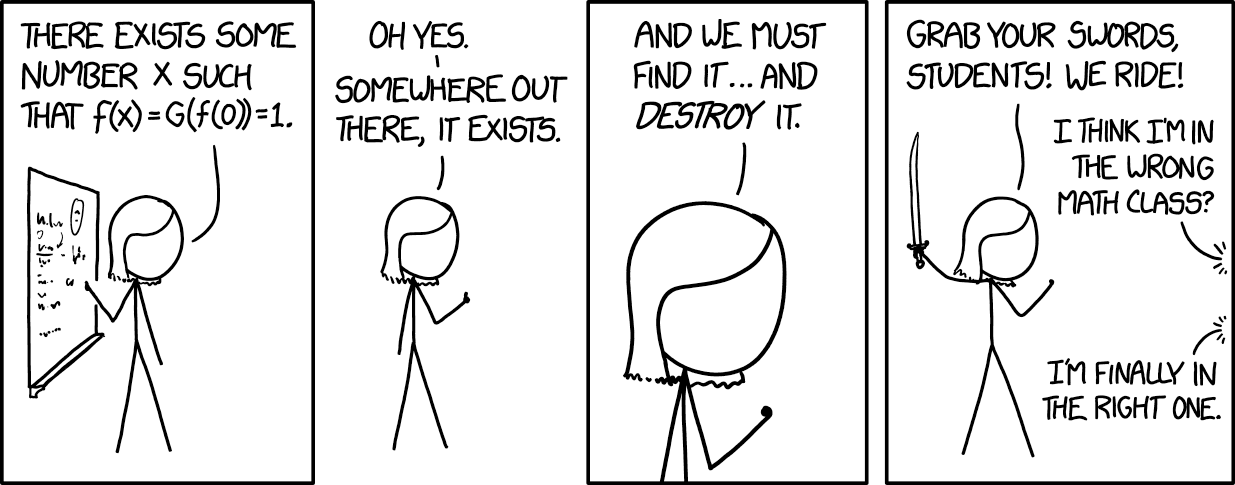
\includegraphics[width=0.9\linewidth]{images/existence_proof_2x} 

}

\caption{Hopefully you are in the right place. Credit   [xkcd.com](https://xkcd.com/1856/)}\label{fig:xkcd-preamble}
\end{figure}

\hypertarget{how-many-kinds-of-people-are-there}{%
\chapter*{How Many Kinds of People Are There?}\label{how-many-kinds-of-people-are-there}}
\addcontentsline{toc}{chapter}{How Many Kinds of People Are There?}

\begin{quote}
There are 10 kinds of people in this world.
Those who understand binary code and those who don't.
--- seen on a T-shirt
\end{quote}

\hypertarget{things-are-about-to-get-meta-right-from-the-start}{%
\section*{Things are about to get meta right from the start}\label{things-are-about-to-get-meta-right-from-the-start}}
\addcontentsline{toc}{section}{Things are about to get meta right from the start}

I'm going to start off this first chapter in a book about data science with an unsubstantiated claim. My claim is this: People love to categorize themselves and others. They love to take quizzes online that tell you ``what kind of person you are'' in some way or another. They love to make statements that begin with, ``there are two kinds of people in this world\ldots{}'' and so on. Ok? That's my claim. It's a bit of a mouthful.

Now, I just made a claim in support of which data \emph{can absolutely} be brought to bear. But I won't use data to support it. What? Why not, for crying out loud?! This is a book about data science!!! The reason is this: this book encourages you to think critically and skeptically about all kinds of ideas, claims, and questions. It tries to show you how to talk about these ideas precisely and not succumb to fallacies and bad intuition. But while trying to develop these skills, it is important to know when we are in turbo critical thinking mode (that's a technical term\footnote{Just kidding; it's not really a technical term.}) and when we're not. Sometimes, we need to be able to say common-sense things and not have to support them.

What \emph{exactly} am I even saying in my claim, you might be thinking? What do you mean by, ``people love to'' do X, where X, like \_\_\_\_\_\_ {[}``blank''{]}, is a stand-in for some of the specific things I mentioned. That everybody does X? Most people? That people who do X derive pleasure above some pleasure threshold, thus designating ``love'' as opposed to ``like?'' You see, I could have tried to make my claim more precise. And I could have found polls and published reports that estimate just how many people have, by choice, taken some kind of person-category-test-thing, or posted funny jokes about ``two kinds of people.'' But I'm just letting my claim stand as a common-sense claim. Just like if I said, people love going to the movies. I wouldn't feel the need to cite a scientific study to support that claim.\footnote{\url{https://digg.com/2019/movie-genre-popularity-1910-to-2018-data}}

Now, if someone is making what to \emph{them} appears to be a common-sense claim but to you appears false or at least non-obvious, you have a few options. You can challenge the assumption and ask for evidence. Or you can accept the assumption, \emph{for argument's sake}, to see where this is going. Hopefully, my claim feels common-sense enough to you too (i.e., we have that in common). If not, I'll just ask you to follow along to see where this is all going\ldots{}

\hypertarget{categories}{%
\chapter{Categories, counts, and kinds}\label{categories}}

\hypertarget{two-kinds-of-people}{%
\subsection*{Two Kinds of People}\label{two-kinds-of-people}}
\addcontentsline{toc}{subsection}{Two Kinds of People}

``There are two kinds of people\ldots{} which one are you?'' questions have become something of an internet meme, particulary with the categorizations represented graphically or pictorially. There is a whole \href{https://2kindsofpeople.tumblr.com/}{blog devoted to them by João Rocha}. The images in Figure \ref{fig:tp-fig} probably need no explanation, as they concern the great \href{https://en.wikipedia.org/wiki/Toilet_paper_orientation}{toilet paper orientation} debate.



\begin{figure}

{\centering 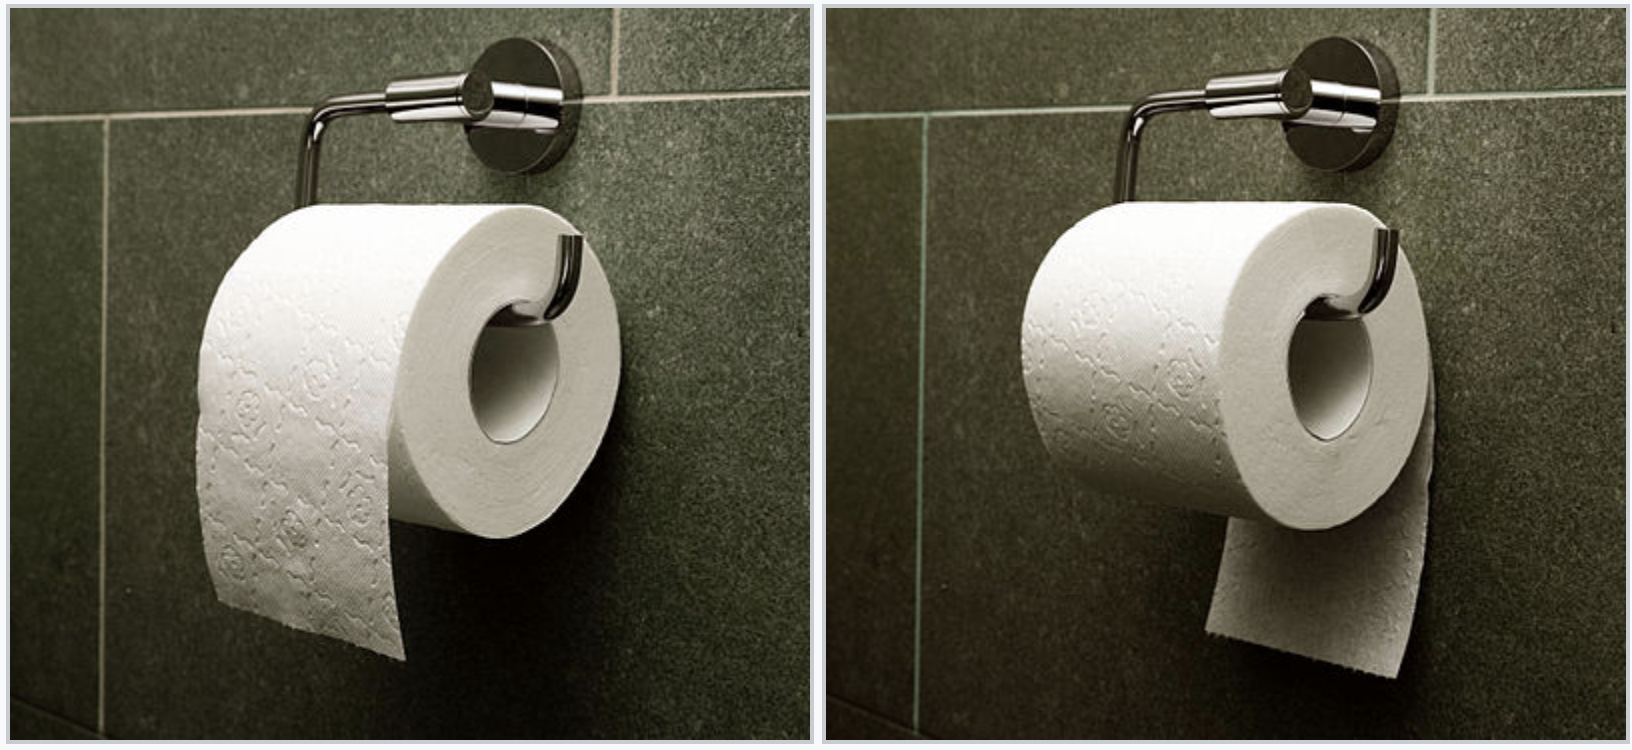
\includegraphics[width=0.9\linewidth]{images/Toilet_paper_orientation_overunder} 

}

\caption{The great debate. Source \href{https://commons.wikimedia.org/wiki/File:Toilet_paper_orientation_over.jpg}{Wikimedia Commons User:Elya}}\label{fig:tp-fig}
\end{figure}

Toilet paper orientation is a distinguishing \textbf{test question} that separates people into one of two ``kinds'' (or ``types'' or ``categories''; sometimes English has several words that are used interchangeably). A fancy word for this ``splitting into two'' is dichotomy (die-COT-uh-mee), from the Greek. A \textbf{dichotomous question} has two possible answers. Here, you choose one way to orient the roll or the other. Let's call this roll choice ``over'' (shown on left) or ``under'' (shown on right). Perhaps you have debated which is better with a friend or family member. In any case, armed with this particular test question, we can go out and collect some data.

\begin{table}[!h]

\caption{\label{tab:tp-table}How people roll}
\centering
\begin{tabular}[t]{lr}
\toprule
 & count\\
\midrule
over & 23\\
under & 17\\
\bottomrule
\end{tabular}
\end{table}

I went ahead and asked 40 people in Washington Square Park in New York City which kind of person they were, and the results are shown in Table \ref{tab:tp-table}. This being a book about data science, you might think I'm going to start calculating proportions right away, for example by saying that 57.5\% of New Yorkers are over-hangers.
Nope. Although you should be able to figure out that proportion conversion, it is not the point I want to focus on right now.

That point I want to focus on is that, based on our data, there \emph{are} indeed two kinds of people here. If, for example, everyone in the world were an under-hanger (heaven forbid), then I couldn't very well say that there were two kinds of people in this world. At least not with regard to toilet paper orientation. It would be like if I presented you with the data in Table \ref{tab:dumb-table}. Looking at that, I can't very well convince you that there are two kinds of people.

\begin{table}[!h]

\caption{\label{tab:dumb-table}Kinds of people in Washington Square}
\centering
\begin{tabular}[t]{lr}
\toprule
  & count\\
\midrule
human & 40\\
not human & 0\\
\bottomrule
\end{tabular}
\end{table}

That all seems pretty obvious, in part because I made up a \emph{tautology} in the second example there. Being a human being is automatically associated with everyone who can be a \emph{kind of person}.

But what if I had gotten exactly the same results for the toilet paper question? What if the data looked like Table \ref{tab:tp-redux}. In this \textbf{alternate universe}, everyone I ask in Washington Square is an under-hanger. Yes, it's one of those scary alternate universes, like the Twilight Zone. Anyway, does that mean that there is only one kind of person when it comes to toilet paper orientation? Well\ldots not necessarily. After all, this was just a \textbf{sample} of people in Washington Square. It was not the whole \textbf{population} of Washington Square, even, let alone New York City, let alone the world.

\begin{table}[!h]

\caption{\label{tab:tp-redux}How people roll (alternate universe)}
\centering
\begin{tabular}[t]{lr}
\toprule
  & count\\
\midrule
under & 40\\
over & 0\\
\bottomrule
\end{tabular}
\end{table}

\hypertarget{samples-and-populations-a-statistical-caveat}{%
\subsection*{Samples and Populations: A Statistical Caveat}\label{samples-and-populations-a-statistical-caveat}}
\addcontentsline{toc}{subsection}{Samples and Populations: A Statistical Caveat}

Samples and populations are sort of a big deal in statistics and data science, where these words have somewhat specialized meanings. Consider the following utterances:

\begin{verbatim}
The population of New York City is 8.6 million
The population of New York City is ethnically diverse
\end{verbatim}

How can both of these statements make sense? In common usage, population often refers to the number or count of people, in a town, area, or country. Among statisticians and data scientists, population refers to a set or collection under consideration. It doesn't have to be a set of people. It could be a set of rats, non-governmental organizations, or domestic flights originating in Chicago. But let's suppose the population does refer to a set of people. The \emph{number} of those people is just one summary about the population, also known as the total \textbf{count}. The proportion of over-hangers is another summary of the population, as is the most-common birth-month. The two statements above would be more consistent if the first were rephrased to be: the population (set of people) of New York City \sout{is} numbers 8.6 million.

If we always had access to all of the members in a population (the set or collection under consideration), the field of statistics wouldn't exist. We would just know a bunch of facts about, say, everyone in the whole world. And that would be that. While it is true that data are becoming more and ubiquitous, don't start betting on the demise of statistics. Even if we did have complete data for everyone in the world today, our population of interest might extend to the world as it will be next month, next year, or ten years from now. That is, we might want to make predictions about the future. In which case, we would want to draw \emph{inferences} and to generalize from the data we have on hand---our sample---to data we don't have---the rest of the (i.e., the future) population. Making inferences from samples to populations will always be a compelling and challenging problem.

Since Washington Square is the center of my universe, that's where I sample. Even if we agreed that our population of interest were confined to Washington Square, we would still find it difficult to collect data on everyone there. There are a lot of them, many of them are on skateboards, and new people keep leaving and entering the park. It turns out, that's okay. We don't actually have to reach everybody to be able to do data science. However, we need to understand that when we sample 40 particular people in Washington Square, we might not get the same exact answers as if we had sampled 40 \emph{different} people. The sampling process introduces an element of \textbf{uncertainty} into our process.

Coming back to our toilet paper debate, if we did find zero over-hangers in one sample, it doesn't guarantee that the number of over-hangers will also be zero in the next. The number may vary from sample to sample. Uncertainty does not, however, mean that the information derived from one sample is useless. In fact, soon we'll see that we can actually learn a lot from a sample simply by recognizing that sample values will vary. We can simulate samples on a computer to see how much they will vary. And then, using our simulations, we will be able to give probabilistic answers to questions like, ``what are the chances that there really are no over-hangers in Washington Square?''

\hypertarget{a-psychological-caveat}{%
\subsection*{A Psychological Caveat}\label{a-psychological-caveat}}
\addcontentsline{toc}{subsection}{A Psychological Caveat}

The section above explored a statistical caveat about drawing conclusions from samples. But another caveat that applies here is more psychological. I have assumed, for this argument, that a person's answer to the toilet paper question is a fairly stable thing and not just a transient state-of-mind. That is, if I asked you tomorrow or next week, your answer would be the same as if I asked you today. For the most part. I'm not saying you can't ever decide to change your mind. But it wouldn't make sense to describe a person as an over-hanger if there were no stability at all to their answer. A transient state-of-mind, by contrast, could be asking someone if they are hungry. Everyone is hungry some of the time, but not all of the time. And it wouldn't make any sense, based on that line of questioning, to imply that there are two kinds of people.

\hypertarget{summarizing-data}{%
\subsection*{Summarizing data}\label{summarizing-data}}
\addcontentsline{toc}{subsection}{Summarizing data}

When I presented my survey results to you in Table \ref{tab:tp-table}, notice that I did not present you with the raw data, but rather with a summary of the data. The particular summary I used was called ``counts'', that is, a total count of how many people responded ``over'' or ``under.'' The raw data, in contrast, would have contained each individual response I collected, labled either with a name of the individual, or perhaps with some other unique identifier (such as a random number), or---if I don't need to keep track of particular individuals---with just a row number. Something like this, if we examine at the first six responses rather than all 40 of them. Raw data:

\begin{table}[!h]
\centering
\begin{tabular}{ccc}
\toprule
row & randomID & response\\
\midrule
1 & 9246 & under\\
2 & 1478 & over\\
3 & 8831 & under\\
4 & 8194 & over\\
5 & 4178 & under\\
\addlinespace
6 & 4243 & under\\
\bottomrule
\end{tabular}
\end{table}

Counts is an example of a \textbf{summary statistic}, which is a fancy term for a number that is derived from the raw data. The count summary is as simple as it gets. It is literally the number of times that each response appears. We might note as well that,

\begin{verbatim}
count(under) + count(over) = total number of responses.
\end{verbatim}

This mathematical statement is true because there are only two possible responses. If there were more than two responses, then I would need to add the counts for each possible response.

Note that the \emph{proportion} of ``over'' responses is also a summary statistic (which is just the counts of ``over'' divided by the total number of responses). Another summary statistic could be the ratio of ``over'' responses (counts) to ``under'' responses. For example, one way people use summary statistics in reporting data is through statements like, ``twice as many people prefer chunky peanut butter to smooth.''

\hypertarget{no-mean-feat}{%
\subsubsection*{No mean feat}\label{no-mean-feat}}
\addcontentsline{toc}{subsubsection}{No mean feat}

\begin{quote}
Whenever someone reports a mean (another word for average) value of some set of data, that is also a summary statistic. Does it make sense to construct an average from responses that are either ``over'' or ``under''? No, it doesn't. That's because \{over, under\} is a categorical response, and you can't average over categories. Unless you're trying to make fun of statistics with a puerile joke. Different versions of this joke appear: ``the average American has one tit and one testicle.'' At the risk of explaining the joke too much, here goes: Tits and testicles can certainly be treated as numerical data, and hence can be averaged. This joke hinges on the fact that the existence of testicles (or tits) is associated with a person's sex, which is categorical and not numerical. Assuming that half of all Americans are female (roughly true), we can't say that the average American is half male and half female. The real ``punch'' of this joke is to suggest that summary statistics about averages are just a bunch of nonsense. What do you think?
\end{quote}

This is about as much as we need to say about summary statistics for the time being. But they'll be back.

\hypertarget{checkpoint}{%
\subsection*{Checkpoint}\label{checkpoint}}
\addcontentsline{toc}{subsection}{Checkpoint}

While focusing on the great toilet paper debate, we've managed to establish some important fundamental ideas.

\begin{itemize}
\item
  Dichotomous questions split people into two kinds, but only as long as it is actually possible for both answers to occur.
\item
  In an alternate universe, people might give different answers than they do in this one. (Seriously, this is an important idea).
\item
  Even when we casually refer to \emph{people}, we may have a particular set of people, a population, in mind. Data about this population are likely to come from a sample, rather than from the whole population, and this fact introduces some uncertainty into claims about the whole population. Data science to the rescue!
\item
  If we have types of people in mind, our questions ought to elicit fairly stable answers
\item
  Clearly, we can ask people questions that prompt them to choose between more than two categories. But ``two types of people'' questions are more fun.\footnote{That was another unsubstantiated claim.} I mean there are so many of them! So\ldots{} does that mean that there really are two types of people? To answer this, we will need to get into another great debate.
\end{itemize}

\hypertarget{dimensions}{%
\chapter{Dimensions}\label{dimensions}}

\begin{quote}
``I always said if I had one breakfast to eat before I die, it would be Wonder Bread toasted, with Skippy Super Chunky melted on it, slices of overripe banana and fresh crisp bacon.''

--- \href{https://nypost.com/2008/07/26/mayors-last-meal-is-a-killer/}{Michael Bloomberg}
\end{quote}

Former NYC mayor Michael Bloomberg is a chunky peanut butter kind of person. Are you? As peanut butter comes in ``smooth'' and ``chunky'' varieties (also known as creamy and crunchy, respectively), this question is also a dichotomous one. However, if we add this test question to our question pool, in addition to the one about toilet paper orientation, we will soon find that having two two-kinds-of-people questions begins to imply more than two kinds of people. Wait, what?

See, back when I went to talk to the people in Washington Square, I also asked them about the great peanut butter debate. As you can see from Table \ref{tab:pb-counts}, smooth came out slightly ahead.

\begin{table}[!h]

\caption{\label{tab:pb-counts}How people spread}
\centering
\begin{tabu} to \linewidth {>{\raggedright}X>{\raggedleft}X}
\toprule
 & counts\\
\midrule
chunky & 17\\
smooth & 23\\
\bottomrule
\end{tabu}
\end{table}

But this second question did not erase the first question about toilet paper. In fact the first few rows of our data from Washington Square are displayed below. Each row, representing one person, now has two columns, labeled ``roll'' (for toilet paper) and ``spread'' (for peanut butter):

\begin{verbatim}
##    roll spread
## 1 under chunky
## 2  over chunky
## 3 under smooth
## 4  over chunky
## 5 under smooth
## 6 under chunky
\end{verbatim}

You may have noticed that among the first six people for whom I have shown data, none of them answered both over and smooth. But such response pairs exist. In fact, if we count each combination as it occurs--that is, under-chunky, over-chunky, under-smooth, and over-smooth--we get the results shown in Table \ref{tab:tpxpb}. There are four combinations, because we have two questions with two possibilities (dichotomies) for each.

Before you read on, it's a good time to ask yourself if you can answer the following questions (answers in the footnote): (a) if there were two questions with three categories each, how many combinations could be observed? (b) if there were three dichotmous questions, how many combinations could be observed?\footnote{(a) If the categories for each question are A, B, and C, we can get AA, AB, AC, BA, BB, \ldots{} etc. We multiply the number of categories as many times as we have questions. So 3*3 = 9. (b) This time we have three questions, and for each one we have two options, so there are 2*2*2=8 possible combinations.}

\begin{table}[!h]

\caption{\label{tab:tpxpb}Two questions}
\centering
\begin{tabular}[t]{lrr}
\toprule
  & chunky & smooth\\
\midrule
over & 10 & 13\\
under & 7 & 10\\
\bottomrule
\end{tabular}
\end{table}

Table \ref{tab:tpxpb} is an example of a kind of table that is so common in data science, it has its own name. Three of them, in fact. It is sometimes called a cross table (or crosstab), or a \textbf{two-way table} (makes sense), but most commonly it is known as a \textbf{contingency table} (wha? I'll explain later) I'm sorry that there are three names for the same thing. Really I am.

\begin{quote}
If you're like me, you can't resist paying some attention to the values in the Table \ref{tab:tpxpb}. For example, you might notice that one of the cells of the table (over AND smooth) has the highest number of people in it. We can say that this is the \textbf{modal} category, referring to the \textbf{mode}, which is the most common value in a distribution of values. We have four possible values in this example.
\end{quote}

Ok, now things are about to get deep. This first module is ``How Many Kinds of People are There?'' And we've now explored how using two two-kinds questions leads to four types. You've probably figured out yourself that you have to multiply the number of categories in each of the questions, and that tells you how many ``buckets'' you can have overall. But still, there are different ways to arrive at a certain number of buckets.

\begin{table}[!h]

\caption{\label{tab:newpb}PB preference}
\centering
\begin{tabular}[t]{lr}
\toprule
 & counts\\
\midrule
chunky & 13\\
don't care & 3\\
hate all & 4\\
smooth & 20\\
\bottomrule
\end{tabular}
\end{table}

Consider Table \ref{tab:newpb} in contrast to \ref{tab:tpxpb}. We've now given people four choices to express their peanut butter preference. In addition to chunky and smooth, they can also choose to say that they hate all peanut butter or don't care. We now have four kinds of people. But since we make the determination of what kind of person you are using just one question, we say that there is one \textbf{dimension} (in this case, peanut butter preference) along which people can be divided into four groups. In Table \ref{tab:tpxpb}, there were two dimensions, a dimension of peanut butter and a dimension of toilet paper. Notice that this word, dimension, is used in much the same way as when we refer to geometric space as being two-dimensional (e.g., a drawing on flat sheet) or three-dimensional (e.g., a solid object, or sometimes a drawing that creates the illusion of looking at a solid object.) The three dimensions of space are often labeled something like (x, y, z). Here, our two dimensions could be labeled (pb, tp). The order doesn't matter. We are merely indicating that there are two different variables used in categorizing our data (people, in this case). To summarize, in Table \ref{tab:tpxpb}, we have two dimensions and four kinds. In Table \ref{tab:newpb}, we have \emph{one} dimension and four kinds.

So far so good: two questions, two dimensions, right? Well\ldots{} maybe. We already saw that if a question does not actually divide people into kinds, because only one answer appears, then it doesn't really count. It is not a dimension, because it is not really a variable. It does not vary; it is constant. In our contingency table representation, this might look like the left side of Table \ref{tab:tpxpb-alt}. In an alternate universe, no one prefers smooth to chunky. Another way to say it is that the peanut butter question is not \textbf{informative} because it has no \textbf{variance}. Everyone in our sample is the same.

\begin{table}[!h]
\caption{\label{tab:tpxpb-alt}Two questions (alternate universes)}

\centering
\begin{tabular}[t]{lrr}
\toprule
  & chunky & smooth\\
\midrule
over & 23 & 0\\
under & 17 & 0\\
\bottomrule
\end{tabular}
\centering
\begin{tabular}[t]{lrr}
\toprule
  & chunky & smooth\\
\midrule
over & 0 & 23\\
under & 17 & 0\\
\bottomrule
\end{tabular}
\end{table}

But now consider the alternate universe on the right of Table \ref{tab:tpxpb-alt}. In that case, everyone who is an over-hanger of toilet paper prefers smooth peanut butter, and everyone who is an under-hanger prefers chunky. If this is the case, there are only two kinds of people, at least in our sample. Those who over-hang \emph{and} prefer smooth and those who under-hang \emph{and} prefer chunky. But does it make sense to say there are two dimensions? We did ask two different questions!

You might reason about it the following way: in our sample, if I ask anyone just one of the two questions--about either toilet paper or peanut butter--then I immediately know the answer they would give to the other one. Another way to say this is that the answer to one question completely \emph{determines} the answer to the other, and thus the relationship between these questions (really, the answers) is \textbf{deterministic}. I don't actually have to ask two questions, other than to establish in the first place that I didn't have to. And since I only get information from one question, there is only one dimension.

\hypertarget{independence-association-and-contingency}{%
\section*{Independence, Association, and Contingency}\label{independence-association-and-contingency}}
\addcontentsline{toc}{section}{Independence, Association, and Contingency}

\begin{quote}
This section title sounds like a philosophy book by the late Richard Rorty.
--- inner voice
\end{quote}

We just spent a little bit of time in an alternate universe, a bizarro world in which knowing how someone prefers to orient their toilet paper tells you what style of peanut butter they like, and \emph{vice versa}. Notice that this knowing-about relationship is symmetric, and that in fact, the two representations as shown in Table \ref{tab:tpxpb-alt2way} are informationally equivalent.

\begin{table}[!h]
\caption{\label{tab:tpxpb-alt2way}Alternate universe (two equivalent ways)}

\centering
\begin{tabular}[t]{lrr}
\toprule
  & chunky & smooth\\
\midrule
over & 0 & 23\\
under & 17 & 0\\
\bottomrule
\end{tabular}
\centering
\begin{tabular}[t]{lrr}
\toprule
  & over & under\\
\midrule
chunky & 0 & 17\\
smooth & 23 & 0\\
\bottomrule
\end{tabular}
\end{table}

In our regular universe, however, this relationship was not observed. In Table \ref{tab:tpxpb}, all four possible combinations occur. When knowledge about a person's answer to one question provides information about their answer to another question, we say that the two answers are \textbf{contingent} upon one another. This is the reason we called the two-way table a contingency table in the first place, although it is still called that even when two answers are not contingent. Go figure. Contingent is another word for \textbf{dependent}. To make matters worse, we \emph{also} often say that the two responses are \textbf{associated}.

In our bizarro world scenario, one answer completely determines the other. This \textbf{deterministic} relationship is one extreme in the spectrum of association/dependence/contingency. It expresses a certainty in knowing the answer to one question if we know the answer to another. At the other extreme, if the two responses are not at all associated/dependent/contingent, then we say that they are \textbf{independent}. To say that two responses are independent is to assert that knowing one of them does not give you any information about what the other one might be. This would have been my intuition, at least, about toilet paper and peanut butter. Somewhere in the middle, we might say that one answer gives you some information, but not certainty about another answer. Whether two answers are independent or mildly associated with one another is an empirical question, which means we should try to answer it with data. In bizarro world, where they were deterministically related, we might reasonably want to know why. Could there be a gene that controls both toilet paper orientation and peanut butter preference at the same time?

\hypertarget{latent-factors-and-measurement}{%
\section*{Latent Factors and Measurement}\label{latent-factors-and-measurement}}
\addcontentsline{toc}{section}{Latent Factors and Measurement}

\begin{figure}

{\centering 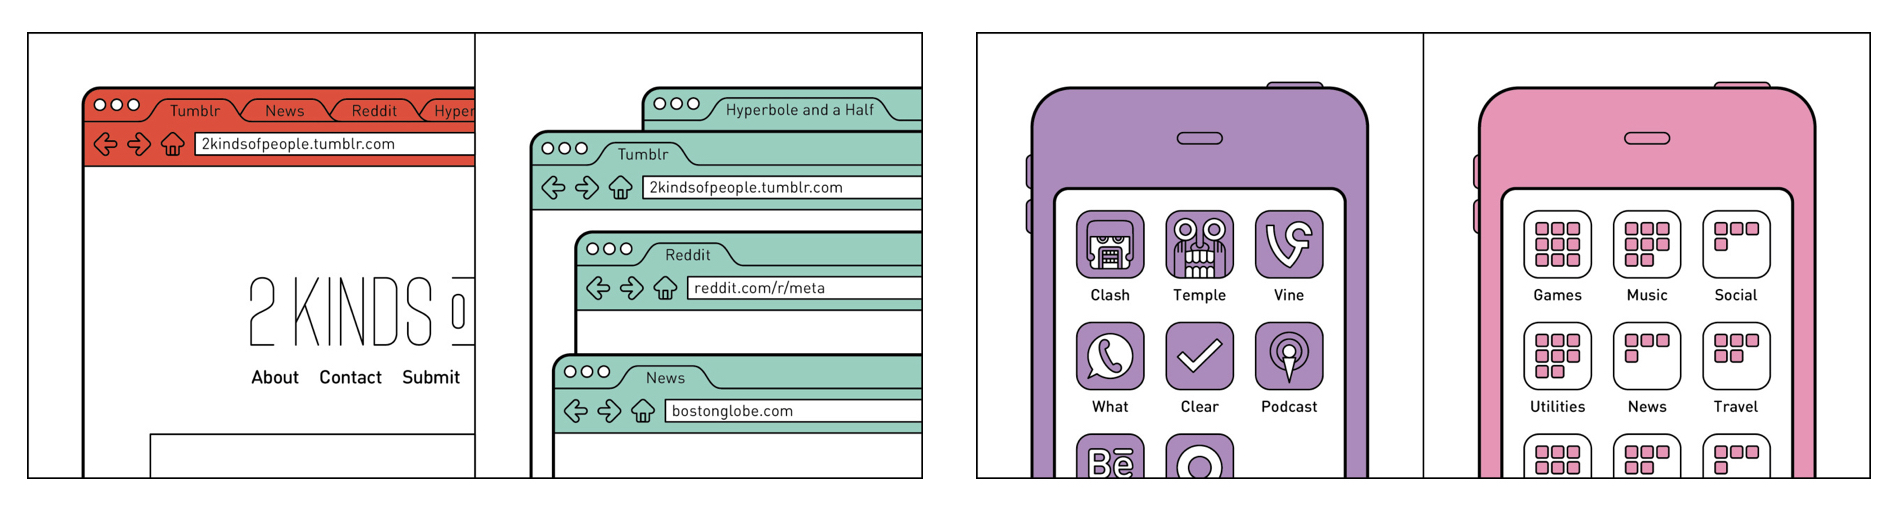
\includegraphics[width=0.9\linewidth]{images/two-two-kinds} 

}

\caption{Two more two-kinds questions}\label{fig:apps-windows}
\end{figure}

Figure \ref{fig:apps-windows} (\href{https://2kindsofpeople.tumblr.com/}{source}) shows two more two-kinds of people graphics from João Rocha's blog. I bet that you can identify yourself with one of the two images in each pair. I certainly can. But ask yourself, given our discussion above, do you think the choices a person would identify in each case above are independent or not independent (e.g., contingent, associated, dependent)?

In contrast to the toilet paper and peanut butter questions, which at least appear to be about totally different things, these two dichotomies have something similar going on in each of them. The choice on the left is about organizing your desktop browser, either in tabs or as separate windows. The choice on the right is about organizing apps in your smartphone, either loose or in folders. We might say that both of them get at a tendency to organize your digital environment. Call it digitidness (short for digital tidiness). This tendency, we may imagine, might even carry over into non-digital environments, like your actual desk, bookshelf, or filing cabinet.

What we've done here is to try to explain the association between responses to the two questions (assuming that there is, i.e.~that they are not independent) by appeal to some underlying \textbf{latent factor}. We say a factor is latent (meaning hidden) because we don't observe digitidiness itself directly, but we only observe tidy browsers or smartphone app folders. Perhaps you can think of another candidate factor besides digitidiness. In any case, we might propose that both of the two two-kinds questions in Figure \ref{fig:apps-windows} are in effect indirect \textbf{measurements} of the same factor. If so, this could explain why the two answers would be associated.

\begin{quote}
Notice that a \textbf{factor} is also a dimension, in the sense we used before. We could have said ``latent dimension'', but we tend to use the word factor when we are drawing attention to the specific nature of the dimension rather than just counting. We also sometimes use the word \textbf{trait}. At least in psychology, trait tends to be reserved for stable psychological factors. Thus ``stress'' can be a factor but not a trait, whereas ``social anxiety'' may be a trait, if it is persistent. In this case, digitidiness might be considered a trait (and thus also a factor and a dimension).
\end{quote}

Contrast this with toilet roll orientation, which we can observe directly just by looking in someone's bathroom. (We assume that they are telling the truth when they answered our questions, but we could in principle verify it.) It was only in the bizarro world when toilet roll orientation and peanut butter preference were perfectly related that we started to wonder if there maybe \emph{was} an underlying genetic factor. Genetic factors were once not directly observable either, but we assumed them for explanatory value. Today we can of course observe specific genetic variation, although there are still many gaps in our understanding of the relationship between genes and observed behaviors.

Consider some data again, in two possible worlds, shown in Table \ref{tab:tabsxapps}. On the left, we have the deterministic scenario we saw before. As before, we identified this situation as having two kinds of people and really just one dimension. In contrast to before, where we had no real explanation for this coincidence, we attribute it now to some factor, like digital tidiness.

\begin{table}[!h]
\caption{\label{tab:tabsxapps}Possible data for digital tidiness}

\centering
\begin{tabular}[t]{lrr}
\toprule
  & app-folders & apps-loose\\
\midrule
browser-tabs & 21 & 0\\
browser-windows & 0 & 19\\
\bottomrule
\end{tabular}
\centering
\begin{tabular}[t]{lrr}
\toprule
  & app-folders & apps-loose\\
\midrule
browser-tabs & 16 & 6\\
browser-windows & 5 & 13\\
\bottomrule
\end{tabular}
\end{table}

But now consider the possible results in the table on the right. Since all four possible quadrants have non-zero counts, we see that knowing whether someone organizes their browser using tabs does not completely (i.e., \emph{deterministically}) specify whether or not they put their apps into folders. On the other hand, one answer \emph{does seem to be associated} with the other. Notice that the values are still much higher in the diagonal ``buckets'' that we think of as indicating the presence or absence of digitial tidiness. These are the tabs-folders bucket (tidy) or the windows-loose bucket (not tidy). We say that the tidiness factor appears to explain much of the observed range, or \textbf{variance}, in responses to the two questions. But it doesn't explain all of it, since there are people (11 out of 40, in this case) who don't fall into one of these buckets.

This situation on the right is probably more realistic. After all, very few things in this world are absolute (unlike in bizarro world). So now the big question re-emerges: are there two kinds of people or four? One dimension, or two? It's sort of\ldots like\ldots in between\ldots?

\textbf{Golda says}: Although digitidiness explains a lot of what we see in our data, it doesn't explain it all. I believe that desktop tidiness and mobile tidiness are different, if related, tendencies. For example, when we use mobile phones, we're typically on-the-go and have less time. If we knew more about the people in our sample, we might see that these discrepancies in the organization of apps and tabs actually relate to other aspects of their lives. So, I say there are two dimensions.

\textbf{Sidney says}: Digitidiness is the only real factor here, but people may not always be consistent in these particular behaviors. Also some people are only sort-of-tidy, and apply this tidiness unevenly and randomly. These two-kinds of people choices don't leave room for shades of gray, so that's what we're seeing in the mixed categories where people are tidy in one environment and not in another. But ultimately there is really just one dimension here.

\textbf{What do you think?}

\hypertarget{test-indep}{%
\chapter{Tests of independence: A first look starring alternate universes}\label{test-indep}}

So far, we have looked at some data in two-way tables and judged them by inspection. That is, we looked at them and said, these two responses \emph{appear} to be deterministically related, or they appear to be associated but not deterministically, or they appear to be independent. But we acknowledged that our data come from a sample, and that on another day (on in another universe with rules the same as this one), we might have observed slightly different data.

It is worth noting that a single dataset often can't tell us for sure whether two variables are independent or associated (aka dependent/contingent), and whether or not an association is a deterministic one. (Two variables cannot be deterministically independent; that would be a self-contradiction.)

In this chapter, we'll take a first look at how a particular two-way table \emph{might} have come about, and thus how it might have come out differently. Let's suppose that we observe the data summarized here:

\begin{table}[!h]

\caption{\label{tab:indep-sim}Another alternate universe}
\centering
\begin{tabular}[t]{lrr}
\toprule
  & chunky & smooth\\
\midrule
over & 17 & 6\\
under & 5 & 12\\
\bottomrule
\end{tabular}
\end{table}

It looks like certain pairs of outcomes are coming up more than we would expect ``by chance'' if the answers were not associated. Equivalently, it looks like there is an association between these variables, but let's investigate further. Let's take the cell with the largest number of people in it, or the modal value. In this case, the mode occurs for people who answer over and chunky. Which was 17 out of 40.

Now consider what contributes to making this particular value what it is. For example, what would make it bigger? Well, if there were more over-hangers than under-hangers, that would tend to increase the number of people who could be \emph{both} over-hangers and chunky-spreaders. Similarly, if there were more chunky-spreaders. Also, if there were just more people in our sample, then of course we could have more people in this cell of the table. And all of the above arguments could work in reverse, if we lowered any of those particular numbers.

What if, for argument's sake, we fixed the total number of people, the number over-hangers among them, and the number of chunky-spreaders among them. We're going to keep these values constant while letting the individual table elements vary. The technical term for this, by the way, is fixing the \textbf{marginal} values. This is because the sums of the columns (22 and 18) and the sums of the rows (23 and 17), when written at the bottom and side of the table, are called margins (just like the margins of a page). We could still have fixed the marginal values and have different values in the table. For example,

\begin{table}[!h]
\caption{\label{tab:unnamed-chunk-8}Yet more alternate universes!}

\centering
\begin{tabular}[t]{lrr}
\toprule
  & chunky & smooth\\
\midrule
over & 19 & 4\\
under & 3 & 14\\
\bottomrule
\end{tabular}
\centering
\begin{tabular}[t]{lrr}
\toprule
  & chunky & smooth\\
\midrule
over & 13 & 10\\
under & 9 & 8\\
\bottomrule
\end{tabular}
\end{table}

Notice that the row and column sums are the same. But on the left we would say an association between the variables appears even more clear, whereas on the right, it appears less obvious. Can you see why?

Recall that the actual data summarized in a two-way table originally came from some observation sample. There were 40 people sampled, and they were each asked two questions. Before we tabulated them, the data might have looked something like this:

\begin{table}[!h]
\centering
\begin{tabular}{l|l}
\hline
Peanutbutter & Toiletpaper\\
\hline
Smooth & Under\\
\hline
Chunky & Over\\
\hline
Chunky & Under\\
\hline
Chunky & Over\\
\hline
Smooth & Under\\
\hline
\end{tabular}
\end{table}

Now suppose we wrote every person's response to the peanut butter question on an index card, shuffled them randomly, and then re-distributed them. We then did the same for the toilet paper question. We did this one question at a time, separately. Finally, we ask our sample to show us their cards, and we treat these paired observations as a new data set. We generate a new two-way table from the results. If we do all this, then we will have kept the total number of people the same, as well as the total number of ``over'' answers and ``chunky'' answers. Moreover, since we shuffled responses to each question separately, there is absolutely no way for someone's randomly assigned answer to one question (the index card they got for peanut butter) to influence their randomly assigned answer to the other (the index card for toilet paper). The answers should, by definition, be independent.

\hypertarget{rise-of-the-machines}{%
\section*{Rise of the machines}\label{rise-of-the-machines}}
\addcontentsline{toc}{section}{Rise of the machines}

Well, we can do this shuffling experiment very easily on a computer. And we can very easily repeat it 1000 times. So, the question we might then ask is, how many times out of 1000 such \textbf{simulations} do we get a value for over and chunky that is as large as (or bigger even) than 17?

The code to do this, and to visualize the outcome, is below. (You do not need to understand this code yet, but some of it might make sense to you).

\begin{Shaded}
\begin{Highlighting}[]
\NormalTok{simulated\_overchunky }\OtherTok{=} \FunctionTok{c}\NormalTok{() }\CommentTok{\#initialize empty vector}
\ControlFlowTok{for}\NormalTok{(i }\ControlFlowTok{in} \DecValTok{1}\SpecialCharTok{:}\DecValTok{1000}\NormalTok{)\{}
  \CommentTok{\# the sample() function does the shuffling}
\NormalTok{  shuffle\_data}\SpecialCharTok{$}\NormalTok{Peanutbutter }\OtherTok{=} \FunctionTok{sample}\NormalTok{(shuffle\_data}\SpecialCharTok{$}\NormalTok{Peanutbutter) }
\NormalTok{  shuffle\_data}\SpecialCharTok{$}\NormalTok{Toiletpaper }\OtherTok{=} \FunctionTok{sample}\NormalTok{(shuffle\_data}\SpecialCharTok{$}\NormalTok{Toiletpaper)}
  \CommentTok{\# the table() function does the tabulating}
\NormalTok{  simulated\_overchunky[i] }\OtherTok{=} \FunctionTok{table}\NormalTok{(shuffle\_data)[}\StringTok{"Chunky"}\NormalTok{,}\StringTok{"Over"}\NormalTok{]}
\NormalTok{\}}

\CommentTok{\# plot the results using a histogram}
\FunctionTok{hist}\NormalTok{(simulated\_overchunky, }
     \AttributeTok{main =} \StringTok{""}\NormalTok{,}
     \AttributeTok{xlab =} \StringTok{"Count"}\NormalTok{, }
     \AttributeTok{breaks =} \FunctionTok{seq}\NormalTok{(}\DecValTok{0}\NormalTok{,}\DecValTok{20}\NormalTok{,}\DecValTok{1}\NormalTok{))}
\FunctionTok{abline}\NormalTok{(}\AttributeTok{v=}\DecValTok{17}\NormalTok{, }\AttributeTok{lwd=}\DecValTok{2}\NormalTok{, }\AttributeTok{col=}\DecValTok{3}\NormalTok{, }\AttributeTok{lty=}\DecValTok{2}\NormalTok{)}
\end{Highlighting}
\end{Shaded}

\begin{figure}

{\centering 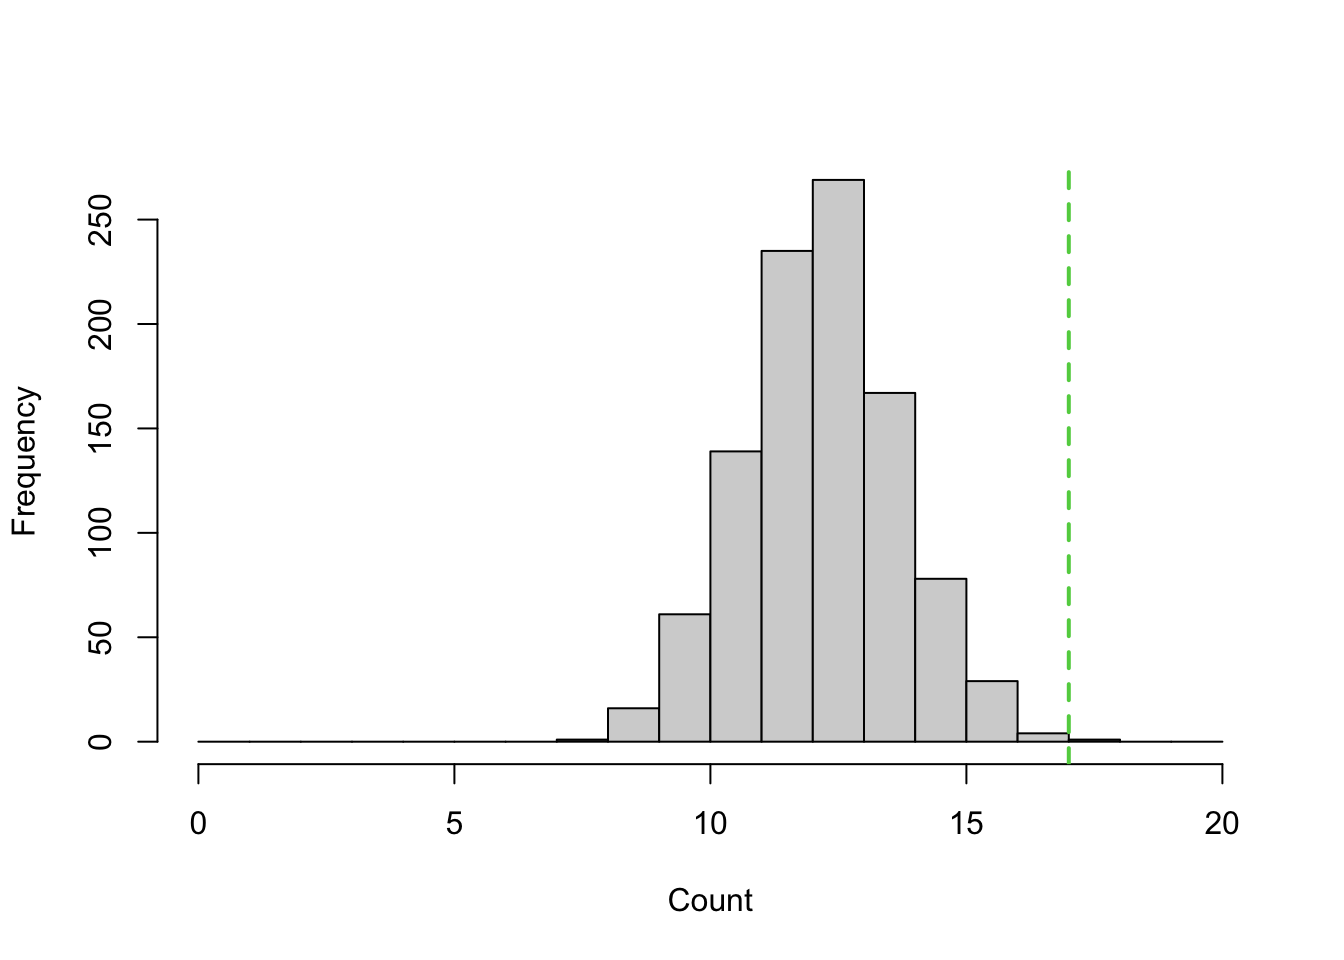
\includegraphics[width=0.9\linewidth]{carpedatum_files/figure-latex/shuffle-test-1} 

}

\caption{Counts of ``over and chunky'' after 1000 shuffling simulations}\label{fig:shuffle-test}
\end{figure}

Figure \ref{fig:shuffle-test} is histogram, or a bar plot of count data. We will cover histograms in detail the next chapter, so don't worry too much if some of this is still confusing. The main thing to notice is that green dotted line at 17, and this: in our 1000 shuffling experiments, we got values greater than or equal to 17 only 5 times. (You probably can't \emph{see} this in the histogram, but if you run the code, you can ask R to report this: \texttt{length(which(simulated\_overchunky\ \textgreater{}=\ 17))}) The rest of the time, the values were smaller, and typical values were around 13.

This simulation we just carried out is a way of validating our intuition, from inspection of Table \ref{tab:indep-sim}, that 17 was a high value \emph{if toilet paper orientation and peanut butter preference} were indeed independent. What we showed is that, if indeed the two variables were independent, that such values would be observed only rarely. Since this value was observed on our first day out in the park (in this scenario), we begin to doubt independence. If on the other hand, we had observed 13 over-chunky people (out of 40, and with the same marginal values as before), then we would say that this observation seems quite consistent with independence. Because values near 13 occur very often in our shuffling simulation.

\hypertarget{hypothesis-testing-just-happened}{%
\section*{Hypothesis testing just happened}\label{hypothesis-testing-just-happened}}
\addcontentsline{toc}{section}{Hypothesis testing just happened}

What we just did is in fact an example of a \textbf{hypothesis test}. In the statistical framework of hypothesis testing, we have a \textbf{null hypothesis} (usually, a skeptical position) and an \textbf{alternative hypothesis}. Here our null hypothesis was that the two variables represented in our response data are independent. Our alternative hypothesis was that people who are over-hangers are truly more likely to be chunky-spreaders. We didn't state this hypothesis at the outset. But it was implied by the fact that we were investigating this ``high'' value in the contingency table. If you take a regular statistics class, however, you will see that, when it comes to \emph{inference}, it is quite important to take care in constructing your null and alternative hypotheses. For now, we just want to get the main idea.

The main idea was that we simulated what data might look like under the null hypothesis (independence) and checked if our observations were consistent with that or not. Consistent (with the null) results would mean that we cannot ``reject'' the null hypothesis, while highly inconsisent results give us justification to ``reject the null'' in favor of the alternative. In this example, we would probably reject the independence assumption (null) in favor of the alternative. The independence assumption was consistent with values around 13 plus or minus 3 (i.e., the range of 10-16). But 17 is unusually high.

\hypertarget{caveats}{%
\section*{Caveats}\label{caveats}}
\addcontentsline{toc}{section}{Caveats}

\textbf{Rare events still do happen, rarely.} What our simulation showed us is that high values do still happen by chance. Even if the variables were independent, if we sent 1000 people out in the world to collect data from samples of 40 people each, \emph{some} of those people would observe large values that \emph{look} associated. This is to be expected. This is why it is important, if we are seeking the truth, that we not game the system by checking over and over again until we get an answer that we like. This would be like rolling double-sixes on the fourteenth try and then saying ``ha! see, I told you I was lucky.''

\textbf{What about the other cells in the table?} You might be wondering how we can do this whole simulation just for the one cell in the table that corresponded to over-chunky. You're right to wonder this (if you are). In time, we will see that we can do independence-tests (or other hypothesis tests) more democratically by examining all of the cells in the table and how they differ from what we would expect under the independence (null) hypothesis. For now, though, note the following. Each of our variables is dichotomous, and we fixed the row and column marginals (totals). So if over-chunky is high, and total count of chunky is held fixed, that means that under-chunky must be low. Our test would have gone the same way if we sought to explain that cell. So, too, must over-smooth be low (lower than it would be under independence assumptions).

\hypertarget{sampling-simulations-and-randomness}{%
\section*{Sampling, simulations, and randomness}\label{sampling-simulations-and-randomness}}
\addcontentsline{toc}{section}{Sampling, simulations, and randomness}

In the last section, we used the \texttt{sample()} function in R to shuffle some values in our simulation. That is, starting with a data set of 40 responses (for example, 23 ``over'' responses and 17 ``under'' responses), we wanted to reassign these responses randomly among the people in our observation sample. What if we wanted to simulate the original set of answers in the first place? It turns out we can also use the computer without collecting any data at all.

To reproduce the exact example above, it would suffice to write down a series of values like this (over, over, over, over, \ldots, over, under, under, \ldots{} , under), 23 overs and 17 unders, and then shuffle them. Boom. The first shuffle is our simulated data. But that procedure wouldn't work if we wanted a sample of 3, would it? If we want to be able to simulate data with different sample sizes, we need another approach.

\hypertarget{tossing-virtual-coins}{%
\subsection*{Tossing (virtual) coins}\label{tossing-virtual-coins}}
\addcontentsline{toc}{subsection}{Tossing (virtual) coins}

Let's simplify things for a minute and assume that in actuality, people are equally likely to be over-hangers or under-hangers. Or that for whatever dichotomous question we want to ask, the likelihood of either responses is 50\%.
If you want to simulate an event that has a 50\% chance (or probability of 0.5), you can toss a coin. If we want to randomly assign 10 people to one of two groups, say the Sharks and the Jets, we can do the following. First, decide that Heads we choose Sharks (this is, of course, arbitrary). Then, for each person, flip a coin. If heads, then assign them to Sharks. If tails, assign them to Jets.

Another way to do this is to put two poker chips into a hat, say a red chip (for Sharks) and a blue chip (for Jets). Then blindly reach into the hat and pick out one chip, record the value, and then put it back and shake the hat before the next draw.

Pulling a chip out of a hat or tossing a coin are equivalent manifestations of the \emph{ideal} process of sampling a random event with a 50\% chance. This is actually a profound idea. The coin toss or hat draw are concrete, mechanical processes. Each has two possible outcomes (heads/tails or red/blue), and, for all intents and purposes, the outcomes in both cases are equally likely. We human beings have learned to abstract from both of these mechanical processes to an idea of a \textbf{stochastic process} which is the same thing as a random process and the exact opposite of a deterministic process. This abstract process requires that we have a \textbf{state space}, which is just a \textbf{set of possible outcomes} (mathematicians refer to some sets as spaces). As long as the set has two possibilities, it doesn't really matter whether we label them heads/tails, over/under, red/blue, Sharks/Jets, or 0/1, because the label can always be assigned to mean whatever we want it to mean (just as we decided heads corresponds to Sharks). In addition to the state space, we abstract the idea of the \textbf{sampling process}. This is what ``picks'' out one of the possible outcomes. Like the coin-flip or the hat-draw. And it is this sampling process where the probability of the outcome appears.

We can in fact simulate this sampling process on the computer in R. In fact we can do it several different ways. Here, first, is a more or less direct translation of what our mechanical process would do. The key enabling function here is called \texttt{sample()}, which works just like pulling chips out of a hat. We will tell \texttt{sample()} what's in the hat by defining a set (a vector, in R) called \texttt{coinstates}. Then we will sample once from the hat for each person.

\begin{Shaded}
\begin{Highlighting}[]
\FunctionTok{set.seed}\NormalTok{(}\DecValTok{8675309}\NormalTok{) }\CommentTok{\# I\textquotesingle{}ll explain this later }

\NormalTok{coinstates }\OtherTok{\textless{}{-}} \FunctionTok{c}\NormalTok{(}\StringTok{"H"}\NormalTok{,}\StringTok{"T"}\NormalTok{)}
\NormalTok{numPeople }\OtherTok{\textless{}{-}} \DecValTok{10}

\CommentTok{\# start a blank list to hold my team assignments}
\NormalTok{teamassignments }\OtherTok{\textless{}{-}} \FunctionTok{c}\NormalTok{()}

\CommentTok{\# now, go one by one; this is called a programming "loop"}
\ControlFlowTok{for}\NormalTok{ (i }\ControlFlowTok{in} \DecValTok{1}\SpecialCharTok{:}\NormalTok{numPeople) \{}
  \DocumentationTok{\#\# toss coin and observe}
\NormalTok{  coinresult }\OtherTok{\textless{}{-}} \FunctionTok{sample}\NormalTok{(coinstates, }\DecValTok{1}\NormalTok{) }\CommentTok{\# the 1 means sample once}
  \CommentTok{\# associate outcome with team assignemnt}
  \ControlFlowTok{if}\NormalTok{ (coinresult }\SpecialCharTok{==} \StringTok{"H"}\NormalTok{) \{}
\NormalTok{    team }\OtherTok{\textless{}{-}} \StringTok{"Sharks"}
\NormalTok{  \} }\ControlFlowTok{else} \ControlFlowTok{if}\NormalTok{ (coinresult }\SpecialCharTok{==} \StringTok{"T"}\NormalTok{) \{}
\NormalTok{    team }\OtherTok{\textless{}{-}} \StringTok{"Jets"}
\NormalTok{  \}}
  \CommentTok{\# record team assignment}
\NormalTok{  teamassignments }\OtherTok{\textless{}{-}} \FunctionTok{c}\NormalTok{(teamassignments, team)}
\NormalTok{\}}

\NormalTok{teamassignments}
\end{Highlighting}
\end{Shaded}

\begin{verbatim}
##  [1] "Jets"   "Sharks" "Jets"   "Sharks" "Jets"   "Sharks" "Sharks" "Sharks"
##  [9] "Jets"   "Sharks"
\end{verbatim}

Voila. The \texttt{sample} function did the apparent work of the coin flip or, equivalently, picking a ``Heads'' or ``Tails'' out of a hat containing both. Just as good, right? Notice that (a) we only got four Jets, not five, and (b) sometimes we got three Sharks in a row. That's randomness for you.

\begin{quote}
Technically, it is pseudo-randomness. Notice the first line of the code where I set the ``seed'' for the random number generator. What this does is make sure that every time I run this code I get the same results. If that seems not random to you, I don't blame you. But here are some important things to keep in mind. First, even though using this random seed makes my experiment repeatable, I still have no idea what the results are going to be until I run it the first time. Second, if I change the seed, even by a tiny amount, then I will once again have no idea. Try it yourself. Note that if you do not declare a random seed, then the computer will effectively choose one for you, perhaps by using the exact computer time in milliseconds. This way the results will still be different every time you run it. If you want to read (a little bit) more about randomness, see the Appendix.
\end{quote}

If you're thinking we could have removed the coin from this process, you're right. Coins are not essential to this process. We could imagine a mechanical device that drops marbles into jars directly, provided that we believed the marble dropping process was equivalent to the coin flip in terms of 50/50 chances. In R, here is a faster way. We just sample out of a ``hat'' containing each of the team names.

\begin{Shaded}
\begin{Highlighting}[]
\FunctionTok{set.seed}\NormalTok{(}\DecValTok{8675309}\NormalTok{) }\CommentTok{\# same seed, on purpose}

\NormalTok{teamnames }\OtherTok{\textless{}{-}} \FunctionTok{c}\NormalTok{(}\StringTok{"Sharks"}\NormalTok{,}\StringTok{"Jets"}\NormalTok{)}
\NormalTok{numPeople }\OtherTok{\textless{}{-}} \DecValTok{10}

\NormalTok{teamassignments }\OtherTok{\textless{}{-}} \FunctionTok{sample}\NormalTok{(teamnames, numPeople, }\AttributeTok{replace=}\ConstantTok{TRUE}\NormalTok{)}
\NormalTok{teamassignments}
\end{Highlighting}
\end{Shaded}

\begin{verbatim}
##  [1] "Jets"   "Sharks" "Jets"   "Sharks" "Jets"   "Sharks" "Sharks" "Sharks"
##  [9] "Jets"   "Sharks"
\end{verbatim}

Well, that was simpler. Notice also that by using the same random seed, I got the same team assignments, even though the code was completely different. (By the way, the {[}1{]} and {[}9{]} here are just index--count--values that R writes out when the data flow across multiple rows. So you know that the first value on the second row is in fact the 9th element of the vector.)

There's another difference here, which is that instead of going one by one for each person, I made the selection all at once by passing the number of people to the sample function instead of asking for one sample. Because I'm sampling \texttt{numPeople} times and there are only two outcomes (``in the hat''), I have to add the argument \texttt{replace\ =\ TRUE} when I call the \texttt{sample()} function. This means that after I look at the result, I put it back in the hat (I replace it), and then draw again. Otherwise, I could sample only as many times as I have choices.

Sampling \emph{without replacement} is suitable if, as in the independence test from earlier, all I wanted was to put a set of choices in random order. As we said, this is like shuffling a deck of cards by dropping the deck into a big bag, shaking it, and then pulling the cards out one by one. No replacement.

\hypertarget{but-some-observations-do-occur-more-than-others}{%
\subsection*{\texorpdfstring{But some observations \emph{do} occur more than others}{But some observations do occur more than others}}\label{but-some-observations-do-occur-more-than-others}}
\addcontentsline{toc}{subsection}{But some observations \emph{do} occur more than others}

To complete the functionality of our data-generating machine, we need a way to extend this sampling process to outcomes that are not equally likely. What if we want to base a simulation on the observed proportion that 23 out of 40 people chose ``over'' and only 17 chose ``under'', but we only want to sample 10 people?

Once more, I will show you two ways to do this. The first way is to put all 40 virtual cards into our virtual hat, and sample 10 times (with or without replacement? what do you think?). The second way involves abandoning our connection to these virtual cards and replacing them with the mathematical abstraction of a probability.

First, the virtual cards:

\begin{Shaded}
\begin{Highlighting}[]
\FunctionTok{set.seed}\NormalTok{(}\DecValTok{2125551212}\NormalTok{) }\CommentTok{\# I can choose any see I want}

\NormalTok{tp\_cards }\OtherTok{\textless{}{-}} \FunctionTok{c}\NormalTok{(}\FunctionTok{rep}\NormalTok{(}\StringTok{"over"}\NormalTok{, }\DecValTok{23}\NormalTok{), }\FunctionTok{rep}\NormalTok{(}\StringTok{"under"}\NormalTok{, }\DecValTok{17}\NormalTok{))}
\NormalTok{numPeople }\OtherTok{\textless{}{-}} \DecValTok{10}

\NormalTok{simulated\_tp }\OtherTok{\textless{}{-}} \FunctionTok{sample}\NormalTok{(tp\_cards, numPeople, }\AttributeTok{replace=}\ConstantTok{TRUE}\NormalTok{)}
\NormalTok{simulated\_tp}
\end{Highlighting}
\end{Shaded}

\begin{verbatim}
##  [1] "over"  "over"  "under" "under" "under" "under" "under" "over"  "under"
## [10] "over"
\end{verbatim}

Hopefully this code seems pretty straightforward. Why did I use \texttt{replace=TRUE}? I didn't need to do that, since I was only drawing 10 samples from a hat with 40 cards. However, by replacing the card I drew each time, I made sure that the chances were the same for each virtual person in my sample.

Suppose that I did not replace the samples each time. And suppose that, by dumb luck, I drew five ``unders'' in a row on my first five draws (this sequence did actually happen on draws 3-7 above). The sixth draw is now coming from a hat with 23 overs and 12 unders. That draw definitely has different chances of coming up under, and, importantly, it is not independent of what happened before. In real-world sampling, I do not expect the answer from the sixth person I ask to depend on the answers given by the previous five. So it is essential that my simulation have this same property. (Of course, it is true that the proportions in the hat changed even after the very first draw, assuming I don't replace the cards, but I used the sixth draw to make it more obvious.)

\begin{quote}
Think about this: Now that we have added replacement to the sampling process, if we change the sample size to 40 (\texttt{numPeople\ \ \textless{}-\ 40}), are we guaranteed to get 23 overs and 17 unders?
\end{quote}

Now for the second way. I don't really need to produce 40 cards at all. I just need to recognize that 23/40 or 0.575 is my target probability of ``over'' on every single sample. (17/40 or 0.425 is the probability of ``under'' automatically). I can still do everything with the good old \texttt{sample()} function.

\begin{Shaded}
\begin{Highlighting}[]
\FunctionTok{set.seed}\NormalTok{(}\DecValTok{2129981212}\NormalTok{) }\CommentTok{\# I can choose any seed; I like using phone numbers.}
\NormalTok{numPeople }\OtherTok{\textless{}{-}} \DecValTok{10}
\NormalTok{simulated\_tp }\OtherTok{\textless{}{-}} \FunctionTok{sample}\NormalTok{(}\FunctionTok{c}\NormalTok{(}\StringTok{"over"}\NormalTok{,}\StringTok{"under"}\NormalTok{), numPeople, }\AttributeTok{replace=}\ConstantTok{TRUE}\NormalTok{, }\AttributeTok{prob=}\FunctionTok{c}\NormalTok{(}\FloatTok{0.575}\NormalTok{, }\FloatTok{0.425}\NormalTok{))}
\NormalTok{simulated\_tp}
\end{Highlighting}
\end{Shaded}

\begin{verbatim}
##  [1] "under" "over"  "over"  "over"  "under" "under" "under" "under" "under"
## [10] "over"
\end{verbatim}

\begin{Shaded}
\begin{Highlighting}[]
\FunctionTok{set.seed}\NormalTok{(}\DecValTok{2129981212}\NormalTok{) }\CommentTok{\# if I want to same results}
\NormalTok{simulated\_tp }\OtherTok{\textless{}{-}} \FunctionTok{sample}\NormalTok{(}\FunctionTok{c}\NormalTok{(}\StringTok{"over"}\NormalTok{,}\StringTok{"under"}\NormalTok{), numPeople, }\AttributeTok{replace=}\ConstantTok{TRUE}\NormalTok{, }\AttributeTok{prob=}\FunctionTok{c}\NormalTok{(}\DecValTok{23}\SpecialCharTok{/}\DecValTok{40}\NormalTok{, }\DecValTok{17}\SpecialCharTok{/}\DecValTok{40}\NormalTok{))}
\NormalTok{simulated\_tp}
\end{Highlighting}
\end{Shaded}

\begin{verbatim}
##  [1] "under" "over"  "over"  "over"  "under" "under" "under" "under" "under"
## [10] "over"
\end{verbatim}

There it is. For good measure, I included the probability expression using decimals and fractions, to prove that it doesn't matter to R. I did, however, reset the random seed, otherwise I would not have gotten the same results.

\hypertarget{recap}{%
\section*{Recap}\label{recap}}
\addcontentsline{toc}{section}{Recap}

In this chapter, we used computer simulation to overcome one of the limitations of a single data collection with a small sample. We introduced the R function \texttt{sample()} which can be used to either shuffle a bunch of data in random order or to select (i.e.~sample) some data from a larger set. We saw a couple of different ways of doing this, some in which we literally create the large set and some in which we use probabilities instead that ``act like'' we have a larger set. More importantly to the original goal, using the R function \texttt{sample()} we saw that we can create many replications of simulated data collections. We can use these replications to see what answer-pair observations are consistent with independent answering processes and what observations seem highly unlikely if the answers are truly independent.

Notice that we keep using this language of likely/unlikely, consistent/inconsistent, etc. None of our results ``prove'' independence or association between question pairs. That's just not possible with stochastic/random processes and finite samples. We need to be able accept this condition of uncertainty. Note, though, that if we get larger and larger samples, there are some statements that we can make with more and more confidence. Statistics does not eliminate uncertainty, but it can be used to put precise bounds on it.

\hypertarget{shades}{%
\chapter{(An Infinite Number of) Shades of Gray (or Brown)}\label{shades}}

We've taken the two-kinds-of-people idea pretty far already. But it's time to acknowledge the elephant in the room. Not every question about attributes, preferences, or behaviors can be answered in such an either/or manner. Digitidiness might be one of those things. Consider the following dialogue:

\begin{quote}
Stacy: ``There are liberal and conservative kinds of people, Trang. Which one are you?''
Trang: ``Well, you know I'm not sure I'm exactly one or the other. I think I'm somewhere in the middle.''
\end{quote}

Although we often use them as \textbf{discrete categories}, the words liberal and conservative might be better thought of as endpoints of \textbf{continuous scale}. In fact, they might even apply to different \emph{dimensions} of political thought with respect to social issues or economic issues. If you think about it, it's not hard to come up with other examples of ``categories'' that really just describe one end or another of a continuous scale. Yes, there are short people and tall people, but everyone has a height, and a lot of people are ``about average.'' Height is just a number on some scale. So it wouldn't necessarily make sense to put people into the categories of tall or short.

This may be an old-timey analogy in the age of digital streaming, but think of the knobs on a stereo receiver. Some of them click between categories, like the input-selector (phono, radio, aux). And some of them turn smoothly through continous values, like volume and tone. Categorical, or discrete, variables are the clicky knobs.

In the great toilet paper debate, we were able to identify two kinds of people based on two possible responses to the question of roll orientation. Two answers; two kinds. If instead of discrete categories, we have a number on a continuous scale, does that mean that there can't be ``kinds'' of people anymore? To answer this question, we'll need to understand what exactly we're talking about when we characterize people using a continuous scale.

\hypertarget{poopiness}{%
\section*{Poopiness}\label{poopiness}}
\addcontentsline{toc}{section}{Poopiness}

Consider poopiness. And consider a scale where some people are really poopy (close to poopiness = 1), some aren't poopy at all (close to 0), and many are somewhere near the middle. That's not a very quantitative description. I used the words ``some'' and ``most'', but I didn't give you counts like I did in Table \ref{tab:tp-table} about toilet roll orientation. I will try to do that in just a minute. Meanwhile, notice that my scale here runs from 0 to 1, which I will also sometimes write as {[}0,1{]}. When it comes to height, we have well-established scales, like inches or centimeters, and we can use measuring sticks. But when it comes to liberalism or poopiness, the scale does not necessarily refer to something we can see directly. Nevertheless we can use the scale to compare people and to see how a whole bunch of people ``measure up.'' I've set the scale to {[}0,1{]}, because it is a common scale, but it could have run from 1 to 10, for example, without significantly changing anything in what I'm about to say.

If I showed you the poopiness data for a sample of people, the list would look something like Table \ref{tab:poopy-counts}. As before, in this table each row stands for one person. To protect their identities, everyone is identified only by a number (e.g., 0083), which is shown in the first column. In the second column is each person's poopiness value.

\begin{table}[!h]

\caption{\label{tab:poopy-counts}Don't ask me how I got these numbers.}
\centering
\begin{tabular}[t]{lr}
\toprule
  & poopiness\\
\midrule
0040 & 0.319\\
0140 & 0.703\\
0033 & 0.401\\
0107 & 0.544\\
0031 & 0.538\\
\addlinespace
0100 & 0.657\\
\bottomrule
\end{tabular}
\end{table}

Poopiness is shown as a decimal number. Part of the reason I've used this scale, instead of 1-100, is to emphasize that the data values can be arbitrarily close to one another. Two values may be different by 0.1 or 0.03, or even 0.000027, if we have enough precision in our data to say such a thing. These data are called \textbf{numerical} or \textbf{quantitative} as opposed to \textbf{categorical}. There are actually 148 values in the data set, but I've only shown the first six in Table \ref{tab:poopy-counts}.

It's not as easy to make sense of a bunch of decimal values like this as it is to look at simple counts of categories (like 17 for chunky, 23 for smooth). However, this sense-making problem has been solved by representing the same data using dot plots, stacked dot plots, frequency tables, and histograms, which you can read all about in any standard textbook (for example OpenIntro Statistics, Chapter 2). I'm going to go straight into the \textbf{frequency table} and \textbf{histogram}, which you may indeed have seen before. These are the most commonly used representation for data of this kind.

Again, it is a bit awkward to count how many people have poopiness value of exactly 0.473. Maybe there is one, maybe none. How would we interpret that answer, anyway? Instead, we can group values into ranges, or ``bins'', e.g.~0-0.05, 0.05-0.1, 0.1-0.15, etc. so that the ranges together span the entire possible range, which in this case is {[}0,1{]}. We can then count how many of our data fall into each bin.\footnote{Technically, each range is a semi-open interval, e.g.~(0.1,0.15{]}, so that any values exactly equal to 0.1 can only be included in one bin and not the ones on either side.} This table of counts is typically called a frequency table. Frequency is just another word for counts.

\begin{table}[!h]

\caption{\label{tab:poopy-freq}Frequency Table for Poopiness}
\centering
\begin{tabular}[t]{lr}
\toprule
Range & Frequency\\
\midrule
0 - 0.05 & 0\\
0.05 - 0.1 & 0\\
0.1 - 0.15 & 0\\
0.15 - 0.2 & 0\\
0.2 - 0.25 & 2\\
\addlinespace
0.25 - 0.3 & 9\\
0.3 - 0.35 & 12\\
0.35 - 0.4 & 9\\
0.4 - 0.45 & 9\\
0.45 - 0.5 & 14\\
\addlinespace
0.5 - 0.55 & 14\\
0.55 - 0.6 & 9\\
0.6 - 0.65 & 19\\
0.65 - 0.7 & 9\\
0.7 - 0.75 & 13\\
\addlinespace
0.75 - 0.8 & 16\\
0.8 - 0.85 & 7\\
0.85 - 0.9 & 5\\
0.9 - 0.95 & 1\\
0.95 - 1 & 0\\
\bottomrule
\end{tabular}
\end{table}

\begin{figure}[H]

{\centering 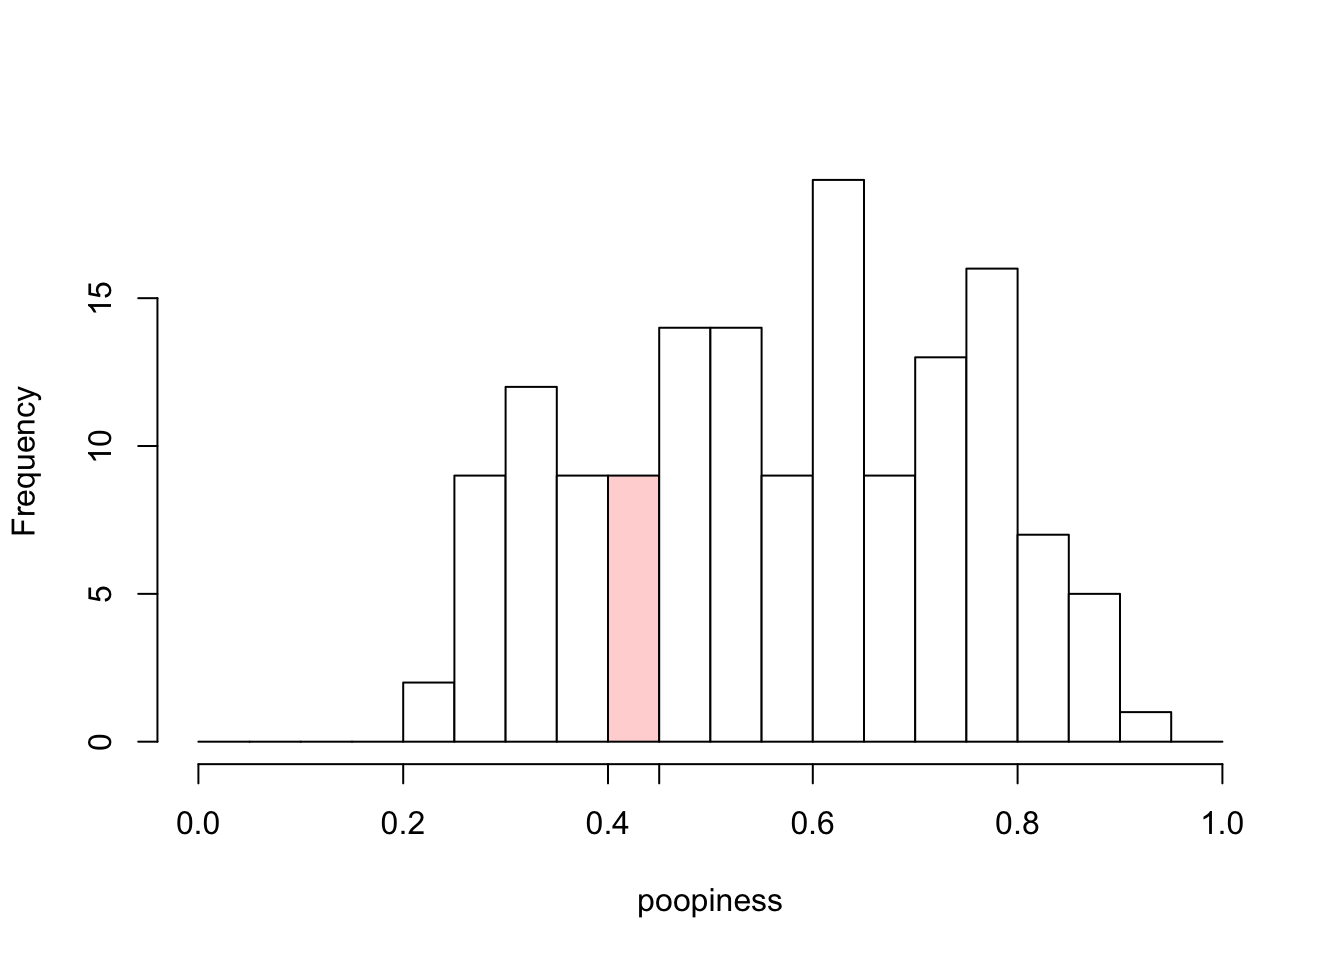
\includegraphics[width=0.9\linewidth]{carpedatum_files/figure-latex/poopy-hist-1} 

}

\caption{Histogram of Poopiness}\label{fig:poopy-hist}
\end{figure}

A histogram is a bar plot of counts for values that fall into certain numerical ranges. So it's a bar plot of the data in Table \ref{tab:poopy-freq}. But oftentimes you'll just see the histogram without the frequency table. It is worth noting that the information contained in the frequency table is equivalent to the information contained in the histogram, but it is sometimes easier to get a general idea of what is going on in the data by looking at the histogram.

Consider the range of poopiness values from 0.40-0.45. Our data set has 9 values in this range, as you can see in Table \ref{tab:poopy-freq}, so the height of the bar above this range of values on the x-axis (horizontal axis) is 9. I've colored it in pink only to help you see what I'm referring to. The y-axis in Figure \ref{fig:poopy-hist} is labeled ``Frequency'', as in the table. Some more jargon: the numerical values that separate the bins are called ``breaks.'' In Figure \ref{fig:poopy-hist}, the breaks occur are at increments of 0.05.

\begin{quote}
Question: Given that there are 20 possible bins in the histogram in Figure \ref{fig:poopy-hist}, but only some of them have non-zero counts, are there 20 kinds of people (in terms of poopiness) or 15 kinds of people?
\end{quote}

Trick question? You bet. The breaks (and thus bins) in a histogram are arbitrary. I can choose any breaks I want, as long as all of the data points fall into exactly one bin. (I can't just exclude some bins, though. That would be cheating.) The histograms in Figure \ref{fig:poopy-hist-alt} are both perfectly valid histograms. One of them has four bins, and one of them has only two bins.

\begin{figure}[H]

{\centering 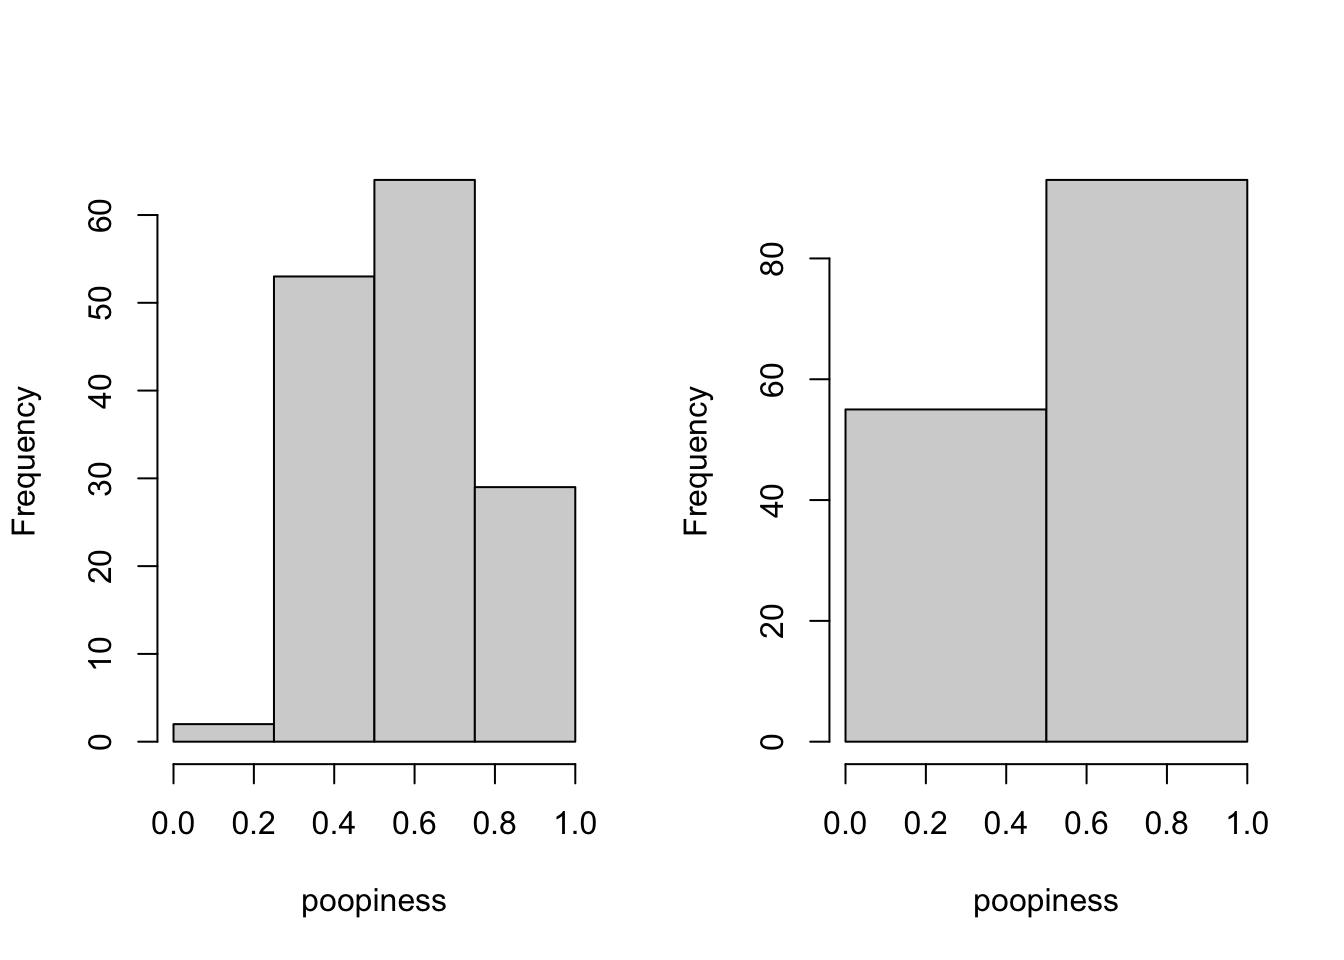
\includegraphics[width=0.9\linewidth]{carpedatum_files/figure-latex/poopy-hist-alt-1} 

}

\caption{Other Histograms of Poopiness}\label{fig:poopy-hist-alt}
\end{figure}

It's tempting to take the counts on the right of Figure \ref{fig:poopy-hist-alt} and declare that there are two kinds of people. After all, this gets us back to familiar territory. Ta-dah!

\begin{figure}[H]

{\centering 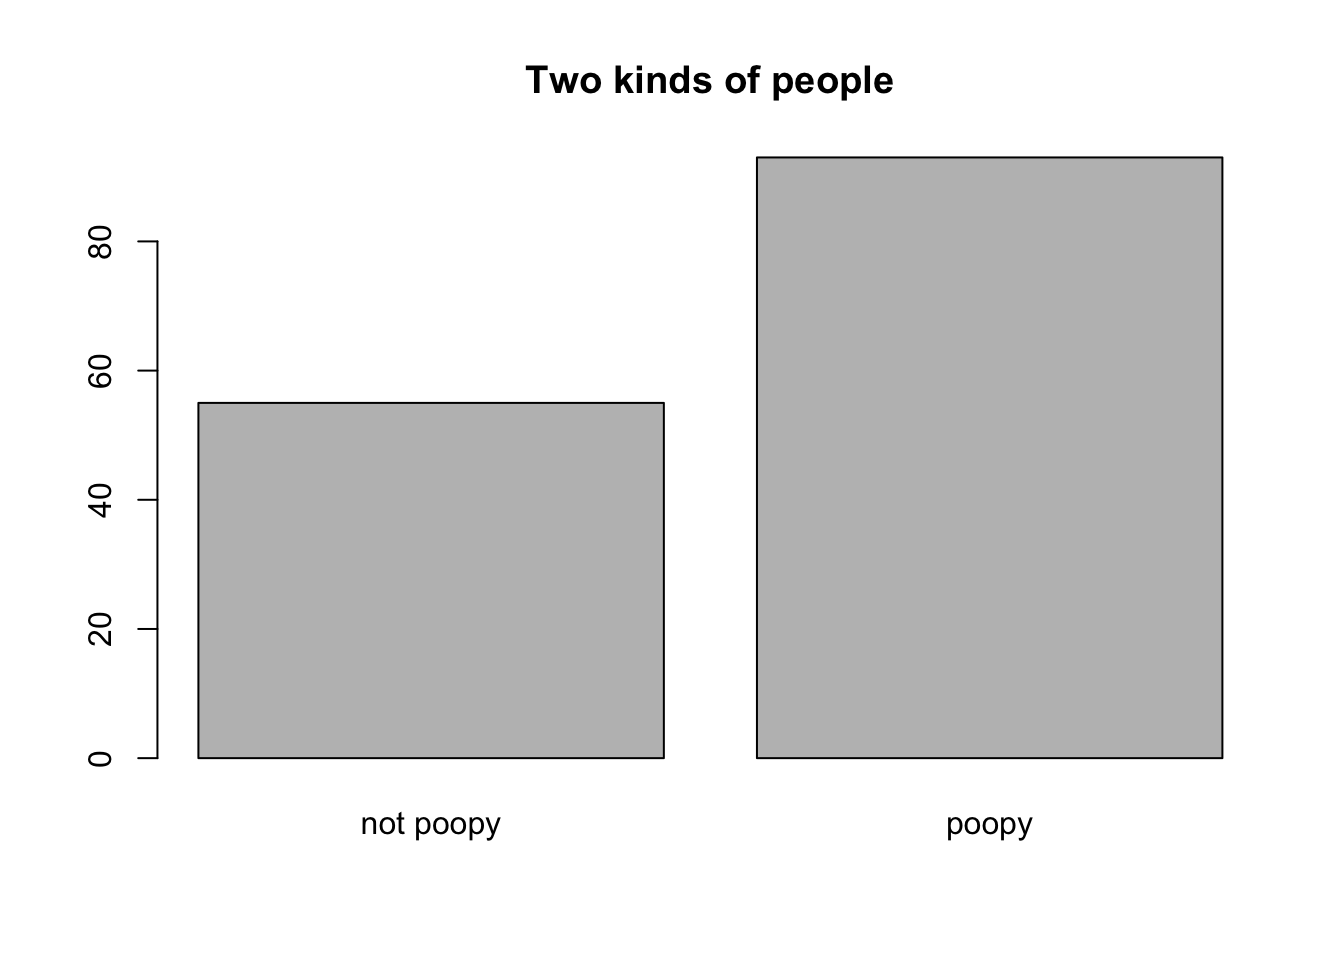
\includegraphics[width=0.9\linewidth]{carpedatum_files/figure-latex/poopy-two-kinds-1} 

}

\caption{This is a terrible, horrible, no-good, very-bad thing to do.}\label{fig:poopy-two-kinds}
\end{figure}

As you can tell, because it says so right in the figure caption, this is terrible, horrible, no-good, very-bad thing to do. Why do you think it is a bad thing to do? Choose one:

\begin{enumerate}
\def\labelenumi{\alph{enumi})}
\tightlist
\item
  The split was made at 0.5 on the poopiness scale, but that is not the average value of poopiness in the data set, which is closer to 0.57, as can be seen in Figure \ref{fig:poopy-hist} (or from the ``raw'' data themselves).
\item
  You should always use at least 5 bins when you have numerical data
\item
  Representations of data should communicate honestly about the nature of the data themselves. In this case, poopiness is not a category.
\end{enumerate}

What I did here was take a numerical/quantitative value (poopiness) and mis-represent it as a categorical value. I did it by \emph{dichotomizing} it, i.e., by splitting off everyone above 0.5 and labeling them as ``poopy''. I could have alternately split at the mean or median value and labeled the resulting two groups as ``low poopiness'' and ``high poopiness.'' But this would still have been a mis-representation. It would hide the fact that poopiness comes in a continuous range of values.

\begin{quote}
ASIDE (\emph{delivered in a hushed voice}): I won't be able to convince you of this now, but it turns out that if you do this---if you dichotomize numerical data---you will BREAK STATISTICS! Ok, that sounds a bit dramatic. But in all seriousness, one of the jobs of statistics is to understand associations between different variables, such as poopiness and, say, earning potential. If you treat poopiness (or other variables) as discrete when they are really continuous, you may very well get the wrong answers. As the man down the street from where I used to live often muttered to himself while waving his arms in the air, THAT IS AN ABSOLUTE IRONCLAD MATHEMATICAL FACT. No, but in all seriousness, there is a very good paper on exactly this subject \citep{maccallum2002}.
\end{quote}

Dang it! you say. You've taken me down this rabbit hole of poopiness for too long. How many kinds of people are there? Are you saying that if one looks at properties that are described by numbers instead of categories, that are no kinds of people at all? Is it all just shades of gray (or brown)?

\hypertarget{mixtures}{%
\subsection*{Mixtures}\label{mixtures}}
\addcontentsline{toc}{subsection}{Mixtures}

Remember Figure \ref{fig:poopy-hist}? (Don't click it!) Here it is again so you don't have to scroll back. Data scientists like to say this picture shows you the \textbf{distribution} of poopiness in our sample. Statisticians use the word distribution in a more formal way that is best put off until we actually need it. We don't need it yet.

\begin{center}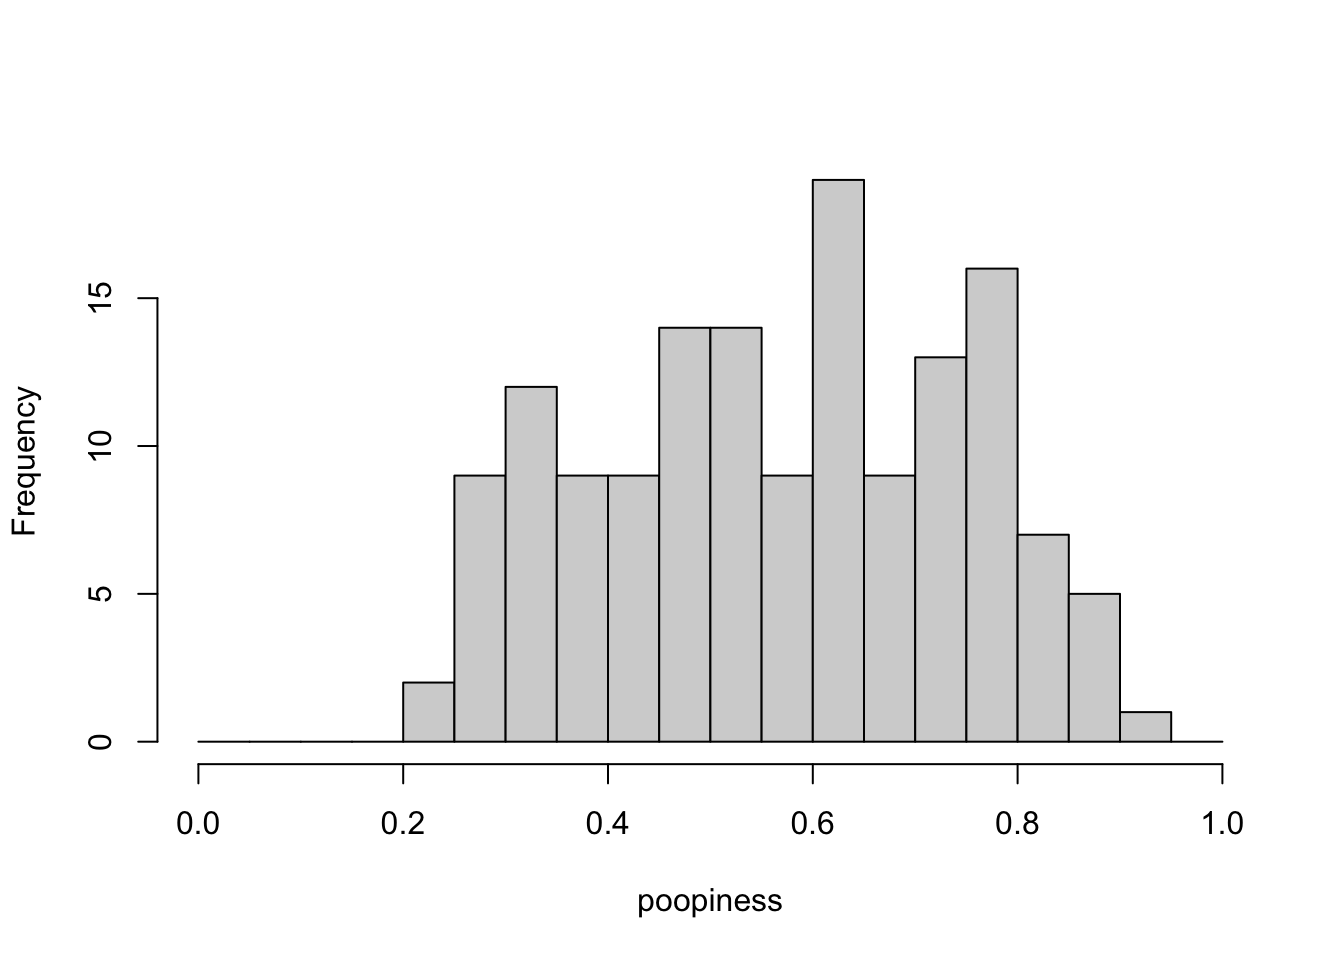
\includegraphics[width=0.9\linewidth,]{carpedatum_files/figure-latex/poopy-hist2-1} \end{center}

What if I told you that there ARE two kinds of people; you just can't see them unless I give you special glasses (or more information). If I gave you special glasses (or information), you would see this:

\begin{figure}[H]

{\centering 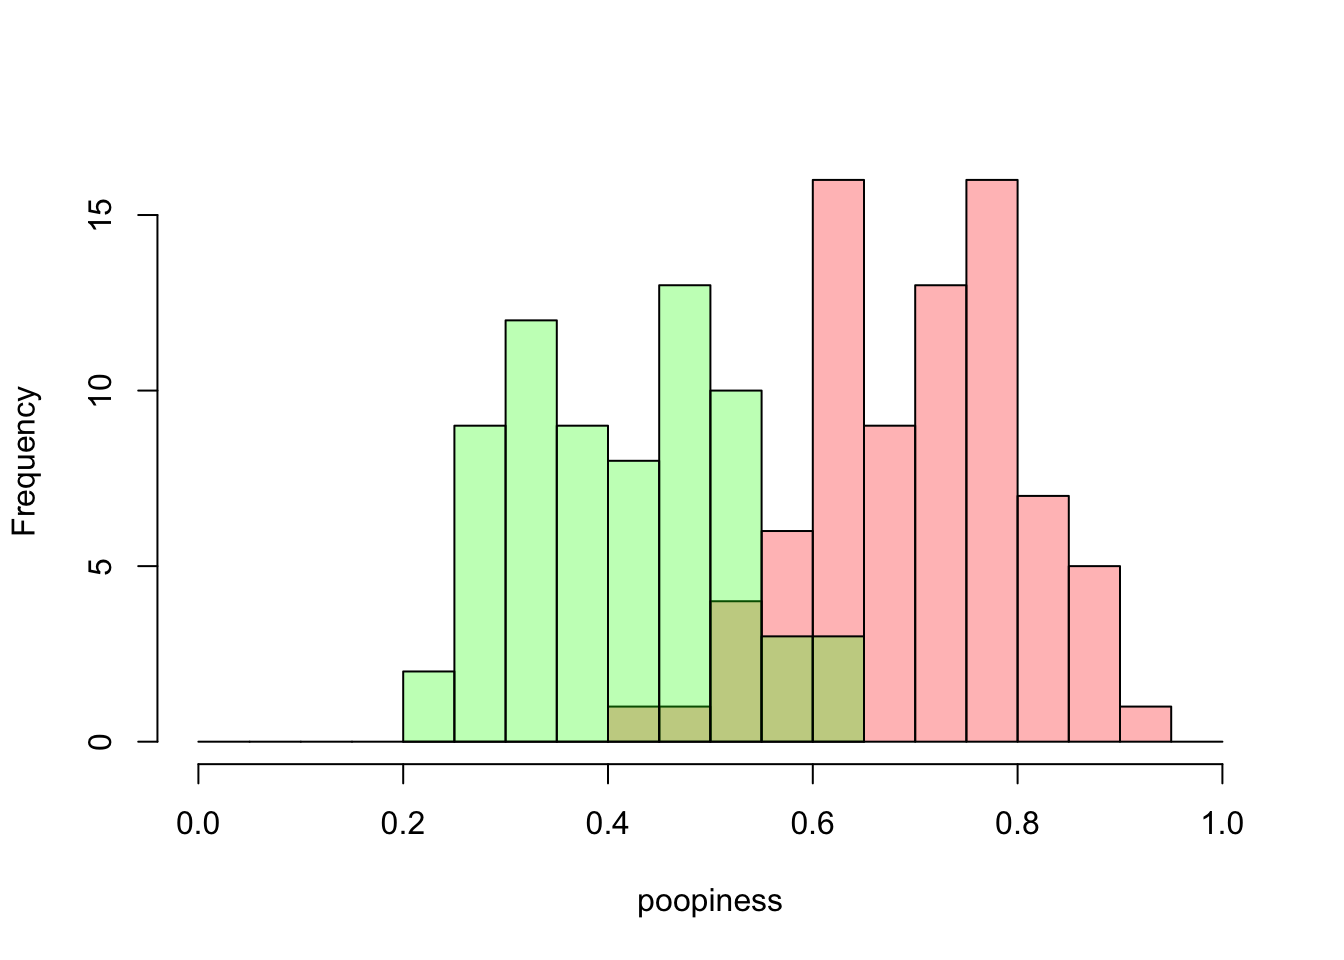
\includegraphics[width=0.9\linewidth,]{carpedatum_files/figure-latex/poopy-hist-mixture-1} 

}

\caption{A mixture of poopiness}\label{fig:poopy-hist-mixture}
\end{figure}

\emph{By what dark magic have you colorized the data!} you say. Or, perhaps you just said, hm, interesting.
In Figure \ref{fig:poopy-hist-mixture}, I've made a histogram with bars in two different colors, light green and pink. The colors are slightly transparent so that you can see both the green and pink distributions in their entirety even though they overlap. That's what the brownish bars mean. You're looking at the overlap of the green and pink bars, not another set of bars. Now, if you compare this histogram closely with the original, colorless histogram above, you'll see that the bin ranges are the same (width=0.05), and the the counts of green and pink bars add up to the total values that we had before. If there are green people and pink people, or in any case two different kinds of people, and if their poopiness is distributed as shown in Figure \ref{fig:poopy-hist-mixture}, then the poopiness of the mixture of these two groups of people will look just like Figure \ref{fig:poopy-hist}.

Ok, but that doesn't explain how you would know that there are two groups. If I didn't tell you. That's because \emph{you wouldn't necessarily know. You would need to have more information}. Now you might suspect something if you saw a distribution that looked like this:

\begin{figure}[H]

{\centering 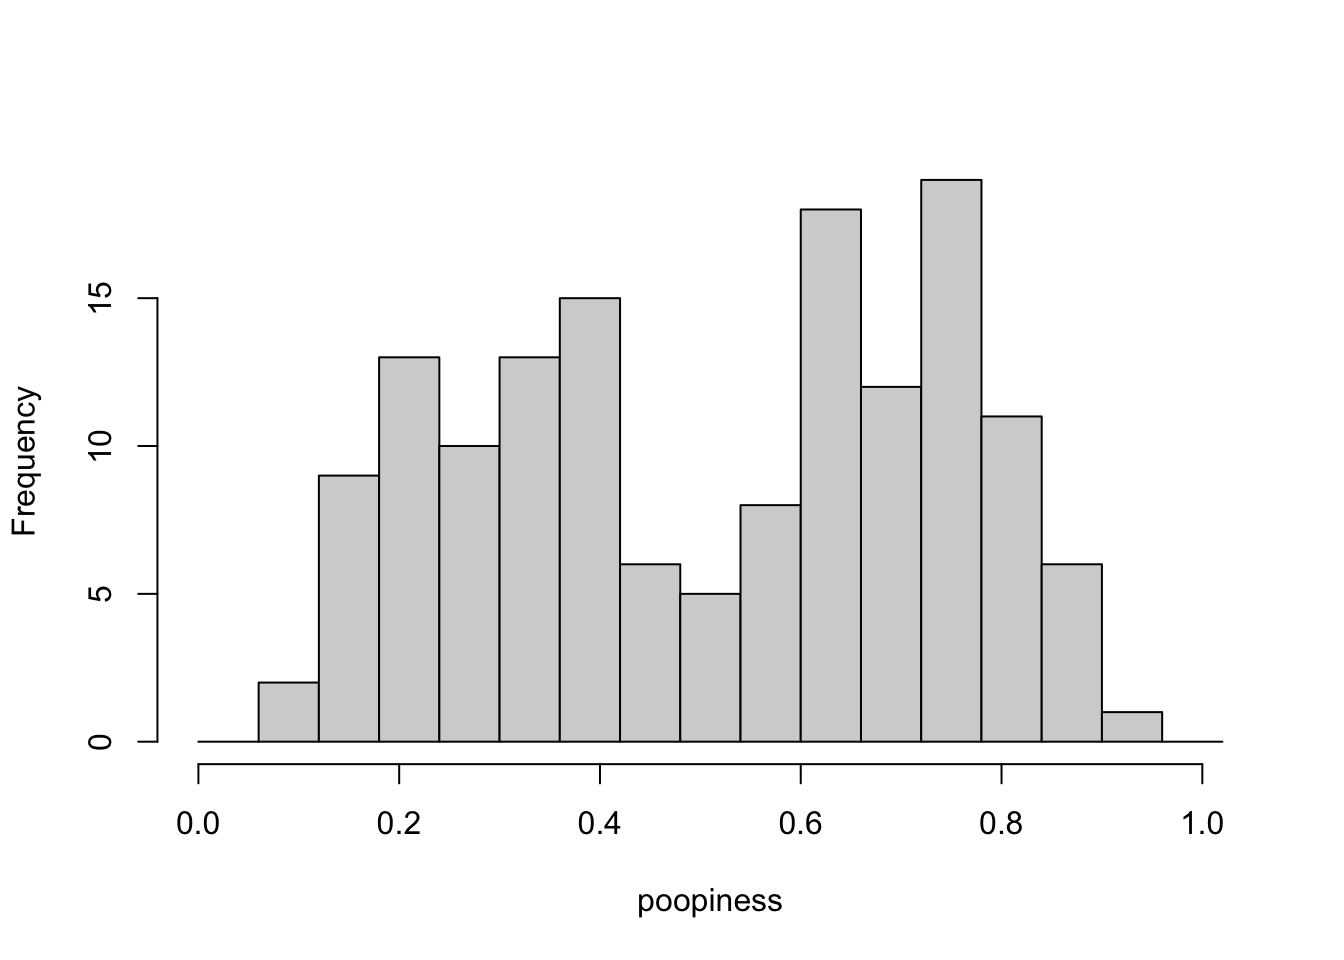
\includegraphics[width=0.9\linewidth,]{carpedatum_files/figure-latex/poopy-hist-mixture-suspicious-1} 

}

\caption{A suspicious mixture of poopiness}\label{fig:poopy-hist-mixture-suspicious}
\end{figure}

In Figure \ref{fig:poopy-hist-mixture-suspicious}, the distribution has a double-hump like a Bactrian camel. In spite of that, it is not called a Bactrian distribution--which would make me happy--but a \textbf{bimodal} distribution. The point that I'm trying to make here is that a bimodal distribution makes you suspect that there could actually be (at least) two groups mixed together in our data.

But the original data for poopiness did not look bimodal. I suggested to you that you would need more information to determine if there are two groups. And so, I present you with\ldots{} Crappiness!

\hypertarget{crappiness}{%
\section*{Crappiness}\label{crappiness}}
\addcontentsline{toc}{section}{Crappiness}

For each of the subjects in our poopiness data set, we have also collected data on their crappiness. Crappiness is also reported as a numerical value ranging from {[}0,1{]}. It's sort of like poopiness, but different. Here are some values:

\begin{verbatim}
##      poopiness crappiness
## 0040     0.319      0.564
## 0140     0.703      0.415
## 0033     0.401      0.729
## 0107     0.544      0.374
## 0031     0.538      0.853
## 0100     0.657      0.316
\end{verbatim}

And here\ldots(drum roll please)\ldots{} is a histogram of crappiness!

\begin{figure}[H]

{\centering 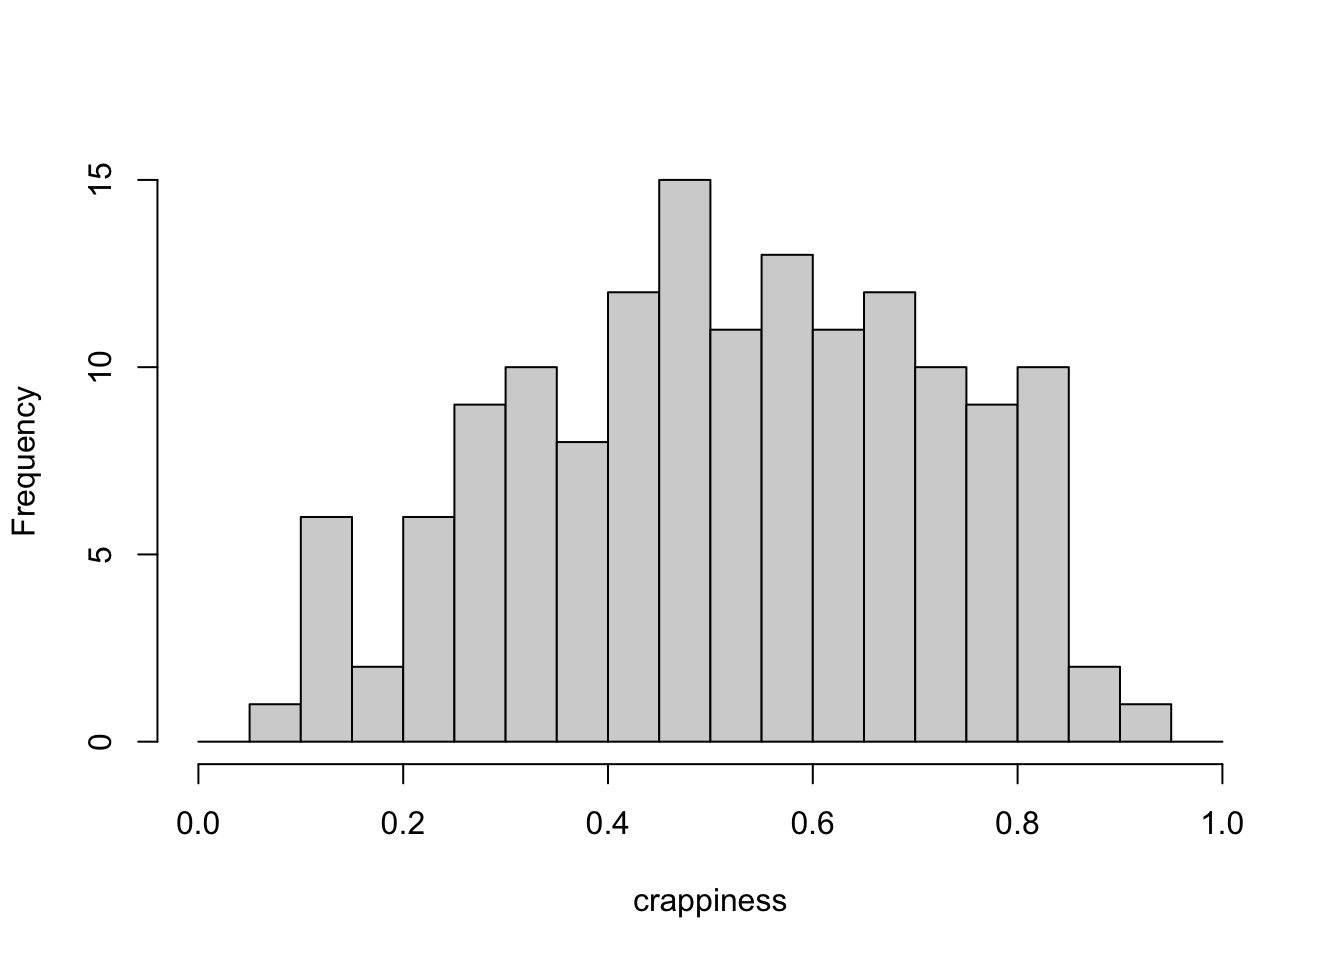
\includegraphics[width=0.9\linewidth,]{carpedatum_files/figure-latex/crappy-hist-1} 

}

\caption{Histogram of Crappiness}\label{fig:crappy-hist}
\end{figure}

Hmm. I bet you were hoping that the crappiness data would look obviously bimodal, but it's not obvious. Nevertheless, hopefully you trust that I wouldn't lead you on a wild goose chase for no reason. Perhaps you can even see it coming. If we look at poopiness and crappiness separately, there is no clue that there might be distinct groups of people in our data set. But if we look at them together\ldots{} there is.

When we looked at categorical data for two two-kinds-of-people questions, we made 2x2 contingency tables. We also used the word ``dimension'', for example to say that we were describing people along two dimensions (recall: toilet paper and peanut butter). Now that we are looking at numerical data (poopiness and crappiness), we can also use two dimensions, as in a two-dimensional scatterplot, to examine both variables at once.

A scatterplot is just a name for a data plot, in which the position of each data point corresponds to its coordinates along more than one dimension. We often refer to two-dimensional coordinate systems as (x,y), where x is the horizontal axis and y is the vertical axis. Technically, in this case our coordinate system is (poopiness, crappiness). These are the names of our dimensions. But we will still often refer back to the idea of an x- or y-axis. This scatterplot is shown in Figure \ref{fig:poopy-crappy}. Each point represents data from one person, with their poopiness value on the x-axis and crappiness on the y-axis.

\begin{figure}[H]

{\centering 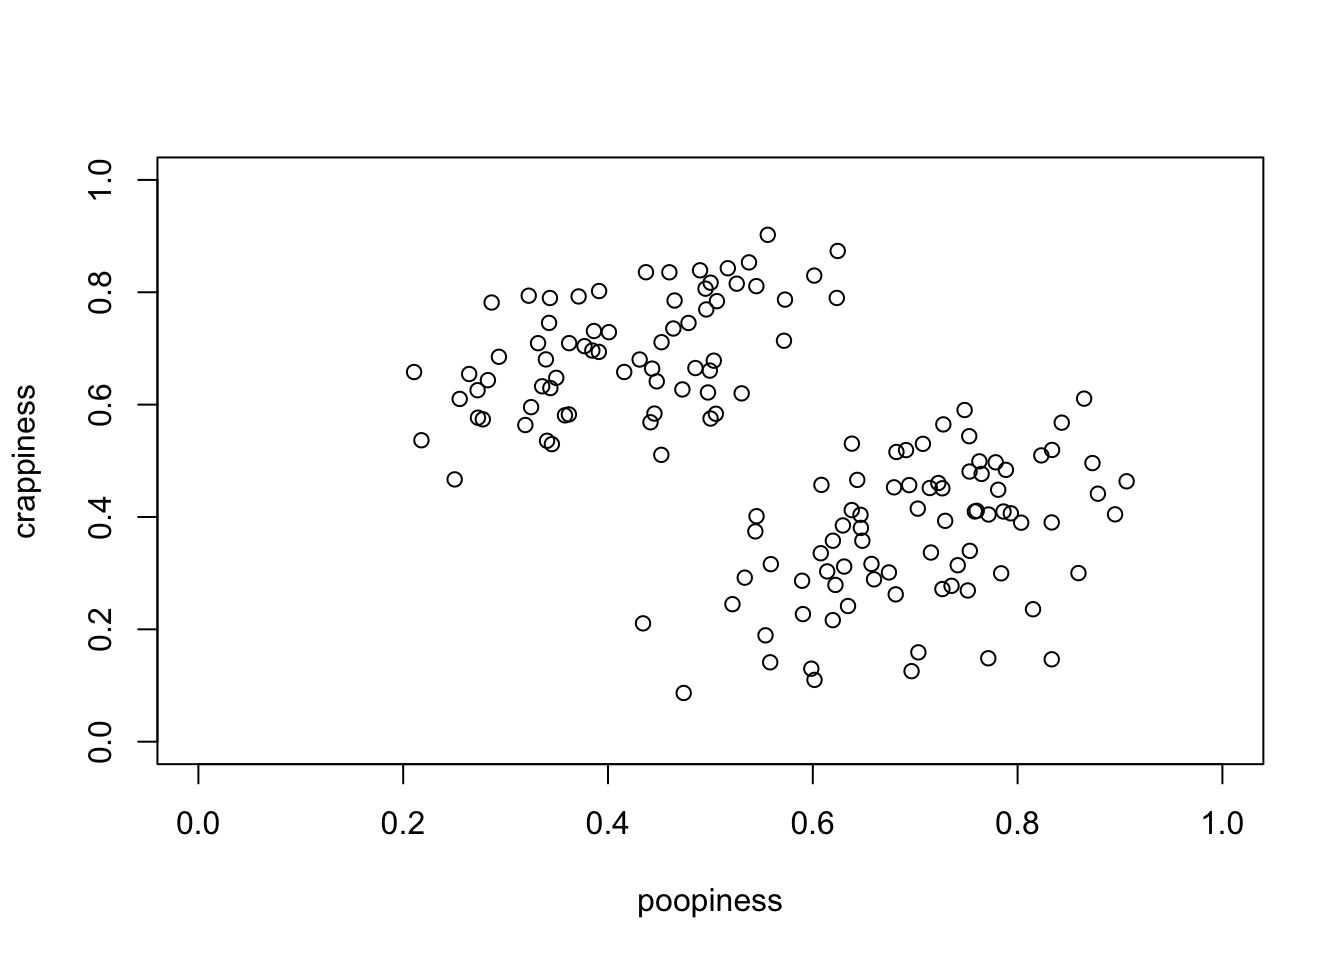
\includegraphics[width=0.9\linewidth,]{carpedatum_files/figure-latex/poopy-crappy-1} 

}

\caption{Scatterplot of Crappiness vs Poopiness}\label{fig:poopy-crappy}
\end{figure}

Alas, oh data! Your bimodal nature has revealed itself in the higher-dimensional plane!

How many kinds of people are there? When it comes to poopiness and crappiness, people exhibit a continuous range of values, so we can't neatly put them into buckets. Neither poopiness nor crappiness appear to be bimodally distributed on their own. However, when examined together, as in the scatterplot in Figure \ref{fig:poopy-crappy}, a pretty suggestive pattern emerges in the data. There are two \textbf{clusters} of points, one group of which is lower in poopiness but higher in crappiness than the other. Interestingly, though, in both groups poopiness and crappiness tend to increase together. That is, they appear to be associated, not independent.

I do not mean to imply that clusters of points can always be found if we have data along many dimensions. That is certainly not always the case. The present example was concocted (I admit it!) to show that groups \emph{can} emerge, even in numerical data. Cluster analysis \citep{kaufman2009} refers to set of data-science methods all about looking for the existence of groups in multidimensional data.

\hypertarget{check-your-understanding}{%
\subsection*{Check your understanding}\label{check-your-understanding}}
\addcontentsline{toc}{subsection}{Check your understanding}

\begin{enumerate}
\def\labelenumi{\arabic{enumi})}
\tightlist
\item
  Based on the scatterplot in Figure \ref{fig:poopy-crappy} and the grouped-by-color histogram for poopiness in Figure \ref{fig:poopy-hist-mixture}, describe what the equivalent grouped-by-color histogram for crappiness would look like. Would it look the same or different? Explain.
\end{enumerate}

\hypertarget{cut-scores-and-abnormality}{%
\chapter{Cut Scores and Abnormality}\label{cut-scores-and-abnormality}}

\begin{quote}
Because that's not what normal people do.
--- things my spouse says
\end{quote}

You'll recall that I previously warned against possible negative consequences of setting arbitrary cut points to dichotomize a data set---that is, turning numerical data on a continuous scale into two categories by using a cutoff value. But now consider the following scenarios:

\begin{enumerate}
\def\labelenumi{\arabic{enumi})}
\item
  To pass the written test for your a driving learner's permit in California, you must answer at least 38 questions correctly out of 46. That's 82.6\% correct. At 80.4\% (37/46) or below, you fail and have to retake the test on another day.
\item
  A patient's blood test shows levels of ALT (alanine aminotransferase) at 77 units per liter. The lab report labels this as ``abnormally'' high, and the physician is concerned about possible liver damage or disease.
\end{enumerate}

These two examples involve just the kind of dichotomization that I cautioned against, and yet they occur very commonly in practice. So what gives? Is it wrong to use cutoffs this way? Why do people do it?

The short answer is that we often find ourselves in need of a classification (pass or fail; diagnose liver disease or not) but without a perfect classification device. Rather we have only indirect measurements (of knowledge or liver function) in some quantitative measure. Perhaps you once found yourself on the ``border'' between letter grades for a course and were particularly perturbed (or relieved) by the imperfections of such a system. Or you may have found yourself with ``slightly'' abnormal levels in a blood test and wondered whether you should seek further tests.

Both the California department of motor vehicles and the physician in our scenarios need to make a decision based on imperfect evidence. They want to be able to say that the person's test results show that they are ready to get behind the wheel of a car, in one scenario, or suffering from liver problems in the other. But all they can really do is express this belief using a \textbf{probability}. This probabilistic judgement is based on a mathematical \textbf{model} that relates traits like readiness-to-drive or liver-disease to certain test results. Understanding how these models come into existence is one of the learning objectives of this course.

The term \textbf{normal distribution} arose in statistics because the particular bell-shaped distribution occurs so frequently. If poopiness were normally distributed in our sample from before it might look like this.

\begin{figure}[H]

{\centering 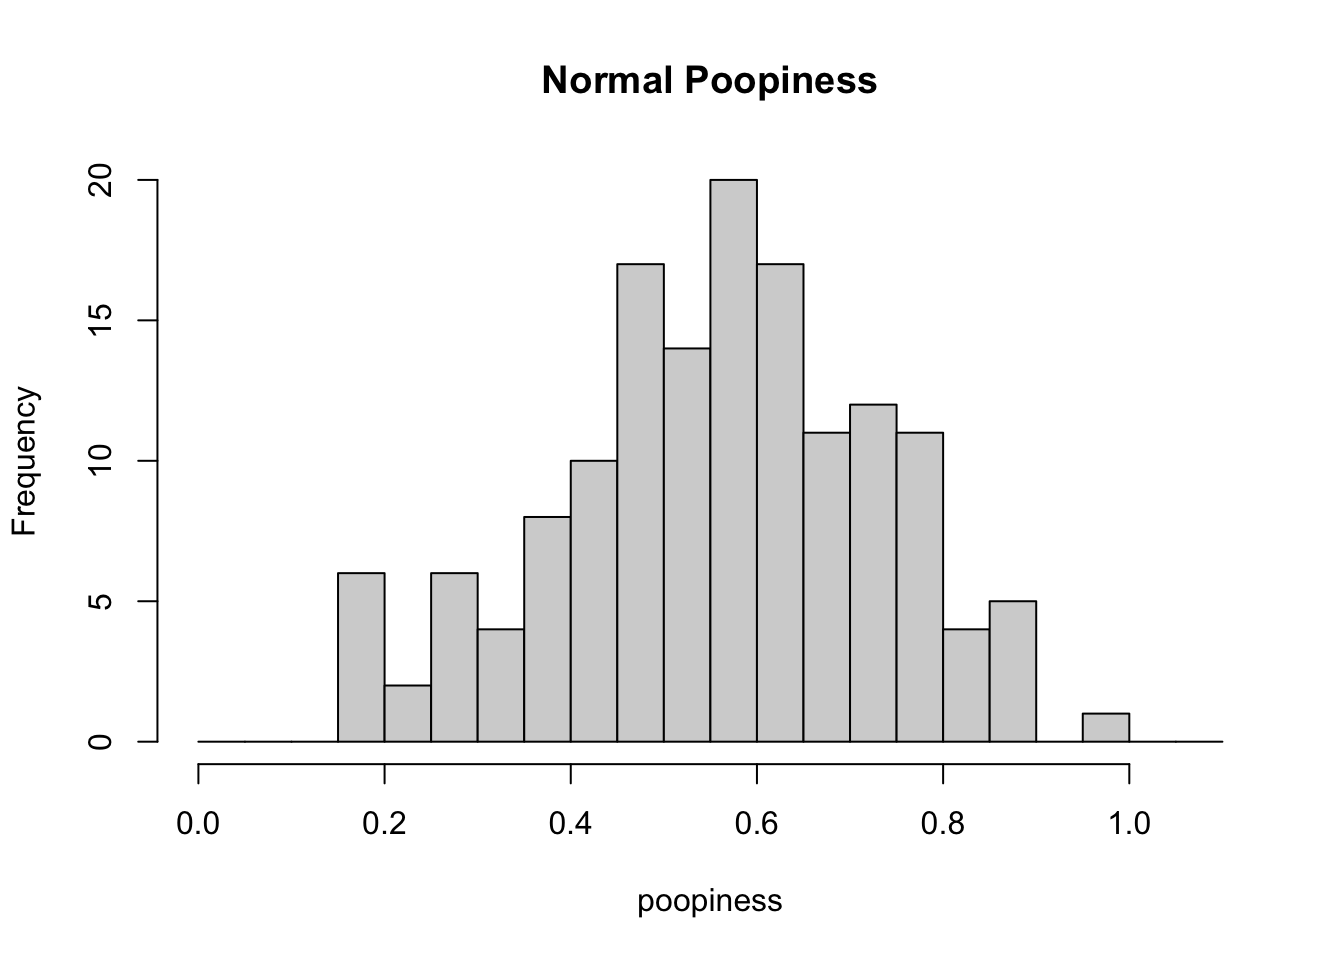
\includegraphics[width=0.9\linewidth,]{carpedatum_files/figure-latex/normal-poopy-1} 

}

\caption{Normal poopiness}\label{fig:normal-poopy}
\end{figure}

Technically speaking, all of the values, including the maximal value of 0.962 that we observe in Figure \ref{fig:normal-poopy} are normal. Poopiness varies in the population. It is impossible to be abnormally poopy, under the circumstances. By definition, some values at the extreme ends of a normal distibution are less likely to occur than values in the middle. But still they may occur rarely. It is only when extreme values (large or small) are associated with other conditions of interest, such as the relationship between elevated ALT and liver disease, that it makes sense to ``flag'' these extreme values.

We say that we \textbf{discretize} continuous variables (i.e., turn them into discrete categorical variables) by using thresholds or cut scores. Passing a test or being flagged for liver disease is usually based on a single cut score. The cut score is a numerical value, and data that fall above or below that value are categorized differently. It is possible to use more than one threshold. For example, in the next chapter we will see that people can be classified as belonging to different generations based on their age, and neighborhoods can be categorized based on their population density.

We started out this course on a quest to answer our first big question: How many kinds of people are there? En route, we have examined both categorical data, such as from two-kinds-of-people questions, and numerical values like poopiness. The toilet paper and peanut butter orientation questions may seem silly and inconsequential to you. I can only imagine what you might think of the poopiness and crappiness dimensions that I completely made up (I admitted it!). However, in the next chapter we will see how some more standard variables are used to profile American people. Next week, we will see more issues of discrete/categorical and continous/numerical multi-dimensional descriptions of people that arise when it comes to personality psychology.

\hypertarget{remember-these-terms}{%
\subsubsection*{Remember these terms?}\label{remember-these-terms}}
\addcontentsline{toc}{subsubsection}{Remember these terms?}

\begin{itemize}
\tightlist
\item
  kind, type, category
\item
  discrete, continuous, numerical, dichotomous
\item
  crosstab, two-way table, contingency table
\item
  association, contingency, dependence
\item
  latent factor, dimension, trait
\item
  measurement, model, histogram, bimodal, cluster
\end{itemize}

\hypertarget{the-modal-american}{%
\chapter{The Modal American}\label{the-modal-american}}

The NPR podcast Planet Money aired an episode in the summer of 2019 called \href{https://www.npr.org/2019/08/28/755191639/episode-936-the-modal-american}{The Modal American}. If you haven't listened to it, you should stop what you're doing and listen to it right now. (Seriously, this will make a lot more sense).

The podcast hosts, Kenny Malone and Jacob Goldstein, set the stage as follows. People sometimes talk about the ``average'' American, but that doesn't really make sense, even as an idea. If you average the traits of all Americans, you don't end up with a real human being.\footnote{We encountered this fact in the form of a joke in Chapter \ref{categories}, specifically \protect\hyperlink{no-mean-feat}{here}} Malone suggests that what people are really thinking about is the \emph{modal} American, i.e., the most common type of American. The kind person you're more likely to bump into on the street than any other. The hosts then consult with economics and data reporter Ben Casselman to help identify who is the modal American.

For the purposes of their investigation, the kinds of American the Planet Money hosts are interested in are determined by groupings of demographic variables like those collected by the US Census. The census does not, to my dismay, include questions about peanut butter preference, toilet paper orientation, digitidiness, or poopiness. Rather, they stick with things like sex, race, age, income, marital-status, etc. It turns out that different people mean different things when the ask, ``how many kinds of Americans are there?'' In any case, this journey to put Americans into buckets leads down some paths that will be very familiar to you by now.

\hypertarget{step-one-categories}{%
\subsection*{Step one: categories}\label{step-one-categories}}
\addcontentsline{toc}{subsection}{Step one: categories}

First of all, some of the variables, like sex, race, and marital status, are categorical to begin with. We can ask people to answer these survey questions, and then we can combine their answers into kinds like married-Hispanic-male or \href{https://www.imdb.com/title/tt0105414/}{single-White-female} types of people.

Some of the variables included, like neighborhood-type, are categorical in the way we think about them (read: rural, suburban, or urban), but are actually derived from numerical variables. In this case, neighborhood type is derived from the population density in the census block. Other variables, like income and, arguably, age, are just plain numerical. But to identify the most common kind of American, our podcast hosts need to put people into categories (like rich and poor--to make things dichotomous--or low-, middle-, and high-income). So they \textbf{discretize} all of the numerical variables into a small number of categories. They ``bin'' the incomes as well as the ages, which they combine into generation labels like ``Generation X'' and ``Baby Boomers.''

\hypertarget{step-two-contingency-table}{%
\subsection*{Step two: contingency table}\label{step-two-contingency-table}}
\addcontentsline{toc}{subsection}{Step two: contingency table}

Having done all this, the next step is to combine the data about all Americans along each of these variables into one big contingency table. It's not a two-way table, because there are more than two variables, but it's still a contingency table. (It is not very common to use terms like four-way or five-way table.)

The choice of variables, and specifically the choice of the number of categories to keep for each one, determines how many kinds of Americans there can be. Having made the choices, it is a simple matter of looking to see which is the most common kind.

Along the way, the idea of dependence, or association, also comes up, but it is not necessarily mentioned by name. Supppose you know the most common age category is Children. And suppose the most common category of marital-status is Married. It does not necessarily follow that married-children is the most common category in a two-way table made from those two variables. Of course, the opposite is true. And this is because age and marital status are associated variables. The older you are, the more likely you are to be (now or previously) married, as opposed to never married. In general, you cannot assume that the most common category in two variables will combine to produce the most common two-variable-category. \textbf{But this would be true if the variables were independent.}

For independent variables, it must be the case that the most common joint category will emerge from the simple combination of the most common individual categories. You could actually use that as a definition of independence.

Take sex and race, for example. In the Planet Money podcast, both of these are actually treated as dichotomous variables (all race categories other than white are combined into one, so it is basically white or not; perhaps you are hearing ``there are two kinds of people in this world\ldots{}''). Since female is the most common sex and white is the most common race category, it has to be the case that white-female comes out as the most common combination. Sex and race are independent.

Perhaps it is reassuring to you that the ideas we have been developing are not just limited to semi-jokey two-kinds of people questions, or Buzzfeed personality tests. But that they apply exactly as before to serious data.

\hypertarget{exercises}{%
\subsection*{Exercises}\label{exercises}}
\addcontentsline{toc}{subsection}{Exercises}

\begin{enumerate}
\def\labelenumi{\arabic{enumi}.}
\tightlist
\item
  At around minute 5:15, the hosts describe the what they see looking at the (histogram of) age distribution. What kind of distribution are the hosts describing?
\item
  Why such (over)simplification? Hint: there is a discussion around 9 minutes in.
\item
  The methodology of the Planet Money analysis is described on \href{https://www.npr.org/2019/08/28/755191639/episode-936-the-modal-american}{their website}. From this, determine how many variables there are, how many categories there are for each one, and thus how many kinds of Americans (i.e., how many buckets) there are in total.
\end{enumerate}

\hypertarget{sixteen-personalities-or-five-factors}{%
\chapter{Sixteen Personalities or Five Factors?}\label{sixteen-personalities-or-five-factors}}

Before you read this chapter, you might want to go ahead and take one of the personality tests based on
the Meyers-Briggs Type Indicator (MBTI) categories and/or the five-factor model of personality (also called the Big Five). There is only one ``official'' MBTI, which is a commercial product. However, there are several free alternatives online which use the same typology classification. There are also several variations of the Big Five.

\begin{quote}
Test yourself:

\begin{itemize}
\tightlist
\item
  MBTI-style at \url{16personalities.com} or

  \begin{itemize}
  \tightlist
  \item
    \url{https://openpsychometrics.org/tests/OEJTS/}
  \end{itemize}
\item
  Big Five

  \begin{itemize}
  \tightlist
  \item
    \url{http://www.personal.psu.edu/~j5j/IPIP/}
  \item
    \url{https://bigfive-test.com/}
  \item
    \url{https://openpsychometrics.org/tests/IPIP-BFFM/}
  \item
    General information about these test items: \url{https://ipip.ori.org/}
  \end{itemize}
\end{itemize}
\end{quote}

I will only minimially describe the MBTI and the Five Factor Model (FFM, or Big Five) here, in terms of the topics we have been discussing. There are many resources for learning more about these personality tests. Some are referenced under further reading.

\hypertarget{mbti}{%
\subsection*{MBTI}\label{mbti}}
\addcontentsline{toc}{subsection}{MBTI}

The MBTI will categorize people, based on their responses, dichotomously along each of four dimensions, also called ``scales.'' These are:

\begin{itemize}
\tightlist
\item
  Extraversion-Introversion (E-I)
\item
  Sensation-Intuition (S-N)
\item
  Thinking-Feeling (T-F)
\item
  Judging-Perceiving (J-P)
\end{itemize}

Thus there are sixteen possible combinations, for example ``INTP''. Each person is assigned to one of these sixteen personalities. Many online tests will provide you with a report to help interpret your classification. That is, the four dimensions are understood to come together in some holistic picture of your ``type.''

\hypertarget{big-five}{%
\subsection*{Big Five}\label{big-five}}
\addcontentsline{toc}{subsection}{Big Five}

The term ``Big Five'' is a commonly used term for the five-factor model of personality. Based on responses to questionnaires, people are assigned a numerical score along five dimensions (also called scales or factors!)

\begin{itemize}
\tightlist
\item
  Neuroticism refers to the tendency to experience negative feelings.
\item
  Extraversion is marked by pronounced engagement with the external world.
\item
  Openness to Experience describes a dimension of cognitive style that distinguishes imaginative, creative people from down-to-earth, conventional people.
\item
  Agreeableness reflects individual differences in concern with cooperation and social harmony. Agreeable individuals value getting along with others.
\item
  Conscientiousness concerns the way in which we control, regulate, and direct our impulses.
\end{itemize}

\begin{quote}
Fun fact: both OCEAN and CANOE are mnemonic devices that can help you recall the names of the Big Five dimensions.
\end{quote}

Since the results of a Big Five test, such as the IPIP-NEO, are five numbers, you don't get assigned a personality ``type'' by these tests. Rather, you may be provided with an explanation of what it means to score high (or low) on, say, Extraversion. You may have noticed that extraversion (occasionally spelled ``extroversion'') appears on both the MBTI and the Big Five.

\hypertarget{twenty-questions-about-extraversion}{%
\subsection*{Twenty Questions (about Extraversion)}\label{twenty-questions-about-extraversion}}
\addcontentsline{toc}{subsection}{Twenty Questions (about Extraversion)}

Suppose, for whatever reason, we want to identify a person's extraversion. We may want either (a) to classify them as extraverted or not (i.e., introverted), or (b) to quantify a degree of extraversion, say on a scale of 0-100. Why not then just pose the question in the following way? In the first case:

\begin{enumerate}
\def\labelenumi{\alph{enumi})}
\tightlist
\item
  Choose the one that describes you: Extraverted ~~~~\textbar{} ~~~~Introverted
\end{enumerate}

or, in the second case,

\begin{enumerate}
\def\labelenumi{\alph{enumi})}
\setcounter{enumi}{1}
\tightlist
\item
  Locate yourself on the scale: Extraversion 0 . . . . 50 . . . . 100
\end{enumerate}

Personality tests, such as those we've discussed above, do not ask questions like these. Rather, they include many different questions, sometimes twenty or even more, about things like going to parties, making friends, and drawing attention to oneself. Why ask twenty questions instead of just one?

Recall from the great toilet paper debate that it was not necessary to ask twenty questions to know whether you were an over-hanger or an under-hanger. However, when we discussed digitidiness, we suspected that two different questions may have both been getting at the same latent factor. The situation here, in the real-life domain of personality testing, is similar.

\begin{tipblock}
\textbf{Golda asks}: So the idea is to design questions that are smarter than the user? Do we not trust people's abilities to self-categorize? Maybe these tests would be more effective if they allowed people to draw their own conclusions about themselves?

\textbf{Sidney says}: Developers of these questionnaires acknowledge that it is not as easy for people to self-categorize (what do you really mean by introverted? is that a bad thing?) as it is to describe how they feel at parties. Furthermore, category labels may seem socially desirable to the respondent, leading them to make a certain choice for ``appearances.'' So, to some extent yes, psychologists may not always trust people to self-categorize. But I think they would still defend everyone's right to draw their own conclusions from the results of a personality test.

\end{tipblock}

Psychologists \sout{believe that extraversion is an underlying factor} invented the idea of extraversion to explain patterns of behavior, including patterns of responses to questions about how people feel in various situations. Such as enjoyment or lack thereof in being the center of attention. The use of indirect evidence such as questionnaire responses to make inferences about psychological traits is the main task of \textbf{psychological measurement} (also called psychometrics). The main challenge of psychological measurement, perhaps even the reason for its existence as a method and field of study, is that human beings are noisy.

Put another way, you cannot expect a deterministic relationships between a person's response or behavior (how a person feels or acts) in one situation and how they respond or behave in another. Even someone we may want to call an extraverted person is not \emph{always} extraverted. And an extraverted person might not always answer questions about their feelings in the same way. It is also hard to directly observe extraversion or to ask people to simply self-report it. Extraversion manifests itself differently at different times and in different contexts. Whether this noise is due to some mysterious internal process, like a coin flip in your brain, or due to many unnaccountable external factors, like whether you slept poorly that day, we can't really say. What we can say is that human noisiness manifests itself as \textbf{measurement error} when we try to measure things like extraversion using questions and other observations.

Variability in human behavior is one of the factors that may contribute to measurement error. If the same person's behavior varies randomly over time, then our observations at any given time are subject to this variation. But we could also imagine having measurement error sources that come from ambiguously worded questions, which would still lead to errors even if behavior were stable. Say someone is asked if they engage in risky health behaviors. Even if their behavior is very consistent (for argument's sake), different people make have different perceptions of what counts as risky. So in that case measurement error results from (variation in) the interpretation of the question rather than from variation in risk-behavior over time.

The word \textbf{error} makes it sounds like there is a right answer, and that (personality) tests get it wrong. This is, indeed, one view (called true score theory in psychometrics). However, you don't have to believe that there is a right answer. For example, you can believe that human beings have some amount of inherent unpredictability. But just because human behavior is not perfectly predictable, just because observations are not deterministically related, we can still say that---in spite of measurement error---some patterns do remain. The responses to different questions about extraversion, for example, are associated with one another. People who say that they feel comfortable at parties are also likely to say that they make friends easily.

\hypertarget{but-whats-the-point}{%
\subsection*{But what's the point?}\label{but-whats-the-point}}
\addcontentsline{toc}{subsection}{But what's the point?}

Trying to describe people in terms of kinds or numerical scales is complicated. Why do we even bother? It's tempting to say that we just want to understand ourselves better, and that is certainly a reasonable answer. Sometimes, though, we want to predict how someone will act in the future, perhaps in a situation that differs from one that they have faced in the past. In that case, we can't exactly use the past to predict the future, unless we do so by making inferences about underlying traits from past behaviors and then predicting how someone with those particular traits would act in a new context. This purpose drives some uses of tests based on the MBTI and the Big Five, for example by employers or career counselors. However, although the MBTI is often used for these purposes, one should exercise caution in doing so \citep{pittenger1993}. You should certainly not assume that all personality tests do an equally good job of providing information for the desired inferences.

According to the standards of the American Psychological Association \citep{american1999}, whenever psychological tests are used for some specific purpose (e.g., employment, admission to a school or hospital, or even in court) there must be a valid argument for the intended purpose of the test scores. This \textbf{validation argument} will usually involve many facets, including how consistent the results of the test are, whether it is a fair test for all groups of people, whether test scores really are associated with relevant outcomes in the domain of use, and so on. These arguments, and challenges to them, are all part of what we mean by validity.

\hypertarget{recap-1}{%
\section*{Recap}\label{recap-1}}
\addcontentsline{toc}{section}{Recap}

So far, in pursuit of our question ``How many kinds of people are there?'', we have not been overly concerned with specific proportions or probabilities. Our discussion has been rather \emph{metaphysical}. We have tried to understand how differences that we observe among people can be expressed in terms of kinds (categories) or quantities (numbers), which are themselves different \emph{kinds} of data.

We have looked at dichotomous questions of both frivolous (toilet paper orientation or peanut butter preference) and less frivolous (attainment of Bachelors degree, employment status) kinds. Similarly, we've considered numerical variables from poopiness and crappiness to neuroticism and conscientiousness. We've seen that categorical questions can include more categories than two (e.g., peanut butter preference, if we include ``hate all'' and ``don't care'', but also ethnicity or neighborhood-type). We saw that numerical variables can sometimes be discretized and thus converted into categories, such as when income is classified as high or low, when age is converted to ``Generation Z'', or when a score on a personality test assigns you the value ``Perceiving'' as opposed to ``Judging.''

We saw that categorical questions can naturally classify people into types, and that when we combine different kinds of questions, the number of types/kinds/buckets can increase. But we also observed that the number of observed types does not necessarily increase to its mathematical maximum because answers to different questions can be associated. In other words, the number of factors or dimensions can be smaller than the number of questions. (But it can also be equal to the number of questions, in simple cases).

We also saw that numerical variables can be used to classify people. This can happen when we use cut-scores as thresholds and assign people above a threshold a value like ``pass'' or ``abnormal'' or ``introverted.'' The distribution of a numerical variable can be observed using a histogram, and sometimes a histogram is observed to have two bumps, which suggests a mixture of two different groups. But we also saw by plotting points on a coordinate plane of poopiness and crappiness that numerical data can cluster into groups, even when we don't see tell-tale signs of those groups along any single variable. The notion of clustering is all about identifying groups of data points that might designate types. According to some researchers, types can actually be recovered in the five-factor (Big Five) model of personality, which until recently was strongly thought of as \emph{not} having types.

You've probably figured out by now that this course is less about answering the Big Questions than about understanding how they might in principle be answered. What does one have to understand to even formulate an answer? Different people may indeed come to different answers about how many kinds of people there are. Hopefully you feel better equipped to reason rigorously and to discuss more precisely the evidence used to support any particular claim.

\hypertarget{when-and-how-will-you-die}{%
\chapter{When and How Will You Die?}\label{when-and-how-will-you-die}}

\begin{quote}
It is difficult to make predictions, especially about the future.

--- Niels Bohr (probably)
\end{quote}

In our first Big Question, we began to look at individual differences between people or what statisticians call variation within a population. If there is no variation---like in the bizarro world where everyone orients their toilet paper in the ``under'' orientation---then there is nothing to talk about, at least not statistically speaking. There is, however, considerable variation in health outcomes and human lifespan. Lots to talk about there. In our next Big Question, we ask ``when and how will you die?'' and ``what, if anything, can you do about it?''

What kind of question is, ``when and how will you die?'' Well, according to some of my colleagues, it is a morbid question. Feelings aside, we might say that it sounds like a prediction question, since it is about the future. So to explore this big question, we will need to understand what it means in general to make a forecast about some future event. We'll also find it useful to distinguish between predictions that are or are not explanatory. Most efforts in health sciences attempt to explain relationships between behavioral and genetic factors and health outcomes. In particular, they try to understand causal effects. So in the next few chapters, we will also try to understand causal explanations more generally.

\hypertarget{not-quite-death-but-um-rain}{%
\section*{Not Quite Death, but, um\ldots{} Rain?}\label{not-quite-death-but-um-rain}}
\addcontentsline{toc}{section}{Not Quite Death, but, um\ldots{} Rain?}

Perhaps it is a good idea to warm up, before we face the grim reaper. What does it mean to say there's a 30\% chance of rain tomorrow in New York? Does it mean that it will definitely rain in 30\% of the city (say, Brooklyn), but not in the other 70\%? Or that it will rain for 30\% of the day (say, from 8am-3pm). Here are some possibilities to consider:

\begin{enumerate}
\def\labelenumi{\alph{enumi})}
\tightlist
\item
  It will definitely rain in some parts of the city but not in all of them
\item
  It will definitely rain for some part of the day in all of the city
\item
  It will definitely rain for some part of the day in some of the city
\item
  It may or may not rain anywhere in the city at any point in the day.
\end{enumerate}

Read here for an \href{http://wxbrad.com/why-a-50-chance-of-rain-usually-means-a-100-chance-of-confusion/}{explanation of what meteorologists \emph{probably} mean}

\hypertarget{stochastic-vs-deterministic-relationships}{%
\subsection*{Stochastic vs Deterministic relationships}\label{stochastic-vs-deterministic-relationships}}
\addcontentsline{toc}{subsection}{Stochastic vs Deterministic relationships}

\begin{quote}
Sometimes when I say definitely, I mean probably. Like if I say, I'm definitely going to do something about all of this clutter on my desk. But when I really mean business, I say deterministically. It definitely sounds more serious.
\end{quote}

Meteorologists---scientists who model the weather---cannot tell us deterministically about weather events. Recall that we previously considered deterministic associations between two two-kinds-people questions. We imagined a world where if you knew a person's answer to one question (e.g., are you right- or left-handed?) then you would know for sure their answer to another. Now some of our examples were hypothetical and unrealistic, because, well, people are not in actuality very deterministic. If we want realistic examples, we end up making use of tautologies like ``Are you single? Are you in a relationship?''

But some events in nature are, more or less, deterministically related. An example might be something like, if I let go of the umbrella I am holding, then it will fall to the ground. If A then B. No exceptions (and no strings). You can imagine that I asked two questions: (a) did I let go of the umbrella (at a certain time T)? and (b) immediately after time T, did the umbrella fall to the ground? If you know the answer to one question, then you know the answer to the other.

Weather events are \textbf{stochastic}. As we know all too well from experience, they have an element of chance or randomness, like tossing a coin or rolling a die. So, just as we can say that a coin has a 50\% chance of coming up heads---assuming it is a fair coin---we can make statements like there is a 30\% chance that it will rain tomorrow. Stochastic is another word for random, but I prefer it because the word ``random'' is often used casually to mean weird or unusual (as in, ``that's random!'') Although we can't speak with certainty about random, or stochastic, events, that doesn't mean we can't speak usefully about them. We just need to learn to speak probabilistically.

\hypertarget{ways-of-thinking-about-probabilistic-statements}{%
\section*{Ways of thinking about probabilistic statements}\label{ways-of-thinking-about-probabilistic-statements}}
\addcontentsline{toc}{section}{Ways of thinking about probabilistic statements}

\hypertarget{ensembles}{%
\subsection*{Ensembles}\label{ensembles}}
\addcontentsline{toc}{subsection}{Ensembles}

One way to think about the 30\% chance of rain is to imagine that our experience in the world is one possibility in a multiplicity of possible worlds. See, I told you this idea of multiple alternate universes was going to be important! Imagine that there are 10 possible worlds, indistinguishable from ours in terms of the laws of physics, and that tomorrow it will in fact rain in 3 of them. To the great being-who-knows-all-things, which 3 worlds will see rain may well be known. However, to us mortals who merely live in the world that we know, we don't know which one of these possible worlds is the one we live in. Nevertheless we are capable of imagining these different potential outcomes. As you just did.

It didn't have to be 10 worlds, of course. That was arbitrary. If we imagined thirty worlds, it could rain in 9 of them, as I've represented in Figure \ref{fig:thirty-worlds}. I did this by making thirty circles and coloring in 9 of them at random. Since I like to pull back the curtain every once in a while, I will even show you the R code I use to generate this simple figure.

\begin{Shaded}
\begin{Highlighting}[]
\CommentTok{\# start with a 10 x 3 grid of points}
\NormalTok{norain }\OtherTok{\textless{}{-}} \FunctionTok{cbind}\NormalTok{(}\FunctionTok{rep}\NormalTok{(}\DecValTok{1}\SpecialCharTok{:}\DecValTok{10}\NormalTok{,}\DecValTok{3}\NormalTok{), }\FunctionTok{rep}\NormalTok{(}\DecValTok{1}\SpecialCharTok{:}\DecValTok{3}\NormalTok{, }\AttributeTok{each=}\DecValTok{10}\NormalTok{))  }
\CommentTok{\# choose (sample) nine at random, using the sample() function in R}
\NormalTok{rainworlds }\OtherTok{\textless{}{-}}\NormalTok{ norain[}\FunctionTok{sample}\NormalTok{(}\DecValTok{1}\SpecialCharTok{:}\FunctionTok{nrow}\NormalTok{(norain), }\DecValTok{9}\NormalTok{),]  }
\CommentTok{\# plot the points}
\FunctionTok{plot}\NormalTok{(norain, }\AttributeTok{xlab=}\StringTok{""}\NormalTok{, }\AttributeTok{ylab=}\StringTok{""}\NormalTok{, }\AttributeTok{ylim =} \FunctionTok{c}\NormalTok{(}\DecValTok{1}\NormalTok{,}\DecValTok{3}\NormalTok{), }\AttributeTok{axes =} \ConstantTok{FALSE}\NormalTok{, }\AttributeTok{asp =} \DecValTok{1}\NormalTok{) }
\CommentTok{\# color in the nine}
\FunctionTok{points}\NormalTok{(rainworlds, }\AttributeTok{pch=}\DecValTok{19}\NormalTok{, }\AttributeTok{col=}\StringTok{"lightblue"}\NormalTok{) }
\end{Highlighting}
\end{Shaded}

\begin{figure}[H]

{\centering 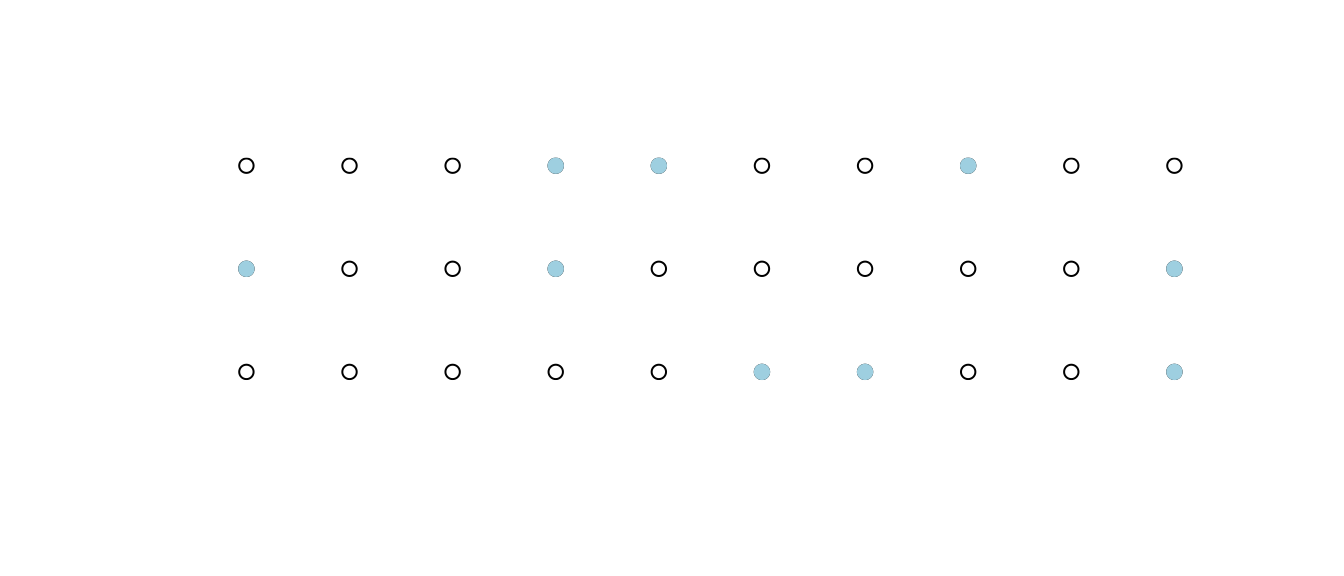
\includegraphics[width=0.9\linewidth,]{carpedatum_files/figure-latex/thirty-worlds-1} 

}

\caption{Rain (filled, blue dots) in 9 out of 30 possible worlds. It does not rain (hollow circles) in the other worlds.}\label{fig:thirty-worlds}
\end{figure}

Using this ensemble of possible worlds provides us with a sense-making device for probabilistic statements. Ultimately, it either will or will not rain tomorrow. You can also think of this observation as sampling from the ensemble of possible worlds. As though we put them all of these worlds into a hat and drew one of them. The probability of an event is thus thought of as the frequency with which it occurs.

\hypertarget{degree-of-belief}{%
\subsection*{Degree of belief}\label{degree-of-belief}}
\addcontentsline{toc}{subsection}{Degree of belief}

There is another way to think about 30\% as a probability. Suppose a meteorologist said to you, I'm 30\% sure it is going to rain tomorrow. And you say back, ``Oh, you mean that, say there are really 1000 alternate universes out there, that in roughly 300 of them, it will rain tomorrow?'' And the meteorologist says, ``I have no idea what you're talking about. There is only one universe, and I'm not totally sure what will happen tomorrow, but I put the chances of rain at 30\% \emph{{[}walks away slowly towards the door{]}}.''

For your meteorologist friend, let's call them Mel, 30\% may represent a \emph{degree of belief}. Importantly, the degree of belief is subjective. Here it is attributed to a meteorologist, which might make you take it more seriously than if your Uncle Bob said the same thing (unless Uncle Bob is actually a meteorologist). Anyway, degree of belief is subjective. Which doesn't mean it is arbitrary or just a matter of opinion. When it comes to forecasts, some people or some forecasting models are going to be right more often than others.

This idea of ``being right more often'' helps us connect the degree of belief way of thinking about probability to the ensemble sampling idea of probability. Sure, tomorrow only one universe will be ours to observe. It will either rain or not. If it rains, will you say that Mel the meteorologist did a good job or a bad job? What if it doesn't rain? It's going to be hard to say based on a single observation!

But a few days or weeks from now, Mel (the meteorologist) will come along again and say there is a 30\% chance of rain tomorrow. And again. And again some time later. What we could do is collect all of the times that Mel gave 30\% as their chance of rain and compare the actual occurrence of rain the next day. Suppose that we have 88 such cases to examine, and that it rained in 30 of them. Thats 30/88 or 34\% of the time. While not exactly 30\%, that still seems pretty good for something as complex as the weather!

\begin{quote}
Now maybe, maaaaybe, we could wonder if Mel is in fact under-predicting the chance of rain. Then we could add a bit to their forecasts when deciding what to do about it. I would feel more confident about that if we had a larger sample size. This is because we know that the observed proportions in a stochastic process will only converge to ``true'' proportions when sample sizes get large. We will come back to this in the module about money.
\end{quote}

To recap, out of 88 times that Mel gave a 30\% chance of rain tomorrow, it rained the next day 30 times and didn't rain the next day 58 times. You can see why it's hard to judge the meteorologist based on a single observation, even though we are often personally annoyed when the event (rain/no-rain) does not coincide with the choice we made about whether to wear galoshes.

\hypertarget{decisions}{%
\subsection*{Decisions}\label{decisions}}
\addcontentsline{toc}{subsection}{Decisions}

Aside from subjectivity, which is a thorny topic among statisticians, there is really no \emph{practical} difference between the interpretation of 30\% probability as a frequency of occurrence in an ensemble of possible worlds or as a degree of belief about this world. It won't change what you do about it.

If you take this forecast of rain seriously, you have decisions to make. It could be whether or not to take an umbrella with you when you leave the house tomorrow, or whether to cancel your plans to have a barbecue outside. These decisions may not seem very high stakes. The worst case scenario is that you (and others at your barbecue) get wet. But other decisions you have to make on a daily basis can have more serious consequences for your health or even your life. You often have to make those decisions based on probabilistic and maybe subjective information.

\hypertarget{death}{%
\section*{Death}\label{death}}
\addcontentsline{toc}{section}{Death}

End of warm-up. It's time to talk about when you will die.

I highly recommend this data visualization called \href{https://flowingdata.com/2015/09/23/years-you-have-left-to-live-probably/}{Years You Have Left to Live, Probably}. Here is a screenshot, although it's not nearly as interesting when you can't interact with the simulation and watch the little balls drop.

\begin{figure}[H]

{\centering 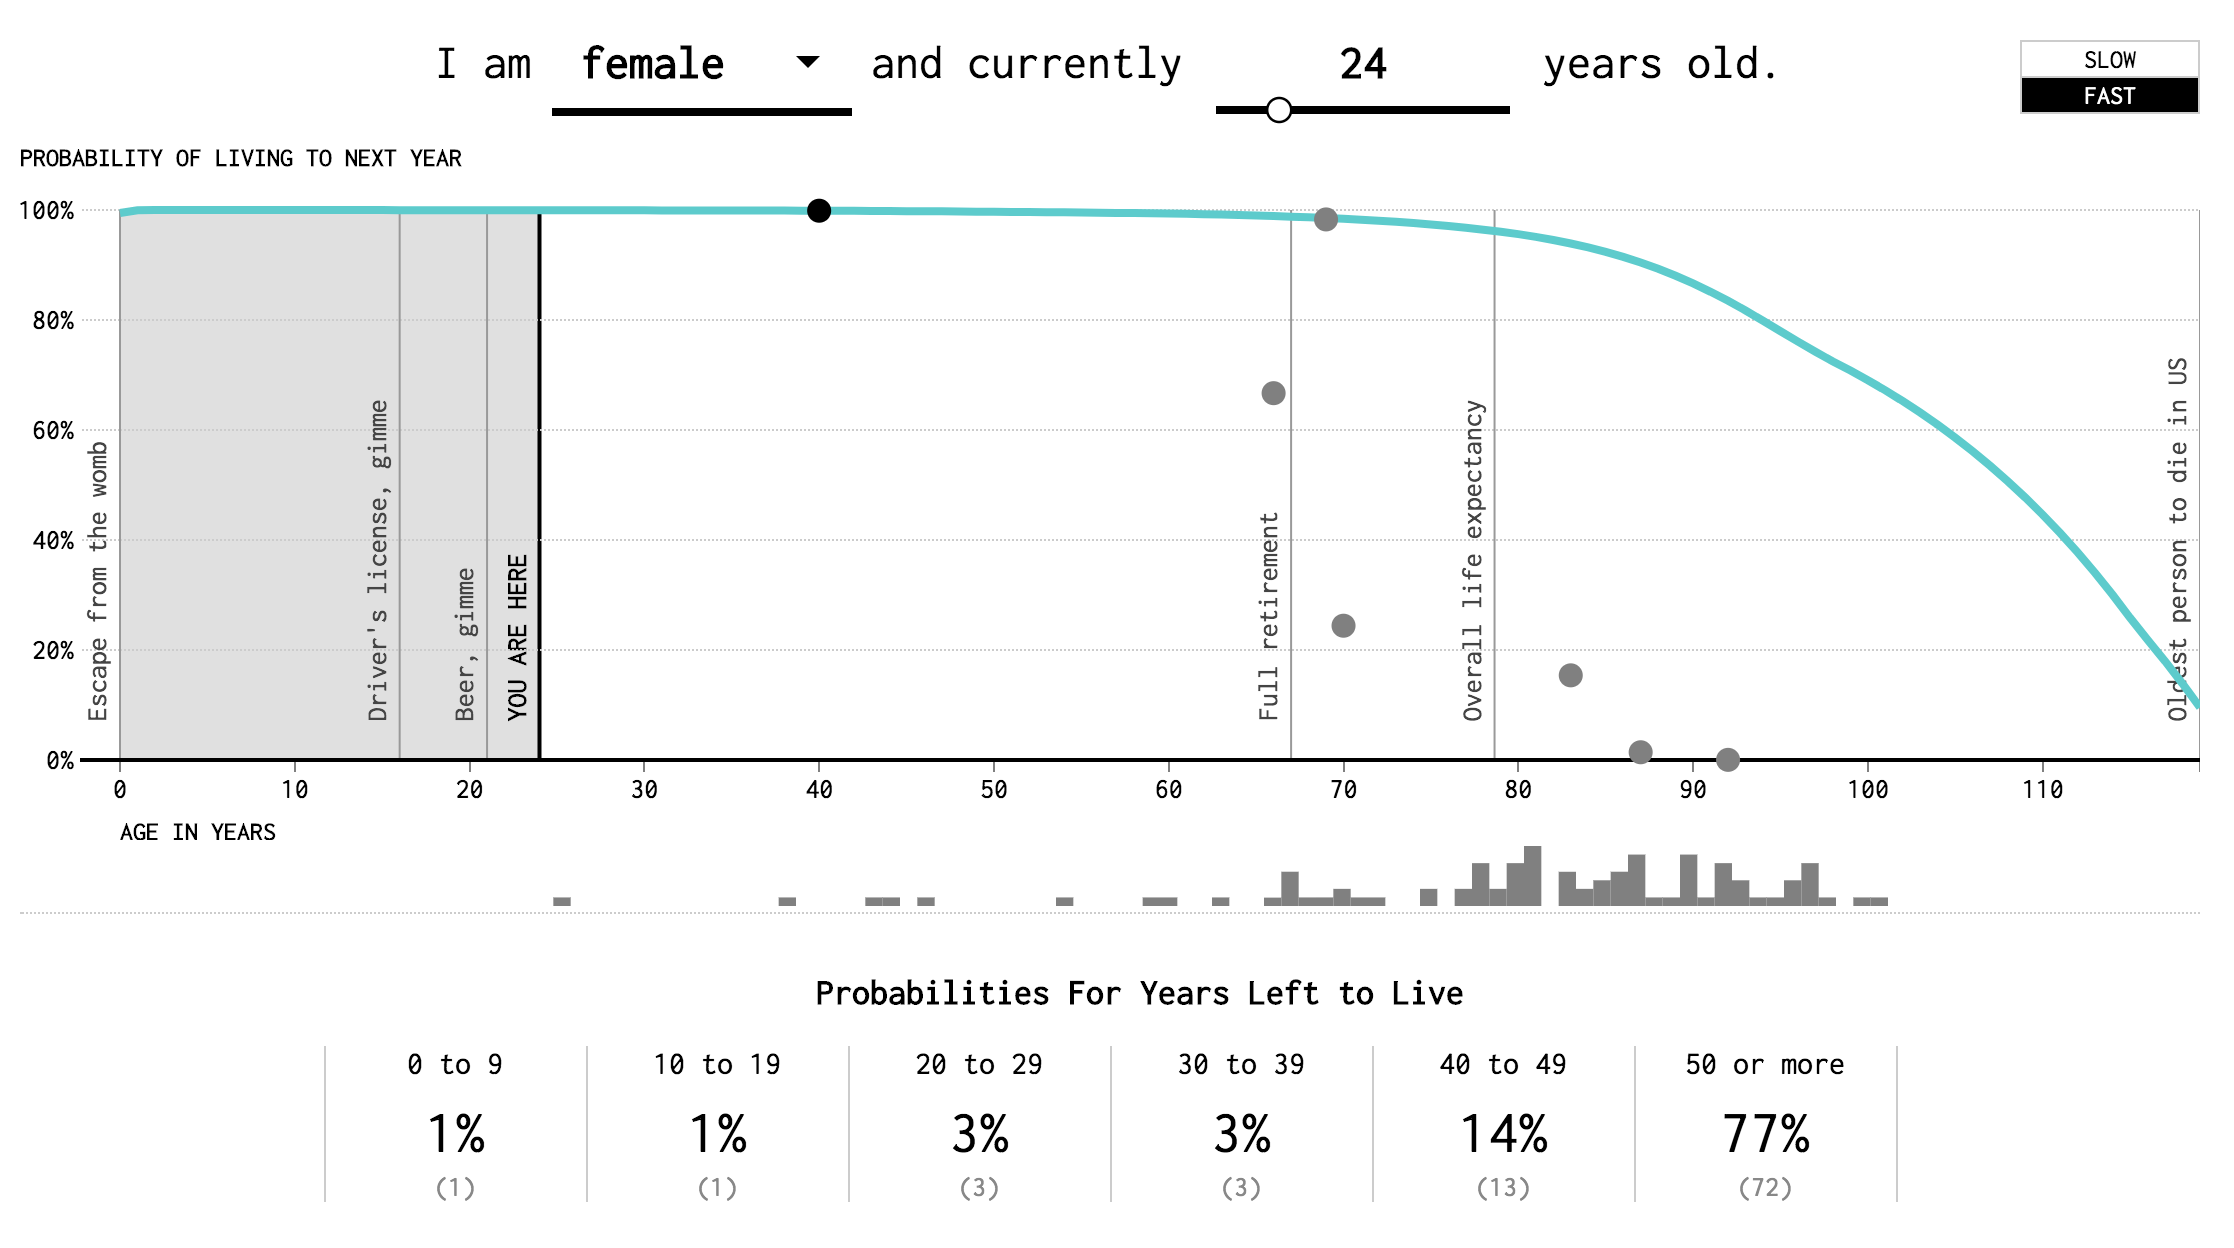
\includegraphics[width=0.9\linewidth,]{images/YYHLTLScreenshot1} 

}

\caption{Screenshot of interactive data visualization}\label{fig:years-screen}
\end{figure}

This visualization does a number of things. The most salient feature is probably the dropping balls. Each one represents a possible future outcome. This is exactly like an ensemble of alternate universes. As you watch the balls drop, you think to yourself, ``ah, nice, I lived to be 92'' and then moments later, ``ooh, harsh! I died at 39!''

As the simulation runs, it also accumulates data in bins at the bottom, labeled ``0 to 9'', ``10 to 19'', and so on. (Recall the discussion of bins, frequency tables, and histograms in Chapter \ref{shades}.) Note that these bins represent ranges of years-you-have-left-to-live, not age-at-death. This may be confusing, because age-at-death is what is shown along the horizonatal, or x-axis, of the figure. Also, right below the x-axis, and corresponding to age-at-death is a set of gray bars that grow as the balls drop. In the screenshot, the simulation has been running for a little while, so that the following counts have been accumulated.

\begin{table}[!h]
\centering
\begin{tabular}{lr}
\toprule
bin & counts\\
\midrule
0 to 9 & 1\\
10 to 19 & 1\\
20 to 29 & 3\\
30 to 39 & 3\\
40 to 49 & 13\\
\addlinespace
50 or more & 72\\
\bottomrule
\end{tabular}
\end{table}

Notice that by the time this screenshot was taken, 93 balls had dropped. The visualization took the counts, converted them into proportions of total counts (e.g., 72/93 = 0.774; 3/93 = 0.33), and represented each of these proportions as a probability, expressed as a percent (e.g., 77\%; 3\%).

Another thing that you will notice if you play around a bit is that as the balls drop, the probabilities change. In the beginning, when the number of samples (balls dropped) is small, the numbers change rapidly and sometimes by a large amount. However, after a couple of hundred samples, the changes are much smaller.

By watching the balls drop on this simulation (which I, for one, find mesmerizing), you may actually be meditating on some profound ideas in statistics. Every time you restart the simulation, you begin the sampling process. Each sample is a \textbf{draw} from some distribution of possible life outcomes. Your future life bounces around in this distribution from sample to sample. And in the beginning, when you have only collected a small number of samples, the distribution itself seems unstable. For example, if you put in 24 as the current age and start the simulation in slow mode, the estimated probability of living 40-49 more years fluctuates a lot. However, as you accumulate samples, the shape of the distribution literally comes into view as a pattern among the gray bars just below the x-axis. As the sample size increases, the probabilities becomes more stable. Eventually, if you let it run long enough, you end up with the same values, regardless of how things started out. (This increasing stability at large samples is why I was hesitant to judge Mel the meteorologist until I had more data.)

Although we are now talking about probabilities about your remaining years left to live, the interpretation of probabilities is similar to that in our discussion of rain predictions. In the case of rain, there were only two possibilities, rain or no-rain. (A dichotomy!) In the death simulation, there are six bins, each of which represents a range of years. In the case of rain, we understood the meaning of a 30\% chance (i.e., probability) of rain by imagining a large number of possible worlds, where it rains in 30\% of them. Or one universe where there are a lot of opportunities to make forecasts and check the restults of them. Thus the probability was associated directly with a frequency of something occurring. This is known is as the \textbf{frequentist} interpretation of probability. In the case of death, we say you have a 77\% chance of living 50+ more years if, in a large number of possible worlds, you live 50+ more years in 77\% of them.

You probably realize that we don't get to see all of these alternate universes, even though we can imagine them. Therefore our probability estimates in many cases are based on things that we have observed happen to \emph{other} people. For example, among 100,000 people that we do observe from the moment of birth, suppose 78\% of them lived into or past their 70s. We convert that observed frequency into a probability for you. You could say that we treat the other people we observed as alternate-universe versions of you.

\hypertarget{conditional-death}{%
\chapter{Conditional Death}\label{conditional-death}}

\hypertarget{how-does-the-death-simulation-work}{%
\subsection*{How does the death (simulation) work?}\label{how-does-the-death-simulation-work}}
\addcontentsline{toc}{subsection}{How does the death (simulation) work?}

The Flowing Data animated visualization is based on data collected in ``life tables'', which can be found online from sources like the National Center for Health Statistics (NCHS) and the Social Security Administration (SSA). Different life tables are produced every year, as life expectancy continues to evolve along with changes in health science and nutrition. Figure \ref{fig:life-duration} plots data for age-at-death (for Americans) as of 2010. There is a bar for each age from 0 to 120, and the height of each bar represents a count of deaths at that age per 100,000 people.

\begin{figure}[H]

{\centering 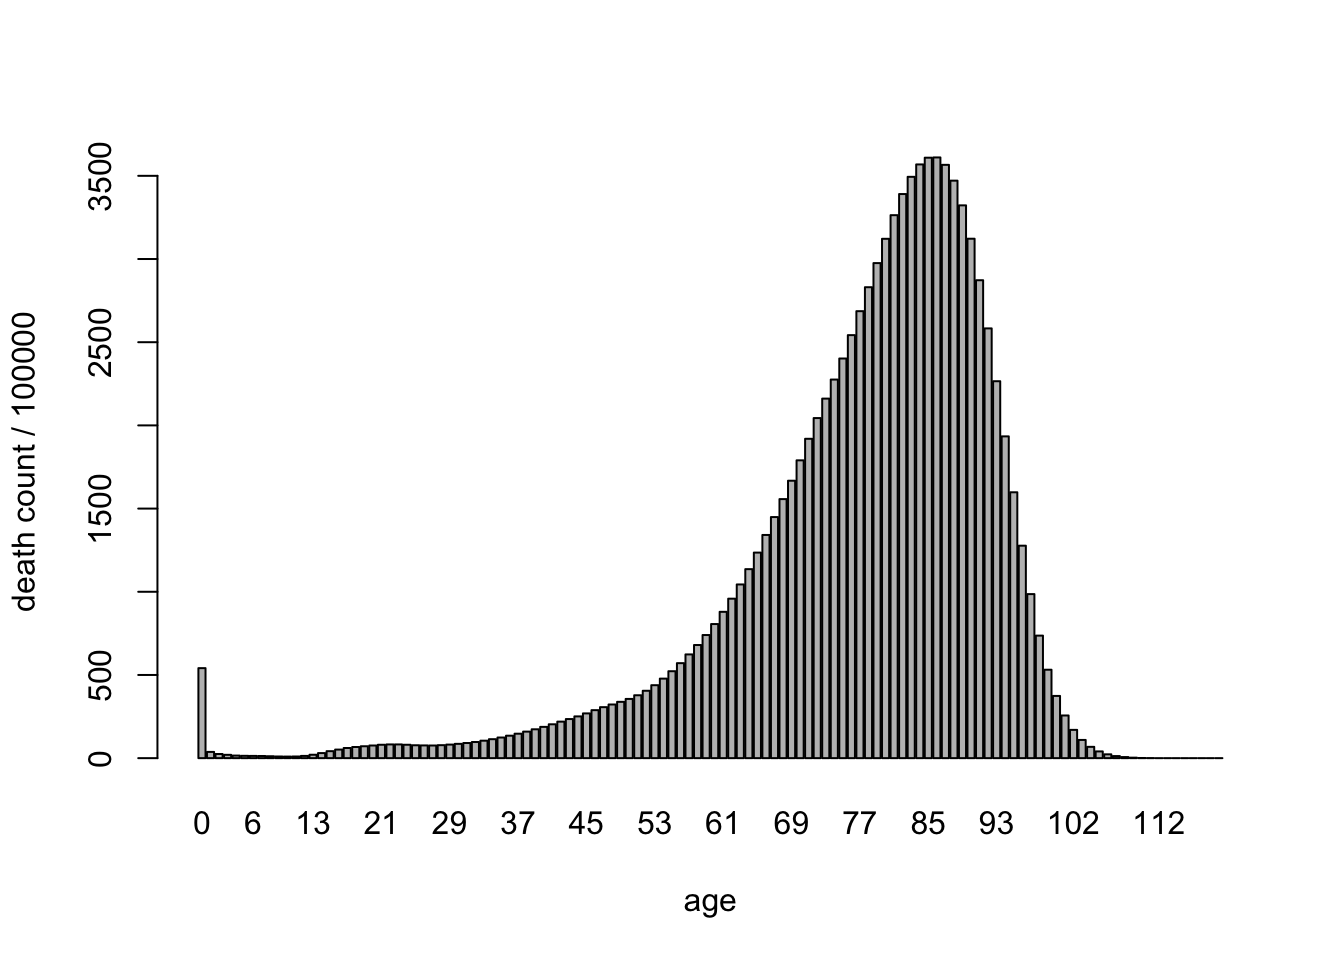
\includegraphics[width=0.9\linewidth,]{carpedatum_files/figure-latex/life-duration-1} 

}

\caption{How long Americans were living in 2010}\label{fig:life-duration}
\end{figure}

If you're like me, the first thing you notice in Figure \ref{fig:life-duration} is that little spike at age 0, like a rattle sticking up at the end of a rattle snake's tail. It shows us that roughly 5 out of 1000 babies don't make it to their first birthday. After that, your odds get considerably better for a while.

Another feature that you may detect is that the distribution of age-at-death is not symmetric. It has a long tail to the left. Distributions like this are also called left-skewed.

So how does age-at-death relate exactly to the years you have left to live? Life tables are a bit of a strange thing. First of all, they are not tables of ``raw data'' for a sample of 100,000 people. Rather, they represent a summary of data from many more deaths. According to the SSA \href{https://www.ssa.gov/OACT/HistEst/PerLifeTables/LifeTableDefinitions.pdf}{source}, ``the life table represents a hypothetical cohort of 100,000 persons born at the same instant who experience the rate of mortality represented by qx, the probability that a person age x will die within one year, for each age x throughout their lives.''

Most of us don't think about our lives in terms of questions like, are we going to die this year? But that is technically how the life table works. The life table is a set of numbers---including deaths-at-age-x and expected-years-left-to-live-at-age-x---that are all derived from one initial set of numbers which represent \emph{the probability that a person age x will die within one year}. If you're curious what that initial set of numbers looks like, I've plotted them in Figure \ref{fig:die-this-year}.

\begin{figure}[H]

{\centering 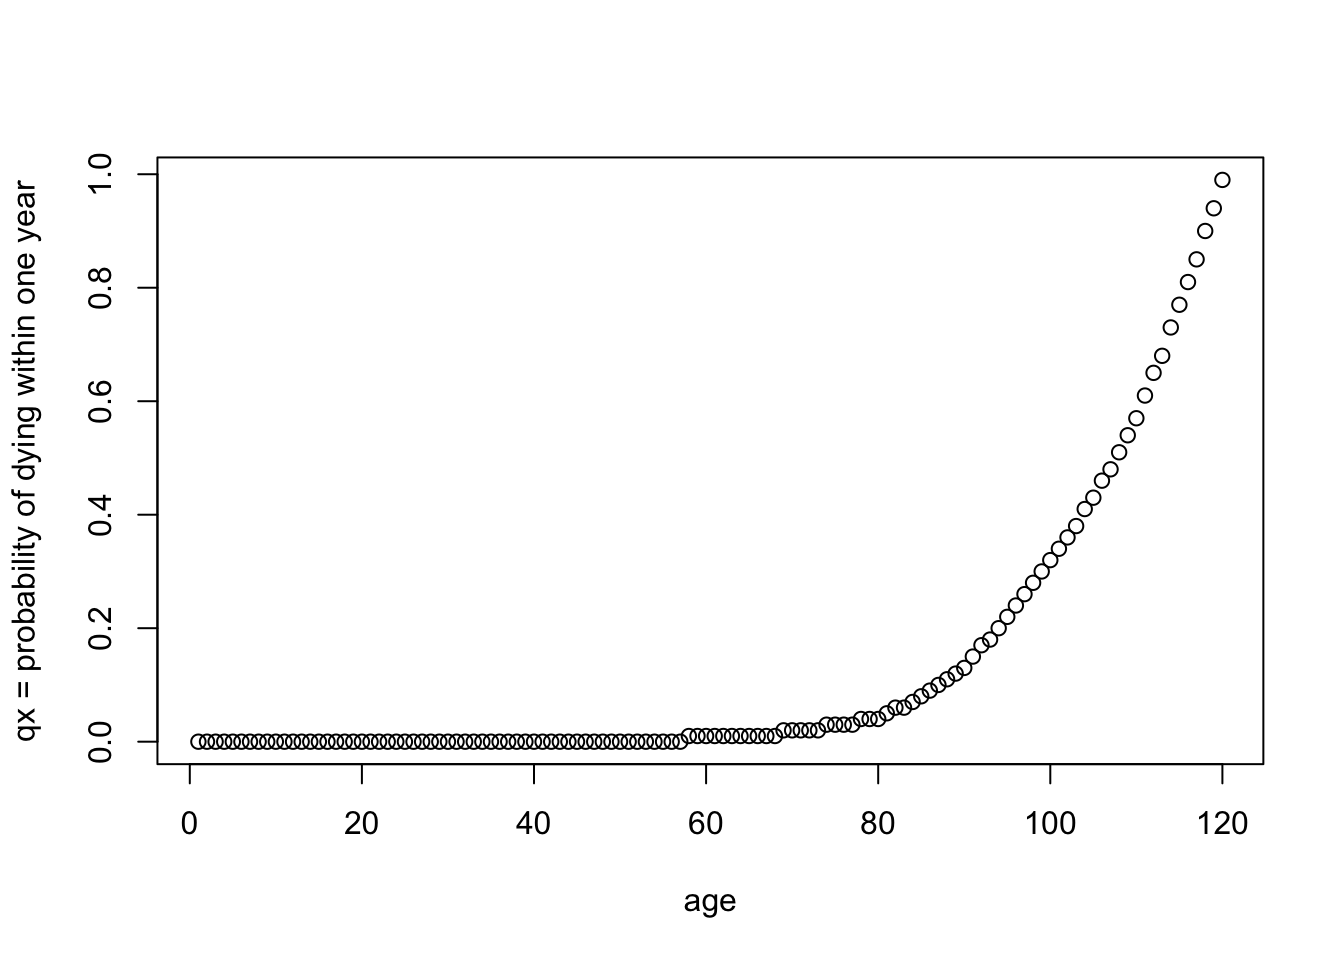
\includegraphics[width=0.9\linewidth,]{carpedatum_files/figure-latex/die-this-year-1} 

}

\caption{Mortality rate per year of age}\label{fig:die-this-year}
\end{figure}

Looking at Figure \ref{fig:die-this-year}, you can say that the probability of dying within one year gets higher as you grow older, which comes as a surprise to no one. If you're under 65, say, that probability doesn't even feel that high. It's less than 0.01 or 1\%. The probability that you will die \emph{this year} only passes 50\% after age 100. That's reassuring, right?

Well, don't get too optimistic. Your chances of dying every year may be small, but every year is another draw from this morbid lottery. If your chances of dying were 1 out of 2000, then in 2000 universes, you died in one of them. In the other 1999, you live on to another year, but then you have to press your luck again. This happens every year, and the chances slowly get worse.

But what if you wanted to know your chances, at birth, of dying in your 60s, that is between 60-69. For now, we will try to answer this question using only the life table and assuming that we know nothing else about you. The rows of the life table corresponding to this age range are these

\begin{table}[!h]

\caption{\label{tab:survival}Life Table}
\centering
\begin{tabular}[t]{lrrrrrr}
\toprule
Age & qx & lx & dx & L & Tx & ex\\
\midrule
60-61 & 0.008732 & 88745.98 & 774.97 & 88358.50 & 2051875 & 23.1\\
61-62 & 0.009335 & 87971.02 & 821.18 & 87560.42 & 1963516 & 22.3\\
62-63 & 0.009983 & 87149.84 & 870.00 & 86714.84 & 1875956 & 21.5\\
63-64 & 0.010715 & 86279.84 & 924.46 & 85817.61 & 1789241 & 20.7\\
64-65 & 0.011568 & 85355.38 & 987.39 & 84861.68 & 1703423 & 20.0\\
\addlinespace
65-66 & 0.012586 & 84367.98 & 1061.84 & 83837.06 & 1618562 & 19.2\\
66-67 & 0.013763 & 83306.15 & 1146.57 & 82732.86 & 1534724 & 18.4\\
67-68 & 0.015057 & 82159.58 & 1237.07 & 81541.05 & 1451992 & 17.7\\
68-69 & 0.016380 & 80922.51 & 1325.52 & 80259.75 & 1370451 & 16.9\\
69-70 & 0.017756 & 79596.98 & 1413.34 & 78890.31 & 1290191 & 16.2\\
\bottomrule
\end{tabular}
\end{table}

This is a lot of numbers. Recall that each qx is the mortality rate for age x, the probability of dying within one year of age x. So should you add up the qx-values for each age in the interval 60 to 69? Maybe pause here to think about this question for a moment before reading on.

Here is a partial answer. You can die at 62 and you can die at 64, but you can't die at both ages. In that sense, it was okay to add the probabilities of these events because they are \textbf{disjoint}, i.e., they can't both happen and you are interested in whether any one of them does happen. However, if you add up these probabilities, you will still over-estimate the probability for a different reason. Can you guess what you've left out?

Here is the rest of the answer. You've left out the fact that these probabilities assume that you have already made it to 60, and there's a chance (at birth) that you won't.

To answer the original question, you want to add up the following probabilities:

\begin{verbatim}
(Probability of making it to 60 and then dying at 60) + 
(Probability of making it to 61 and then dying at 61) + 
... +
(Probability of making it to 69 and then dying at 69) + 
\end{verbatim}

How do you figure out the probability of making it to 60 without dying? It sounds a little bit like a riddle whose answer is ``one year at a time.'' Indeed, to make it to 60 without dying, you need to not die every year for the first 59 years of your life.

Note that, while death can occur in only one year of your life, to survive into your sixties you need ALL of the following to be true: NOT dying at 0 AND NOT dying at 1 AND \ldots{} NOT dying at 59. The probability of each event (not dying in each year) is independent, and the probability that all of them happen is the product of the individual probabilities.

\begin{verbatim}
Probability of NOT dying at 0 * 
Probability of NOT dying at 1 having made it to 1 * 
... * 
Probability of NOT dying at 59 having made it to 59
\end{verbatim}

Since in any given year, you either die or don't die, these two probabilities must add up to 1, so having gotten to any age x, the probability of surviving it is (1-qx). Now we can take the product of (that is, multiply) all of the survival probabilities (1 - qx) for each x from 0 up to age 59. (I will include the code here. The data table I have loaded from the National Center for Health Statistics is called ``lifetableNCHS'').

\begin{Shaded}
\begin{Highlighting}[]
\FunctionTok{prod}\NormalTok{(}\DecValTok{1}\SpecialCharTok{{-}}\NormalTok{lifetableNCHS[}\DecValTok{1}\SpecialCharTok{:}\DecValTok{60}\NormalTok{,}\StringTok{"qx"}\NormalTok{])}
\end{Highlighting}
\end{Shaded}

\begin{verbatim}
## [1] 0.887458
\end{verbatim}

You may notice that this probability had already been calculated for you in the life table, but it had been presented slightly differently as column lx, which is the number of persons (in a cohort of 100,000) surviving to exact age x. If we multiply our rate by 100000, we get 88745.8, which (up to a rounding error) is the same as the number in Table \ref{tab:survival}.

Okay, so now we are ready to complete the probability calculation. Recall we wanted to add up ten things: Probability of making it to 60 and then dying at 60, etc. We know that the probability of making it to age x is the same as the value of column lx in the table divided by 100,000. And the probability of dying is qx. So we need to multiply these two numbers in each row and add them up.

The result is 0.1056. An American child born in 2010 has a 10.5\% chance of dying in their 60s (and a 20.7\% chance of dying in their 70s).

So, we've figured out how to do that. And we're almost ready to move on, but it is worth noticing something. The product of the value qx and lx in each row of the life table is the value dx, which is the number of deaths at age x (or between x and x+1). So when we multiplied and added before, we were really just adding up the number of deaths (dx) at ages 60-69 and dividing by 100,000.

Now hopefully that makes sense to you that this should give us the answer we were originally looking for, namely what are the chances, at birth, of dying in your 60s. We could have looked at our hypothetical cohort of 100,000 people all born at the same time and asked: how many of them will die in their 60s. Well, that would be the sum of the dx-values, namely 10562. It wouldn't be a probability, though, unless we divided it by the total number of people (100,000).

So we've shown that we can answer our particular question two different ways:

\begin{enumerate}
\def\labelenumi{\Alph{enumi})}
\tightlist
\item
  Computing the total probability of your making it to 60 and then dying at 60 \emph{or} making it to 61 and dying at 61 \emph{or} making it to 62 and dying at 62 etc. up to age 69.
\end{enumerate}

or

\begin{enumerate}
\def\labelenumi{\Alph{enumi})}
\setcounter{enumi}{1}
\tightlist
\item
  Computing the overall proportion, out of 100,000 people, who die in their 60s.
\end{enumerate}

A = B in this case. An important property of mathematical sciences is that you can arrive at the same answer in different ways. Maybe that sounds like a waste of time, but I view it as one of the most reassuring things about math. If you try something two different ways, and you do \emph{not} get the same answer even though you should, then something is probably wrong with the way you are thinking about it.

\hypertarget{somefacts}{%
\chapter{Some facts about Probabilities}\label{somefacts}}

In this course, I have taken the strong position that ideas should be driven by questions. So I've tried to reason through the example above before setting up any foundations on the basic rules of probability. A standard introduction to these topics can be found in many books, for example OpenIntro Stats, Chapter 3.

Now is probably a good time to recap some of what we have established about probabilities. We will also introduce the most basic notation \texttt{P(A)} for the probability that event A happens. For example, event A can stand for ``you die at age 64'' or ``it rains in New York tomorrow.''

\begin{itemize}
\tightlist
\item
  When possibilities are disjoint, or mutually exclusive, the probability that either one of them happens is the sum of the individual probabilities
\end{itemize}

\begin{quote}
\begin{verbatim}
P(A or B) = P(A) + P(B)
\end{verbatim}
\end{quote}

An example of this was dying at age 62 or dying at age 64.

\begin{itemize}
\tightlist
\item
  A special case of this addition rule applies when one or the other MUST happen. For example, in logic, either something happens or it doesn't happen. Either A or NOT A. Since these possibilities are disjoint:
\end{itemize}

\begin{quote}
\begin{verbatim}
P(A) + P(not A) = 1
\end{verbatim}
\end{quote}

\begin{quote}
\begin{verbatim}
P(not A) = 1 - P(A)
\end{verbatim}
\end{quote}

An example of this was the probability that you do not die at age 0. We found it by subtracting out the probability that you will die from 1.

The last fact we used is

\begin{itemize}
\tightlist
\item
  The joint probability rule for \textbf{independent} events that BOTH occur is the product of the individual probabilities of each event occurring.
\end{itemize}

\begin{quote}
\begin{verbatim}
P(A and B) = P(A) * P(B)
\end{verbatim}
\end{quote}

We used that to figure out how you survive by not dying every year. Notice that I've snuck in the word independent (well, I snuck it in boldy, so it wasn't that sneaky). There is an intuitive reason why it is important to make a distinction about independent events.

In the last module, we said that two events (we were talking about responses to questions) are independent if knowing about one of them does not give you any information about what the other one might be. But remember bizarro world where the toilet paper orientation and peanut butter preference were deterministically related, and specifically everyone is either under-chunky or over-smooth? I've reproduced this result in Table \ref{tab:tpxpb-reprise}. If I told you that 53\% of the total population prefers smooth, then what proportion of the total population prefers smooth AND likes to over-hang? Also 53\%. What proportion prefers smooth AND under-hangs? 0!

\begin{table}[!h]

\caption{\label{tab:tpxpb-reprise}Bizarro world}
\centering
\begin{tabular}[t]{lrr}
\toprule
  & chunky & smooth\\
\midrule
over & 0 & 23\\
under & 17 & 0\\
\bottomrule
\end{tabular}
\end{table}

In bizarro world, toilet paper orientation and peanut butter preference are NOT independent, because knowing one of them DOES give you information about the other.

\begin{verbatim}
P(tp = over AND pb = smooth) does NOT equal to P(tp = over) * P(pb = smooth)
\end{verbatim}

This will become even more clear in the next section.

\hypertarget{conditional-probabilities}{%
\section*{Conditional Probabilities}\label{conditional-probabilities}}
\addcontentsline{toc}{section}{Conditional Probabilities}

Recall that we would NOT have gotten the right answer to the probability of dying in your 60s if we added up the mortality rates qx for all ages x in {[}60-69{]}. (Exercise: verify this.) Rather, we had to multiply these numbers first by the probability of living to age x. Another way to say this is that the mortality rate qx was actually a \textbf{conditional probability.} It was the probability of dying at age x \emph{on condition that} you have survived to age x. To be absolutely clear, we are measuring x in whole numbers, like birthdays, but we don't mean dying on your xth birthday. Rather, we mean dying anytime between turning age x and turning x+1. We need a special notation to distinguish conditional probabilities. We write,

\begin{verbatim}
qx = P(You die at age x | You survived to age x)
\end{verbatim}

and we read this as ``qx is the probability that you die at age x given that you survived to age x'' or as ``qx is the probability that you die at age x conditional on your surviving to age x.'' These are equivalent, but they differ from

\begin{verbatim}
P(You die at age x)
\end{verbatim}

which is the \textbf{unconditional} probability that you die at age x. This is also different from

\begin{verbatim}
P(You die at age x AND You survived to age x)
\end{verbatim}

which is called the \textbf{joint probablity} of the two events. (Note that the joint probability of events A and B is also often written as P(A, B). The comma functions like the word ``and''.) We calculated exactly this joint probability above when we wanted to add up the probabilities that you die at some point in your 60s. The way we computed the joint probability for each year was by application of this general rule for conditional probabilities

\begin{verbatim}
P(A and B) = P(A|B) P(B)
\end{verbatim}

which we read as ``the probability of both A and B happening is equal to the probability of A conditional on B multiplied by the probability of B.'' Note that this rule \emph{always} holds. That's because what I've called the general rule is equivalently just the definition of conditional probability. For example, I could have written it this way:

\begin{verbatim}
P(A|B) = P(A and B) / P(B)
\end{verbatim}

This is just a rearrangement of the formula, but we have a tendency of seeing whatever is on the left side of an equation as being defined by what is on the right.

As far as death is concerned, the following are all true:

\begin{verbatim}
P(die at x AND survived to x) = P(die at x | survived to x) * P(survived to x)
P(die at x AND survived to x) = qx * P(survived to x)

qx = P(die at x AND survived to x) / P(survived to x)
\end{verbatim}

where in the second line I substituted the mortality rate qx for the conditional probability that defines it. In the last line, you can see how the mortality rate could be estimated from data if you actually observed a whole bunch of people. You would count how many of the die at age, say, 62, and divide that number by the number who survived to age 62. You can also probably see why the following is true:

\begin{verbatim}
P(survived to x | die at x) = 1
\end{verbatim}

That is, if you died at 62 then you must have survived to that age. That may seem too obvious for words, but it helps to show clearly that for conditional probabilities, it is not generally true that P(A\textbar B) = P(B\textbar A).

Considering toilet paper in bizarro world, we can see explicitly why the rule for joint probabilities of independent events \texttt{P(A\ and\ B)\ =\ P(A)\ *\ P(B)} did not hold. The conditional probability relationship always holds, but independence is a special case. We can see what it is now:

\begin{verbatim}
P(A and B) = P(A|B) P(B) = {only in special cases} = P(A) * P(B)
\end{verbatim}

Thus, when A and B are independent, it must be true that

\begin{verbatim}
P(A|B) = P(A)   # for independent events
\end{verbatim}

which reads as ``the probability of A conditional on B is equal to the probability of A (regardless of B).'' Another way to say this is that no matter what we know about B, it doesn't tell us anything informative about A.

In the real world, this is true about toilet paper and peanut butter.

\begin{verbatim}
P(tp = over | pb = smooth) = P(tp = over) ## real world
\end{verbatim}

But that was NOT true in bizarro world, where knowing peanut butter preference told us EVERYTHING about toilet paper orientation. If A is the probability that a person is an over-hanger, and B is the probability that they prefer smooth peanut butter, then

\begin{verbatim}
P(tp = over | pb = smooth) = 1  ## bizarro world
P(tp = over | pb = chunky) = 0
\end{verbatim}

However, regardless of whether we stay in the real world or in bizarro world, the following will always be true,

\begin{verbatim}
P(tp = over AND pb = smooth) =  P(tp = over | pb = smooth) * P(pb = smooth),
\end{verbatim}

because this is the definition of conditional probability. Now you might notice that if the above is true, then the following should \emph{also} be true:

\begin{verbatim}
P(pb = smooth AND tp = over) =  P(pb = smooth | tp = over) * P(tp = over).
\end{verbatim}

And it is true. For the same reason that this follows from the definition of conditional probability.

The order of the two joint events on the left-hand-side does not matter. There is no difference between P(A and B) and P(B and A). If both A and B happen, they both happen. There is no implied chronology when we write ``A and B'' that A came before B. So, that said, it is also true that

\begin{verbatim}
P(tp = over | pb = smooth) * P(pb = smooth) =  P(pb = smooth | tp = over) * P(tp = over).
\end{verbatim}

By combining the two equations from above. Or, in general

\begin{verbatim}
P(A | B) * P(B) =  P(B | A) * P(A)
\end{verbatim}

Notice that is \emph{not} generally true about conditional probabilities that \texttt{P(A\textbar{}B)\ =\ P(B\textbar{}A)}. Even though it is always true about joint probabilities that \texttt{P(A,B)\ =\ P(B,A)} (I used commas instead of ``and'' here.) Here's an example. All NYU students are New Yorkers (at least, honorary New Yorkers while in town.) But not all New Yorkers are NYU students. The probability of being a New Yorker conditional on (or given that) you are currently an NYU student is 1. However the probability of being an NYU student conditional on being a New Yorker is clearly not 1.

\hypertarget{conditional-death-again}{%
\section*{Conditional death, again}\label{conditional-death-again}}
\addcontentsline{toc}{section}{Conditional death, again}

Earlier I said we would use the life table to answer questions about when you will die assuming nothing else about you. Now, you might be aware that life expectancy is not the same for males and females. Indeed, there are separate life tables for each sex. I've plotted the death column dx from both tables in Figure \ref{fig:life-durationMF}. Females are shown in light blue bars, and males using orange. Unfortunately for the males, their mortality rate is higher not only in their later years, but even in their late teens and twenties. (We'll come back to that when we consider how you will die.)

\begin{figure}[H]

{\centering 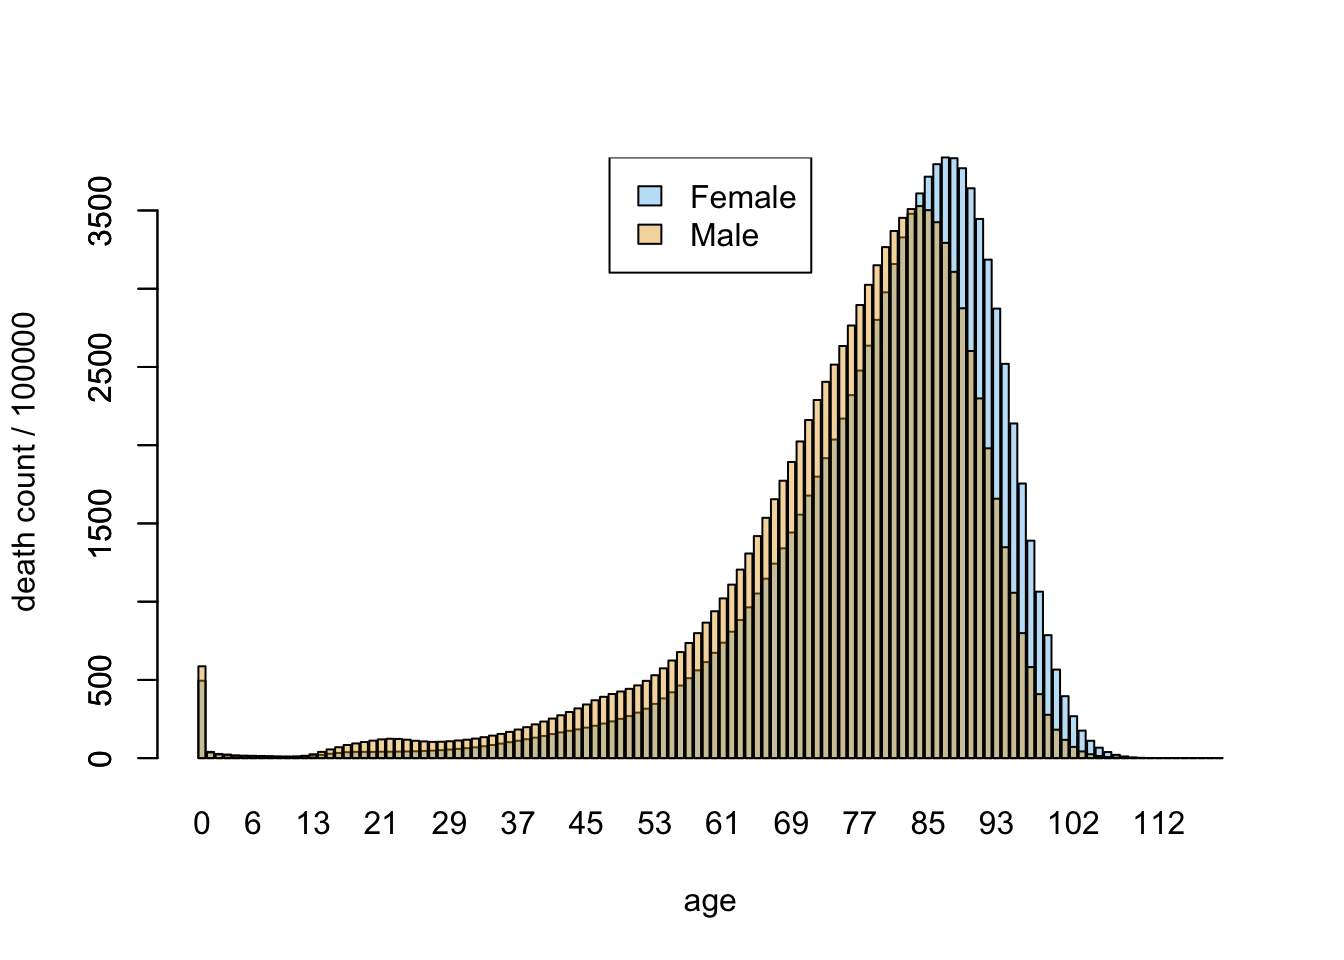
\includegraphics[width=0.9\linewidth,]{carpedatum_files/figure-latex/life-durationMF-1} 

}

\caption{Deaths by age for male and female (2010)}\label{fig:life-durationMF}
\end{figure}

Suppose I was interested purely in the likelihood (at birth) of living into ones 90s or beyond, conditional on sex. I can find out the proportions from separate life tables for each sex as follows. (These single-sex life tables go from 0 to 119, and the first row is dying before your 1st birthday. I need to look at the 91st row to see death after age 90.):

\begin{Shaded}
\begin{Highlighting}[]
\CommentTok{\#proportion of females dying from at ages 80{-}119}
\FunctionTok{sum}\NormalTok{(lifetableFemale[}\DecValTok{91}\SpecialCharTok{:}\DecValTok{120}\NormalTok{,}\StringTok{"dx"}\NormalTok{])}\SpecialCharTok{/}\FunctionTok{sum}\NormalTok{(lifetableFemale[,}\StringTok{"dx"}\NormalTok{])}
\end{Highlighting}
\end{Shaded}

\begin{verbatim}
## [1] 0.2446278
\end{verbatim}

\begin{Shaded}
\begin{Highlighting}[]
\CommentTok{\#proportion of males dying from at ages 80{-}119}
\FunctionTok{sum}\NormalTok{(lifetableMale[}\DecValTok{91}\SpecialCharTok{:}\DecValTok{120}\NormalTok{,}\StringTok{"dx"}\NormalTok{])}\SpecialCharTok{/}\FunctionTok{sum}\NormalTok{(lifetableMale[,}\StringTok{"dx"}\NormalTok{])}
\end{Highlighting}
\end{Shaded}

\begin{verbatim}
## [1] 0.1347719
\end{verbatim}

I can make a two way table using these proportions. I will base my table on a sample of 1000 females and 1000 males. \textbf{This is not real sample data.} I am just using the life table proportions here to construct an idealized sample.

\begin{Shaded}
\begin{Highlighting}[]
\NormalTok{sex\_age80 }\OtherTok{\textless{}{-}} \FunctionTok{data.frame}\NormalTok{(}\AttributeTok{dieBefore90 =} \FunctionTok{c}\NormalTok{(}\DecValTok{755}\NormalTok{,}\DecValTok{865}\NormalTok{), }\AttributeTok{livePast90 =} \FunctionTok{c}\NormalTok{(}\DecValTok{245}\NormalTok{,}\DecValTok{135}\NormalTok{), }
                        \AttributeTok{row.names=}\FunctionTok{c}\NormalTok{(}\StringTok{"Females"}\NormalTok{,}\StringTok{"Males"}\NormalTok{))}
\end{Highlighting}
\end{Shaded}

The table looks like this

\begin{table}[!h]

\caption{\label{tab:unnamed-chunk-19}Will you live into your 90s?}
\centering
\begin{tabular}[t]{lrr}
\toprule
  & dieBefore90 & livePast90\\
\midrule
Females & 755 & 245\\
Males & 865 & 135\\
\bottomrule
\end{tabular}
\end{table}

The unconditional probability of living past 90 is (245+135)/2000 = 0.19 or 19\%. This would be your betting chances if a baby were born and you did not know its sex. We can write this as P(live past 90) = 0.19. But if you knew it was born female, then you need to compute P(live past 90 \textbar{} sex = female). How would you do this? Well, you can use the table. Of the 1000 females, 245 live past 90, so the answer is 24.5\%. For males, it is 13.5\%. Sorry, males.

\hypertarget{just-to-make-things-weird}{%
\subsection*{Just to make things weird}\label{just-to-make-things-weird}}
\addcontentsline{toc}{subsection}{Just to make things weird}

Now suppose, for arguments' sake, that the numbers in the life table apply to everyone born in the last 120 years as of today (they don't; life expectancy has changed over the years). If I told you that someone was over 90, but nothing else about them, what is the probability that the person was female at birth (we will make the simplifying assumption that the life table corresponds to sex at birth)? The two-way table I constructed had equal numbers of males and females. We will assume that the birth rates are indeed the same. So the unconditional probability of being born female knowing nothing about a person's status as living or dead is 50\%. However, among those alive in their 90s, 245/(245+135) = 0.64 of them are female. Almost 2 to 1.

Given a two-way table, with variables representing events A and B, it is possible to derive conditional probabilities in both directions. P(A\textbar B) might be the probability of living past 90 given sex at birth. P(B\textbar A) would then be probability of sex at birth given present age over 90.

In the next chapters, we will start to examine what kinds of things might kill you. This will give us another chance to look at association in two way tables (as distinguished from independence). We will also explore what it means to say that something \emph{causes} early death. In the example above, we saw that sex is associated with early death. Females live longer; males die younger. Would we say that sex causes early death?

\hypertarget{how-you-will-die-causes-or-conditions}{%
\chapter{How You Will Die: Causes or Conditions?}\label{how-you-will-die-causes-or-conditions}}

\hypertarget{causes-of-death-colloquially}{%
\section*{Causes of death, colloquially}\label{causes-of-death-colloquially}}
\addcontentsline{toc}{section}{Causes of death, colloquially}

We now pause our inquiry into when you will die and concentrate for some time on how it might happen. Let us pay another visit to Nathan Yau's series of (interactive) visualizations for Flowing Data. We already discussed \href{https://flowingdata.com/2015/09/23/years-you-have-left-to-live-probably/}{Years You Have Left to Live, Probably}. Another of them is called \href{https://flowingdata.com/2016/01/05/causes-of-death/}{Causes of Death} and the last \href{https://flowingdata.com/2016/01/19/how-you-will-die/}{How you will die} (links work if you download the PDF but do not work within Perusall).

These visualizations are really a treasure trove. So much going on. I've reproduced an image from Causes of Death below, but you really should interact with it on the web.

\begin{figure}

{\centering 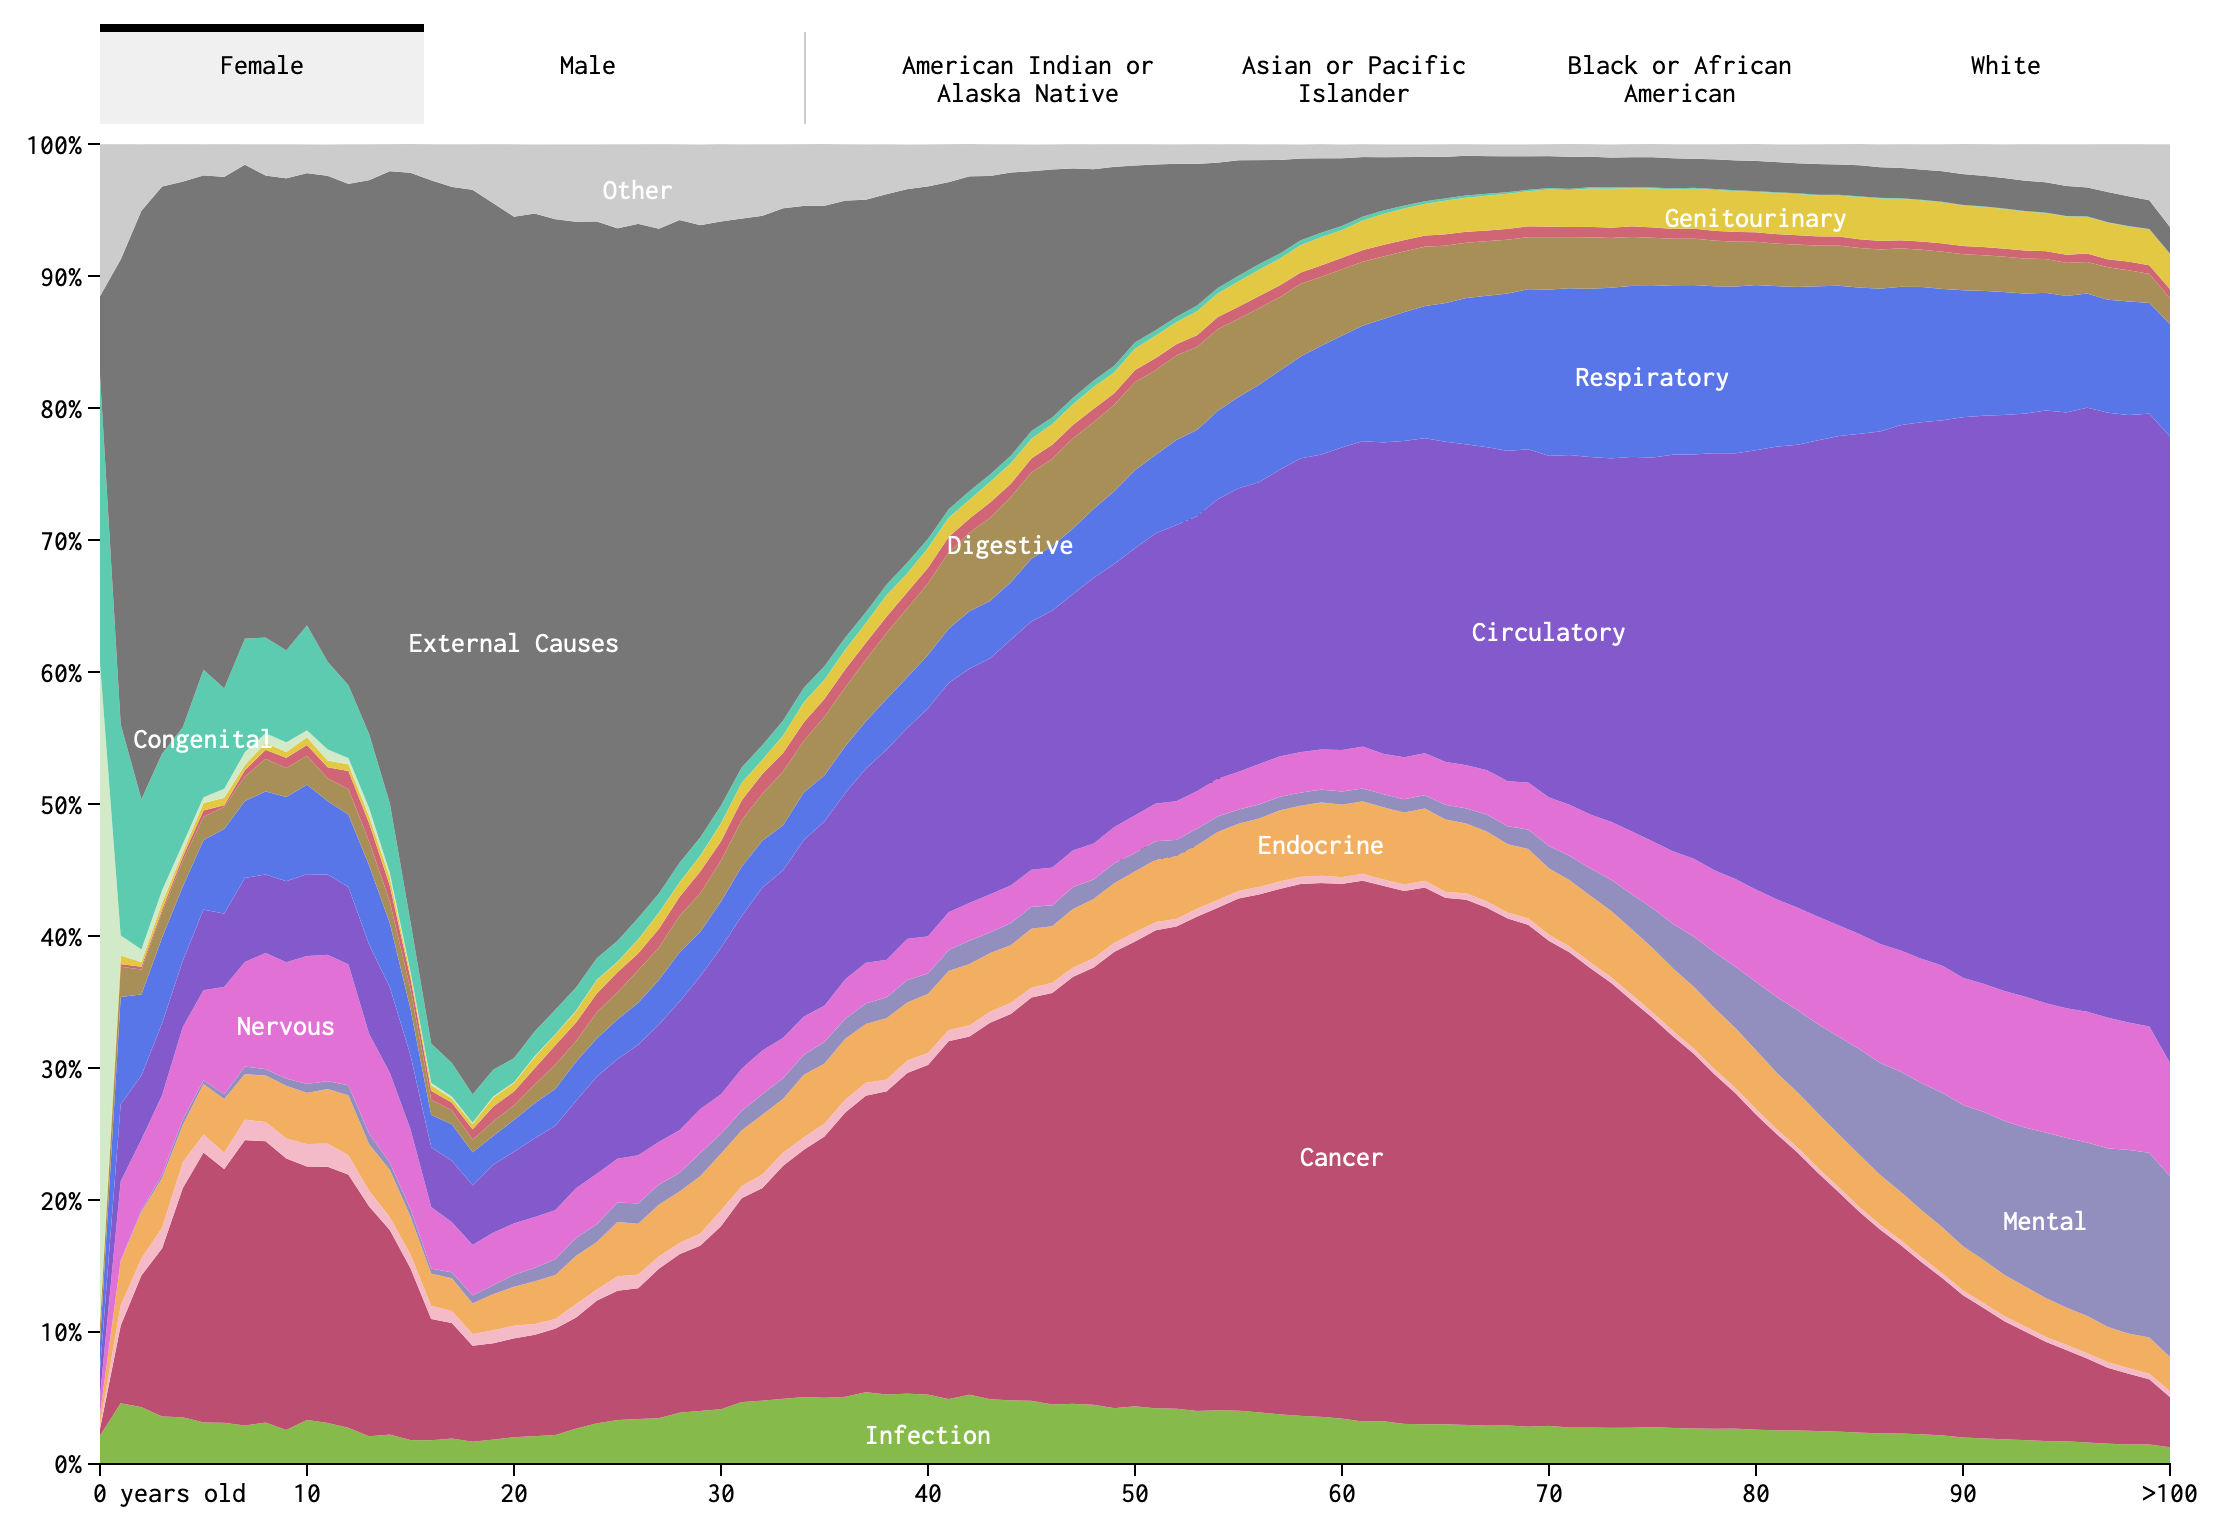
\includegraphics[width=0.9\linewidth]{images/CausesOfDeath} 

}

\caption{Screenshot of Causes of Death visualization}\label{fig:causes-viz}
\end{figure}

Take a close look at the image in Figure \ref{fig:causes-viz}. How many variables are represented here? (Pause and think this over.) There are fifteen color bands representing causes of death, but these are not each variables. Rather, they are categories of a single variable: cause-of-death, as operationalized by the Centers for Disease Control and Prevention.\footnote{Operationalization of a variable is a fancy and more specific word for defining it. It doesn't seem necessary to define ``cause of death'' in the common-sense use of the word define. But when we decide how many and which categories to include in our use of the variable, we operationalize this definition. For example, we could operationalize cause of death as ``natural causes'' or ``other''. This would be a dichotomous operationalization. And it leaves a lot to the imagination. The Center for Disease Control is particularly interested in diseases and not in external causes. So it makes sense that all external causes are banded together in this figure. However, don't be fooled. There are many subcategories, including very specific ones like ``Pedal cyclist injured in collision with heavy transport vehicle or bus.''} These include cancer, congenital defects, and external causes (e.g., pianos falling on your head), among others. Along the bottom of the image we see age, which is another variable. Indeed, the most salient aspect of this visualization is how much the relative importance of different causes of death changes over the course of one's life span.

If you die in your 20s, it is likely that you died from external causes. While if you died in your 80s, it is more likely because of a circulatory or respiratory disease. This intuitive sense-making is an example of conditional probabilities. It may not be a two-way table, but Figure \ref{fig:causes-viz} is in many ways analogous to a two-way table. The two variables are age-at-death and cause-of-death. Although we are not putting numbers to the probabilities we can read this image as indicating that

\begin{verbatim}
P(cause = external | age in 20s) > P(cause = circ or resp | age in 20s)
\end{verbatim}

(read, the probability that cause of death is external \emph{given} that age of death is in ones 20s\ldots).
While the opposite is true in your 80s:

\begin{verbatim}
P(cause = external | age in 80s) < P(cause = circ or resp | age in 80s)
\end{verbatim}

There is an important difference between this particular figure and a two-way table of counts. This figure shows \emph{relative} proportions of death for each age, not absolute numbers. As we know, and even visualized explicitly in Chapter \ref{conditional-death}, the count of deaths is much higher among adults in their 70s and 80s than among those in their 20s. Figure \ref{fig:causes-viz} does not communicate that. Instead, by ignoring the overall scale, the figure allows us to focus on the shifting importance of different causes.

A two dimensional figure is used here to represent relationships between two variables (age-at-death and cause-of-death), but there are more than two variables here. The additional variables require using the tabs at the top. Sex is here, as well as race. Note that although sex and race categories are all switched between by using tabs, they are not, of course, categories belonging to a single variable. This is something that I slightly dislike about this visualization. The way it is designed, it feels as though one cannot observe, or condition on, sex and race at the same time.

So there are four variables (did you get it right?). We can, in principle, imagine conditioning on any or all of them. For example, we could ask what is the probability of death by endocrine disease for (i.e., given, conditioned on) an African-American male aged 65-70. We might write something like this in probability notation as,

\begin{verbatim}
P(cause = endocrine | race = African-American, sex= male, age = 65-70) = ?
\end{verbatim}

Yau also draws your attention to another feature of this visualization: ``When you select races, you might notice that the smaller groups, American Indian and Asian, appear to be more jagged, whereas cause of death for the larger groups, black and white, appear to be smoother. This is likely due to population size more than anything else. It's a smaller sample, and there's higher variance.''

The sample size factors in here, because CDC data are being used to estimate a proportion. For example, what proportion of 65-year-old deaths are the result of circulatory disease. Suppose we knew the true proportion in the total population. If we took only a sample from this population, we will not always find exactly the same proportion. For small samples, the proportion in each sample will appear to vary a lot. While for large samples, the proportion will vary but in a smaller range. We will revisit this idea again when we discuss making bets.

Yau's final visualization in the trio, How You Will Die, combines elements of causes-of-death and years-you-have-left-to-live. The visualization is dynamic, and the passing of time is like a sped up version of your life. In Figures \ref{fig:how-die-21-1}-\ref{fig:how-die-21-3}, I have reproduced still snapshots taken at three different ``ages'', starting with the simulation settings: Asian female, age 21.

\begin{figure}

{\centering 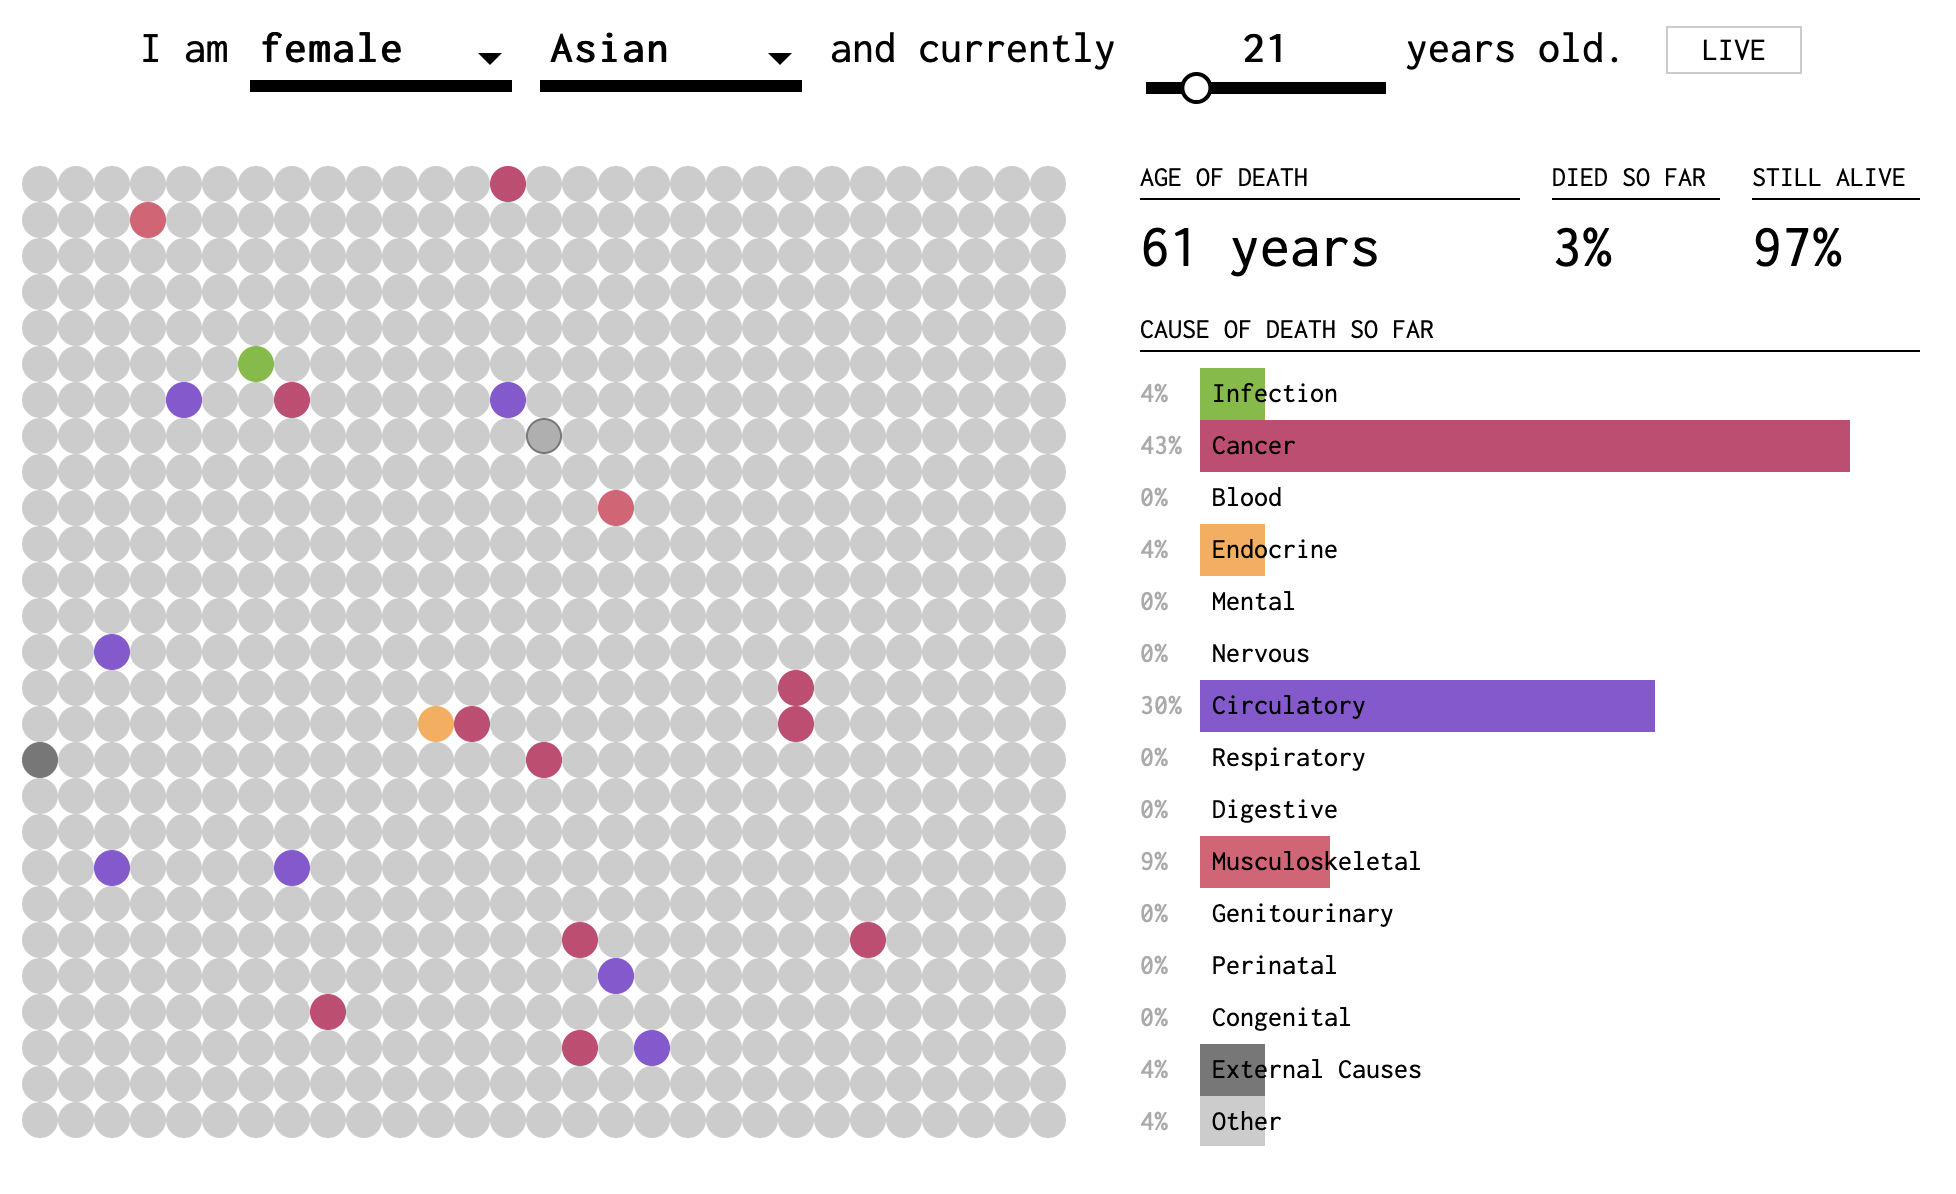
\includegraphics[width=0.8\linewidth]{images/HowYouWillDie21-61} 

}

\caption{Screenshot 1 of How You Will Die visualization}\label{fig:how-die-21-1}
\end{figure}

\begin{figure}

{\centering 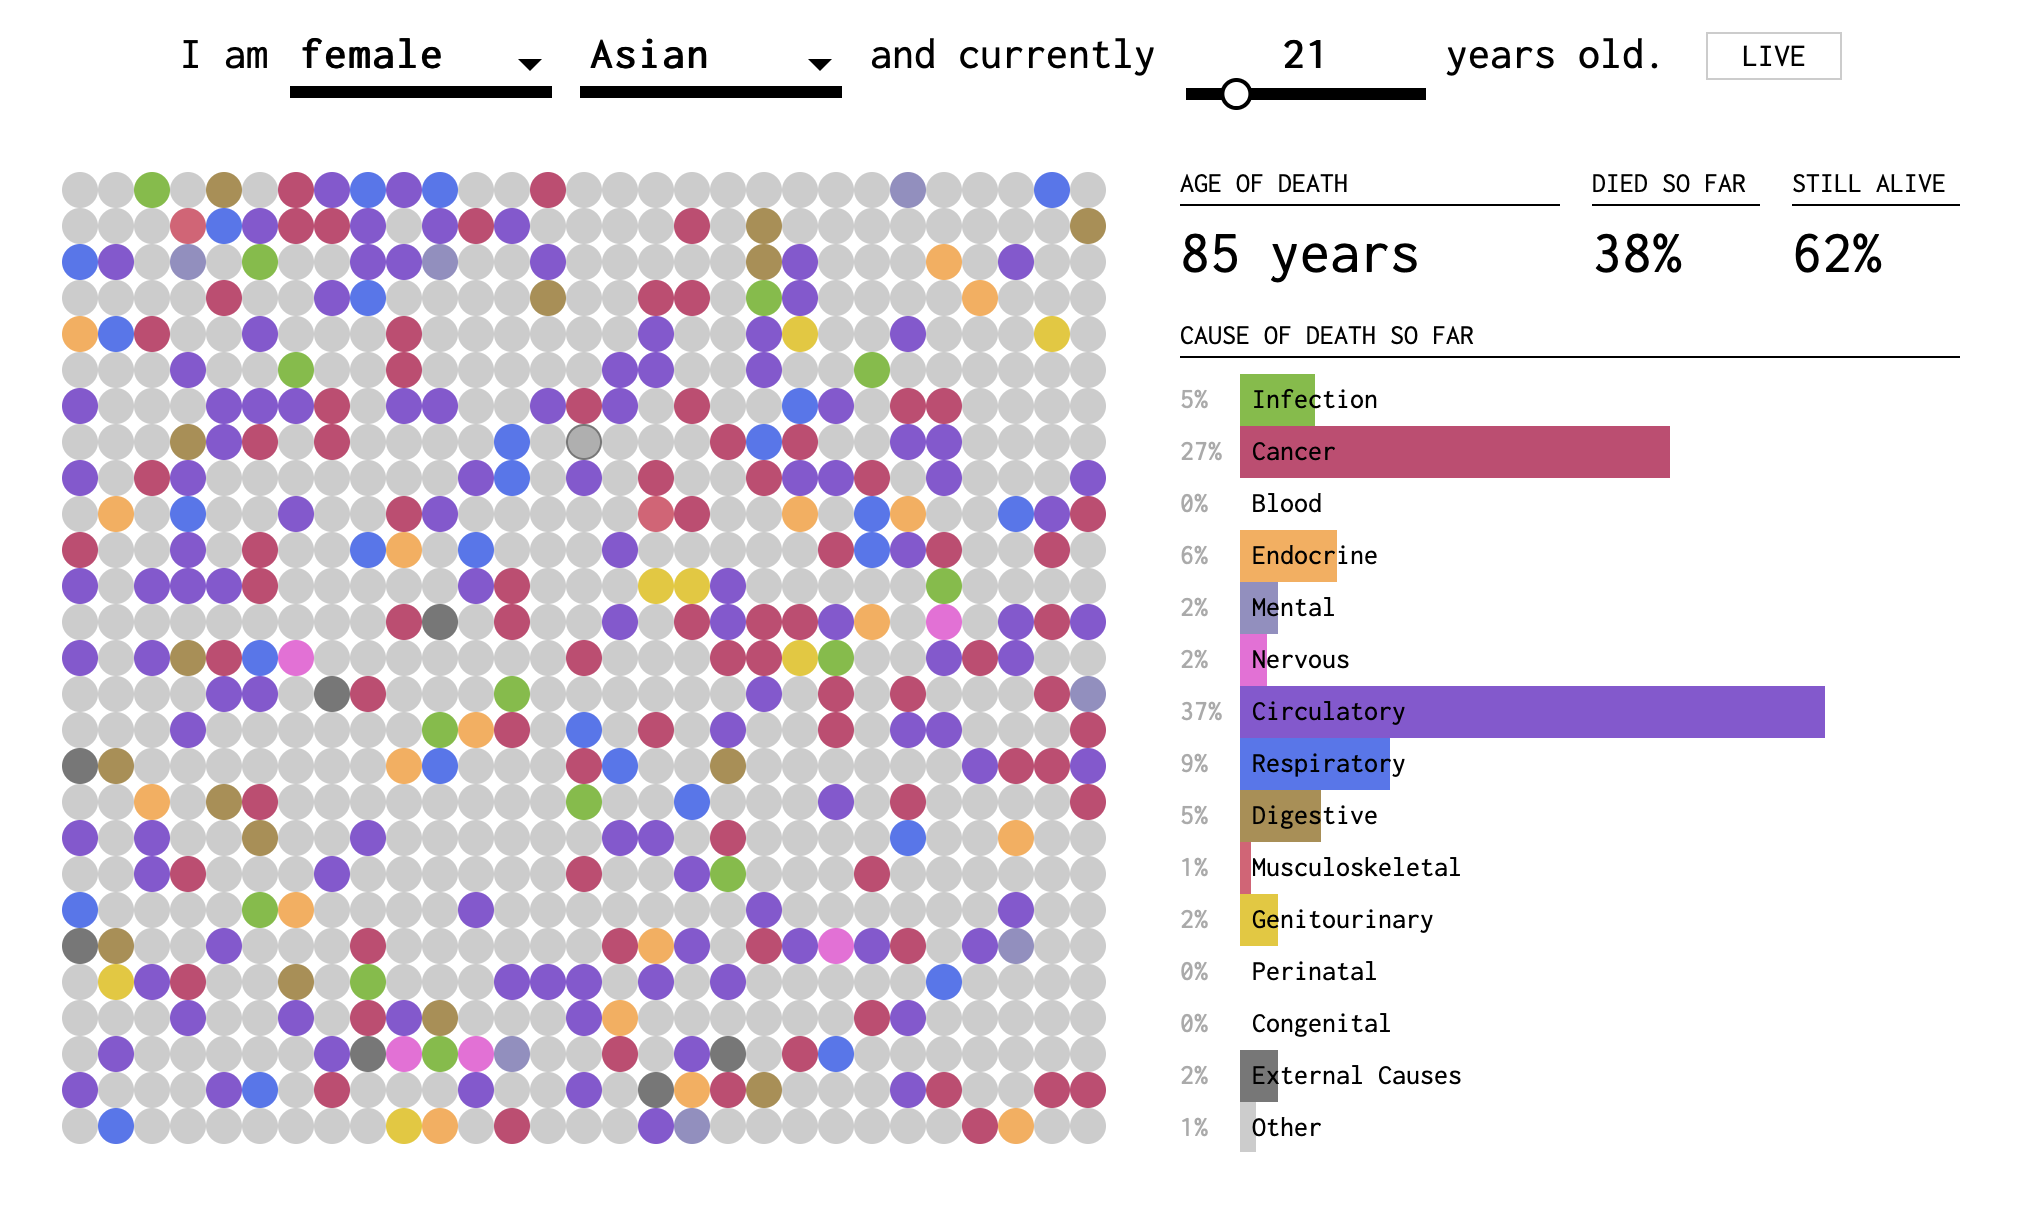
\includegraphics[width=0.8\linewidth]{images/HowYouWillDie21-85} 

}

\caption{Screenshot 2 of How You Will Die visualization}\label{fig:how-die-21-2}
\end{figure}

\begin{figure}

{\centering 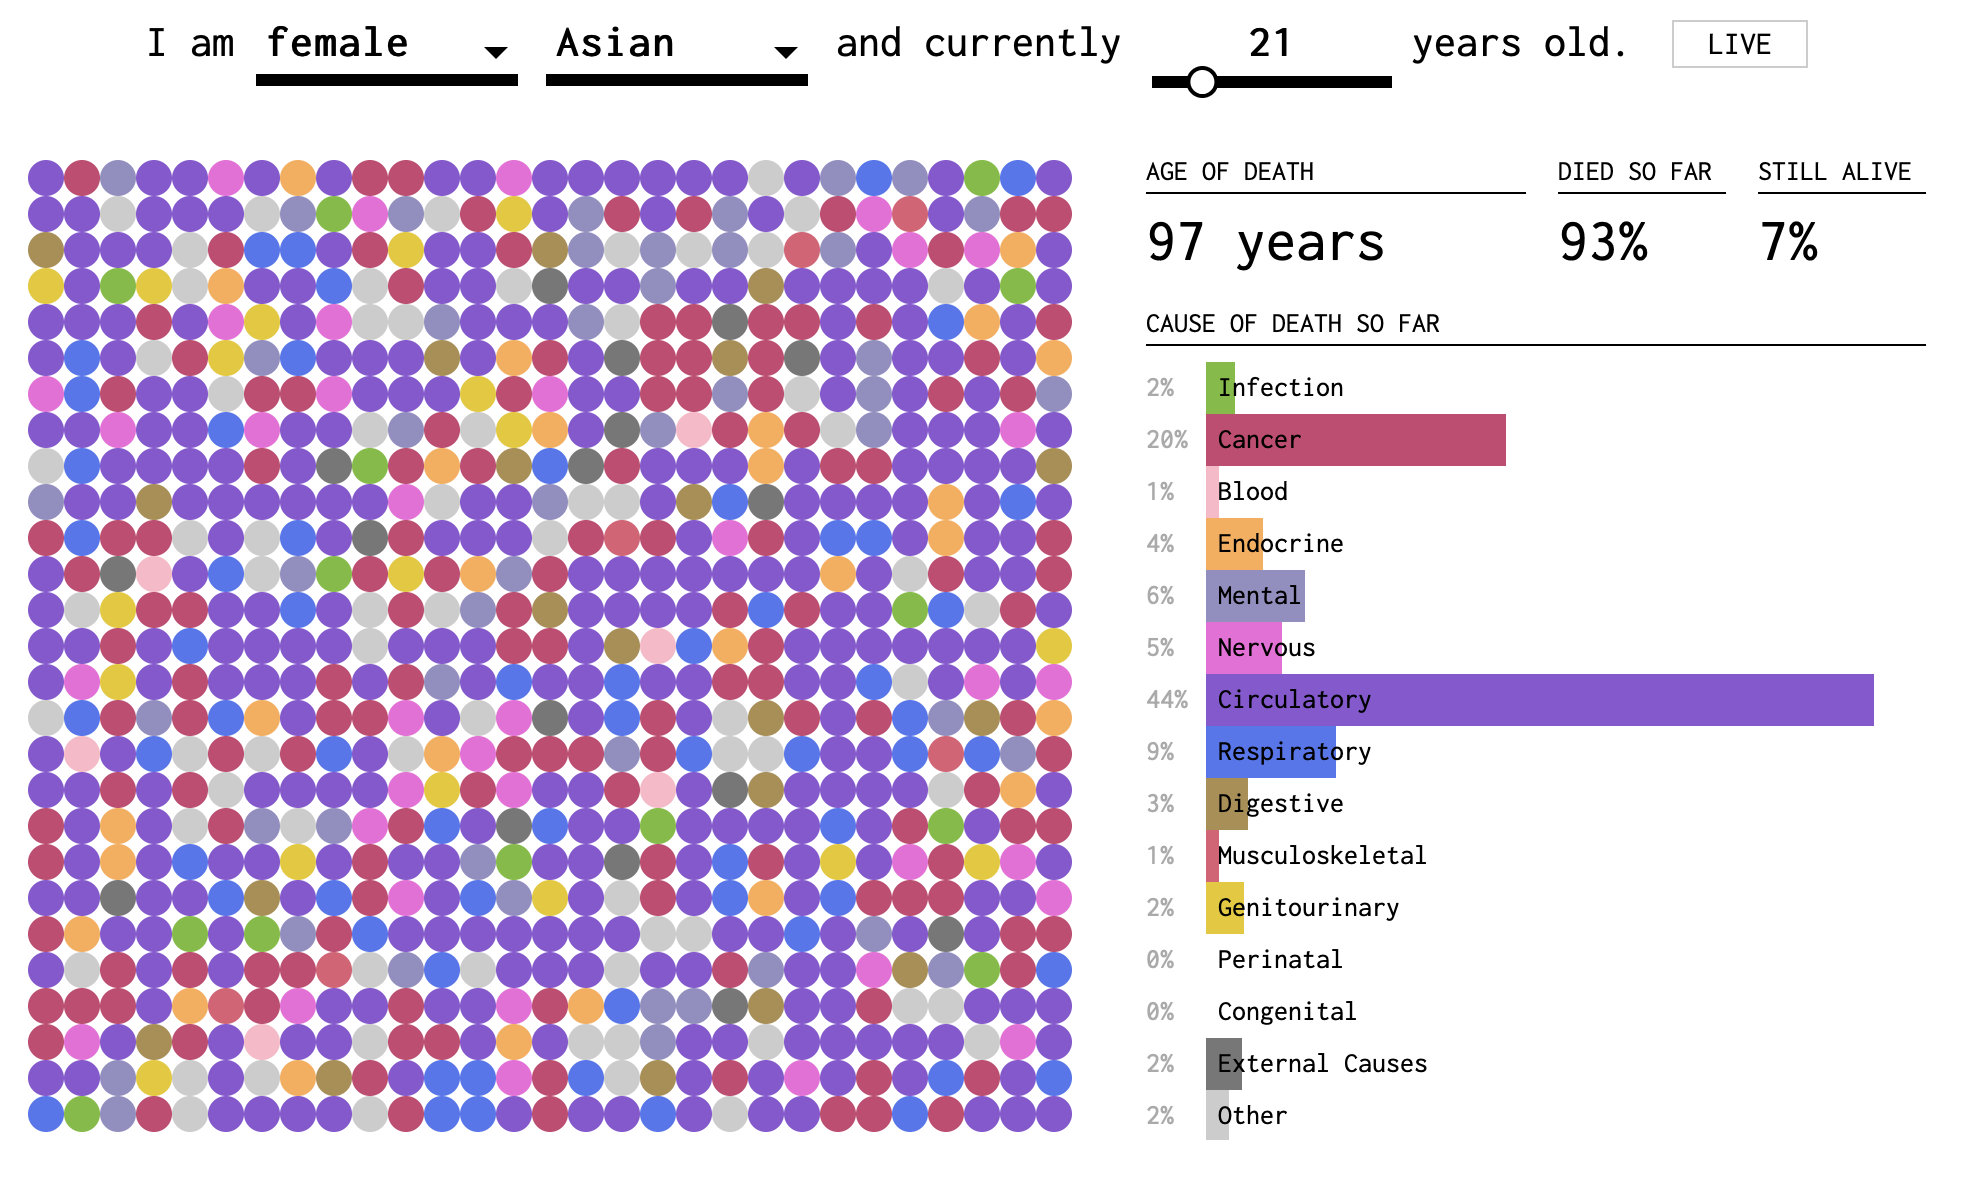
\includegraphics[width=0.8\linewidth]{images/HowYouWillDie21-97} 

}

\caption{Screenshot 3 of How You Will Die visualization}\label{fig:how-die-21-3}
\end{figure}

In this visualization, you can tell that death becomes more probable (and eventually certain) as you get older. The dots fill up slowly (except at the very beginning, when early childhood disease can play a role) and then more quickly. The colors represent causes. In the two-dimensional plane of dots, we get a sense of the randomness of the draw. But we also perceive the relative importance of causes by the areas taken up by purple and red. These are collected into a bar plot on the right side. At the base of each bar, the proportion is reported as a percentage of all deaths by this age.

\hypertarget{hold-my-beer}{%
\section*{Hold my beer}\label{hold-my-beer}}
\addcontentsline{toc}{section}{Hold my beer}

So far, we have conditioned on things that you can't change, like your age, race, or sex-at-birth. But what if I tell you that I'm about to do something really \sout{stupid} risky. Like suppose I told you I was going to eat a bunch of Pop Rocks and drink a lot of Coke, which we all know killed Little Mikey, the child star from the Life cereal commercials?\footnote{Okay, yeah, this is an urban legend: \url{https://www.snopes.com/fact-check/pop-rocks-soda/}}

If I am about to engage in highly risky behavior, you might not want to put the probability that I die this year at the 1\% or 2\% base rate from the life tables. You might think I have a 37\% chance of dying from an exploded stomach. Which, by the way, is an external cause. So you might think that the conditional probability of death \emph{by external causes} should go up, but not the probability of death by respiratory disease.

When there is something that you can change, or manipulate, such as engaging in a particular behavior (e.g., driving, rock climbing, or eating Pop Rocks and Coke), then we can imagine what \emph{might} have happened if you didn't do something that you did (or did something that in reality you didn't do). This is what is known as a \emph{counterfactual} claim, such as ``if I didn't check my email this morning before leaving the house, I would not have missed the train.'' Maybe. But how can we know?

Our knowledge about the world is based on a combination of observations. (I am distinguishing knowledge from belief, but epistemology is a big topic and beyond our scope at the moment!) Some of those observations are of the form where we do not deliberately manipulate conditions in the world, such as treatments, behaviors, or environmental factors. We just observe the joint occurrences of events in samples, such as health outcomes, behaviors, pollution levels, etc. Analysis of these kinds of data are called observational studies. We can also do experiments, sometimes, where we gather a sample of people and assign half of them to do something (e.g., take medicine, or sleep in a cabin) and half of them to do something else (e.g., take a placebo, or watch an informational video). These are experimental studies.

It is often said that experimental studies are the best way to develop knowledge about causation, that is, answers to questions of the form, does A cause B? Does eating meat cause heart disease? Does smoking cause lung cancer? And are experiments the only way to answer such questions?

What does it mean to say A causes B? The philosopher David Hume was one of the first to shed light on the question of how we conceive of causation. In the past twenty years, statistical thinking about causality has also changed a lot. In this course, we are going to take a pragmatic approach and focus on how we use the concept of causation in everyday life. It will be helpful to review our distinction between deterministic and stochastic processes and between associated and independent events.

\hypertarget{non-deterministic-causation}{%
\section*{Non-deterministic Causation}\label{non-deterministic-causation}}
\addcontentsline{toc}{section}{Non-deterministic Causation}

If I hit a porcelain tea cup hard with hammer and the tea cup breaks, we can safely say that hitting the teacup with a hammer caused the cup to break. We don't really feel the need to say that if you hit a teacup hard with a hammer, there is a 99.9997\% chance that it will break. Even if that's actually true. And we don't feel the need to define ``hard'' in this case either. We use an example like a teacup and hammer when we want to focus on the common-sense big picture and not the details. And the big picture here says that hitting a teacup with a hammer deterministically causes the teacup to break. Let us also assert that if we do not hit the teacup, and it just sits there, then it will not spontaneously break. In the case of the physics of hammers and teacups, we feel that we know this much is true.

What about buying a lottery ticket? Does buying a lottery ticket cause one to win the lottery? Well, you certainly are not guaranteed to win the lottery if you buy a ticket. (In fact, your chances will be very low. The subject of making money is the next Big Question). But you can't possibly win if you don't buy a ticket. So, strictly speaking, buying a ticket does influence the probability of winning.

We've now discussed two examples. In the first case (hammer and teacup):

\begin{itemize}
\tightlist
\item
  If A (hammer hits teacup) then definitely B (teacup breaks)
\item
  If not A (hammer does not hit teacup) then definitely not B (teacup does not break)
\end{itemize}

In table form:

\begin{longtable}[]{@{}lcc@{}}
\toprule()
& Teacup breaks & Teacup doesn't break \\
\midrule()
\endhead
Hammer hits teacup & Always* & Never \\
Hammer does not hit teacup & Never & Always \\
\bottomrule()
\end{longtable}

*pretty much; we're not splitting hairs here.

In the second case (lottery ticket):

\begin{itemize}
\tightlist
\item
  If A (buy lottery ticket) then maybe B (win lottery) and maybe not B (do not win lottery)
\item
  If not A (do not buy lottery ticket) then definitely not B (do not win lottery)
\end{itemize}

\begin{longtable}[]{@{}lcc@{}}
\toprule()
& Win lottery & Do not win lottery \\
\midrule()
\endhead
Buy lottery ticket & Rarely & Probably \\
Do not buy ticket & Never & Always \\
\bottomrule()
\end{longtable}

What about this question: does smoking cause cancer? Does it fit either of these two cases? Unfortunately the question about smoking does not. It belongs to a yet another case.

In the third case (smoking):

\begin{itemize}
\tightlist
\item
  If A (smoke) then maybe B (cancer) and maybe not B (no cancer)
\item
  If not A (do not smoke) then maybe B (cancer) and maybe not B (no cancer)
\end{itemize}

\begin{longtable}[]{@{}lcc@{}}
\toprule()
& Get cancer & Do not get cancer \\
\midrule()
\endhead
Smoke & Maybe & Maybe \\
Do not smoke & Maybe & Maybe \\
\bottomrule()
\end{longtable}

Now I'm not saying that the chances of cancer are the same whether you smoke or not. That remains an open question so far as our present argument goes. But even thus far, we can see that the smoking causality question, posed this way, invites some more questions.

How big a difference does there have to be between the cancer rates for smokers and non-smokers for us to be convinced that there is an association between smoking and cancer? And if there is an association between smoking and cancer, what would drive us to call this a causal relationship, to say that smoking causes cancer? Could there be a third variable? Could causality go the other way?

At minimum, we may say that there is no causation without association. If two events are independent (that is, they co-occur with frequencies that are consistent with their being independent events), then it does not make sense to say that one causes the other.

\hypertarget{testing-for-an-association-between-two-variables}{%
\section*{Testing for an association between two variables}\label{testing-for-an-association-between-two-variables}}
\addcontentsline{toc}{section}{Testing for an association between two variables}

Let's focus on the first question: How big a difference does there have to be between the cancer rates for smokers and non-smokers for us to be convinced that there is an association between smoking and cancer? Our approach to answering this question will be very similar to the one we used in Chapter \ref{test-indep} where we were considering associations between two-types-of-people questions. The method for establishing association is quite general.

Caveat: we are going to vastly oversimplify the problem here and use made up numbers. Smoking is not a dichotomous variable. People can smoke more or less heavily and for different durations. They may have already quit or be active smokers. For this worked example, we will imagine that we are sampling people between the ages of 50 and 75. We will operationalize smokers as heavy smokers: people who smoked the equivalent of at least 10 cigarettes a day for at least 20 years.

Suppose that we are able to obtain a randomly selected sample of 1000 people in this age group. For each one, the following information is available: a) whether the person is/was a heavy smoker and b) whether the person has ever been diagnosed with cancer. The beginning of our dataset might look something like this:

\begin{longtable}[]{@{}lcc@{}}
\toprule()
& Cancer? & Smoke? \\
\midrule()
\endhead
Person 1 & No & No \\
Person 2 & No & Yes \\
Person 3 & Yes & No \\
Person 4 & No & No \\
Person 5 & No & Yes \\
Person 6 & Yes & Yes \\
\bottomrule()
\end{longtable}

As a first step, you tabulate the data and get the following contingency table:

\begin{longtable}[]{@{}lcc@{}}
\toprule()
& Cancer: Yes & Cancer: No \\
\midrule()
\endhead
Smoke: Yes & 46 & 204 \\
Smoke: No & 93 & 657 \\
\bottomrule()
\end{longtable}

Then, you use the table to estimate the following:

\[P(\text{Cancer}|\text{Smoke})=\frac{46}{46+204}=0.184\]

\[P(\text{Cancer}|\text{Not Smoke})=\frac{93}{93+657}=0.124\]

You might say that these numbers suggest an association (i.e., dependence) between smoking and cancer: Within this sample, a higher proportion of smokers were diagnosed with cancer than non-smokers. But is this enough of a difference to convince you that, if you went out and found 1000 new (random) people, you would still observe a difference of this magnitude?

One way to \emph{start} trying to answer this question is to consider the following thought experiment: imagine that, among all people in the world, there is NOT a higher incidence of cancer among smokers (as compared to non-smokers). If that were the case, you would expect to see

\[P(\text{Cancer}|\text{Smoke})=P(\text{Cancer}|\text{Not Smoke}).\]

Or, written slightly differently:

\[P(\text{Cancer}|\text{Smoke})-P(\text{Cancer}|\text{Not Smoke})=0.\]

In comparison, you observed the following in your sample:

\[P(\text{Cancer}|\text{Smoke})-P(\text{Cancer}|\text{Not Smoke})=0.184-0.124=0.06.\]

So, you could pose the following question: what is the probability that, among the whole population, smokers do not have higher risk of cancer; but, among the random sample of 1000 people that you observed, there is a 6\% (or greater) increased incidence of cancer among smokers as compared to non-smokers? This type of question is the basis for \textbf{hypothesis testing}. Often, in hypothesis testing, we form a \textbf{null hypothesis} (in this case, the null hypothesis might be that smokers and non-smokers have equal cancer incidence among the full population) and \textbf{alternative hypothesis} (in this case, the alternative hypothesis might be that smokers have at least 6\% higher risk of cancer than non-smokers).

Based on the sample you observed, you could estimate that approximately \(\frac{46+204}{1000}*100=25\) percent of the population smokes and approximately \(\frac{46+93}{1000}*100=13.9\) percent of the population has been diagnosed with cancer. If there is no real difference in cancer incidence among smokers and non-smokers, then these two variables are independent: as though 25\% of your sample randomly decided to smoke, and 13.9\% were randomly diagnosed with cancer.

It is easy to simulate datasets under this assumption. In two completely separate (independent) steps, we will randomly assign to each of our 1000 people, a 25\% chance of being a heavy smoker and a 13.9\% chance of getting cancer. In Chapter \ref{test-indep}, we imagined starting with a fixed number of responses (e.g., smoker/non-smoker), shuffling those responses, and then redistributing the values among our virtual subjects. The code below actually does something different. It will draw values with replacement for each of the two variables. This means that in each replication, we will not actually have exactly 250 smokers and 139 cancers. The numbers will fluctuate somewhat in each simulated dataset.

After we generate our simulated datasets, we can calculate \(P(\text{Cancer}|\text{Smoke})-P(\text{Cancer}|\text{Not Smoke})\) and observe what range of values occurs. We will be particularly interested in the proportion of the time that this difference is greater than or equal to \(0.06\). That was our observed value. And in this simulation, we know that the two variables are independent. Thus, we are quantifying the chance of observing such a difference in outcomes due to random chance.

\begin{Shaded}
\begin{Highlighting}[]
\FunctionTok{set.seed}\NormalTok{(}\DecValTok{5123}\NormalTok{)}

\CommentTok{\#set some number of iterations/replications}
\NormalTok{nIter }\OtherTok{=} \DecValTok{100}

\CommentTok{\#create vector to save differences in proportions}
\NormalTok{differences }\OtherTok{=} \FunctionTok{vector}\NormalTok{(}\AttributeTok{length =}\NormalTok{ nIter) }
\ControlFlowTok{for}\NormalTok{(i }\ControlFlowTok{in} \DecValTok{1}\SpecialCharTok{:}\NormalTok{nIter)\{ }\CommentTok{\#repeat the following process nIter times}

  \CommentTok{\#create some fake data and save it as "fakedata"}
\NormalTok{  fakedata }\OtherTok{=} \FunctionTok{data.frame}\NormalTok{(}\AttributeTok{Smoke =} \FunctionTok{sample}\NormalTok{(}\FunctionTok{c}\NormalTok{(}\StringTok{"Y"}\NormalTok{, }\StringTok{"N"}\NormalTok{), }\AttributeTok{size=}\DecValTok{1000}\NormalTok{, }
                                       \AttributeTok{prob=}\FunctionTok{c}\NormalTok{(.}\DecValTok{25}\NormalTok{, .}\DecValTok{75}\NormalTok{), }\AttributeTok{replace =}\NormalTok{ T),}
                        \AttributeTok{Cancer =} \FunctionTok{sample}\NormalTok{(}\FunctionTok{c}\NormalTok{(}\StringTok{"Y"}\NormalTok{, }\StringTok{"N"}\NormalTok{), }\AttributeTok{size=}\DecValTok{1000}\NormalTok{, }
                                        \AttributeTok{prob=}\FunctionTok{c}\NormalTok{(.}\DecValTok{139}\NormalTok{, .}\DecValTok{861}\NormalTok{), }\AttributeTok{replace =}\NormalTok{ T))}

  \CommentTok{\#use the fake data to calculate P(cancer|smoke)}
\NormalTok{  CgivenS }\OtherTok{=} \FunctionTok{table}\NormalTok{(fakedata)[}\DecValTok{2}\NormalTok{,}\DecValTok{2}\NormalTok{]}\SpecialCharTok{/}\FunctionTok{sum}\NormalTok{(}\FunctionTok{table}\NormalTok{(fakedata)[}\DecValTok{2}\NormalTok{,])}

  \CommentTok{\#use the fake data to calculate P(cancer|not smoke)}
\NormalTok{  CgivenNS }\OtherTok{=} \FunctionTok{table}\NormalTok{(fakedata)[}\DecValTok{1}\NormalTok{,}\DecValTok{2}\NormalTok{]}\SpecialCharTok{/}\FunctionTok{sum}\NormalTok{(}\FunctionTok{table}\NormalTok{(fakedata)[}\DecValTok{1}\NormalTok{,])}

  \CommentTok{\#save P(cancer|smoke) {-} P(cancer|not smoke) in the ith location of differences}
\NormalTok{  differences[i] }\OtherTok{\textless{}{-}}\NormalTok{ CgivenS }\SpecialCharTok{{-}}\NormalTok{ CgivenNS}
\NormalTok{\}}

\CommentTok{\#calculate proportion of differences greater than or equal to .06}
\NormalTok{propGreater }\OtherTok{\textless{}{-}} \FunctionTok{sum}\NormalTok{(differences }\SpecialCharTok{\textgreater{}=}\NormalTok{ .}\DecValTok{06}\NormalTok{)}\SpecialCharTok{/}\NormalTok{nIter}

\CommentTok{\#plot a histogram of the differences with a red vertical line at .06}
\FunctionTok{hist}\NormalTok{(differences, }\AttributeTok{main=}\StringTok{"Histogram of P(cancer|smoke) {-} P(cancer|not smoke)"}\NormalTok{,}
     \AttributeTok{xlim=}\FunctionTok{c}\NormalTok{(}\SpecialCharTok{{-}}\FloatTok{0.1}\NormalTok{,}\FloatTok{0.1}\NormalTok{), }\AttributeTok{breaks=}\FunctionTok{seq}\NormalTok{(}\SpecialCharTok{{-}}\FloatTok{0.1}\NormalTok{,}\FloatTok{0.1}\NormalTok{,}\FloatTok{0.01}\NormalTok{))}
\FunctionTok{abline}\NormalTok{(}\AttributeTok{v=}\NormalTok{.}\DecValTok{06}\NormalTok{, }\AttributeTok{lwd=}\DecValTok{2}\NormalTok{, }\AttributeTok{col=}\DecValTok{2}\NormalTok{)}
\FunctionTok{text}\NormalTok{(}\FloatTok{0.09}\NormalTok{, nIter}\SpecialCharTok{/}\DecValTok{10}\NormalTok{, }\FunctionTok{paste0}\NormalTok{(propGreater}\SpecialCharTok{*}\DecValTok{100}\NormalTok{,}\StringTok{"\% of cases"}\NormalTok{))}
\end{Highlighting}
\end{Shaded}

\begin{center}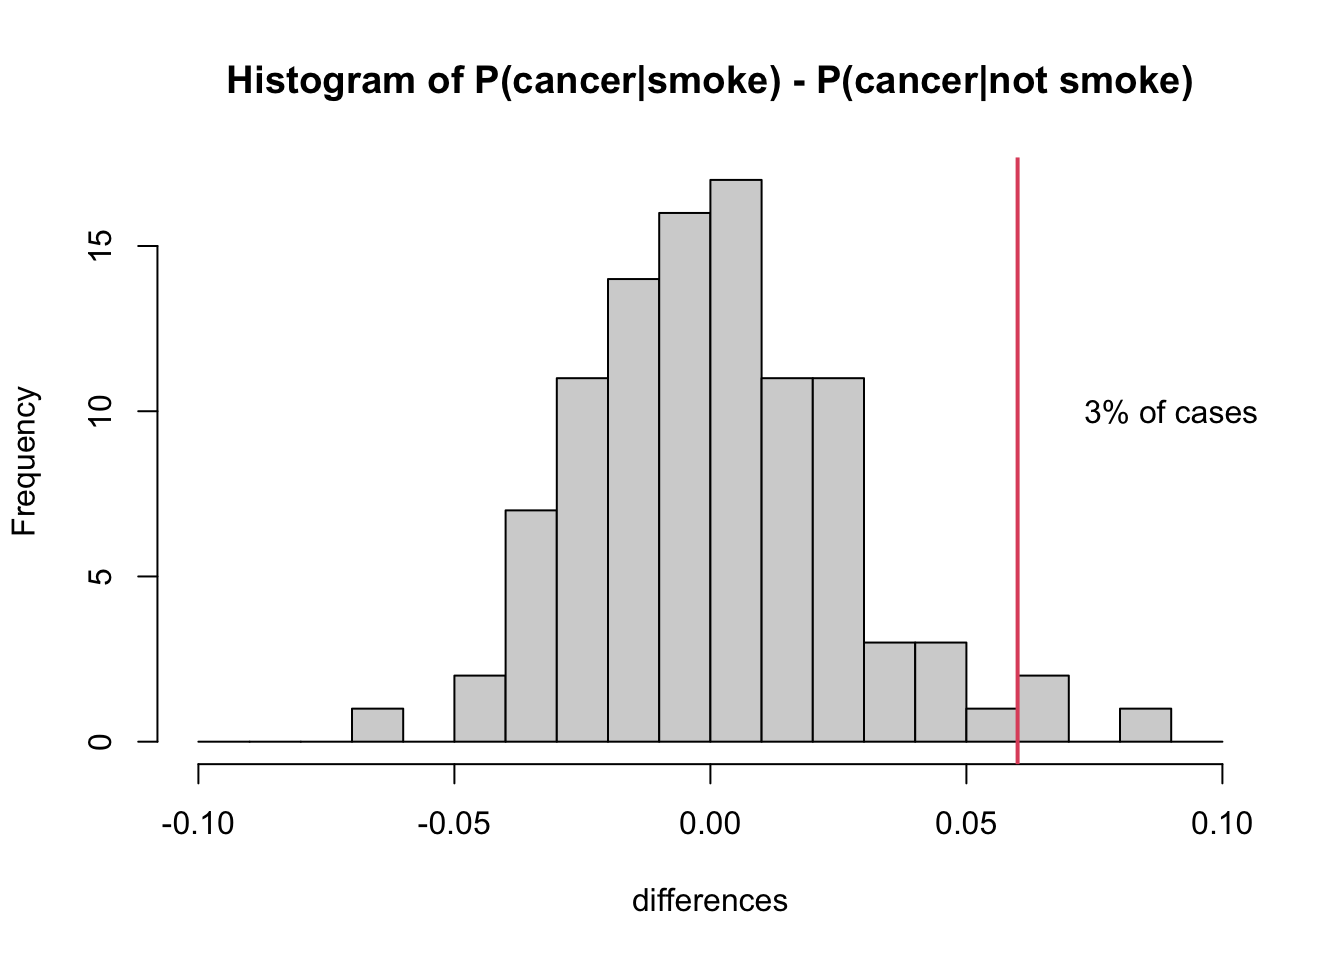
\includegraphics[width=0.9\linewidth]{carpedatum_files/figure-latex/unnamed-chunk-20-1} \end{center}

As you might expect, the histogram of simulated differences (\(P(\text{Cancer}|\text{Smoke}) - P(\text{Cancer}|\text{Not Smoke})\)) is centered around zero. If there's no real difference, then you should expect to observe (close to) zero differences among any random sample of 1000 people. That said, you'll see from the histogram that it is still possible, by random chance, to observe a difference as large or greater than 6\%.

In fact, in our simulation, this happened 3 times (3\% of the time). Remember that our simulation was carried out assuming independence, in which case there should be no difference. So we might interpret our findings as follows: there is a relatively low probability of observing \(P(\text{Cancer}|\text{Smoke}) - P(\text{Cancer}|\text{Not Smoke})\ge .06\) in a sample of 1000 people if it were truly the case that this difference was zero.

\hypertarget{will-you-make-money}{%
\chapter*{Will You Make Money?}\label{will-you-make-money}}
\addcontentsline{toc}{chapter}{Will You Make Money?}

\begin{quote}
No one can win at roulette unless he steals money from the table while the croupier isn't looking.

--- Albert Einstein (possibly)
\end{quote}

The development of probability theory is historically linked to attempts to understand games of chance, especially ones in which money was involved (see for example, \href{http://sites.math.rutgers.edu/~cherlin/History/Papers2000/cheng.html}{here}). Sometimes betting money on an uncertain outcome falls under the name of gambling; other times it's dignified with the name investment or ``smart business decision.'' But regardless of the label, there are smarter and less smart ways to play money games.

\hypertarget{battle-of-the-bills}{%
\section*{Battle of the Bills}\label{battle-of-the-bills}}
\addcontentsline{toc}{section}{Battle of the Bills}

Let's recall a distinction we made earlier in this course about deterministic and stochastic, or random, processes. This time, we'll think about two different bets you make with your friend. In the first bet, you and your friend are debating whether it was Bill Paxton or Bill Pullman in the movie Apollo 13. To make the game interesting, you bet two dollars. You look it up on the internet, and find that it was indeed Paxton. One of you wins. Do you feel the need to check again? Probably not. This particular question, although you may not have known the answer for sure, has only one possible answer, no matter how many times you check.

Now consider another bet, this time for three bucks! You and your friend are walking down the street debating the ``merits'' of mint chocolate chip vs.~cookies and cream as ice cream flavors. You claim that mint chocolate chip is the more popular flavor, and decide to ask the first passer-by which flavor they think is better. Suppose they don't just ignore you, thinking you're a nutcase, and they answer cookies and cream. Are you satisfied with this one answer? Or do you feel the need to ask another pedestrian? And how many?

We might say that the variable ``BPA'', which stands for ``which Bill P. starred in Apollo 13?'' has a deterministic answer. It is always the same. But the variable ``MCCoCAC'' which stands for ``mint chocolate chip \textgreater{} cookies and cream?'' can take on different answer (one of two; no ties allowed) depending on whom we ask. Because it is a random or stochastic variable, we have to talk about it using different terms. We might say something like, what proportion of people (in this neighborhood, say) prefer cookies and cream? Or what are the chances that the first person we ask will express that particular preference.

This may all sound like silly bets that are really just games between friends. But people make small and large money bets all the time, in everything from business and life decisions, to recreational games. In this module, we explore probability calculations that inform things like advertising, airplane booking, the job market, and march madness.

\hypertarget{betting-on-beer-or-ice-cream}{%
\chapter{Betting on Beer (or Ice Cream)}\label{betting-on-beer-or-ice-cream}}

This section makes reference to Chapter 5 of Naked Statistics by Charles Wheelan.

In 1981, Schlitz brewing company, now defunct but at one time the largest beer producer in the US, ran a bold advertising campaign. During the Super Bowl, Schlitz ran a live blind taste test against one of its competitors, Michelob. 100 Michelob drinkers participated in the taste test, which aired LIVE. The advertisement slot itself cost a lot of money. Schlitz could have just run a funny ad involving puppies on the beach, so why take a risk with a taste test that could conceivably have gone badly. How could Schlitz have been so confident that their beer would be preferred?

\begin{quote}
THINK ABOUT IT QUESTION: What information would you need to know to advise the Schlitz brewing company about running such an ad? (Take a few minutes before continuing on, to try to list this information on your own).
\end{quote}

As discussed in Wheelan's chapter, some things we would need to know are:

\begin{itemize}
\tightlist
\item
  Actual proportion of Michelob drinkers who would prefer Schlitz in a blind taste test
\item
  Acceptable outcome of live taste test for promoting Schlitz beer
\item
  Intended sample size for taste test
\item
  Rules of mathematical probability
\end{itemize}

Wheelan adds a lot of context to this particular story, which is part of the fun. In particular, he asserts that Schlitz and Michelob are probably indistinguishable to most beer drinkers. This puts the chances of anyone prefering one beer over the other at 50\%. He also points out that the marketing campaign works well for a range of outcomes, because the taste test is conducted with Michelob drinkers. Schlitz executives will be quite happy to be able to say that even 40\% of Michelob drinkers prefer Schlitz, which sounds (and is) very different from saying that 40\% of all beer drinkers prefer Schlitz over Michelob.

Wheelan invokes the ``law of large numbers'' to argue that for a given sample size, and if the actual proportion is 50\%, that the results of the live taste test can be almost guaranteed to be satisfactory for Schlitz (we define satisfactory, for now, as at least 40\% preferred). The larger the sample size, the greater the probability that the taste test will be a success. We have created a \href{https://ybergner.shinyapps.io/Schlitz/}{Schlitz simulation} for you to explore this for yourself.

In his book, Wheelan claims that (a) for 10 blind tast testers, the probability of a happy outcome is 0.83 and (b) for 100 blind taste testers, the probability is 0.98. If you don't want to take this assertion at face value, you might try convincing yourself by opening the simulation, running 100 simulated experiments of sample size 10 or 100, and inspecting the proportion of those experiments that led to a favorable outcome. You should see values around .83 and .98 for sample sizes of 10 and 100, respectively.

For a moment, let's pull back the curtain on the Schlitz simulation and see how it works. The following code walks through the process of repeatedly surveying 10 people, recording the proportion who preferred Schlitz (under the assumption that each person has a 50\% chance of preferring Schlitz), and calculating the proportion of those 10-person surveys that led to an acceptable outcome. If we collect 10,000 samples of 10 people and calculate the proportion of those 10 person samples where at least 4 out of 10 people preferred Schlitz, we can estimate the probability of an acceptable outcome very accurately:

\begin{Shaded}
\begin{Highlighting}[]
\NormalTok{numExpts }\OtherTok{=} \DecValTok{10000} \CommentTok{\#set some number of repeated experiments to run}
\NormalTok{sampleSize }\OtherTok{=} \DecValTok{10} \CommentTok{\#set the sample size  }
\NormalTok{trueProb }\OtherTok{=}\NormalTok{ .}\DecValTok{5} \CommentTok{\#set the (true) probability of preferring Schlitz}
\NormalTok{acceptableOutcome }\OtherTok{=}\NormalTok{ .}\DecValTok{4} \CommentTok{\#set an acceptable proportion of Schlitz preferrers}

\NormalTok{results }\OtherTok{=} \FunctionTok{vector}\NormalTok{(}\AttributeTok{length =}\NormalTok{ numExpts) }\CommentTok{\#create a vector of length nIter}

\ControlFlowTok{for}\NormalTok{(i }\ControlFlowTok{in} \DecValTok{1}\SpecialCharTok{:}\NormalTok{numExpts)\{ }\CommentTok{\#repeat the following process numExpts times}
   \CommentTok{\#Choose sampleSize{-}many values from the set (0,1) with replacement}
   \CommentTok{\#where the probability of drawing a 1 is equal to trueProb}
   \CommentTok{\#save the results in a vector called drawResults}
\NormalTok{   drawResults }\OtherTok{=} \FunctionTok{sample}\NormalTok{(}\FunctionTok{c}\NormalTok{(}\DecValTok{0}\NormalTok{,}\DecValTok{1}\NormalTok{), }\AttributeTok{size=}\NormalTok{sampleSize, }\AttributeTok{prob=}\FunctionTok{c}\NormalTok{(}\DecValTok{1}\SpecialCharTok{{-}}\NormalTok{trueProb, trueProb), }\AttributeTok{replace=}\ConstantTok{TRUE}\NormalTok{)}
   
   \CommentTok{\#In the ith location of "results", calculate the proportion of 1s in Samp}
\NormalTok{   results[i] }\OtherTok{=} \FunctionTok{sum}\NormalTok{(drawResults)}\SpecialCharTok{/}\NormalTok{sampleSize}
   \CommentTok{\# NB: this would also have worked }
\NormalTok{\}}

\CommentTok{\#Calculate the proportion of random experiments that were "acceptable"}
\FunctionTok{sum}\NormalTok{(results }\SpecialCharTok{\textgreater{}=}\NormalTok{ acceptableOutcome)}\SpecialCharTok{/}\NormalTok{numExpts}
\end{Highlighting}
\end{Shaded}

\begin{verbatim}
## [1] 0.834
\end{verbatim}

Feel free to copy this code over into your own script in RStudio and play with the parameters to see what happens. If you decrease \texttt{numExpts} to 1000 and re-run the simulation a few times, you might see that there is more variation in the estimated probability; however, if you increase \texttt{numExpts} to 100000, you are more likely to observe values very close to .83 every time. That is, the sampling variance is larger for small samples and smaller for large samples.

\hypertarget{how-do-statisticians-solve-problems-like-this}{%
\section*{How do statisticians solve problems like this?}\label{how-do-statisticians-solve-problems-like-this}}
\addcontentsline{toc}{section}{How do statisticians solve problems like this?}

In this course, I have tried to emphasize conceptual understanding through simulation and discussion. In the example above, you can, for example, run a bunch of simulations of the experiment and (very accurately) estimate the probability of an acceptable outcome. But, you'll get slightly different answers each time you run the simulation. If this bothers you, read on.

Mathematical statistics does have precise answers that depend on properties of \textbf{continuous distributions} like the normal distribution and the binomial distribution. The term data distribution comes from trying to describe how data or observations are \emph{distributed} across the values that they can attain. For example, are all outcomes equally likely? (A uniform distribution.) Or are values near the ``middle'' more likely than values farther away? A histogram is one way to visualize a distribution, and we often speak of the ``shape of a distribution.'' The normal and binomial distributions (which are both bell-shaped, by the way) are idealizations that are realized if we have an infinite amount of data. In reality we only have finite samples.
But when we have large enough samples, even though they are not infinite, their data distributions start to look more and more like their idealized versions.

The Schlitz commercial is exactly the kind of scenario that is explained using a binomial distribution (more on that later). If we ran the simulation (always with samples of 10), taking more and more observations (i.e., 100 samples of 10, 1000 samples of 10, etc.) and checked our success rate (defined by at least 4/10 preferring Schlitz), we would see that indeed this proportion does converge. This is plotted in Figure \ref{fig:converge-binom}. The x-axis is the number of samples, but note that \textbf{the x-axis is shown using logarithmic scales}. We need to use this scale, or else all of the points at smaller values would be bunched together. (Try this at home: draw an x-axis and label one end 0 and the other end 100,000. Now try placing tick marks at the values 10, 100, 1000, and 10,000.)

\begin{figure}

{\centering 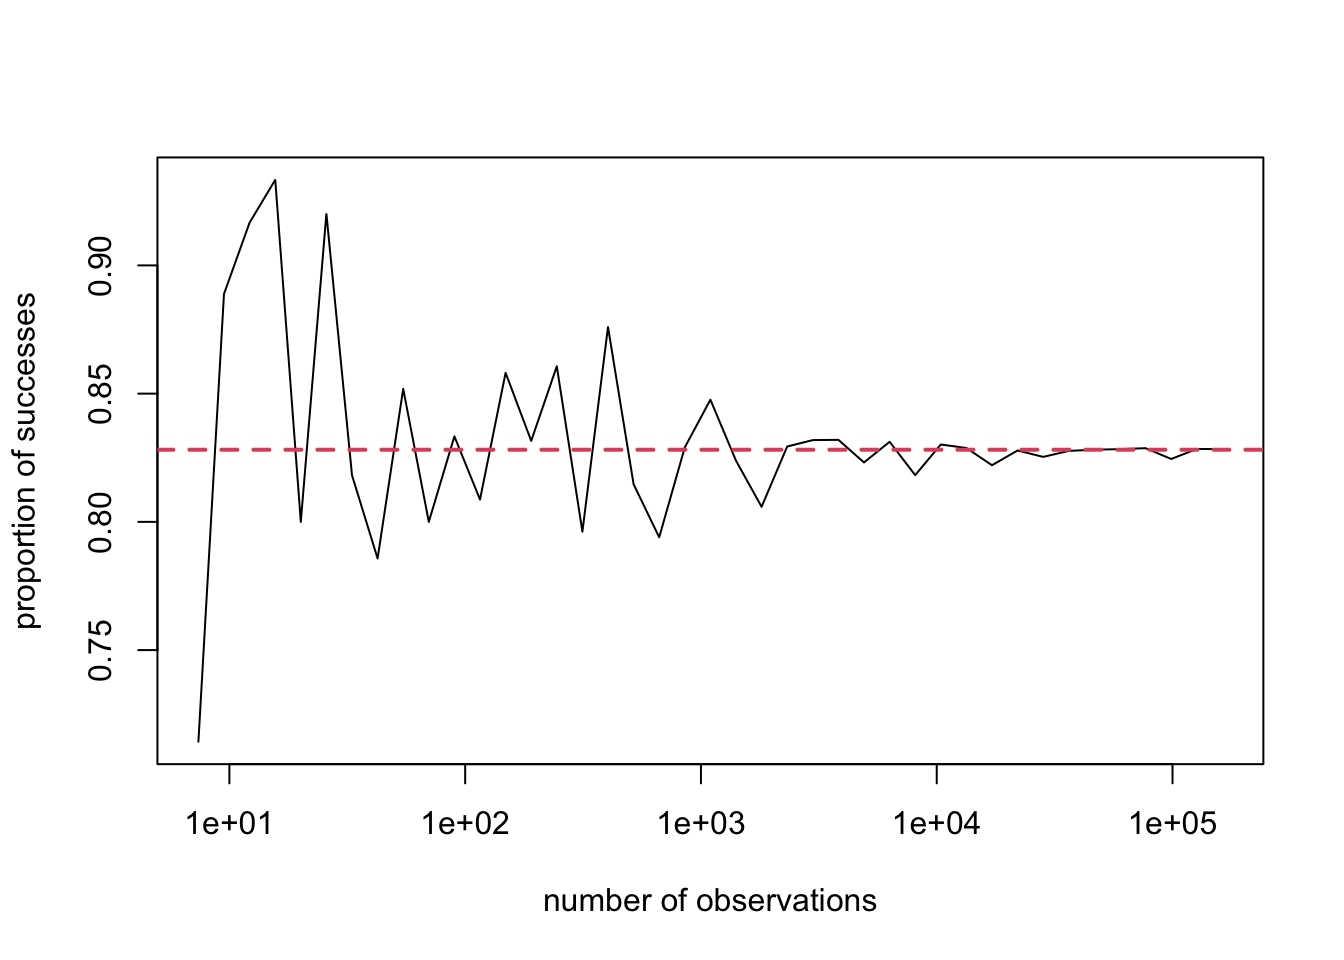
\includegraphics[width=0.9\linewidth]{carpedatum_files/figure-latex/converge-binom-1} 

}

\caption{Convergence of successful tasting proportions}\label{fig:converge-binom}
\end{figure}

So we see that there is some convergence: If we run more and more experiments, we find that the proportion of ``successful'' experiments converges to a stable value. But how can you calculate that value precisely? To find the analytical (i.e., exact) answer, instead of using a simulation to estimate it (empirically), it helps to start with a small sample size, say 2. Now that we've reduced our scope, we have some hope of writing all possible outcomes of this experiment and their probabilities.

What are all of the possible outcomes of 2 independent taste tests? We are using the word independent here, because we believe that one person's preference in a blind taste test does not influence the preference expressed by another person. If the same person were asked to do the taste test on two occasions, it might not be appropriate to treat those two results as independent. Unless the beers are truly indistinguishable. In any case, we are assuming that we have two strangers.

\begin{quote}
Aside: To be more precise, we should say that the two strangers' answers are \emph{conditionally independent}, because their preference does, in principle, reflect the quality of the beer. Suppose I told you that I had two beers, a horrible one and a delicious one. And that I was going to put them to a blind taste test. I don't tell you which is labeled beer A and whcih is beer B. I tell you that one person preferred beer A. Now another person comes to take the test. Which do you think they will pick? Probably beer A, because that one is probably the delicious one. So it looks like knowing what one person chose provides information about what the other one will choose. Which seems to violate the definition of independence. We can condition this association away. The answers are not causally associated, but rather indirectly associated by the fact that they are both explained by the ``true'' taste of the beer. That is our third, or lurking, variable here. I didn't tell you whether beer A or B was the delicious one. You tried guess which it is, based on the one observation of preference for beer A. However, if I told you that in fact beer B is the delicious one, but one out of twenty people seem to prefer beer A anyway, then this would change things. Knowing that one person came along and picked A would not make you predict that the next person will do the same. You will still, if you take my word for it, predict that the next person (and almost all of the people to come) will choose beer B. The formal way to put all of this together is that conditioning on the known desirability of the beer, each individual taste test is independent of the others. In the example above, we assumed that the chances are 50/50, but they didn't have to be for the conditional independence of trials to hold.
\end{quote}

There are two possibilities for each taster (either Schlitz or Michelob), so if we represent each possible outcome as (taster 1's choice, taster 2's choice), we get 4 possibilities.

\begin{verbatim}
{(Michelob, Michelob), (Michelob, Schlitz), (Schlitz, Michelob), (Schlitz, Schlitz)}
\end{verbatim}

The possible outcomes of a random experiment form a set, which is called the \textbf{sample space}. As per convention, we use curly brackets to indicate the set. The elements of the set are the outcomes, and we use ordinary parentheses to indicate the ordered pair of (Taster1, Taster2). At this point, you might find it helpful to look back at Chapter \ref{somefacts} to refresh your memory.

Because each individual taste test is independent, we already know how to express the (joint) probability of an outcome involving multiple tasters in terms of the individual probabilities.
For example, the probability of (Michelob, Schlitz) is:

\begin{verbatim}
P(Michelob, Schlitz) = P(taster 1 prefers Michelob AND taster 2 prefers Schlitz)
                     = P(taster 1 prefers Michelob) * P(taster 2 prefers Schlitz)
\end{verbatim}

If we assume that every taste tester is equally likely to prefer either beer, then

\begin{verbatim}
P(taster 1 prefers Michelob) = 0.5 = P(taster 2 prefers Schlitz)
\end{verbatim}

and so \texttt{P(Michelob,\ Schlitz)\ =\ \ (.5)*(.5)=.25}. In other words, there is a 25\% chance that the outcome of the experiment is that the first taster prefers Michelob and the second taster prefers Schlitz. In fact, assuming a 50\% chance of preferring either beer, we'll get the same probability for any of the four outcomes.

Notice that the four outcomes listed above are disjoint (only one can occur) and complete (one of them \emph{MUST} occur). Therefore, we also knew that their probabilities must add up to 1. And since they are also equiprobable, we could have known that each probability must by 0.25.

Now we can ask: which of the four possible outcomes will meet our requirement that at least 40\% of respondents prefer Schlitz? Probability textbooks often use the word \textbf{event} to describe some subset of the sample space for a random experiment. An event can be one outcome, a subset of one, but it can also span several outcomes. In this case, we could describe the event that at least 40\% of respondents prefer Schlitz as the set: Acceptable = \{(Michelob, Schlitz), (Schlitz, Michelob), (Schlitz, Schlitz)\}. If the probability of each outcome is 0.25, then because the outcomes are disjoint, the probability of ``Acceptable'' is

\begin{verbatim}
P(Acceptable) = P(Michelob, Schlitz) + P(Schlitz, Michelob) + P(Schlitz, Schlitz) 
                 =0.25 + 0.25 + 0.25 = 0.75
\end{verbatim}

Notice that because all of the outcomes are equally probably, the probability of an acceptable outcome reduces to the number of acceptable outcomes divided by the total number of possible outcomes. In this case, 3 out of 4, or 75\%.

\begin{quote}
Excercise: How would the probability of an acceptable outcome change if we believed that each taster had only a 40\% chance of preferring Schlitz (and a 60\% chance of preferring Michelob)?
\end{quote}

After all this work, you might be thinking: well that's all fine and good, but it's a lot of work to write out the sample space and list of acceptable outcomes for a sample size of 10 or even 100. You'd be right. For larger sample sizes, we need to employ some new techniques and R functions (which are only briefly covered in this text). But, for the sake of completeness, let's briefly examine two ways to conceptualize the problem and calculate the analytical probabilities in R. Don't worry if it doesn't make perfect sense yet; we won't make you do this by hand!

\hypertarget{the-solution-by-counting-or-combinatorics}{%
\subsection*{The solution by counting, or combinatorics}\label{the-solution-by-counting-or-combinatorics}}
\addcontentsline{toc}{subsection}{The solution by counting, or combinatorics}

First consider the simple case above, where tasters are equally likely to prefer Schlitz or Michelob. Because all individual probabilities are equal, all joint probabilities are equal---e.g., the probability of (Michelob, Michelob, Schlitz, Michelob) is the same as that of (Schlitz, Michelob, Schlitz, Michelob). We can calculate the probability of an acceptable outcome (at least 40\% preferring Schlitz) among 10 tasters by figuring out (i.e., counting) how many of the possible outcomes are acceptable outcomes. The total number of possible outcomes is \(2^{10}\) for a 10 person sample size (this is the same math as in the calculation of how many types of people you could observe by asking \(10\) independent, dichotomous questions).

One acceptable outcome would be if everyone chose Schlitz. But it would still be acceptable if 9/10 of the tasters chose Schlitz, and there are 10 different ways that could happen, because the Michelob chooser could be in position 1\ldots10 in the order. We are going to have to follow this logic down to 8, 7, 6, 5, and 4 out of 10 (since all would be acceptable). So we nned to dust off the old choose() function. If you've never seen it before: choose(n,k) (read ``n choose k'' and often written \(n\choose{k}\)) is the number of possible ways to choose k items out of a group of n total items. In this context, choose(n=10,k=4) is the number of unique groups of 4 tasters among a total pool of 10 tasters (i.e., number of ways that exactly 4/10 tasters could prefer Schlitz). In R:

\begin{Shaded}
\begin{Highlighting}[]
\CommentTok{\#calculate choose(n=10,k=4) in R}
\FunctionTok{choose}\NormalTok{(}\AttributeTok{n=}\DecValTok{10}\NormalTok{, }\AttributeTok{k=}\DecValTok{4}\NormalTok{)}
\end{Highlighting}
\end{Shaded}

\begin{verbatim}
## [1] 210
\end{verbatim}

\begin{Shaded}
\begin{Highlighting}[]
\CommentTok{\#calculate choose(n=10,k= all the numbers between 4 and 10)}
\FunctionTok{choose}\NormalTok{(}\AttributeTok{n=}\DecValTok{10}\NormalTok{, }\AttributeTok{k=}\DecValTok{4}\SpecialCharTok{:}\DecValTok{10}\NormalTok{)}
\end{Highlighting}
\end{Shaded}

\begin{verbatim}
## [1] 210 252 210 120  45  10   1
\end{verbatim}

\begin{Shaded}
\begin{Highlighting}[]
\CommentTok{\#add up all of the values above using sum() and then divide by 2\^{}10}
\FunctionTok{sum}\NormalTok{(}\FunctionTok{choose}\NormalTok{(}\AttributeTok{n=}\DecValTok{10}\NormalTok{, }\AttributeTok{k=}\DecValTok{4}\SpecialCharTok{:}\DecValTok{10}\NormalTok{))}\SpecialCharTok{/}\DecValTok{2}\SpecialCharTok{\^{}}\DecValTok{10}
\end{Highlighting}
\end{Shaded}

\begin{verbatim}
## [1] 0.828125
\end{verbatim}

\begin{quote}
Excercise: Can you modify the above code to calculate the empirical probability of an acceptable outcome for a sample size of 100 (again assuming preference for Schlitz and Michelob are equally likely)?
\end{quote}

\hypertarget{the-solution-by-distribution-or-statistics}{%
\subsection*{The solution by distribution, or statistics}\label{the-solution-by-distribution-or-statistics}}
\addcontentsline{toc}{subsection}{The solution by distribution, or statistics}

The above combinatoric method won't work if the outcomes are not equally probable. We may want to account for different probabilities of preferring Schlitz or Michelob. Maybe it's 43\% to 57\% and not 50/50.

Now we will need to call upon the powers of the binomial probability distribution. This function and its relatives can answer questions such as what is the probability of 42 successes in 89 independent trials, each of which has a 0.44 chance of being successful. Of course those numbers are arbitrary. In R, the function \texttt{dbinom(x,n,p)} gives the probability of \texttt{x} ``successes'' in \texttt{n} independent random trials, where each random trial has probability of success = \texttt{p}. For example, \texttt{dbinom(4,10,0.5)} is the probability that exactly 4 out of 10 people prefer Schlitz if the probability of any individual preferring Schlitz is 0.5. Using this function, we can now repeat the calculation above using some slightly different code:

\begin{Shaded}
\begin{Highlighting}[]
\CommentTok{\# calculate a few individual values, e.g., dbinom(4,10,.5)}
\FunctionTok{dbinom}\NormalTok{(}\DecValTok{4}\NormalTok{,}\DecValTok{10}\NormalTok{,}\FloatTok{0.5}\NormalTok{)}
\end{Highlighting}
\end{Shaded}

\begin{verbatim}
## [1] 0.2050781
\end{verbatim}

\begin{Shaded}
\begin{Highlighting}[]
\FunctionTok{dbinom}\NormalTok{(}\DecValTok{5}\NormalTok{,}\DecValTok{10}\NormalTok{,}\FloatTok{0.5}\NormalTok{)}
\end{Highlighting}
\end{Shaded}

\begin{verbatim}
## [1] 0.2460938
\end{verbatim}

\begin{Shaded}
\begin{Highlighting}[]
\FunctionTok{dbinom}\NormalTok{(}\DecValTok{6}\NormalTok{,}\DecValTok{10}\NormalTok{,}\FloatTok{0.5}\NormalTok{)}
\end{Highlighting}
\end{Shaded}

\begin{verbatim}
## [1] 0.2050781
\end{verbatim}

\begin{Shaded}
\begin{Highlighting}[]
\CommentTok{\#add up the probabilities of 4,5,6,7,8,9, or 10 people preferring Schlitz}
\FunctionTok{sum}\NormalTok{(}\FunctionTok{dbinom}\NormalTok{(}\DecValTok{4}\SpecialCharTok{:}\DecValTok{10}\NormalTok{,}\DecValTok{10}\NormalTok{,}\FloatTok{0.5}\NormalTok{))}
\end{Highlighting}
\end{Shaded}

\begin{verbatim}
## [1] 0.828125
\end{verbatim}

\begin{quote}
Exercise 1: Can you explain why choose(n=10, k=4)/2\^{}k is equal to dbinom(4,10,.5)?
\end{quote}

\begin{quote}
Exercise 2: Can you modify the code above to calculate the probability of an acceptable outcome if each taster only has a 40\% chance of preferring Schlitz?
\end{quote}

If these calculations feel a little overwhelming and confusing at this point, don't fear! Instead, revel in the fact that you just got (approximately) the same number using three different conceptualizations of the same problem. The point is: there are many ways to answer probabilistic questions, and simulation can be a powerful tool to side-step advanced probability calculations.

\hypertarget{expected-value}{%
\chapter{Expected Value}\label{expected-value}}

\hypertarget{betting-on-ice-cream}{%
\section*{Betting on ice cream}\label{betting-on-ice-cream}}
\addcontentsline{toc}{section}{Betting on ice cream}

The Schlitz example feels a bit contrived, at least to me, because in the scenario, the Schlitz executives don't really care about the truth. They just care about what will play well to Super Bowl audiences. Nevertheless, we can see the beer taste test as an example of a sampling procedure. We sample from a population (e.g., 100 beer drinkers) to make inferences about the whole population (100 beer drinkers).

You saw---using the simulation---that whenever you collect data from a sample, you get slightly different results. In this case, you observe a \textbf{sampling distribution} in the observed proportion of Schlitz-preference. It had that bell-shaped curve. I want to show you that the same simulation can be used to help you resolve your bet with your friend about whether most people prefer mint chocolate chip or cookies and cream as flavors of ice cream.

Let's now return to the ice cream bet that you made with your friend. Now some people just like to bet on any random event like dice rolls and wheel spins; we'll come back to gambling later. But when you bet your friend, it's often because you think you are right, but you acknowledge that you are uncertain. Your hunch is that the \emph{true} value of ice cream preference is greater than 50\% in favor of mint chocolate chip. By true value, I mean the answer you would get if you could literally ask everyone in the world this question or, to save time, if you could consult the all-knowing-one and just ask them. This conviction is important, because if both you and your friend believe the proportion really is 50/50, then you are just betting on a coin toss. Which is cool, if you want to do that.

Suppose you believe that the true value is 65\%. Just about two out of three people prefer mint chocolate chip. Your friend thinks the edge goes slightly to cookies and cream, but not enough to notice, and what's the point of betting on a coin toss. You want to make a point, though, so you're willing to go out on a limb. You say, ``Friend, I will give you 3 to 1 odds on this bet. If you lose, you pay me \$3, and if you win, I will pay you \$9.'' It works. Your friend becomes interested.

Now that the stakes have been raised, you and your friend start negotiating terms. You both agree that people in Washington Square, for the purposes of this bet, represent an \textbf{unbiased sample}. You are not, for example, offering to poll people at the I-heart-Mint festival. You have limited time, but you agree to ask 10 people (you can each pick 5, just to make it fair), and everyone polled has to pick one preference (no ties). If at least 6 out of 10 prefer mint chocolate chip over cookies and cream you win; 5 or fewer and your friend wins. These are the terms.

Assuming you're right about the true proportion, \emph{will you make money?}

By now you know that you are still not guaranteed to observe proportions of 6.5/10 because (a) you can only observe 6 or 7, not 6.5, in a sample size of 10 (no ties!) and (b) because there is variance in the sampling distribution. You want to know the probability of winning the bet, so you can decide whether you gave your friend good odds or maybe you were too impulsive.

You can use the Schlitz simulation tool even though this is a bet about ice cream. If you use the simulation tool and take 10-person samples one-at-a-time and setting the true probability to 0.65, you might find something like this: 6, 6, 7, \ldots{} so far so good!\ldots{} 5, 8, 5, \ldots{} uh oh, you would have lost 2 out of 6. If you use the Run 100 times feature of the simulation, you might get 70\%, 72\%, 78\%, 75\%, 80\%, \ldots{} so it looks like your chances are maybe around 75\%. You reason as follows: I have a 75\% chance of winning \$3 and a 25\% chance of losing \$9.

\textbf{Worked example}: Calculate the exact probability using dbinom() in R.

We can work out the solution in these steps:

\begin{enumerate}
\def\labelenumi{\arabic{enumi}.}
\tightlist
\item
  We assume that the true probability in the population for preferring one flavor is 0.65
\item
  A ``successful'' outcome, if we ask 10 people, would be confirmation from 6, 7, 8, 9, OR 10 of them.
\item
  Since these are disjoint outcomes, the probability of getting any one of them is the sum of the individual probabilities.
\item
  \texttt{dbinom(x,\ size,\ prob)} will tell us the probability of \texttt{x} ``positive'' results in a sample of \texttt{size}, when individual probability is \texttt{prob}, so
\item
  We want to sum up this expression with \texttt{size\ =\ 10}, \texttt{prob\ =\ 0.65}, and \texttt{x} ranging from 6 to 10
\item
  \texttt{sum(dbinom(6:10,\ 10,\ prob=0.65))} = 0.7515
\end{enumerate}

By the way, the probability of 5 or lower success is known as the \emph{complement} event, and by definition it must be equal to 1 minus the probability of 6 or higher. Similarly P(6 or higher) = 1 - P(5 or lower), and indeed \texttt{1\ -\ sum(dbinom(1:5,\ 10,\ prob=0.65))} also works.

\textbf{Exercise}: If we changed planned to ask only 5 people, how would you compute the probability of a winning bet using dbinom() in R?

The \textbf{weighted average} of these two outcomes is called the \textbf{expected value} of the bet. That is, each outcome has a probability and a dollar-valued return, including possible loss. You ``weigh'' each return by the probability of it occurring. This is done by multiplying each outcome in dollars by the probability of that outcome and adding up the terms. We need to consider losses of money as negative dollar-returns, so

\begin{verbatim}
Expected Value = P(outcome 1) * Return(outcome 1) + P(outcome 2) * Return(outcome 2)
                 = 0.75 * 3 - 0.25 * 9 = 0
\end{verbatim}

(By the way, weighted averages are not always weighted by probabilities. For example, a course grade may be determined as 50\% exams, 30\% papers, and 20\% homework. But weights, and probabilities, must always add up to 100\%, or probability = 1, if you include all of the components. If we were more careful, we should probably call them proportional weights. Course grade weights are deterministic, but in expected values that weights are probabilistic.)

What does it mean that your expected value (or expected return) for your ice cream bet is 0? For one, it means that you are just as likely to win money as to lose money. In other words, you have proposed a fair bet. Which is the nice thing to do, since after all this is a friendly bet. Your friend originally thought that the two flavors were equally preferred. Given the odds you offered, what was the expected value from your friend's point of view? (Answer in the footnote).\footnote{0.5 * 9 - 0.5 * 3 = 3, so three dollars}.

You might now see the relationship between ``odds'' language and probability language. In the example, we refered to 3 to 1 (or 3:1) odds for the bet. The probability of winning (assuming you were right about the true preference rate) was 0.75. This is three times as high as the probability of losing, which was 0.25. So you made the bet fair by making the payout proportional to this ratio. In fact, the formal definition of odds in mathematical probability is exactly this ratio of the probability of an event divided by the probability of its complement, or \texttt{p/(1-p)}. When the probability is 0.5, this ratio is 1. We say that odds are 1:1 (1 to 1) or use the funny-by-coincidence term ``even odds.''

\textbf{Exercise}: What would the expected value from your and your friend's perspective have been if the odds given were 2 to 1 instead of 3 to 1 on a \$3 bet? \emph{Hint}: 2 to 1 odds means you are willing to lose \$6

If the bet described above took place, there would be one outcome. Either you win \$3 from your friend or they win \$9 from you. The expected value of 0 will never actually occur. But, as we often like to do, we can imagine 100 (or one million) alternative universes to ours. Assuming the probability calculations above, you win the bet in roughly 75\% of them and lose the bet in 25\% of them. This is what we meant by the probability in the first place. The expected value can be thought of as your average earning across all of these multiple universes.

\hypertarget{by-the-statistical-power-of-grayskull}{%
\subsection*{By the (Statistical) Power of Grayskull}\label{by-the-statistical-power-of-grayskull}}
\addcontentsline{toc}{subsection}{By the (Statistical) Power of Grayskull}

\begin{quote}
Sidney says: From playing with the simulations, I have noticed that the range of observed proportions is the true value (say, 0.65) ``plus or minus'' some amount of variation due to sampling. Furthermore, the variation became smaller as the sample size got larger. I had a 75\% of observing a majority when the sample size was 10. But by increasing the sample size to 100 or 1000, then the chance was much higher.
\end{quote}

This narrowing of the distribution, or the reduction in ``error variance'' due to increased sample size, is related to a statistical concept called \textbf{power.} This term often comes up in relation to hypothesis testing. When researchers do a study, they want to make sure the sample size is large enough. Even if the alternative hypothesis is correct, small samples may mean that the data are still consistent with null hypothesis. For the example above, the alternative hypothesis test was ``more than half prefer mint chocolate chip'' and the assumed true value for the proportion was 0.65. With a sample of 10, your power was 0.75. Note that your power came from two sources. One was the size of the difference you wanted to detect, i.e., the \textbf{effect} of mint chocolate chip preference. You believed that this effect was reasonably large at 0.65. A preference of 0.52 would be harder to detect in a sample of 10, while a preference rate of 0.91 should be easier. Thus in the latter case, your sample study would have higher power than in the former case (low power).

You can't typically control the size of the effect. It is what it is, and perhaps if the effect is small, you may not care as much about it. However, some knowledge is still worth pursuing, even of small effects, and you can often control the size of the sample. Increasing the sample size increases your power to detect effects, even small ones. When scientists design a research study, they will often conduct a power analysis in advance to determine the sample size necessary to make confident claims about the effect of interest. This is analogous to what Schlitz marketing would have had to think through in deciding how many people to include in their live taste test campaign.

\hypertarget{betting-on-your-future}{%
\section*{Betting on your Future}\label{betting-on-your-future}}
\addcontentsline{toc}{section}{Betting on your Future}

Consider the Investment Decision diagram of Naked Statistics, Chapter 5, that you read at the beginning of this module. The diagram is reproduced in Figure \ref{fig:wheelan-drug}

\begin{figure}

{\centering 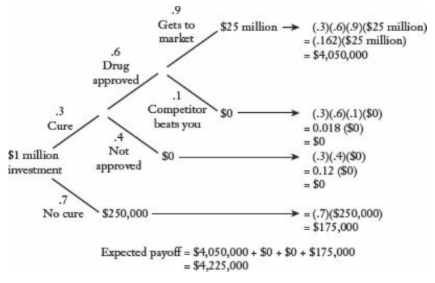
\includegraphics[width=0.7\linewidth]{images/Drug_Investment} 

}

\caption{Drug trial tree diagram (source: Wheelan)}\label{fig:wheelan-drug}
\end{figure}

This figure represents the drug approval process from investment to pay off in the form of a tree.\footnote{This is a metaphor that mathematicians actually use; the network of lines is a tree because it has no closed loops and there is one unique path to get from the beginning to any of the end-points, which are called leaf nodes.} At each branch-point of the graph, there are two possibilities: first, you may or may not develop a drug that cures a particular disease. Next, even if the drug works, it may or may not get approved. And even if it gets approved, it may or may not make it to the market. At each branch, there are also two probabilities corresponding to each path. The end-points of the branches are the leaf nodes of the tree diagram. In this particular tree, one of each forking paths is always a dead-end, or leaf. But the tree can branch in other ways.

Here are some questions to consider

\begin{enumerate}
\def\labelenumi{\arabic{enumi}.}
\tightlist
\item
  The final probabilities at each end-point are products of the probabilities along the path to get there. Why?
\item
  How do you think we estimate these branching probabilities in practice?
\end{enumerate}

\hypertarget{why-why-why-multiply-ay-ay}{%
\subsection*{Why why why multiply-ay-ay?}\label{why-why-why-multiply-ay-ay}}
\addcontentsline{toc}{subsection}{Why why why multiply-ay-ay?}

For the first question, you might reason through the probability ``math'' as follows. Say this drug investment happens in 1000 alternate universes. In 700 of them, the drug turns out to be a dud, and there is nothing more to say. But in 300 of them it is a wonder-cure. \emph{Of the 300 universes in which the drug worked,} it is not approved for use in 120 but is approved for use in 180. And so on. This winnowing-down or funneling of our imagined 1000 cases shows that you must keep applying these proportional cuts in sequence. That is, you take 0.3 of the starting amount (300/1000), and then 0.4 of that mount (120/300), which is equivalent to multiplying 1000 by 0.3 and then 0.4. Note that the language in the italicized phrase (``of the\ldots{}'') is suggestive of the language of conditional probabilities (e.g., ``given that\ldots{}''). This hints at another, perhaps more formal, description of why we multiply probabilities along the path in the tree.

To get to the endpoint, for example that ``a competitor beats you to market,'', three things need to happen. The drug must be a cure, it must be approved, and the competitor must beat you. These are three events, and the probability we need in order to compute expected value is the \emph{joint} probability of all of them. That is, P(Cure AND Approved AND Beaten) or P(C, A, B). It is tempting to invoke the rule for independent probabilities to explain why this joint probability is the product of the individual probabilities. But it would be missing an important subtlety. These events are \emph{not} independent; they are only conditionally independent. The probability of being approved is zero if the drug is not a cure. So we clearly cannot say that knowing the drug is a cure does not change our expectation of its likelihood of approval.

Rather, what is happening here is that we are multiplying conditional probabilities. And we are doing so in accordance with the definition of conditional probabilities that we saw in Chapter \ref{somefacts}. Namely, we defined the relationship between joint probabilities and conditional probabilities this way:

\begin{verbatim}
P(A and C) = P(A|C) * P(C).
\end{verbatim}

In fact, we could keep going for joint probabilities of more than two events. Suppose we added event B to the joing event \{A and C\}. Then, following above

\begin{verbatim}
P(B and A and C) = P(B|A and C) * P(A and C)
                 = P(B|A and C) * P(A|C) * P(C)
\end{verbatim}

In the second line, we used the previous result. This is sometimes written with commas instead of the word ``and.'' as,

`\texttt{P(B,\ A,\ C)\ =\ P(B\textbar{}A,\ C)\ *\ P(A\textbar{}C)\ *\ P(C).}

This unpacking of a joint probability in terms of conditional probabilities is always true, because it follows from definitions. It is only useful, however, if we know the probabilities on the right hand side. In the case of the example we started from, we do. We wanted to know P(Cure AND Approved AND Beaten). It is just

\begin{verbatim}
P(Cure AND Approved AND Beaten)  = P(Beaten | Approved, Cure) * P(Approved | Cure) * P(Cure)
                                 = (0.1) * (0.6) * (0.3)
\end{verbatim}

So this is another way to understand why we multiply the probabilities.

\hypertarget{where-do-branching-probabilities-come-from}{%
\subsection*{Where do branching probabilities come from?}\label{where-do-branching-probabilities-come-from}}
\addcontentsline{toc}{subsection}{Where do branching probabilities come from?}

In our workhorse drug-to-market investment example, we used probabilities \emph{prospectively}, that is forward-looking, to evaluate expected value. We put some probabilities in by hand. Presumably if we wanted to base these numbers on more than just our imagination, we would look for data from the past (retrospectively). We're not going to find a lot of data about cancer-curing drugs, but there have been lots of other drugs tested, approved, and/or first-to-market to treat other diseases. Specifically, we would try to find a data set that contained the following column names: Drug, Cost to develop, Success in testing, FDA Approval, First to Market, Total Sales. Or something like that. If we had such a data set, then we could actually fit a tree to it.

I'll show you how it is done in principle by making a data set that instantiates Wheelan's fictional data and then fitting it. I will make 1000 cases using Wheelan's numbers exactly, which is artificial, but it demonstrates the point. That is, my 1000 cases will have the proportions of outcomes that are dictated by the probabilities we used above. Here's one way to make the data (you can copy this code and experiment with it in your own R session).

\begin{Shaded}
\begin{Highlighting}[]
\NormalTok{wheelan\_cancer }\OtherTok{\textless{}{-}} \FunctionTok{data.frame}\NormalTok{(}
   \AttributeTok{Drug =} \FunctionTok{paste0}\NormalTok{(}\StringTok{"Drug"}\NormalTok{, }\DecValTok{1}\SpecialCharTok{:}\DecValTok{1000}\NormalTok{), }\CommentTok{\# this is just a dummy ID}
   \AttributeTok{Cure =} \FunctionTok{c}\NormalTok{(}\FunctionTok{rep}\NormalTok{(}\StringTok{"No"}\NormalTok{,}\DecValTok{700}\NormalTok{), }\FunctionTok{rep}\NormalTok{(}\StringTok{"Yes"}\NormalTok{,}\DecValTok{300}\NormalTok{)), }\CommentTok{\# 70\% of drugs will fail to cure}
   \AttributeTok{Approved =} \FunctionTok{c}\NormalTok{(}\FunctionTok{rep}\NormalTok{(}\ConstantTok{NA}\NormalTok{,}\DecValTok{700}\NormalTok{), }\FunctionTok{rep}\NormalTok{(}\StringTok{"No"}\NormalTok{,}\DecValTok{120}\NormalTok{), }\FunctionTok{rep}\NormalTok{(}\StringTok{"Yes"}\NormalTok{,}\DecValTok{180}\NormalTok{)),}
   \AttributeTok{First2Market =} \FunctionTok{c}\NormalTok{(}\FunctionTok{rep}\NormalTok{(}\ConstantTok{NA}\NormalTok{,}\DecValTok{820}\NormalTok{), }\FunctionTok{rep}\NormalTok{(}\StringTok{"No"}\NormalTok{, }\DecValTok{18}\NormalTok{), }\FunctionTok{rep}\NormalTok{(}\StringTok{"Yes"}\NormalTok{,}\DecValTok{162}\NormalTok{)),}
   \AttributeTok{Payout =} \FunctionTok{c}\NormalTok{(}\FunctionTok{rep}\NormalTok{(}\DecValTok{250000}\NormalTok{,}\DecValTok{700}\NormalTok{), }\FunctionTok{rep}\NormalTok{(}\DecValTok{0}\NormalTok{,}\DecValTok{120}\NormalTok{), }\FunctionTok{rep}\NormalTok{(}\DecValTok{0}\NormalTok{, }\DecValTok{18}\NormalTok{), }\FunctionTok{rep}\NormalTok{(}\DecValTok{25000000}\NormalTok{,}\DecValTok{162}\NormalTok{))}
\NormalTok{)}
\end{Highlighting}
\end{Shaded}

Notice that I had to use the missing value ``NA'' in the table that I made. If the drug does not cure the disease, the the approval status is neither Yes nor No.~It never gets to that stage. So the approval value for those drugs is missing. The data has 1000 rows, many of which are identical. I will show the rows where things change. In between we have a lot of replicas, i.e., drugs with the same exact story.

\begin{table}[!h]

\caption{\label{tab:unnamed-chunk-26}A fake drug development dataset}
\centering
\begin{tabular}[t]{llllr}
\toprule
Drug & Cure & Approved & First2Market & Payout\\
\midrule
Drug1 & No & NA & NA & 250000\\
Drug700 & No & NA & NA & 250000\\
Drug701 & Yes & No & NA & 0\\
Drug820 & Yes & No & NA & 0\\
Drug821 & Yes & Yes & No & 0\\
\addlinespace
Drug838 & Yes & Yes & No & 0\\
Drug839 & Yes & Yes & Yes & 25000000\\
Drug1000 & Yes & Yes & Yes & 25000000\\
\bottomrule
\end{tabular}
\end{table}

Now this last part is a bit of black magic, since I have not said anything about how one ``fits'' a tree, also known as a recursive partition, to data. But here it is. It can be done using a R package called \texttt{rpart} (for recursive partitioning).

\begin{Shaded}
\begin{Highlighting}[]
\FunctionTok{library}\NormalTok{(rpart)}
\FunctionTok{library}\NormalTok{(rpart.plot)}
\NormalTok{wheelan\_tree }\OtherTok{\textless{}{-}} \FunctionTok{rpart}\NormalTok{(}
\NormalTok{  Payout }\SpecialCharTok{\textasciitilde{}}\NormalTok{ Cure }\SpecialCharTok{+}\NormalTok{ Approved }\SpecialCharTok{+}\NormalTok{ First2Market, }
  \AttributeTok{data =}\NormalTok{ wheelan\_cancer, }
  \AttributeTok{method =} \StringTok{"anova"}
\NormalTok{)}
\end{Highlighting}
\end{Shaded}

Ta-da! Don't believe me? Here is the tree.

\begin{Shaded}
\begin{Highlighting}[]
\FunctionTok{rpart.plot}\NormalTok{(wheelan\_tree, }\AttributeTok{type =} \DecValTok{5}\NormalTok{, }\AttributeTok{digits=}\DecValTok{3}\NormalTok{)}
\end{Highlighting}
\end{Shaded}

\begin{center}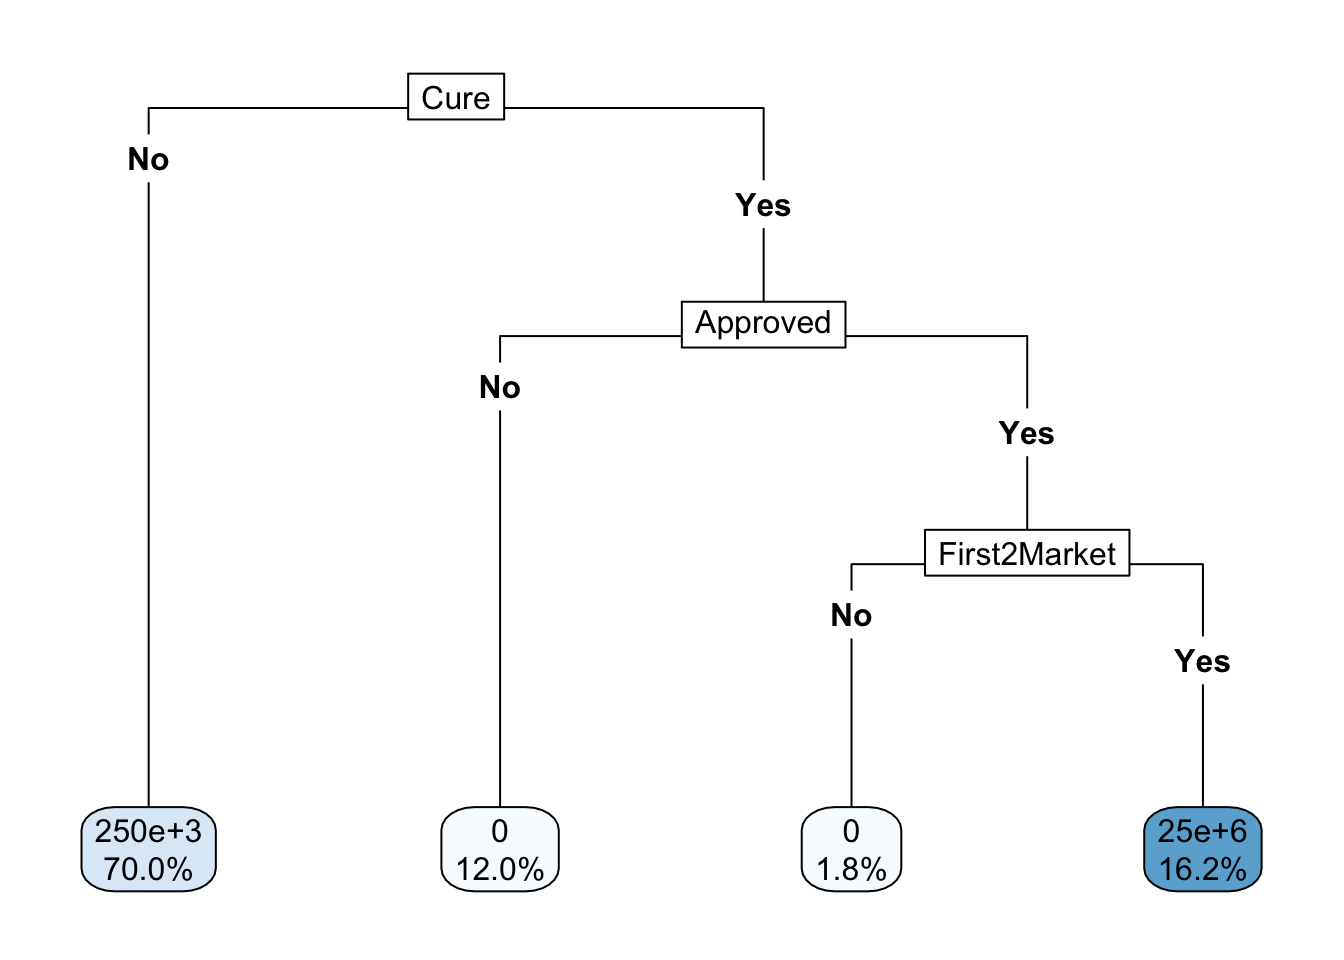
\includegraphics[width=0.9\linewidth,]{carpedatum_files/figure-latex/unnamed-chunk-28-1} \end{center}

The leaf nodes at the bottom (rpart makes top-down trees) show the payout using scientific notation. I don't know how to suppress that. You can see both the payout and the probability of the payout.

Hopefully you can see that expected value is quite general. You could use this kind of thinking, for example, to estimate your future income based on decisions you can make about your life. Suppose you major in acting AND you get discovered on the streets of Greenwich Village AND your indie debut film leads to superstardom as the next Marvel superhero! But what if your indie debut never gets off the ground? What if you had majored in accounting instead? Maybe you went to work for a big investment bank, or perhaps it was just a small tax office. If you assign numbers to the scenario above, you can calculate the expected value of your college major in terms of earnings.

Of course, there are no guarantees, only probabilities.

\hypertarget{is-the-system-fair}{%
\chapter*{Is the System Fair?}\label{is-the-system-fair}}
\addcontentsline{toc}{chapter}{Is the System Fair?}

At this point in the course, you've seen how variance in outcomes can be understood in terms of random, or noisy, statistical processes. If you bet on red at the roulette table five times in a row, and if you lose five times, that doesn't mean the roulette wheel isn't fair. That just could be bad luck (for you; possibly good luck for someone else who betted on black). Of course, the casino odds are stacked against you in the long run, since the casino always has an edge. For example, bets on red or black have even odds, but there are two out of 38 possible roulette outcomes in which neither black nor red will win. Now, in principle everyone knows that this is how casinos work and stay in business. So if you end up losing more often than you win in a casino, you can only blame yourself.

Sometimes, though, outcomes are distributed in a certain way that causes us to question whether everything is indeed working \emph{as it is supposed to be}, according to the rules of probability and some inner sense of fairness. In particular, when outcomes differ for some group or groups of people, we sometimes worry if the system is fair. You may have heard people say, the system isn't fair. Well, sometimes it isn't. And we might be able to identify a problem and even fix it. For this to work, though, we need to understand what outcomes are fair outcomes, and this turns out to be a complicated issue! At the root of this inquiry is understanding and explaining differences between groups.

\hypertarget{differences-in-athletics}{%
\chapter{Differences in athletics}\label{differences-in-athletics}}

\hypertarget{are-professional-basketball-players-taller}{%
\section*{Are professional basketball players taller?}\label{are-professional-basketball-players-taller}}
\addcontentsline{toc}{section}{Are professional basketball players taller?}

Let's start with an example to refresh your memory about sampling and differences. We'll walk through this example very naively on purpose. Suppose we take 100 NBA basketball players as a sample (of all basketball players) and 100 NYU students as another sample (of NYU students), and now we look at the distribution of heights in each of our samples. We'll consider male students, since the NBA players are also males. Actually, I don't have any data on NYU student heights. So we'll just consider all adult males. Conveniently, the \texttt{openintro} R package has a data set called male.heights and another data set called \texttt{nba.heights}. You can load them as follows

\begin{Shaded}
\begin{Highlighting}[]
\FunctionTok{library}\NormalTok{(openintro)}
\FunctionTok{data}\NormalTok{(}\StringTok{"male\_heights"}\NormalTok{)}
\FunctionTok{data}\NormalTok{(}\StringTok{"nba\_heights"}\NormalTok{)}
\end{Highlighting}
\end{Shaded}

And then you can inspect them. For example, one of the first things I will do with a data set is ask how big it is (how many rows and columns) and then look at the first few rows.

\begin{Shaded}
\begin{Highlighting}[]
\FunctionTok{dim}\NormalTok{(male\_heights)}
\end{Highlighting}
\end{Shaded}

\begin{verbatim}
## [1] 100   1
\end{verbatim}

\begin{Shaded}
\begin{Highlighting}[]
\FunctionTok{head}\NormalTok{(male\_heights)}
\end{Highlighting}
\end{Shaded}

\begin{verbatim}
## # A tibble: 6 x 1
##   heights
##     <int>
## 1      71
## 2      67
## 3      69
## 4      70
## 5      68
## 6      63
\end{verbatim}

The \texttt{male\_heights} data table has 100 rows and a single column called ``heights.'' The nba.heights data set is a little different.

\begin{Shaded}
\begin{Highlighting}[]
\FunctionTok{dim}\NormalTok{(nba\_heights)}
\end{Highlighting}
\end{Shaded}

\begin{verbatim}
## [1] 435   4
\end{verbatim}

\begin{Shaded}
\begin{Highlighting}[]
\FunctionTok{head}\NormalTok{(nba\_heights)}
\end{Highlighting}
\end{Shaded}

\begin{verbatim}
## # A tibble: 6 x 4
##   last_name first_name h_meters  h_in
##   <chr>     <chr>         <dbl> <int>
## 1 Acker     Alex           1.96    77
## 2 Adams     Hassan         1.93    76
## 3 Afflalo   Arron          1.96    77
## 4 Ager      Maurice        1.96    77
## 5 Ajinca    Alexis         2.13    84
## 6 Aldridge  LaMarcus       2.11    83
\end{verbatim}

Notice that there are 435 NBA players from the 2008-2009 season here. We have their first and last names as well as their heights in units of meters and also inches. I'd like to make a comparison between similarly sized samples. So I will just take a subsample of 100 NBA players. I can do this easily using the \texttt{sample()} function.

\begin{Shaded}
\begin{Highlighting}[]
\CommentTok{\# sample 100 values at random from the nba heights in inches}
\NormalTok{nbaHeights }\OtherTok{\textless{}{-}} \FunctionTok{sample}\NormalTok{(nba\_heights}\SpecialCharTok{$}\NormalTok{h\_in, }\DecValTok{100}\NormalTok{) }
\CommentTok{\# rename the male height to match}
\NormalTok{maleHeights }\OtherTok{\textless{}{-}}\NormalTok{ male\_heights}\SpecialCharTok{$}\NormalTok{heights}
\end{Highlighting}
\end{Shaded}

Note that because I did not use a \texttt{set.seed} in the code above, I have no idea which 100 NBA players I got. In fact, every time I (or you) run this, I (or you) will get a different sample! Finally, I would like to compare the \emph{distributions} of heights for these two samples. For which our old friend the histogram is just what the doctor ordered.

\begin{Shaded}
\begin{Highlighting}[]
\CommentTok{\# defining some colors and bin{-}breaks to standardize my plots}
\NormalTok{malescol }\OtherTok{\textless{}{-}} \FunctionTok{rgb}\NormalTok{(}\FloatTok{0.8}\NormalTok{,}\FloatTok{0.2}\NormalTok{,}\DecValTok{0}\NormalTok{,}\FloatTok{0.2}\NormalTok{)}
\NormalTok{nbacol }\OtherTok{\textless{}{-}} \FunctionTok{rgb}\NormalTok{(}\DecValTok{0}\NormalTok{,}\FloatTok{0.3}\NormalTok{,}\FloatTok{0.8}\NormalTok{,}\FloatTok{0.2}\NormalTok{)}
\NormalTok{mybreaks }\OtherTok{\textless{}{-}} \FunctionTok{seq}\NormalTok{(}\DecValTok{54}\NormalTok{,}\DecValTok{90}\NormalTok{,}\DecValTok{3}\NormalTok{)}

\CommentTok{\# plot a histogram showing both height distributions, separately}
\FunctionTok{hist}\NormalTok{(maleHeights, }\AttributeTok{col=}\NormalTok{malescol, }\AttributeTok{breaks=}\NormalTok{mybreaks, }
          \AttributeTok{main=}\StringTok{"Heights of males"}\NormalTok{, }\AttributeTok{xlab=}\StringTok{"Height (inches)"}\NormalTok{)}
\end{Highlighting}
\end{Shaded}

\begin{center}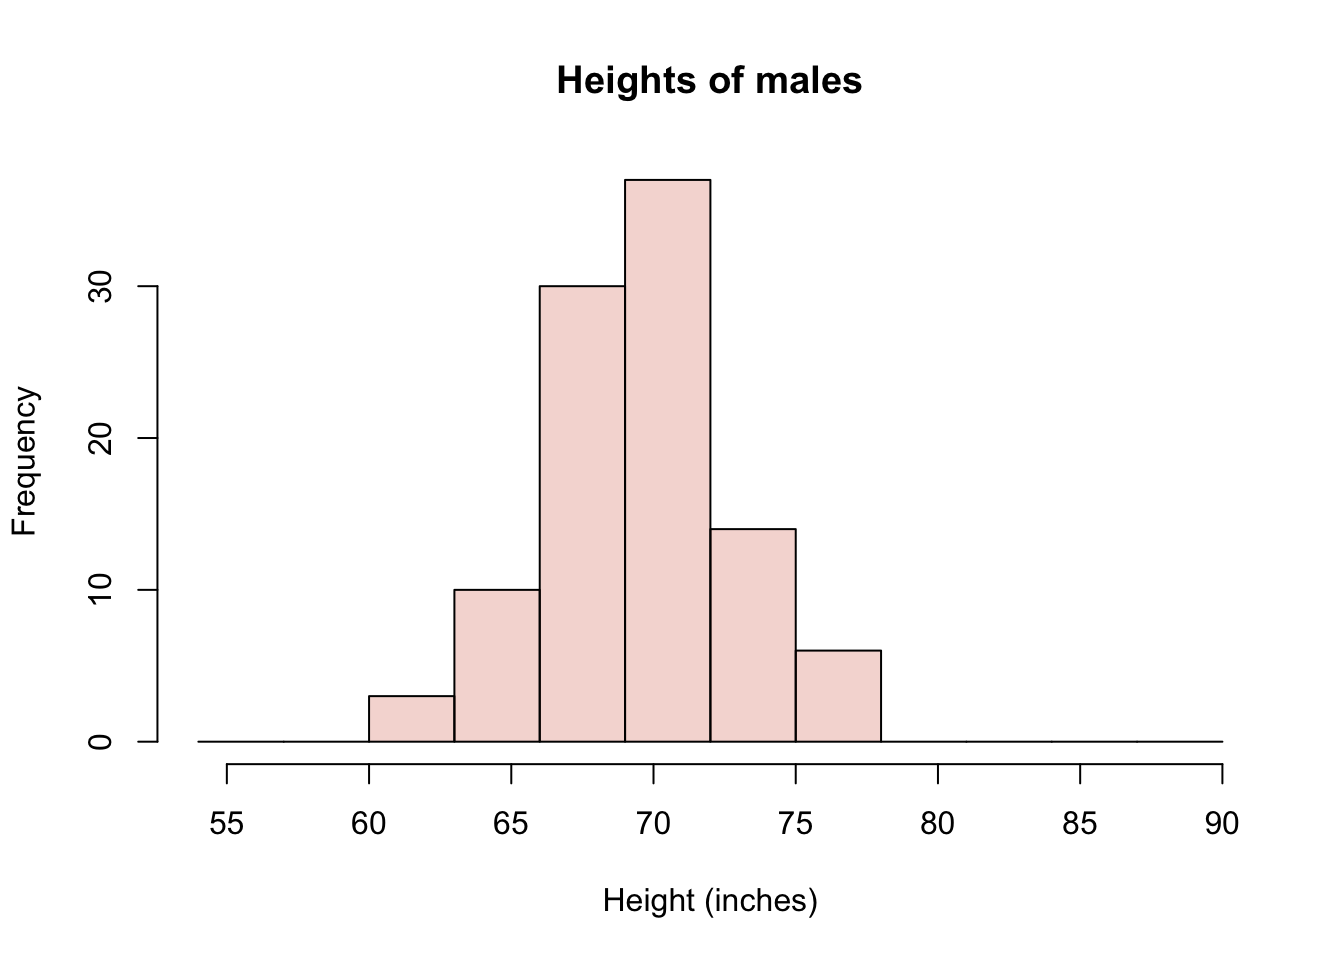
\includegraphics[width=0.9\linewidth]{carpedatum_files/figure-latex/unnamed-chunk-33-1} \end{center}

\begin{Shaded}
\begin{Highlighting}[]
\FunctionTok{hist}\NormalTok{(nbaHeights, }\AttributeTok{col=}\NormalTok{nbacol, }\AttributeTok{breaks=}\NormalTok{mybreaks, }
     \AttributeTok{main=}\StringTok{"Heights of NBA players"}\NormalTok{, }\AttributeTok{xlab=}\StringTok{"Height (inches)"}\NormalTok{)}
\end{Highlighting}
\end{Shaded}

\begin{center}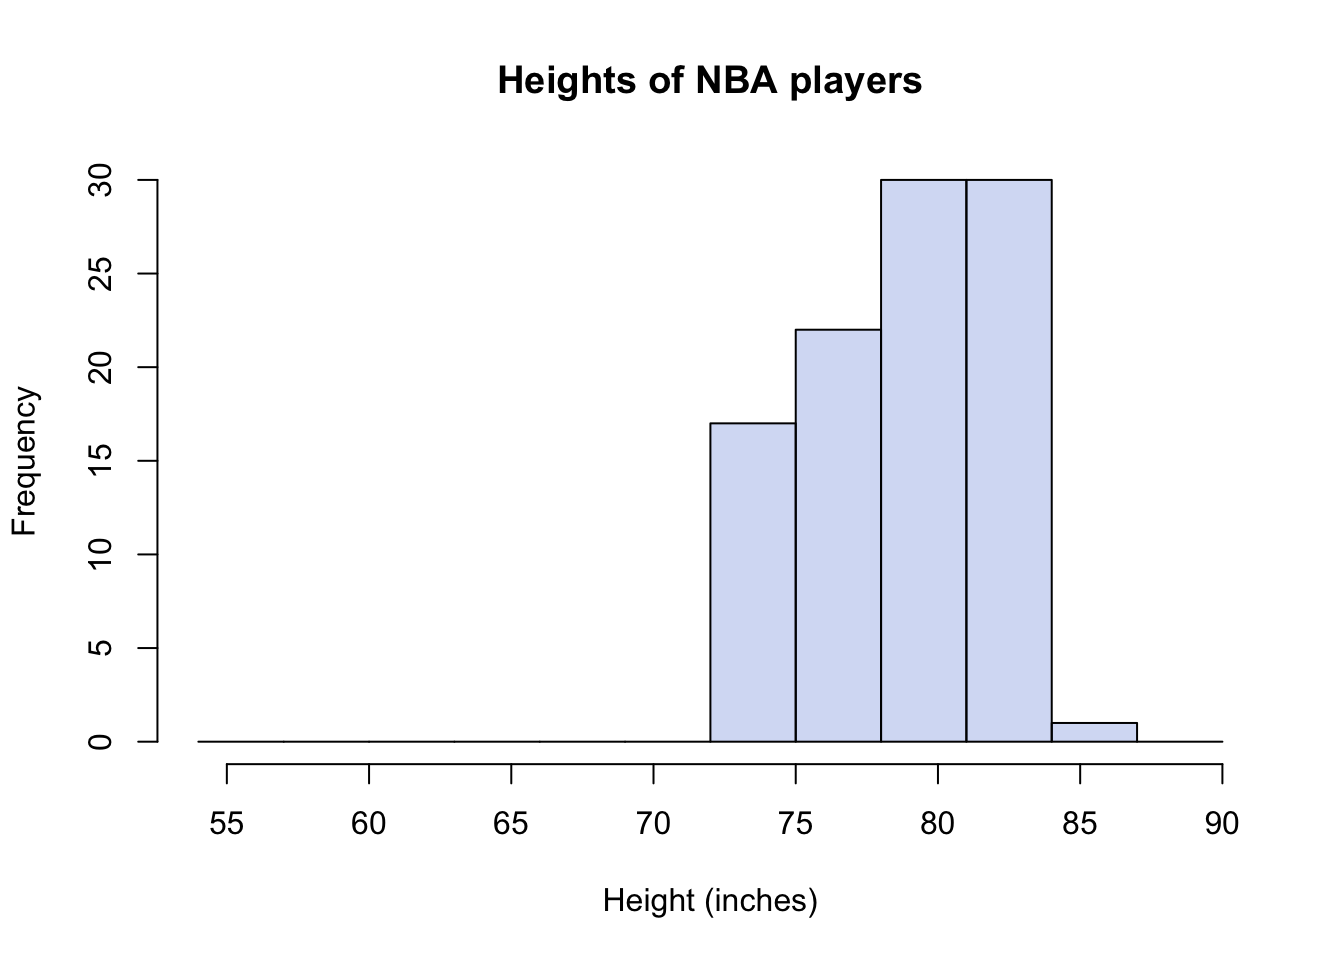
\includegraphics[width=0.9\linewidth]{carpedatum_files/figure-latex/unnamed-chunk-33-2} \end{center}

\begin{Shaded}
\begin{Highlighting}[]
\CommentTok{\# plot a histogram showing both height distributions, together (add=T)}
\FunctionTok{hist}\NormalTok{(maleHeights, }\AttributeTok{col=}\NormalTok{malescol, }\AttributeTok{breaks=}\NormalTok{mybreaks, }
          \AttributeTok{main=}\StringTok{""}\NormalTok{, }\AttributeTok{xlab=}\StringTok{"Height (inches)"}\NormalTok{)}
\FunctionTok{hist}\NormalTok{(nbaHeights, }\AttributeTok{col=}\NormalTok{nbacol, }\AttributeTok{breaks=}\NormalTok{mybreaks, }\AttributeTok{add=}\NormalTok{T)}
\FunctionTok{legend}\NormalTok{(}\StringTok{"topleft"}\NormalTok{, }\FunctionTok{c}\NormalTok{(}\StringTok{"non{-}NBA"}\NormalTok{, }\StringTok{"NBA"}\NormalTok{), }\AttributeTok{fill =} \FunctionTok{c}\NormalTok{(malescol, nbacol))}
\end{Highlighting}
\end{Shaded}

\begin{figure}

{\centering 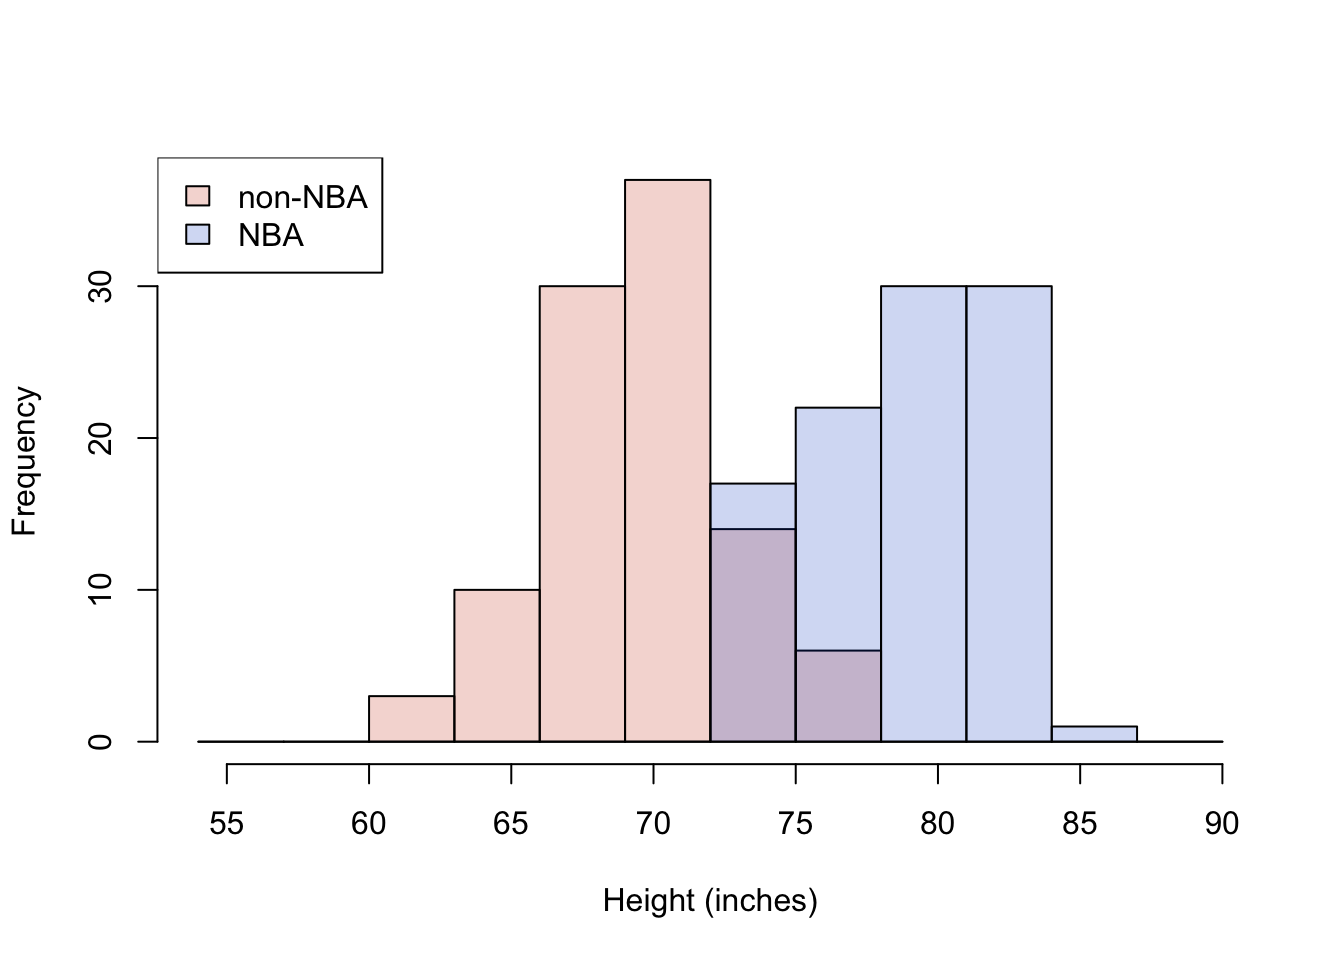
\includegraphics[width=0.9\linewidth]{carpedatum_files/figure-latex/compareheights-1} 

}

\caption{Histogram of NBA and non-NBA male heights on one plot using transparent colors}\label{fig:compareheights}
\end{figure}

I have shown three histograms, one with only the males dataset, one with only the NBA data set, and one showing both groups at the same time. I've made the colors in R slightly transparent, so that both distributions are visible at the same time. But it is very important to recognize that in Figure \ref{fig:compareheights}, we are seeing an overlap region of two distributions, \emph{not} three distributions shown with ``stacked bars.'' You sometimes see stacked barplots, where the height of the bar is the total count, and the colors represent contributions to the total from different groups. For example, units sold in the USA and units sold abroad = total units sold. Here, you don't see the total. You would have to estimate it by mentally adding up the \emph{full heights} of each bar. So, for example, the total number (out of 200) of males in the height range of 72-75 inches would be 14 from the males data set plus 17 from the NBA dataset.

I doubt any of you reading this are surprised to see that there is a big difference in these distributions; that NBA players are, on average, 9 or 10 inches taller than the (average) males. For the particular subsample I've drawn, the difference happens to be exactly 9.5 inches.

Now that you are somewhat conversant with sampling variation, you might wonder: what are the chances of a difference in sample heights like this occuring by chance? After all, if we had a large group of males to begin with, and we sampled from them two different times, we would not expect the averages of the two samples to be identical. We will probably get a taller sample and a shorter sample, right? But how much taller?

You can actually simulate and/or calculate an answer to these questions. Which of the following would you need to know in order to estimate the chances of a large difference in height occuring by chance?

\begin{enumerate}
\def\labelenumi{\arabic{enumi}.}
\tightlist
\item
  Group sample means (averages)
\item
  Group sample variances (a measure of spread)
\item
  Sample size of groups
\end{enumerate}

\begin{enumerate}
\def\labelenumi{\Alph{enumi})}
\tightlist
\item
  1 \& 2 only
\item
  2 \& 3 only
\item
  1 \& 3 only
\item
  1, 2, \& 3
\end{enumerate}

Answer.\footnote{The answer is D. Here's why you need each quantity. \textbf{Sample means.} Clearly, if the sample means are very close, you are more likely to accept the possibility that the difference occurred by chance than if they are very different, so sample means are necessary. On the heels of that, the notion of ``close'' values of the means is itself dependent on the range of values we expect (i.e., on the \textbf{variance} or spread). Two buildings are close in height if one is 271 ft tall and another is 274 ft tall. But a difference of 3 feet among human beings is enormous. It's enormous \emph{relative} to the standard deviation, which for adult human beings is about 4 inches. The standard deviation for building heights is over 200 ft if we include skyscrapers. Finally, the \textbf{sample size.} The law of large numbers tells us that the sample mean gets closer to the population mean as the sample size increases. However, when the sample size is small, we will have more sampling variance. Intuitively, we can think about it this way: Let's suppose the distributions are different but not so different that they don't overlap. If we sample only two people from each population, we may get two tall people by chance from one (or short ones from the other) in such a way that the means are close by chance. But if we have small differences in means with large samples (say, 1000), then we believe that the means are, in fact, close or even equal.}

We can go to the National Center for Health Statistics website to retrieve a larger census of male heights. (You can find Body Measures in the National Health and Nutrition Examination Survey conducted every two years.) Conveniently (again) someone has even made an R package to save you the time (\texttt{NHANES}). The data set includes females as well as children, so I will filter those out. Here is a distribution of roughly 3600 males.

\begin{Shaded}
\begin{Highlighting}[]
\FunctionTok{library}\NormalTok{(NHANES) }\CommentTok{\#}
\FunctionTok{library}\NormalTok{(dplyr)}

\NormalTok{lotsoheights }\OtherTok{\textless{}{-}}\NormalTok{ NHANES }\SpecialCharTok{\%\textgreater{}\%} \FunctionTok{filter}\NormalTok{(Gender }\SpecialCharTok{==} \StringTok{"male"} \SpecialCharTok{\&}\NormalTok{ Age }\SpecialCharTok{\textgreater{}} \DecValTok{18}\NormalTok{) }\SpecialCharTok{\%\textgreater{}\%} 
                                \FunctionTok{select}\NormalTok{(Height) }\SpecialCharTok{\%\textgreater{}\%} \FunctionTok{unlist}\NormalTok{() }\SpecialCharTok{\%\textgreater{}\%} \FunctionTok{na.omit}\NormalTok{()}
\CommentTok{\# convert cm to in}
\NormalTok{lotsoheights }\OtherTok{\textless{}{-}} \FunctionTok{as.numeric}\NormalTok{(lotsoheights) }\SpecialCharTok{/} \FloatTok{2.54}

\CommentTok{\# plot as before}
\FunctionTok{hist}\NormalTok{(lotsoheights, }\AttributeTok{col=}\NormalTok{malescol, }\AttributeTok{breaks=}\NormalTok{mybreaks, }
          \AttributeTok{main=}\StringTok{"Heights of 3600 males"}\NormalTok{, }\AttributeTok{xlab=}\StringTok{"Height (inches)"}\NormalTok{)}
\end{Highlighting}
\end{Shaded}

\begin{center}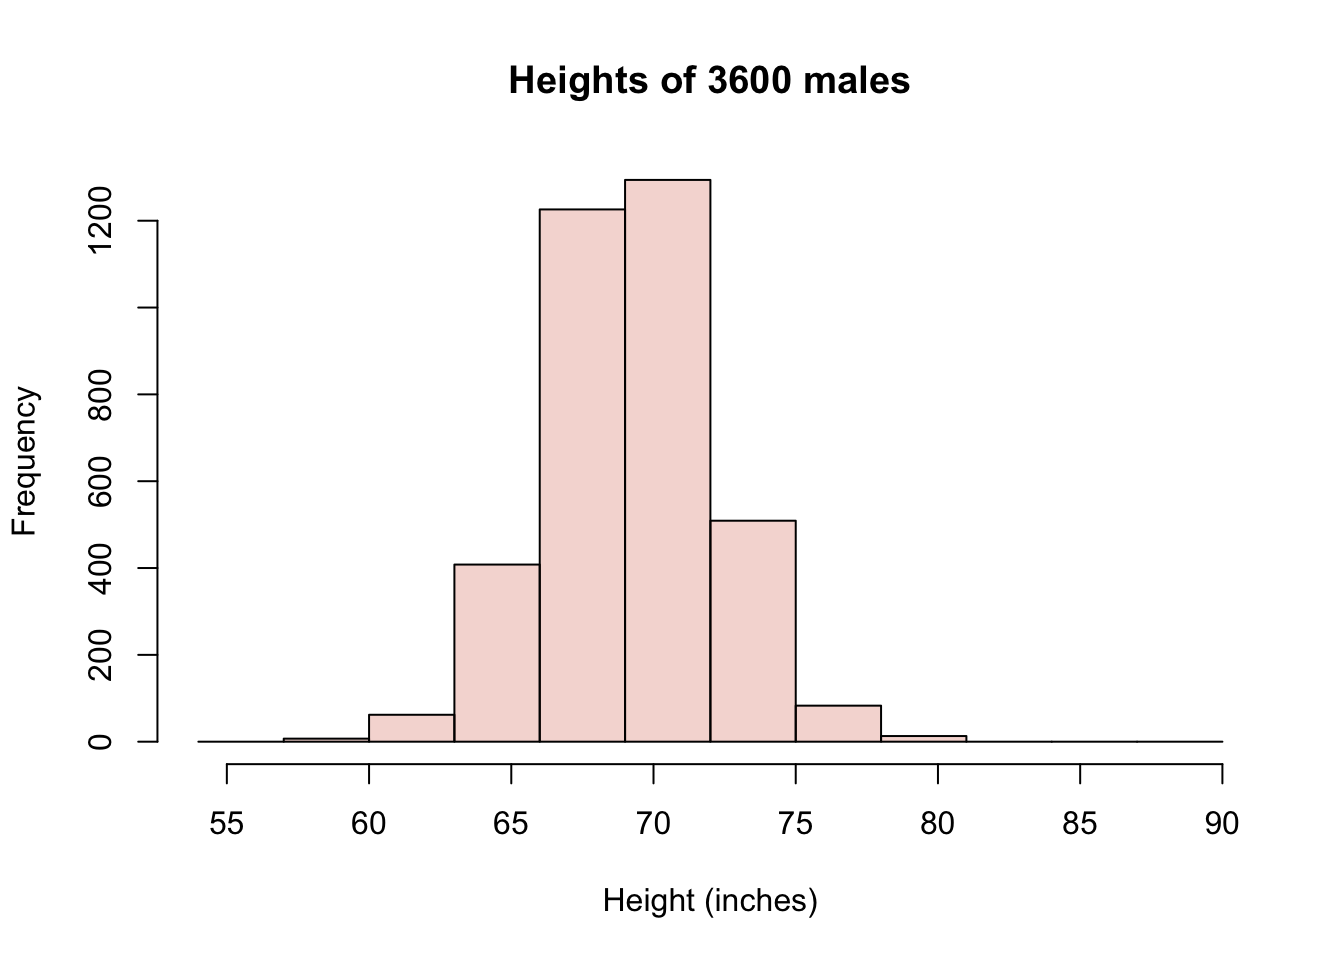
\includegraphics[width=0.9\linewidth]{carpedatum_files/figure-latex/unnamed-chunk-35-1} \end{center}

Now consider a process of sub-sampling from this larger sample repeatedly. That is, we take two samples of 100 and compare the difference in the sample averages. Let's say we do it 1000 times. How often do we see differences as extreme as 9 inches? Mind you, we have no idea which of our two samples will turn out taller, so we'll need to look for differences with magnitude (or absolute value) greater than 9. Because the difference could be 9.5 or -9.5 depending on the order of subtraction. Here goes:

\begin{Shaded}
\begin{Highlighting}[]
\NormalTok{numSamples }\OtherTok{\textless{}{-}} \DecValTok{1000}
\NormalTok{sampleSize }\OtherTok{\textless{}{-}} \DecValTok{100}
\NormalTok{differences\_in\_means }\OtherTok{\textless{}{-}} \FunctionTok{c}\NormalTok{()}
\ControlFlowTok{for}\NormalTok{ (i }\ControlFlowTok{in} \DecValTok{1}\SpecialCharTok{:}\NormalTok{numSamples) \{}
\NormalTok{  sample1 }\OtherTok{\textless{}{-}} \FunctionTok{sample}\NormalTok{(lotsoheights, sampleSize)}
\NormalTok{  sample2 }\OtherTok{\textless{}{-}} \FunctionTok{sample}\NormalTok{(lotsoheights, sampleSize)}
\NormalTok{  differences\_in\_means }\OtherTok{\textless{}{-}} \FunctionTok{c}\NormalTok{(differences\_in\_means, }\FunctionTok{mean}\NormalTok{(sample1) }\SpecialCharTok{{-}} \FunctionTok{mean}\NormalTok{(sample2))}
\NormalTok{\}}

\FunctionTok{hist}\NormalTok{(differences\_in\_means)}
\end{Highlighting}
\end{Shaded}

\begin{center}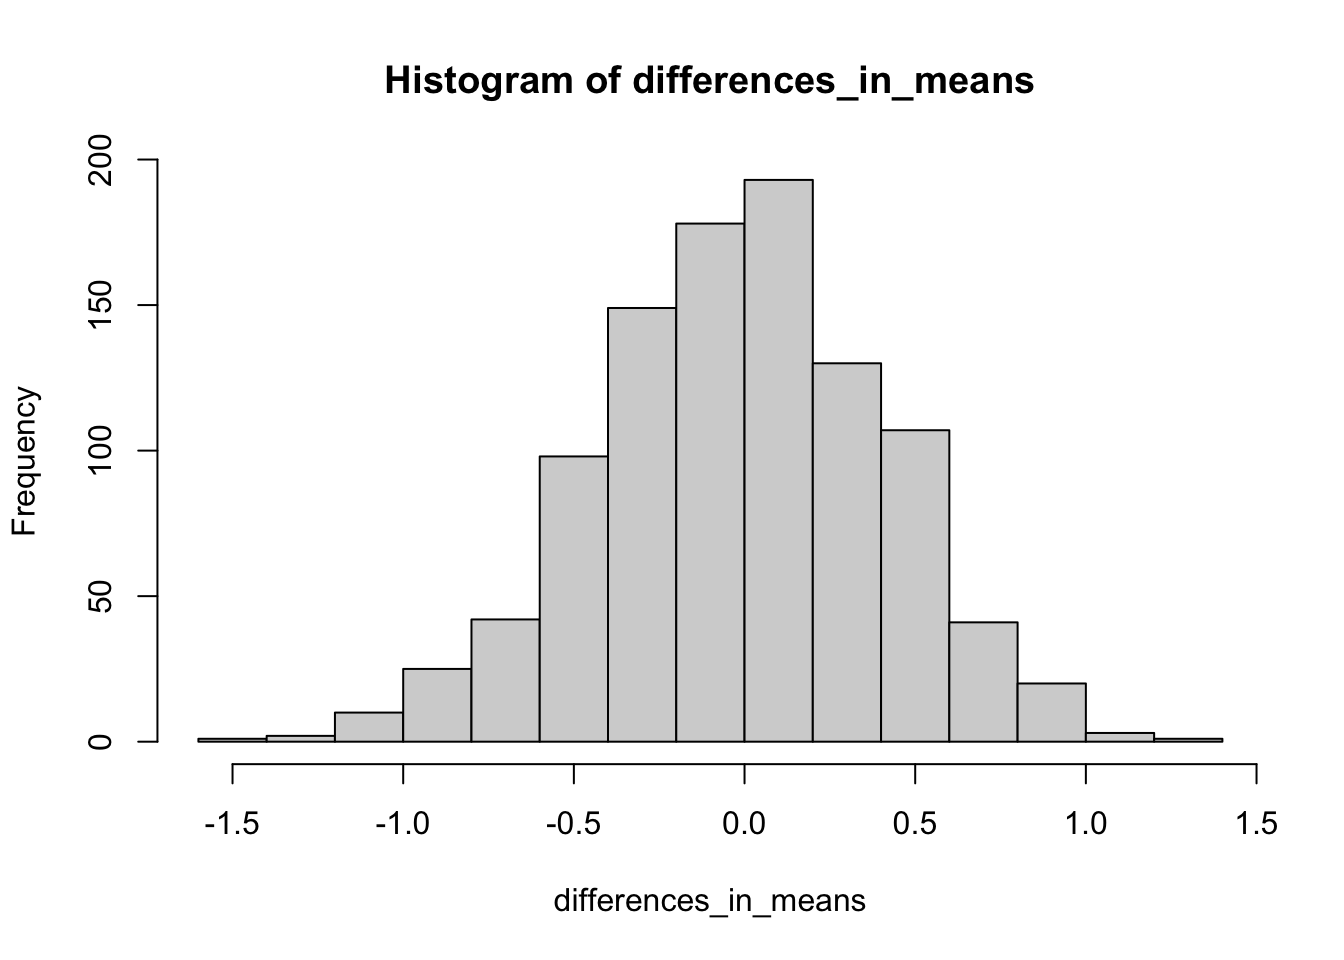
\includegraphics[width=0.9\linewidth]{carpedatum_files/figure-latex/unnamed-chunk-36-1} \end{center}

You'll notice that in 1000 experiments, we never observed a difference in mean heights between our two samples of even 2 inches, let alone 9 inches. Here is how you would know for sure

\begin{Shaded}
\begin{Highlighting}[]
\CommentTok{\# declare a threshold difference of interest}
\NormalTok{thresholdDiff }\OtherTok{\textless{}{-}} \DecValTok{9}
\CommentTok{\# compute percentage of events outside of this threshold}
\NormalTok{numExtreme }\OtherTok{\textless{}{-}} \FunctionTok{length}\NormalTok{(}\FunctionTok{which}\NormalTok{(}\FunctionTok{abs}\NormalTok{(differences\_in\_means) }\SpecialCharTok{\textgreater{}}\NormalTok{ thresholdDiff))}
\NormalTok{percentExtreme }\OtherTok{\textless{}{-}}\NormalTok{ numExtreme}\SpecialCharTok{/}\NormalTok{numSamples }\SpecialCharTok{*} \DecValTok{100}
\FunctionTok{paste0}\NormalTok{(percentExtreme,}\StringTok{"\%"}\NormalTok{)}
\end{Highlighting}
\end{Shaded}

\begin{verbatim}
## [1] "0%"
\end{verbatim}

In short, it seems highly implausible that this difference would occur by chance.

\begin{quote}
Exercise: modify the code to use samples of 10 instead of 100. Do you observe bigger differences? And if so, are they big enough to explain the NBA difference?
\end{quote}

\begin{quote}
Exercise: Experiment with changing the threshold difference. Using the original sample size of 100, how often are differences greater than 1 inch? Where should the threshold be set so that a difference \emph{at least as large as this threshold} is expected to occur roughly 25\% of the time?
\end{quote}

\hypertarget{none-of-this-is-surprising}{%
\subsection*{None of this is surprising}\label{none-of-this-is-surprising}}
\addcontentsline{toc}{subsection}{None of this is surprising}

Okay, so suppose we accept that NBA players are systematically taller. Could it be that the NBA makes people taller? Perhaps there is special practice or vitamin supplement that NBA players use that causes them to grow 9-10 inches? Well, we could rule this out if, for example, we examined the heights of NBA players just BEFORE they became NBA players. If we did that, we would see that they were already tall.

Another possibility, then, is that NBA players are selected for being tall. The question we might now ask, though, is: is that fair? We're saying that short people have a low likelihood of being hired as NBA players. (Note that we're not suggesting that being tall is \emph{sufficient} to become an NBA player, but it does seem to be \emph{necessary}). What do you think?

Which of these statements do you most agree with?

\begin{enumerate}
\def\labelenumi{\arabic{enumi}.}
\tightlist
\item
  It is not fair; everyone should have an equal chance to play in the NBA
\item
  It is not fair; shorter people, who are exceptionally talented in basketball, should have an equal chance to play in the NBA
\item
  It is fair; tall players perform better because their height provides an advantage in the game of basketball
\item
  It is fair; tall players look better on the court than short players, and the NBA has to sell tickets.
\item
  It is neither fair nor unfair; it just is.
\end{enumerate}

It may be possible to defend different answers to this particular question of fairness, but most of us can agree that professional sports are, by design, selective on performance. In a game like basketball, height provides an advantage which, along with athleticism (strength, speed, stamina, etc.), makes a player perform better.

In summary, we have observed a difference between groups. NBA players are taller than non-NBA players. This difference does not appear to be consistent with random chance. Indeed, we probably knew enough about basketball to explain the difference in terms of selection for competitive advantage. But, importantly, it is up to us to decide whether selecting players for competitive advantage---even if it means that we effectively discriminate against short athletes---is fair.

\hypertarget{surprising-differences}{%
\section*{Surprising differences}\label{surprising-differences}}
\addcontentsline{toc}{section}{Surprising differences}

So professional basketball players are more likely to be tall. What if I told you that professional hockey players are more likely to be\ldots.born in the first three months of the calendar year. What? Yes, you heard that right. See Figure \ref{fig:hockey-fig} (Full paper: \url{https://journals.plos.org/plosone/article?id=10.1371/journal.pone.0057753}
).



\begin{figure}

{\centering 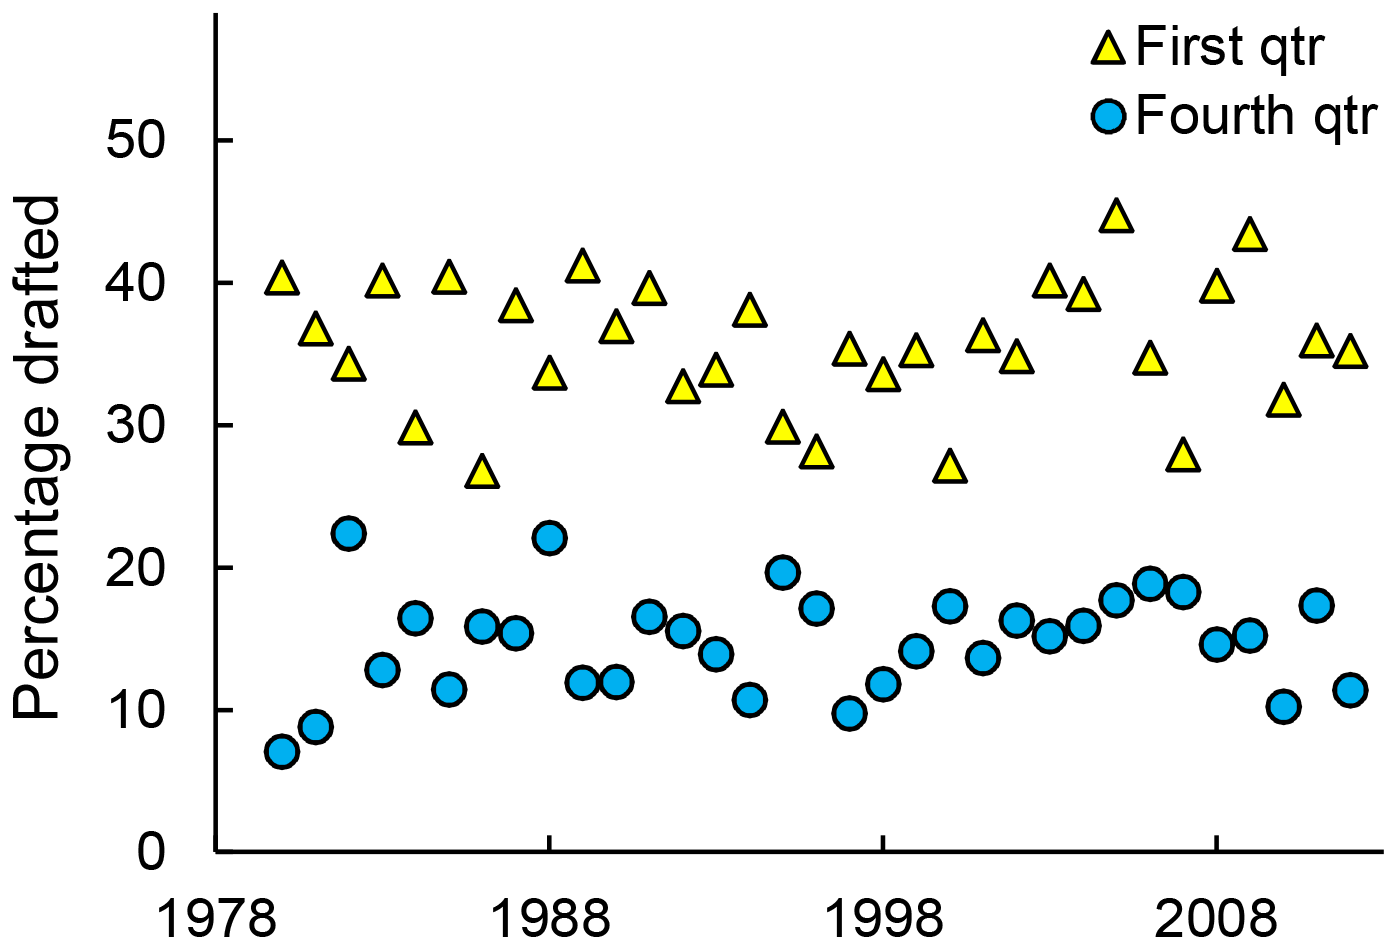
\includegraphics[width=0.7\linewidth]{images/hockeybirths} 

}

\caption{Percentage of NHL draftees born in the first or fourth quarter over time. Blue circles indicate first quarter; yellow triangles indicate fourth quarter. Source: \href{https://journals.plos.org/plosone/article?id=10.1371/journal.pone.0057753}{Born at the Wrong Time: Selection Bias in the NHL Draft}}\label{fig:hockey-fig}
\end{figure}

Okay, let's work through this idea similarly to the way we did when sampling from the NBA. That is, let us first consider the possibility that these differences are a result of sampling without systematic bias. As before, we need a baseline for comparison. For NBA heights, we needed to compare the distribution to non-NBA males. For hockey birth-months, we need a sense of birth-month distribution in the general population. I won't bother distinguishing male and female births, because I don't have any reason to believe that these occur differently month-by-month.

From this CDC source (\url{https://www.cdc.gov/nchs/fastats/births.htm}), I have produced a table of births by month in the United States from 2017.

\begin{table}[!h]

\caption{\label{tab:birthmonth-table}Births by month (USA, 2017)}
\centering
\begin{tabular}[t]{lr}
\toprule
month & count\\
\midrule
January & 313786\\
February & 289054\\
March & 319625\\
April & 300116\\
May & 322456\\
\addlinespace
June & 323920\\
July & 334924\\
August & 352151\\
September & 337175\\
October & 329869\\
\addlinespace
November & 316511\\
December & 315913\\
\bottomrule
\end{tabular}
\end{table}

Let's concentrate on the number of births and, in particular, on the first four months of the year, January, Feb, March, and April.

What do you think is the most plausible explanation for the variation in the the number of births in each of these four months?

\begin{enumerate}
\def\labelenumi{\alph{enumi}.}
\tightlist
\item
  There is chance variation is any random process, such as childbirth
\item
  Odd numbered months are more likely to have higher birth numbers
\item
  Births are likely to go up and down in month-long cycles
\item
  The number of days in each of the first four months of 2017 (not a leap year) is 31, 28, 31, 30
\end{enumerate}

Consider option (a). While the statement itself is true, the size of the variation between these months is much too large to be explained by chance alone. Sample size is key here!

If January and February were each equally likely, up to random chance, and we observed only 600 births in total instead of 600,000, then the chance of observing 313 or more births in one month or the other is actually about 27\%. That is, there's about a 13.5\% chance of January having more than 313 births and a 13.5\% chance of it having fewer than 287 births (the rest of the 600 going to February). However, even if we just up the sample to 6000, the chance of observing more than 3130 births in one month or the other goes down to about 0.05\%, while for 600,000 births, the chances of a discrepancy this large is a number so small it has no meaningful interpretation. So, in short, chance alone can't explain it.

No, you probably guessed that the length of each month explains most of this effect. But not ALL of it. If every day of the year were equally likely, we can estimate the number of expected births per day as \texttt{3855500/365\ =\ 10563}. How many births would we expect in a month that had 30 days? Well, for months with 31 days, we would expect \texttt{31*10563\ =\ 327453} births (rounding), for months with 28 days, 295764. Notice that the difference is large. Notice also, though, that it is \emph{larger} than the observed difference, and that observed monthly birth counts in January and February are both actually lower than expected. That must mean that some other months of the year get more births. And indeed this is true. Just look at July-October.

Having examined the data at the month level, we can also combine three months into quarters. Here is the quarterly count, as well as the proportion (each quarterly count divided by total).

\begin{table}[!h]

\caption{\label{tab:birthquarter}Births by quarter (USA, 2017)}
\centering
\begin{tabular}[t]{lrr}
\toprule
  & count & proportion\\
\midrule
Q1 & 922465 & 0.239\\
Q2 & 946492 & 0.245\\
Q3 & 1024250 & 0.266\\
Q4 & 962293 & 0.250\\
\bottomrule
\end{tabular}
\end{table}

Looking at this, we can see plainly that there are more births in the third quarter of the year (July-Sep) than in the first quarter (Jan-Mar). The proportions in Table \ref{tab:birthquarter} are what we would expect to see in any collection of people (e.g., professional hockey players) \emph{if they were not systematically selected for birth month}.

\hypertarget{aside-sampling-with-more-than-two-groups}{%
\subsubsection*{Aside: Sampling with more than two groups}\label{aside-sampling-with-more-than-two-groups}}
\addcontentsline{toc}{subsubsection}{Aside: Sampling with more than two groups}

Previously in this course, for example with two-types-of-people questions and with beer taste-tests, we looked at how to simulate dichotomous outcomes. We used the \texttt{sample()} function in R repeatedly, or we took advantage of the binomial distribution. The function \texttt{rbinom()} can be used to simulate many beer taste-tests, for example, and the function \texttt{dbinom()} can be used to compute the proportion of certain outcomes. Suppose we wanted to simulate a draft of 100 hockey players, drawn from the population at random so that their birth-quarter should reflect the proportion of all births that occur in each quarter of the year. (This is necessary for the RShiny simulation this week.) This is very similar to our simulated ``coin-flips'' except that we have four possible outcomes. We want to roll a four-sided die, so to speak, but it is a loaded die. Not all outcomes are equally likely. This generalization of two to many is captured in the generalization of the \textbf{binomial} distribution to the \textbf{multinomial} distribution. The R function \texttt{rmultinom()} can be used like this

\begin{Shaded}
\begin{Highlighting}[]
\CommentTok{\# suppose I have four possible outcomes with}
\CommentTok{\# probabilities of 0.2, 0.3, 0.4, and 0.1, respectively}
\NormalTok{simulationResults }\OtherTok{\textless{}{-}} \FunctionTok{rmultinom}\NormalTok{(}\DecValTok{10}\NormalTok{, }\DecValTok{100}\NormalTok{, }\AttributeTok{prob=}\FunctionTok{c}\NormalTok{(}\FloatTok{0.2}\NormalTok{, }\FloatTok{0.3}\NormalTok{, }\FloatTok{0.4}\NormalTok{, }\FloatTok{0.1}\NormalTok{))}
\NormalTok{simulationResults}
\end{Highlighting}
\end{Shaded}

\begin{verbatim}
##      [,1] [,2] [,3] [,4] [,5] [,6] [,7] [,8] [,9] [,10]
## [1,]   21   24   23   21   19   19   26   13   27    26
## [2,]   35   23   29   28   37   17   26   32   30    31
## [3,]   38   42   37   42   33   47   44   48   38    34
## [4,]    6   11   11    9   11   17    4    7    5     9
\end{verbatim}

The output might be a little confusing. What you are seeing is the result of 10 draw trials with a sample of 100. This is the 10 columns. For each trial, I will get a certain number of samples corresponding to outcome 1, outcome 2, outcome 3, and outcome 4. These are the four rows. As the outcomes were not equally likely, I do not expect 25\% in each row. I expect (because of the probabilities I specified), 20\%, 30\%, 40\%, and 10\%. In fact, you can see that there is quite a bit of sampling variability. The average over our trial is extracted as follows:

\begin{verbatim}
## [1] 21.9 28.8 40.3  9.0
\end{verbatim}

Although not exactly our inputed proportions, the averages are pretty close. Which parameter do you think would make our mean value even closer if we increased it, the sample size or the number of simulations?

\hypertarget{and-now-back-to-the-issue-of-fairness}{%
\subsubsection*{And now back to the issue of fairness}\label{and-now-back-to-the-issue-of-fairness}}
\addcontentsline{toc}{subsubsection}{And now back to the issue of fairness}

We could understand the NBA players were selected for height, because height offers a competitive advantage in basketball, other things being equal. Why would hockey players be selected for birth month? The answer lies in the structure of organized youth sports, where future athletes get their start. It is called the relative age effect (RAE).

In youth leagues, groups are cohorted by age, using January 1 (typically) as a cutoff date. Thus kids who are 9 years old as of January 1 would be assigned to a different group than kids who are 10 years old as of January 1. The idea makes sense, but it means that among 9-year-olds playing in the same team, those born early in the year are almost 10, while those born late in the year are almost a year younger. At this age, a difference of 9 months can mean a lot in terms of child development of strength and speed. The slightly older children may thus excel because of their relative age within their youth league. They are subsequently selected for increased attention from coaches, which further develops their ability. By the time they are fully grown, the effect of having been the bigger kid has compounded itself.

The relative age effect has been documented in many sports, not just hockey. Is it fair? Most people think it is not.

Whether you turn out tall or athletically gifted may indeed be luck. It may be genetically inherited, but from your point of view that is still luck. You didn't earn your body. You didn't choose what month to be born in either. But while height is an eventuality that we cannot control (nutrition aside), relative age differences are a fleeting effect (that is, they fade away over time) and are only introduced by artifical cutoffs. As a child, I was never going to grow up to be six-foot-nine. But I was surely going to grow up.

We need age cutoffs in youth sports; they serve a basic purpose. But we could avoid singling out the faster, stronger kids for attention by recognizing that they might be excelling in part because of their relative age. Put another way, we might want to single out kids who are born late in the year and, while not the best in the league, are still in the top performers among other kids born late in the year. That is, we would \emph{condition} on their relative age. Doing so would be more fair and would be ultimately better for professional sports.

\hypertarget{fairness-on-trial-trans-athletes}{%
\section*{Fairness on trial: trans athletes}\label{fairness-on-trial-trans-athletes}}
\addcontentsline{toc}{section}{Fairness on trial: trans athletes}

We started out this chapter with an example of height differences in the NBA. Although it represents systematic bias against short people, most people don't have a problem with it. In contrast, the disparity of birth-months in professional sports seems to indicate an unfairness, a flaw in the process that can be fixed. It is not, perhaps, always so clear cut. In recent years, the issue of trans athletes in competitive sports has become quite controversial.

To understand the origins of this problem, we first need to understand why sports competitions are separated into sex categories in the first place. It may seem obvious. We have all probably noticed that biological differences between males and females can affect their athletic performance. However, looking at this problem through the lens of data helps to sharpen our focus. For example, I'm not a particularly good runner. If you picked a random person my age for me to race against, I wouldn't personally feel like my odds were that much better against a female than a male. Why do I feel that way? And if I'm right, then why are there sex categories?

Consider the histogram of marathon run times shown in Figure \ref{fig:marathon-times}. The plot uses transparent colors again to show two distributions, one for males and one for females.

\begin{figure}

{\centering 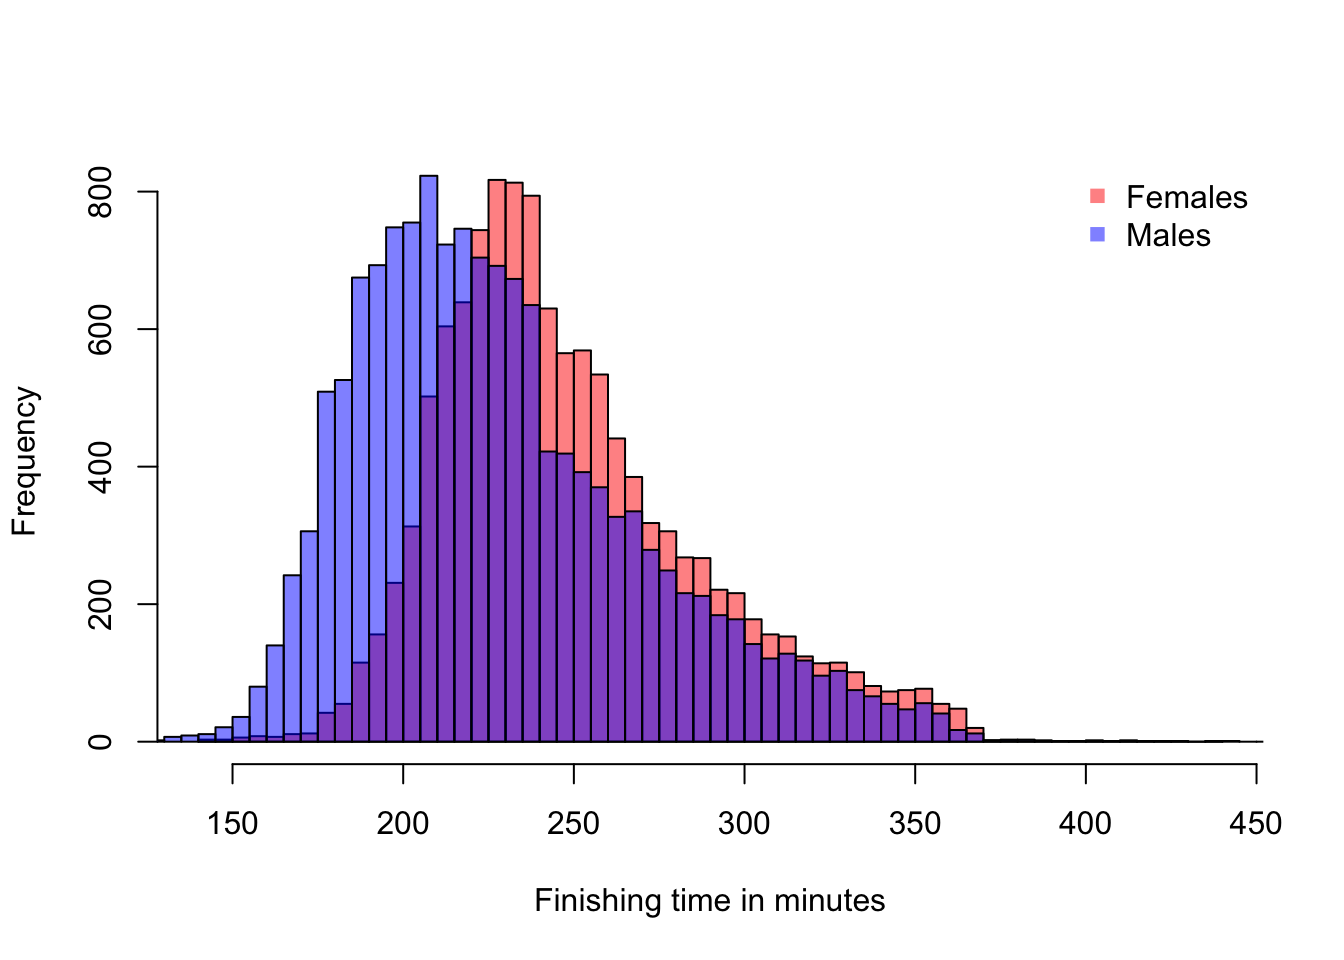
\includegraphics[width=0.9\linewidth]{carpedatum_files/figure-latex/marathon-times-1} 

}

\caption{2017 Boston Marathon finishing times}\label{fig:marathon-times}
\end{figure}

A couple of things to notice. For one thing, there is a large overlap in the two distributions. This means that there are a lot of males and females who can be matched up with similar finishing times. This observation agrees with my intution that as a below-average runner, my competitive odds against males and females may not be so different. However, there is also clearly a shift in the means of the distributions. The males are finishing faster on average. In particular, at the left end of the distribution, we are looking at the elite marathoners. Let's zoom in on that part of the distribution.

\begin{figure}

{\centering 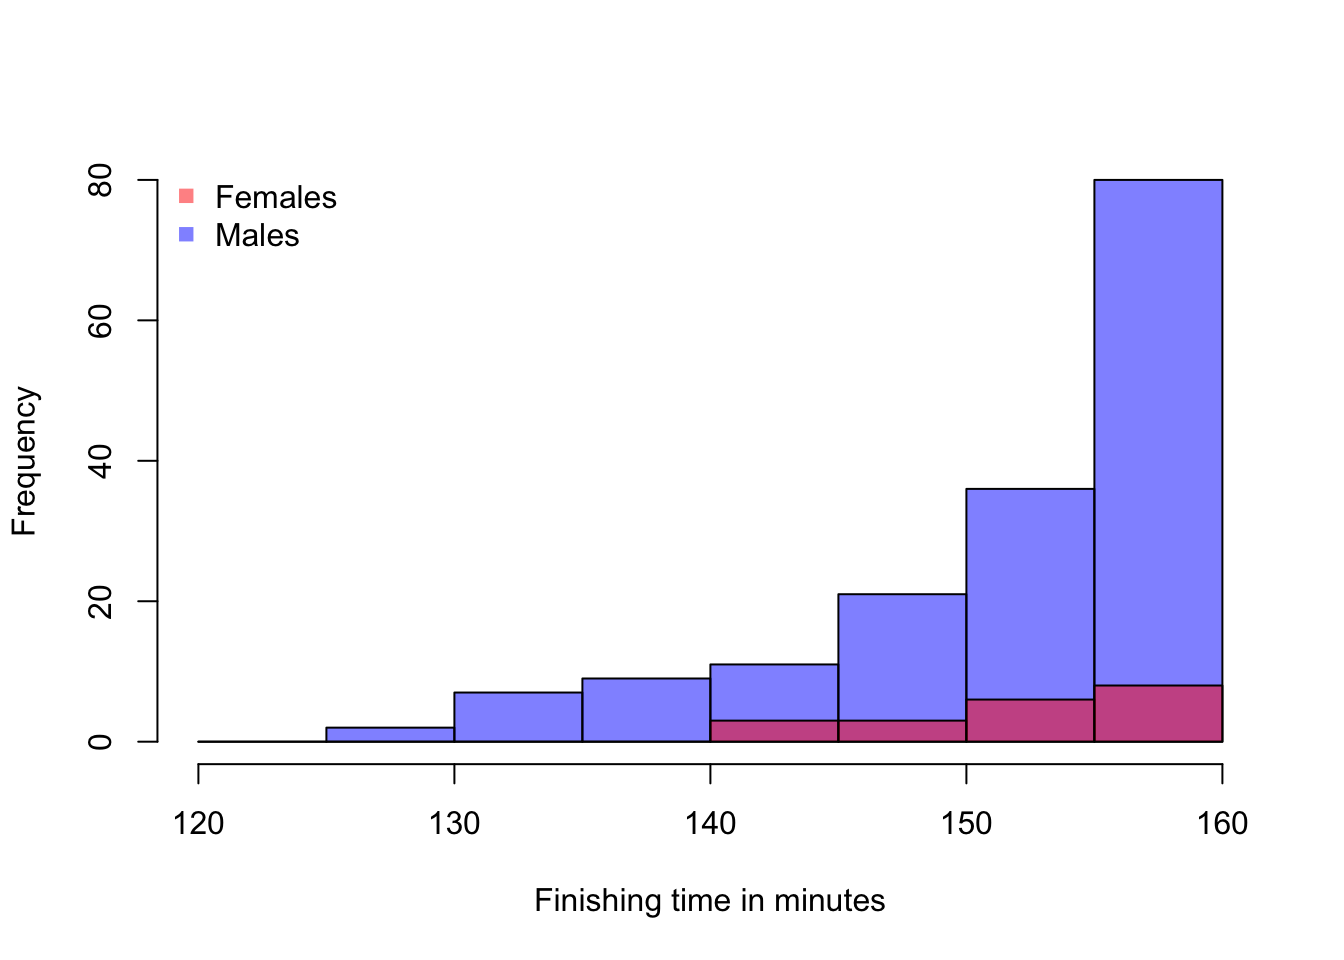
\includegraphics[width=0.9\linewidth]{carpedatum_files/figure-latex/marathon-fast-1} 

}

\caption{Fastest Runners in the 2017 Boston Marathon}\label{fig:marathon-fast}
\end{figure}

Among the elite athletes who complete the maraton in under two hours and forty minutes, the males are clearly dominant. And the top 20 finishers are all male. In such a competition, it doesn't look like a female runner will ever win.

We've created an interactive simulation for you to explore this idea further. In the simulation, you can vary the mean difference between two similar distributions and observe how often a random match-up between one member from each group (males/females) wins, and how often one of the slower group members places in the top 10.

As we can all imagine, dividing competitive running (and other sports) into separate events for males and females was designed to make the competition more interesting for the female athletes. There is still only so much room at the top. But under separate competition, the top few places for female athletes are accessible to female athletes.

Many societies now recognize that biology and gender do not align perfectly. A person whose sex at birth was male may at some point grow up to identify as a woman. This person may undergo sex reassignment or not. They may use hormone therapy. To add to the complexity, we now understand that there are sometimes differences in sex development. Trans and non-binary athletes may not fit the two-category mold that competitive sports organizations created. But there are non-cis-gendered women who want to be allowed to compete in the ``women's'' category. Is it it fair to exclude trans women from doing so? Is it fair to them? Is it fair to their cis-gendered female competitors to include anyone who identifies as a woman? Data science cannot answer this question for us, but a cold look at the data can help us at least quantify the effects of these decisions.

\hypertarget{nyc-covid-19-data}{%
\chapter{NYC COVID-19 Data}\label{nyc-covid-19-data}}

\hypertarget{prologue}{%
\section*{Prologue}\label{prologue}}
\addcontentsline{toc}{section}{Prologue}

Although Madonna may have called COVID-19 \href{https://pagesix.com/2020/03/22/madonna-calls-coronavirus-the-great-equalizer-in-bizarre-bathtub-video/}{the great equalizer} during the early stages of the outbreak in the US, others quickly highlighted some data that suggested the opposite might be true. Whenever we acknowledge the range of human experience, in the case of disease as in other cases, variance in outcomes does not necessarily imply systematic unfairness. For example, if COVID-19 is more fatal for elderly adults, as it appears to be, this is not something we would label as obviously unfair. Everyone gets old, and physical deterioration unfortunately comes with the territory. Certain chronic health conditions make people more vulnerable to COVID-19, but some of those conditions might just be the result of bad luck. We can try to make a world in which everyone has comparable access to healthcare, but we probably still can't make a world in which everyone has the same health outcomes.

However, consider the following headlines:

\begin{itemize}
\item
  \href{https://www.sciencenews.org/article/coronavirus-why-african-americans-vulnerable-covid-19-health-race}{Why African-Americans may be especially vulnerable to COVID-19}
\item
  \href{https://theintercept.com/2020/04/09/nyc-coronavirus-deaths-race-economic-divide/}{Coronavirus Numbers Reflect New York City's Deep Economic Divide}
\item
  \href{https://abcnews.go.com/Health/nyc-stark-contrast-covid-19-infection-rates-based/story?id=69920706}{In NYC, `stark contrast' in COVID-19 infection rates based on education and race}
\item
  \href{https://www.statnews.com/2020/04/09/hospitalized-covid-19-patients-differences-by-race-and-sex/}{Who gets hospitalized for Covid-19? Report shows differences by race and sex}
\end{itemize}

When adverse health outcomes are associated with income, race, and/or sex, we are much more likely to cry foul than when they are associated with age or pre-existing chronic conditions. Part of this has to do with the difference between variance among individuals, which is an unavoidable fact of life, and variance between certain classes or groups. These media reports are all suggesting that COVID-19 may not be affecting all groups with the same severity. What exactly does that mean, and is it evidence of unfairness?

New York City emerged early as the epicenter of the US outbreak, claiming over 14,000 lives by late April 2020. As specific data have became available, researchers and reporters examined counts of coronavirus infections and/or deaths by zip code and borough, by age, sex, and race. In this chapter, we will take a closer look at the data and the media reports.

Some additional reports on Coronavirus in New York:

\begin{itemize}
\tightlist
\item
  \href{https://furmancenter.org/thestoop/entry/covid-19-cases-in-new-york-city-a-neighborhood-level-analysis}{COVID-19 Cases in New York City, a Neighborhood-Level Analysis}
\item
  \href{https://gothamist.com/news/coronavirus-statistics-tracking-epidemic-new-york}{Coronavirus Statistics: Tracking The Epidemic In New York}
\end{itemize}

There are a bunch of sites that let you engage interactively with COVID-19 data. The purpose of this chapter is to show you how to build your own resource.

\hypertarget{part1}{%
\section{COVID NYC}\label{part1}}

On April 10, 2020, \href{https://abcnews.go.com/Health/nyc-stark-contrast-covid-19-infection-rates-based/story?id=69920706}{ABC News} covered an online report (by the NYU Furman Center) that examined cases of COVID-19 in New York City on a neighborhood level. Most COVID-19 data that had been coming out had been reporting on the city as a whole. The main idea here was that neighborhoods tell a different story. Data scientists call this a shift in the unit-of-analysis. The city is made of boroughs, which themselves are made up of smaller neighborhoods. So the unit of analysis could be the whole city, the boroughs of the city, or something even more fine-grained, like neighborhoods or zipcode areas. For example, some zipcodes are wealthier and some poorer. Zipcode areas also vary by racial composition. If we examine COVID-19 outcomes by neighborhood, we may be able to see patterns and associations between disease incidence and race or socio-economic variables. Indeed, the Furman Center found such associations. The ABC News report produced images like the following:

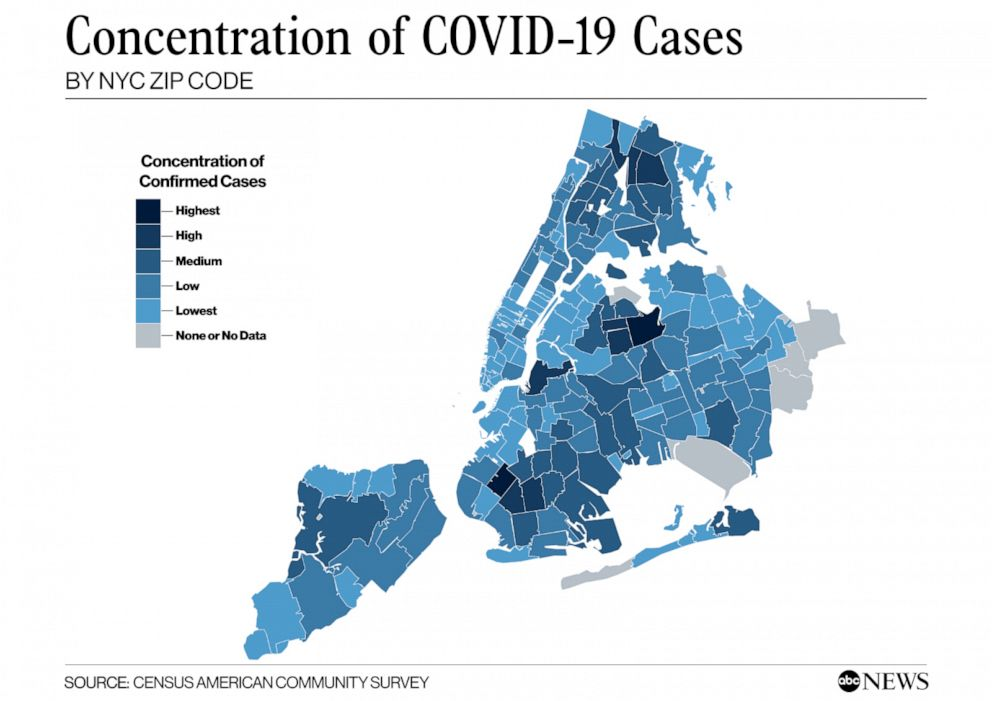
\includegraphics{images/abc_COVID19NycZip_v03_KA_hpEmbed_17x12_992.jpg}

People familiar with the layout of New York City might be able to identify low-income and largely African-American neighborhoods like Hunts Point in the South Bronx. ABC News produced a corresponding map showing the share of adults with college degree, a measure of educational attainment which the Furman Center report said was associated with disease incidence.

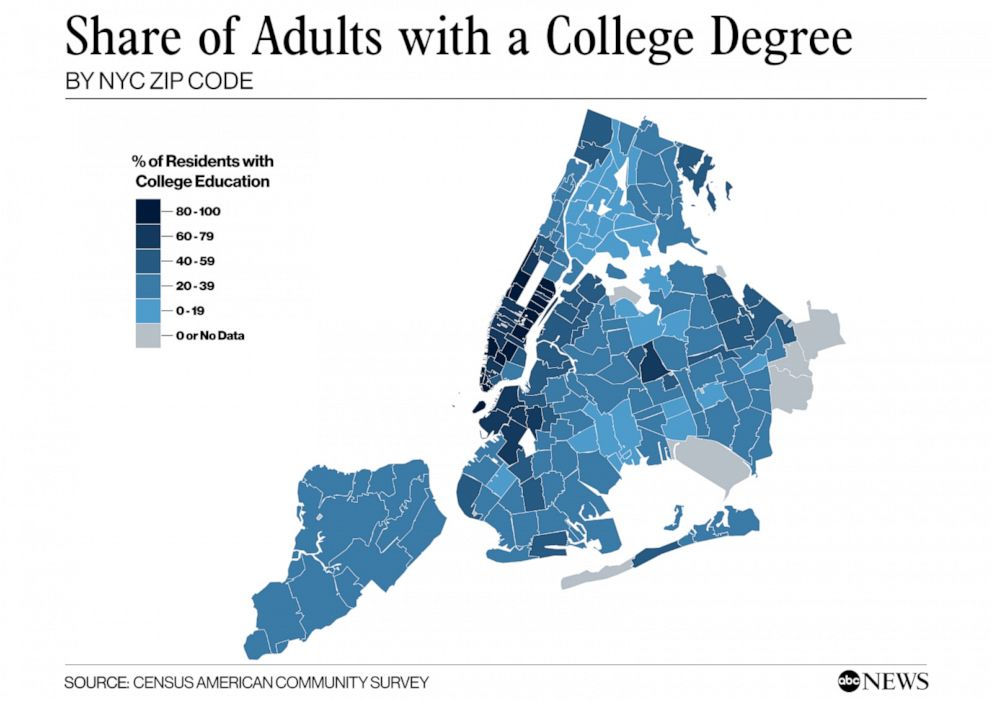
\includegraphics{images/abc_CollegeDegreeNycZip_v02_KA_hpEmbed_17x12_992.jpg}

It requires switching back and forth between these images, but the dark regions on the COVID map (higher rates of disease) seem to often correspond to the lighter regions on the college degree map (lower college share). In other words, areas with lower educational attainment seem to have higher rates of the disease. There are many possible explanations of this relationship, which are discussed in the Furman report and elsewhere.

How does one make these data visualizations? And are they the best way to ``see'' the signals in the data?

ABC News also reproduced a version of table below, showing racial composition by neighborhood. The title may confuse matters, however. In this table, multiple neighborhoods (zipcodes) are actually grouped together into five sets using \textbf{quintiles.} You take all of the zipcodes, rank-order them by COVID-19 concentration, and then select the bottom fifth, the next fifth, and so on up to the top fifth. These groups are labeled ``lowest concentration'', ``low concentration'', and so on up to ``highest concentration.''

To make matters confusing, the word ``quintile'' is often used referring to the five sets (for example, ``the lower quintile''). But strictly speaking, the quintiles are actually the cut-points. So for five groups, there are four quintiles. If you look at the table below, the cut-points/quintiles are \{3.33, 4.13, 4.77, 5.87\}. Of course, this division process can be done for a different number of \textbf{quantiles}--note the spelling--not necessarily five. A division of three groups is made by choosing two (cut-point) tertiles or terciles. The median is the 2-quantile, as it is the cut-point that divides a data set into two equal parts. Unfortunately, the naming conventions here are rather confusing, but you get used to them if you use them a lot.

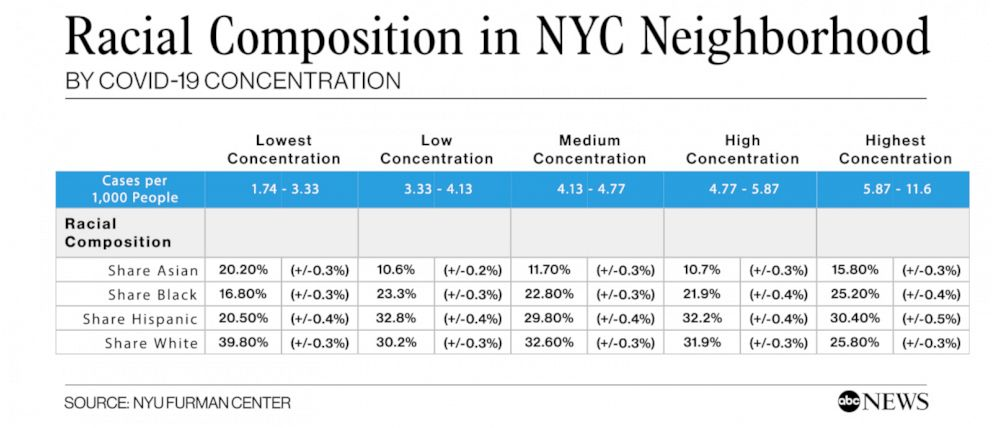
\includegraphics{images/abc_COVID19RacialComp_v02_KA_hpEmbed_37x16_992.jpg}

If you look at the table above, you may notice trends or patterns between racial composition (of these groups of neighborhoods) and COVID-19 concentration. The trends are not perfectly linear. But, for example, the proportion of Black and Hispanic people in the low-concentration neighborhoods is 37.3\%. While in the high concentration neighborhoods, this combined share is 55.6\%.

In the remainder of this tutorial, we will examine how to recreate graphs and tables like the one above from publicly available data. This will enable you to create your own versions or update the ones above with new data. We will also look at alternative representations and at some simulation-based tests to see how likely it is that such disparities might occur by chance.

Let's begin!

\hypertarget{getting-some-data}{%
\subsection*{Getting some data}\label{getting-some-data}}
\addcontentsline{toc}{subsection}{Getting some data}

In this tutorial, I will walk you through the steps of creating some of the figures and tables that go into media reports about COVID-19 outcomes. The examples here are all NYC-centric, but the methods, especially for US Census data, are completely general. The hardest part of all of this--and this is generally true about the practice of data science--is getting all of the data from different sources cleaned up and fitted together.

\hypertarget{local-data-on-covid-from-the-city-andor-state}{%
\subsection*{Local data on COVID from the city and/or state}\label{local-data-on-covid-from-the-city-andor-state}}
\addcontentsline{toc}{subsection}{Local data on COVID from the city and/or state}

For state and municipality-level COVID-19 data in New York, these are some sources:

\begin{itemize}
\tightlist
\item
  \href{https://www1.nyc.gov/site/doh/covid/covid-19-data-archive.page}{NYC data summaries}
\item
  \href{https://github.com/nychealth/coronavirus-data}{NYC Health GitHub}
\item
  \href{https://health.data.ny.gov/Health/New-York-State-Statewide-COVID-19-Testing/xdss-u53e}{NY Statewide data}
\end{itemize}

These sources have been updated daily (as of April 2021, still going). I will be working with the GitHub data as of April 23, 2020. This was early in the pandemic, just as the first big wave that hit New York City was beginning to subside. This date was about two weeks later than the Furman/ABC reports linked above. I downloaded the files from the online repository and put them into a folder on my computer. (As of April 2021, the NYC DOH data repository includes more tables, such as tabulations by race and poverty; however, these were not available in the beginning. So this information had to come from other sources. We'll get into that below, because it is widely useful.)

For starters, here I will load and view the borough-level data table.

\begin{Shaded}
\begin{Highlighting}[]
\NormalTok{nyc\_boro\_data }\OtherTok{\textless{}{-}} \FunctionTok{read.csv}\NormalTok{(}\StringTok{"data/coronavirus{-}nyc/boro.csv"}\NormalTok{, }\AttributeTok{stringsAsFactors =}\NormalTok{ F)}
\NormalTok{nyc\_boro\_data}
\end{Highlighting}
\end{Shaded}

\begin{verbatim}
##   BOROUGH_GROUP COVID_CASE_COUNT COVID_CASE_RATE
## 1     The Bronx            28875         1962.05
## 2      Brooklyn            34476         1269.58
## 3     Manhattan            16754          887.36
## 4        Queens            39856         1589.55
## 5 Staten Island             9755         1944.40
## 6      Citywide           129788              NA
\end{verbatim}

According to the documentation in the GitHub README file (a valuable source of information), this table contains rates of confirmed cases, by NYC borough of residence. Rates are:

\begin{itemize}
\tightlist
\item
  Cumulative since the start of the outbreak
\item
  Age adjusted according to \href{https://www.cdc.gov/nchs/data/statnt/statnt20.pdf}{the US 2000 standard population}
\item
  Per 100,000 people in the borough
\end{itemize}

What does age-adjusted rate mean? You can read the link, but the main idea here is to try to put all of the boroughs on equal footing in the rate per 100,000 people, even if some boroughs have an older or younger population than others. Which it turns out they do. Later, once we have borough populations, we could examine simple population-adjusted rates that are not age-adjusted and see what those look like in comparison.

If we wanted to do age-adjustment, or even simpler population adjustment, we would need to supplement this COVID data with population data, for example obtained from the US Census. Before we turn to that, let us just quickly explore the other data provided by NYC.

\begin{Shaded}
\begin{Highlighting}[]
\NormalTok{nyc\_sex\_data }\OtherTok{\textless{}{-}} \FunctionTok{read.csv}\NormalTok{(}\StringTok{"data/coronavirus{-}nyc/by{-}sex.csv"}\NormalTok{)}
\NormalTok{nyc\_sex\_data}
\end{Highlighting}
\end{Shaded}

\begin{verbatim}
##        SEX_GROUP COVID_CASE_RATE HOSPITALIZED_CASE_RATE DEATH_RATE
## 1         Female         1394.88                 324.21      77.38
## 2           Male         1702.93                 507.52     134.42
## 3 Citywide total         1545.33                 411.99     104.91
\end{verbatim}

(By the way, you may get a warning like, ``incomplete final line found'' when reading this file. You can ignore it. R is expecting each line in a .csv file to end with a newline/return. You can also just open the file and add that newline after the last row if you like).

Case and fatality rates by sex show that males are being infected and dying at significantly higher rates. Note that each of these is already adjusted to rate per 100,000.

\begin{Shaded}
\begin{Highlighting}[]
\NormalTok{nyc\_age\_data }\OtherTok{\textless{}{-}} \FunctionTok{read.csv}\NormalTok{(}\StringTok{"data/coronavirus{-}nyc/by{-}age.csv"}\NormalTok{)}
\NormalTok{nyc\_age\_data}
\end{Highlighting}
\end{Shaded}

\begin{verbatim}
##            AGE_GROUP COVID_CASE_RATE HOSPITALIZED_CASE_RATE DEATH_RATE
## 1         0-17 years          149.86                  12.91       0.17
## 2        18-44 years         1429.09                 147.79      11.28
## 3        45-64 years         2305.73                 600.33      96.69
## 4        65-74 years         2351.39                1123.27     311.68
## 5 75 and older years         2728.10                1682.16     778.83
## 6     Citywide total         1545.33                 411.99     104.91
\end{verbatim}

Age-level data show a few interesting features. For one, children are barely even getting infected. Among adults, infection rates are slightly higher for older adults, but death rates are much higher. We could derive a measure of case fatality rate (CFR) as follows:

\begin{Shaded}
\begin{Highlighting}[]
\NormalTok{nyc\_age\_data}\SpecialCharTok{$}\NormalTok{CFR }\OtherTok{\textless{}{-}} \FunctionTok{round}\NormalTok{(nyc\_age\_data}\SpecialCharTok{$}\NormalTok{DEATH\_RATE}\SpecialCharTok{/}\NormalTok{nyc\_age\_data}\SpecialCharTok{$}\NormalTok{COVID\_CASE\_RATE, }\DecValTok{3}\NormalTok{)}
\NormalTok{nyc\_age\_data}
\end{Highlighting}
\end{Shaded}

\begin{verbatim}
##            AGE_GROUP COVID_CASE_RATE HOSPITALIZED_CASE_RATE DEATH_RATE   CFR
## 1         0-17 years          149.86                  12.91       0.17 0.001
## 2        18-44 years         1429.09                 147.79      11.28 0.008
## 3        45-64 years         2305.73                 600.33      96.69 0.042
## 4        65-74 years         2351.39                1123.27     311.68 0.133
## 5 75 and older years         2728.10                1682.16     778.83 0.285
## 6     Citywide total         1545.33                 411.99     104.91 0.068
\end{verbatim}

From this we see that adults 75 and older have a 28.5\% chance of dying from COVID-19, compared to a 4.2\% for adults between 45-64.

\textbf{Exercise}: compute the case fatality rate by sex.

Since I'm going to be using this method later, there is another way to add a new CFR variable to the table using the \texttt{mutate} function in the \texttt{dplyr} package. It looks slightly more complicated, but it has benefits which I won't get into now. The important thing here is just to recognize that there are different ways of achieving the same ends.

\begin{Shaded}
\begin{Highlighting}[]
\CommentTok{\# the way from before}
\CommentTok{\# nyc\_age\_data$CFR \textless{}{-} round(nyc\_age\_data$DEATH\_RATE/nyc\_age\_data$COVID\_CASE\_RATE, 3)}

\CommentTok{\# another way using dplyr}
\NormalTok{nyc\_age\_data }\OtherTok{\textless{}{-}}\NormalTok{ nyc\_age\_data }\SpecialCharTok{\%\textgreater{}\%} \FunctionTok{mutate}\NormalTok{(}\AttributeTok{CFR =} \FunctionTok{round}\NormalTok{(DEATH\_RATE}\SpecialCharTok{/}\NormalTok{COVID\_CASE\_RATE,}\DecValTok{3}\NormalTok{))}
\NormalTok{nyc\_age\_data}
\end{Highlighting}
\end{Shaded}

\begin{verbatim}
##            AGE_GROUP COVID_CASE_RATE HOSPITALIZED_CASE_RATE DEATH_RATE   CFR
## 1         0-17 years          149.86                  12.91       0.17 0.001
## 2        18-44 years         1429.09                 147.79      11.28 0.008
## 3        45-64 years         2305.73                 600.33      96.69 0.042
## 4        65-74 years         2351.39                1123.27     311.68 0.133
## 5 75 and older years         2728.10                1682.16     778.83 0.285
## 6     Citywide total         1545.33                 411.99     104.91 0.068
\end{verbatim}

The most captivating data set provided by the city (hence the images we started out with) is probably the zipcode-level data, the first few rows of which look like this:

\begin{Shaded}
\begin{Highlighting}[]
\NormalTok{nyc\_zipcode\_data }\OtherTok{\textless{}{-}} \FunctionTok{read.csv}\NormalTok{(}\StringTok{"data/coronavirus{-}nyc/tests{-}by{-}zcta.csv"}\NormalTok{)}
\FunctionTok{head}\NormalTok{(nyc\_zipcode\_data,}\DecValTok{20}\NormalTok{)}
\end{Highlighting}
\end{Shaded}

\begin{verbatim}
##    MODZCTA Positive Total zcta_cum.perc_pos
## 1       NA     1864  2078             89.70
## 2    10001      260   571             45.53
## 3    10002      712  1358             52.43
## 4    10003      347   830             41.81
## 5    10004       24    64             37.50
## 6    10005       44   137             32.12
## 7    10006       14    54             25.93
## 8    10007       40   130             30.77
## 9    10009      518  1180             43.90
## 10   10010      201   561             35.83
## 11   10011      394   852             46.24
## 12   10012      116   330             35.15
## 13   10013      179   426             42.02
## 14   10014      233   529             44.05
## 15   10016      502  1197             41.94
## 16   10017      107   310             34.52
## 17   10018      168   375             44.80
## 18   10019      441   999             44.14
## 19   10021      431  1148             37.54
## 20   10022      250   668             37.43
\end{verbatim}

Notice that the first row is missing a zipcode. Presumably these are COVID tests for which we do not know where the people who were tested actually reside.

For each other row, we have a zipcode, the number of positive tests, the number of total tests, and the percent positive.

\textbf{Exercise}: Which of these expressions should give the percent positive tests?

\begin{verbatim}
nyc_zipcode_data$Total/nyc_zipcode_data$Positive*100
nyc_zipcode_data$Positive/nyc_zipcode_data$Total
nyc_zipcode_data$Positive/nyc_zipcode_data$Total*100
(nyc_zipcode_data$Total-nyc_zipcode_data$Positive)
(nyc_zipcode_data$Total-nyc_zipcode_data$Positive)*100
\end{verbatim}

Now you might want to keep the first row, the one with the missing zipcode, in your data. But I would rather remove it now, because I'm going to try to add information to this zipcode table down the line. While I'm at it, I will also rename the column ``MODZCTA'' with ``zipcode.''

\begin{Shaded}
\begin{Highlighting}[]
\NormalTok{nyc\_zipcode\_data }\OtherTok{\textless{}{-}} \FunctionTok{na.omit}\NormalTok{(nyc\_zipcode\_data)}
\FunctionTok{names}\NormalTok{(nyc\_zipcode\_data)[}\DecValTok{1}\NormalTok{] }\OtherTok{\textless{}{-}} \StringTok{"zipcode"}
\FunctionTok{head}\NormalTok{(nyc\_zipcode\_data)}
\end{Highlighting}
\end{Shaded}

\begin{verbatim}
##   zipcode Positive Total zcta_cum.perc_pos
## 2   10001      260   571             45.53
## 3   10002      712  1358             52.43
## 4   10003      347   830             41.81
## 5   10004       24    64             37.50
## 6   10005       44   137             32.12
## 7   10006       14    54             25.93
\end{verbatim}

There are a couple more tables included in the GitHub repository, for example ones showing the daily tracking of new cases, hospitalizations, and deaths. But as we are focusing on the neighborhood level counts, I will leave them out of these notes.

In the next part of the series, we will get started with US Census data.

\hypertarget{part2}{%
\section{Getting started with US Census data}\label{part2}}

To get census data, you can go to (\url{https://data.census.gov/}), but be warned: it is a big maze and not that easy to navigate. What the pros who make media reports do (probably) is use the US Census API to make specific requests for data. If you use it a lot, you will need an API key. This is easy enough to get, but you need to \href{https://api.census.gov/data/key_signup.html}{request one here}. Once you have a key, you can declare it in your R code or, better for security/code-sharing, embed it in a .Renviron file.

Here I will load the \texttt{censusapi} package (and also \texttt{dplyr} while I'm at it), and load my key. You can modify this line with your key. If you don't have one, some or all of the code below will still work if you comment out the \texttt{key=myKey}. Without an API key, however, there is a limit to the size and number of queries per IP address.

\begin{Shaded}
\begin{Highlighting}[]
\FunctionTok{library}\NormalTok{(censusapi)}
\FunctionTok{library}\NormalTok{(dplyr)}
\CommentTok{\# comment this out if you want to proceed without a key}
\CommentTok{\# myKey = Sys.getenv("CENSUS\_KEY") \#store your key in .Renviron}
\end{Highlighting}
\end{Shaded}

More importantly, when it comes to census data, you need to know what you're asking for. That means you need to know which data sets, which variables, which geographic units, etc. A brief introductory \href{https://www.census.gov/content/dam/Census/data/developers/api-user-guide/api-guide.pdf}{API users guide can be found here}. It's 20 pages long. You can just follow along here if you want some examples.

We will be interested in the \href{https://www.census.gov/data/developers/data-sets/acs-5year.html}{American Community Survey 5-Year data} (aka ACS5) which provides estimates aggregated over a 5-year period, revisited every two years. The last published data set, i.e., the most current one available, is from 2018.

\hypertarget{census-variables}{%
\subsection*{Census Variables}\label{census-variables}}
\addcontentsline{toc}{subsection}{Census Variables}

There are something like 20,000 variables available in ACS, and these can be retrieved through queries invidividually or in groups. Some useful groups for our analysis are the following

\begin{itemize}
\tightlist
\item
  B01001 SEX BY AGE

  \begin{itemize}
  \tightlist
  \item
    This has a lot of subcategories, such as Male 5-9 Years, Male 10-14 years, etc.
  \end{itemize}
\item
  B02001 RACE (disregards Hispanic or Latino Origin)
\item
  B03002 HISPANIC OR LATINO ORIGIN BY RACE\\
\item
  B19013 MEDIAN HOUSEHOLD INCOME IN THE PAST 12 MONTHS
\end{itemize}

For each group, a list of variables can be found on a corresponding census.gov website. For example, to find the variables in the SEX BY AGE group, you can go to \url{https://api.census.gov/data/2018/acs/acs5/groups/B01001.html} (notice the URL ending is the same as the group). There you will find variables such as

\begin{itemize}
\tightlist
\item
  B01001\_001E Estimate!!Total
\item
  B01001\_002E Estimate!!Total!!Male
\item
  B01001\_026E Estimate!!Total!!Female
\end{itemize}

And many more. Variables that end in E are estimates. For each one there is often a margin of error, which is the same code ending in M instead of E. Finally for both estimates and margins of error, there may be annotations (e.g.~B01001\_002EA and B01001\_002MA), if these numbers are missing or not straightforward. Details about annotation meanings can be found \href{https://www.census.gov/data/developers/data-sets/acs-1year/notes-on-acs-estimate-and-annotation-values.html}{here}. This is just an overview of what the ACS5 variable names look like.

\hypertarget{geography-units}{%
\subsection*{Geography Units}\label{geography-units}}
\addcontentsline{toc}{subsection}{Geography Units}

Census data are available at many levels related to geographical units. The smallest unit is called a census ``block'' and typically covers between 600 and 3000 people. A collection of blocks forms a census tract (2500 to 8000 people). But US states are also divided into counties, and both state and county identifiers can be used as region selectors. Note that to use the Census API, one has to use numerical identifiers for states and counties. For example, the borough of Brooklyn is actually Kings County, New York, which is county 047 in state 36. And yes, you have to include all three digits, including the leading zero, to identify individual counties. Zipcode tabulation areas (aka ZCTA) is another option, wherein you specify the five-digit zip code. We will want to use that, because NYC provided COVID-19 testing data at the zipcode level.

\hypertarget{borough-level-data}{%
\subsubsection*{Borough-level data}\label{borough-level-data}}
\addcontentsline{toc}{subsubsection}{Borough-level data}

First, let's retrieve some data about the five boroughs. Let's start with the simplest example and get the size of each borough population.

We will need to request the variable B01001\_001E, which is the total population estimate.

\begin{Shaded}
\begin{Highlighting}[]
\NormalTok{acs\_boro\_population }\OtherTok{\textless{}{-}} \FunctionTok{getCensus}\NormalTok{(}\AttributeTok{name =} \StringTok{"acs/acs5"}\NormalTok{,}
                         \AttributeTok{vintage =} \DecValTok{2018}\NormalTok{,}
                         \AttributeTok{vars =} \FunctionTok{c}\NormalTok{(}\StringTok{"NAME"}\NormalTok{, }\StringTok{"B01001\_001E"}\NormalTok{),}
                         \AttributeTok{region =} \StringTok{"county:005,047,061,081,085"}\NormalTok{,}
                         \AttributeTok{regionin =} \StringTok{"state:36"}\NormalTok{ , }\AttributeTok{key =}\NormalTok{ myKey}
\NormalTok{                         )}

\NormalTok{acs\_boro\_population}
\end{Highlighting}
\end{Shaded}

\begin{verbatim}
##   state county                      NAME B01001_001E
## 1    36    081   Queens County, New York     2298513
## 2    36    061 New York County, New York     1632480
## 3    36    005    Bronx County, New York     1437872
## 4    36    047    Kings County, New York     2600747
## 5    36    085 Richmond County, New York      474101
\end{verbatim}

Cool! We've established that we can pull some borough-level information from the US Census to complement data provided by the city or state. Note that the two tables, the one from NYC and the one from the census, don't exactly match up. For one thing, the county names do not align with the borough names.

\hypertarget{using-named-vectors-as-look-up-tools}{%
\subsubsection*{Using named vectors as look-up tools}\label{using-named-vectors-as-look-up-tools}}
\addcontentsline{toc}{subsubsection}{Using named vectors as look-up tools}

Now, we can fix this by hand, but there are good ways and less good ways to do this. Ideally, we create a look-up table which we can reuse whenever we need to switch between borough and county names. For those familiar with database ``join'' operations, it is indeed possible to use joins in R. However, a simple way to just convert between two different representations (e.g., country name and borough name) is to use ``named vectors'' in R. Here's how:

\begin{Shaded}
\begin{Highlighting}[]
\CommentTok{\# Borough names}
\NormalTok{boroNames }\OtherTok{\textless{}{-}}\NormalTok{ nyc\_boro\_data}\SpecialCharTok{$}\NormalTok{BOROUGH\_GROUP[}\DecValTok{1}\SpecialCharTok{:}\DecValTok{5}\NormalTok{]}
\CommentTok{\# County names}
\NormalTok{countyNames }\OtherTok{\textless{}{-}}\NormalTok{ acs\_boro\_population}\SpecialCharTok{$}\NormalTok{NAME}

\CommentTok{\# combine, but note that the order is not the same! So we\textquotesingle{}ll reorder}
\NormalTok{boro2county }\OtherTok{\textless{}{-}} \FunctionTok{data.frame}\NormalTok{(}\AttributeTok{Borough=}\NormalTok{boroNames, }\AttributeTok{County=}\NormalTok{countyNames[}\FunctionTok{c}\NormalTok{(}\DecValTok{3}\NormalTok{,}\DecValTok{4}\NormalTok{,}\DecValTok{2}\NormalTok{,}\DecValTok{1}\NormalTok{,}\DecValTok{5}\NormalTok{)], }
                          \AttributeTok{stringsAsFactors =} \ConstantTok{FALSE}\NormalTok{)}

\CommentTok{\# create two \textquotesingle{}named vectors\textquotesingle{}}
\CommentTok{\# one for getting the borough}
\NormalTok{getBoro }\OtherTok{\textless{}{-}}\NormalTok{ boro2county}\SpecialCharTok{$}\NormalTok{Borough}
\FunctionTok{names}\NormalTok{(getBoro) }\OtherTok{\textless{}{-}}\NormalTok{ boro2county}\SpecialCharTok{$}\NormalTok{County}

\CommentTok{\# one for getting the county}
\NormalTok{getCounty }\OtherTok{\textless{}{-}}\NormalTok{ boro2county}\SpecialCharTok{$}\NormalTok{County}
\FunctionTok{names}\NormalTok{(getCounty) }\OtherTok{\textless{}{-}}\NormalTok{ boro2county}\SpecialCharTok{$}\NormalTok{Borough}
\end{Highlighting}
\end{Shaded}

Here's is one way we can use this new lookup table. Note that \texttt{getBoro} is not a function (it is a named vector). So we use square brackets to index it, not parentheses.

\begin{Shaded}
\begin{Highlighting}[]
\NormalTok{getBoro[}\StringTok{"Richmond County, New York"}\NormalTok{]}
\end{Highlighting}
\end{Shaded}

\begin{verbatim}
## Richmond County, New York 
##           "Staten Island"
\end{verbatim}

\begin{Shaded}
\begin{Highlighting}[]
\NormalTok{getCounty[}\StringTok{"Brooklyn"}\NormalTok{]}
\end{Highlighting}
\end{Shaded}

\begin{verbatim}
##                 Brooklyn 
## "Kings County, New York"
\end{verbatim}

\begin{Shaded}
\begin{Highlighting}[]
\NormalTok{acs\_boro\_population}\SpecialCharTok{$}\NormalTok{Borough }\OtherTok{\textless{}{-}}\NormalTok{ getBoro[acs\_boro\_population}\SpecialCharTok{$}\NormalTok{NAME]}
\NormalTok{acs\_boro\_population}
\end{Highlighting}
\end{Shaded}

\begin{verbatim}
##   state county                      NAME B01001_001E       Borough
## 1    36    081   Queens County, New York     2298513        Queens
## 2    36    061 New York County, New York     1632480     Manhattan
## 3    36    005    Bronx County, New York     1437872     The Bronx
## 4    36    047    Kings County, New York     2600747      Brooklyn
## 5    36    085 Richmond County, New York      474101 Staten Island
\end{verbatim}

All that remains is that annoying variable name B01001\_001E for Total Population. We should definitely fix this, and there are a few ways to do it. The following may seem like a long-winded way to go about it, but it has the benefit that it will work no matter where the variable B01001\_001E appears. It won't accidentally change the wrong column name, and it won't do anything at all if the variable you are trying to rename doesn't exist.

\begin{Shaded}
\begin{Highlighting}[]
\FunctionTok{names}\NormalTok{(acs\_boro\_population)[}\FunctionTok{which}\NormalTok{(}\FunctionTok{names}\NormalTok{(acs\_boro\_population)}\SpecialCharTok{==}\StringTok{"B01001\_001E"}\NormalTok{)] }\OtherTok{\textless{}{-}} \StringTok{"Total\_Pop"}
\FunctionTok{names}\NormalTok{(acs\_boro\_population)[}\FunctionTok{which}\NormalTok{(}\FunctionTok{names}\NormalTok{(acs\_boro\_population)}\SpecialCharTok{==}\StringTok{"NAME"}\NormalTok{)] }\OtherTok{\textless{}{-}} \StringTok{"countyName"}
\NormalTok{acs\_boro\_population}
\end{Highlighting}
\end{Shaded}

\begin{verbatim}
##   state county                countyName Total_Pop       Borough
## 1    36    081   Queens County, New York   2298513        Queens
## 2    36    061 New York County, New York   1632480     Manhattan
## 3    36    005    Bronx County, New York   1437872     The Bronx
## 4    36    047    Kings County, New York   2600747      Brooklyn
## 5    36    085 Richmond County, New York    474101 Staten Island
\end{verbatim}

(If you're wondering whether we could have used named vectors to convert between the ACS names, like B01001\_001E, and simple names like ``Total\_Pop'', then yes, but you're getting ahead of me. Once we have more than a few of these variables, that would indeed be a good idea.)

With this in hand, we can now combine our NYC COVID-19 data with our Census data. Let's bring back our first borough table:

\begin{Shaded}
\begin{Highlighting}[]
\NormalTok{nyc\_boro\_data}
\end{Highlighting}
\end{Shaded}

\begin{verbatim}
##   BOROUGH_GROUP COVID_CASE_COUNT COVID_CASE_RATE
## 1     The Bronx            28875         1962.05
## 2      Brooklyn            34476         1269.58
## 3     Manhattan            16754          887.36
## 4        Queens            39856         1589.55
## 5 Staten Island             9755         1944.40
## 6      Citywide           129788              NA
\end{verbatim}

We will make some judicious use of dplyr here to simplify the outcome. Mostly, we want to get rid of unnecessary columns from the ACS table (using \texttt{select}), and then use \texttt{join()} to merge the two tables. The advantage of the pipe operatore \texttt{\%\textgreater{}\%} is that it allows us to think of our data as going through a flow of operations. First we take our table of data, then we select the columns we care about, then we combine it with our other table (the NYC data on COVID-19):

\begin{Shaded}
\begin{Highlighting}[]
\NormalTok{boro\_join }\OtherTok{\textless{}{-}}\NormalTok{ acs\_boro\_population }\SpecialCharTok{\%\textgreater{}\%} \FunctionTok{select}\NormalTok{(Borough, countyName, Total\_Pop) }\SpecialCharTok{\%\textgreater{}\%} 
  \FunctionTok{left\_join}\NormalTok{(nyc\_boro\_data, }\AttributeTok{by=}\FunctionTok{c}\NormalTok{(}\StringTok{"Borough"} \OtherTok{=}  \StringTok{"BOROUGH\_GROUP"}\NormalTok{))}
\NormalTok{boro\_join}
\end{Highlighting}
\end{Shaded}

\begin{verbatim}
##         Borough                countyName Total_Pop COVID_CASE_COUNT
## 1        Queens   Queens County, New York   2298513            39856
## 2     Manhattan New York County, New York   1632480            16754
## 3     The Bronx    Bronx County, New York   1437872            28875
## 4      Brooklyn    Kings County, New York   2600747            34476
## 5 Staten Island Richmond County, New York    474101             9755
##   COVID_CASE_RATE
## 1         1589.55
## 2          887.36
## 3         1962.05
## 4         1269.58
## 5         1944.40
\end{verbatim}

Woohoo! (I'm keeping countyName for later. You'll see why.)

\textbf{Worked Example}: Compute the population adjusted rate per 100,000 people using population data from the census. How does it differ from the age-adjusted rate?

We can use our population estimates (keep in mind that these are 5-year averages as of 2018) to derive our own rate-per-100,000 as follows

\begin{Shaded}
\begin{Highlighting}[]
\NormalTok{boro\_join}\SpecialCharTok{$}\NormalTok{RATE\_100K }\OtherTok{\textless{}{-}}  \FunctionTok{round}\NormalTok{(boro\_join}\SpecialCharTok{$}\NormalTok{COVID\_CASE\_COUNT}\SpecialCharTok{/}\NormalTok{boro\_join}\SpecialCharTok{$}\NormalTok{Total\_Pop }\SpecialCharTok{*} \DecValTok{100000}\NormalTok{, }\DecValTok{2}\NormalTok{)}
\NormalTok{boro\_join }\SpecialCharTok{\%\textgreater{}\%} \FunctionTok{select}\NormalTok{(Borough, COVID\_CASE\_RATE, RATE\_100K)}
\end{Highlighting}
\end{Shaded}

\begin{verbatim}
##         Borough COVID_CASE_RATE RATE_100K
## 1        Queens         1589.55   1733.99
## 2     Manhattan          887.36   1026.29
## 3     The Bronx         1962.05   2008.18
## 4      Brooklyn         1269.58   1325.62
## 5 Staten Island         1944.40   2057.58
\end{verbatim}

You'll notice that our rate, which is not age-adjusted, differs somewhat from the NYC rate, which is age-adjusted. Aside from age-adjustment, it is possible that our population numbers (based on 5-year averages) are different from the latest NYC populations estimates. If our population numbers are lower, then our rates would be higher. Or the difference could be a result of the age-adjustment formula.

\hypertarget{more-variables-income-age-and-race}{%
\subsubsection*{More variables: income, age, and race}\label{more-variables-income-age-and-race}}
\addcontentsline{toc}{subsubsection}{More variables: income, age, and race}

To request the median household income we will request the variable ``B19013\_001E'' (intuitive, right?) Alternatively, the variable B20017\_001E is earnings per person not by household. Why not examine both?

\begin{Shaded}
\begin{Highlighting}[]
\NormalTok{acs\_boro\_income }\OtherTok{\textless{}{-}} \FunctionTok{getCensus}\NormalTok{(}\AttributeTok{name =} \StringTok{"acs/acs5"}\NormalTok{,}
                         \AttributeTok{vintage =} \DecValTok{2018}\NormalTok{,}
                         \AttributeTok{vars =} \FunctionTok{c}\NormalTok{(}\StringTok{"NAME"}\NormalTok{, }\StringTok{"B19013\_001E"}\NormalTok{, }\StringTok{"B20017\_001E"}\NormalTok{),}
                         \AttributeTok{region =} \StringTok{"county:005,047,061,081,085"}\NormalTok{,}
                         \AttributeTok{regionin =} \StringTok{"state:36"}\NormalTok{ , }\AttributeTok{key =}\NormalTok{ myKey}
\NormalTok{                         )}

\FunctionTok{names}\NormalTok{(acs\_boro\_income)[}\FunctionTok{which}\NormalTok{(}\FunctionTok{names}\NormalTok{(acs\_boro\_income)}\SpecialCharTok{==}\StringTok{"B19013\_001E"}\NormalTok{)] }\OtherTok{\textless{}{-}} \StringTok{"Median\_HH\_Income"}
\FunctionTok{names}\NormalTok{(acs\_boro\_income)[}\FunctionTok{which}\NormalTok{(}\FunctionTok{names}\NormalTok{(acs\_boro\_income)}\SpecialCharTok{==}\StringTok{"B20017\_001E"}\NormalTok{)] }\OtherTok{\textless{}{-}} \StringTok{"Median\_Income"}
\NormalTok{acs\_boro\_income}
\end{Highlighting}
\end{Shaded}

\begin{verbatim}
##   state county                      NAME Median_HH_Income Median_Income
## 1    36    081   Queens County, New York            64987         36381
## 2    36    061 New York County, New York            82459         59620
## 3    36    005    Bronx County, New York            38085         27074
## 4    36    047    Kings County, New York            56015         37123
## 5    36    085 Richmond County, New York            79267         46586
\end{verbatim}

There it is, five-year averages, inflation-adjusted for 2018 dollars, by borough. (If you see one-year estimates, they may be a bit higher than these numbers, if wages went up faster than inflation).

We can add these new income variables to the table we've started to build

\begin{Shaded}
\begin{Highlighting}[]
\CommentTok{\# Note that I am renaming NAME to countyName in the select(), }
\CommentTok{\# so I didn\textquotesingle{}t have to do it ahead of time}

\FunctionTok{left\_join}\NormalTok{(boro\_join, }
\NormalTok{          acs\_boro\_income }\SpecialCharTok{\%\textgreater{}\%} \FunctionTok{select}\NormalTok{(}\AttributeTok{countyName=}\NormalTok{NAME, Median\_HH\_Income, Median\_Income), }
          \AttributeTok{by=}\StringTok{"countyName"}\NormalTok{)}
\end{Highlighting}
\end{Shaded}

\begin{verbatim}
##         Borough                countyName Total_Pop COVID_CASE_COUNT
## 1        Queens   Queens County, New York   2298513            39856
## 2     Manhattan New York County, New York   1632480            16754
## 3     The Bronx    Bronx County, New York   1437872            28875
## 4      Brooklyn    Kings County, New York   2600747            34476
## 5 Staten Island Richmond County, New York    474101             9755
##   COVID_CASE_RATE RATE_100K Median_HH_Income Median_Income
## 1         1589.55   1733.99            64987         36381
## 2          887.36   1026.29            82459         59620
## 3         1962.05   2008.18            38085         27074
## 4         1269.58   1325.62            56015         37123
## 5         1944.40   2057.58            79267         46586
\end{verbatim}

In the next part of the series, we will keep assembling more variables related to age and race. We will also eventually change our unit of analysis to zipcode tabulation areas.

\hypertarget{part3}{%
\section{More (and messier) Census data}\label{part3}}

\hypertarget{exploring-the-acs-data}{%
\subsection*{Exploring the ACS data}\label{exploring-the-acs-data}}
\addcontentsline{toc}{subsection}{Exploring the ACS data}

So far, we have been selecting one or two variables at a time, because we knew what we were looking for. Sometimes, though, you're not exactly sure what variables are in the data. Moreoever, since many of the ACS tables combine categories (such as SEX BY AGE), the number of variables grows exponentially (e.g., as the number of SEX categories times the number of AGE categories). Add to that the margin-of-error and annotation variables, and the list gets overwhelming fast.

Even data from the SEX BY AGE group (B01001), which seems simple, is rather complicated-looking! I will walk through it deliberately, as I would do if I were exploring the data for the first time and not sure what I was going to find.

First, I will use the function \texttt{listCensusMetadata} to request all of the variables in the group B01001 and see what we see.

\begin{Shaded}
\begin{Highlighting}[]
\CommentTok{\# a list of groups can be found here; there are 1135 of them!}
\CommentTok{\# acs\_groups \textless{}{-} listCensusMetadata(name = "acs/acs5", vintage = 2018, type = "groups")}
\CommentTok{\# head(acs\_groups)}

\CommentTok{\# here are the variables in the SEX BY AGE group}
\NormalTok{group\_B01001 }\OtherTok{\textless{}{-}} \FunctionTok{listCensusMetadata}\NormalTok{(}\AttributeTok{name =} \StringTok{"acs/acs5"}\NormalTok{,}
                                   \AttributeTok{vintage =} \DecValTok{2018}\NormalTok{,}
                                   \AttributeTok{type =} \StringTok{"variables"}\NormalTok{,}
                                   \AttributeTok{group =} \StringTok{"B01001"}\NormalTok{)}
\FunctionTok{head}\NormalTok{(group\_B01001[}\FunctionTok{order}\NormalTok{(group\_B01001}\SpecialCharTok{$}\NormalTok{name),], }\DecValTok{15}\NormalTok{)}
\end{Highlighting}
\end{Shaded}

\begin{verbatim}
##             name                                                     label
## 139  B01001_001E                                           Estimate!!Total
## 41  B01001_001EA                             Annotation of Estimate!!Total
## 140  B01001_001M                                    Margin of Error!!Total
## 42  B01001_001MA                      Annotation of Margin of Error!!Total
## 137  B01001_002E                                     Estimate!!Total!!Male
## 53  B01001_002EA                       Annotation of Estimate!!Total!!Male
## 138  B01001_002M                              Margin of Error!!Total!!Male
## 54  B01001_002MA                Annotation of Margin of Error!!Total!!Male
## 143  B01001_003E                      Estimate!!Total!!Male!!Under 5 years
## 50  B01001_003EA        Annotation of Estimate!!Total!!Male!!Under 5 years
## 144  B01001_003M               Margin of Error!!Total!!Male!!Under 5 years
## 51  B01001_003MA Annotation of Margin of Error!!Total!!Male!!Under 5 years
## 141  B01001_004E                       Estimate!!Total!!Male!!5 to 9 years
## 52  B01001_004EA         Annotation of Estimate!!Total!!Male!!5 to 9 years
## 142  B01001_004M                Margin of Error!!Total!!Male!!5 to 9 years
##        concept predicateType  group limit predicateOnly
## 139 SEX BY AGE           int B01001     0          TRUE
## 41  SEX BY AGE        string B01001     0          TRUE
## 140 SEX BY AGE           int B01001     0          TRUE
## 42  SEX BY AGE        string B01001     0          TRUE
## 137 SEX BY AGE           int B01001     0          TRUE
## 53  SEX BY AGE        string B01001     0          TRUE
## 138 SEX BY AGE           int B01001     0          TRUE
## 54  SEX BY AGE        string B01001     0          TRUE
## 143 SEX BY AGE           int B01001     0          TRUE
## 50  SEX BY AGE        string B01001     0          TRUE
## 144 SEX BY AGE           int B01001     0          TRUE
## 51  SEX BY AGE        string B01001     0          TRUE
## 141 SEX BY AGE           int B01001     0          TRUE
## 52  SEX BY AGE        string B01001     0          TRUE
## 142 SEX BY AGE           int B01001     0          TRUE
\end{verbatim}

Ugh. Note that our table of variables here includes variable name, label, and type. For type, we have ``int'' for integers (numbers) and ``string'' which is the computational shorthand for ``string of characters.'' This is the variable-type used for words and sentences as well as passwords or other random strings of characters.

To make the results more readable, we can try identify the pattern in the order of the variables. First, let's observe the following. The numbers after the group name are just increasing from 001, 002, and so on. We might want to look at the middle of this list, e.g, from 020 to 030, which we can do as follows:

\begin{Shaded}
\begin{Highlighting}[]
\NormalTok{myVars }\OtherTok{\textless{}{-}} \FunctionTok{paste0}\NormalTok{(}\StringTok{"B01001\_0"}\NormalTok{,}\FunctionTok{sprintf}\NormalTok{(}\StringTok{"\%02d"}\NormalTok{, }\DecValTok{20}\SpecialCharTok{:}\DecValTok{30}\NormalTok{), }\StringTok{"E"}\NormalTok{)}
\NormalTok{group\_B01001 }\SpecialCharTok{\%\textgreater{}\%} \FunctionTok{filter}\NormalTok{(name }\SpecialCharTok{\%in\%}\NormalTok{ myVars) }\SpecialCharTok{\%\textgreater{}\%} \FunctionTok{arrange}\NormalTok{(name)}
\end{Highlighting}
\end{Shaded}

\begin{verbatim}
##           name                                    label    concept
## 1  B01001_020E   Estimate!!Total!!Male!!65 and 66 years SEX BY AGE
## 2  B01001_021E    Estimate!!Total!!Male!!67 to 69 years SEX BY AGE
## 3  B01001_022E    Estimate!!Total!!Male!!70 to 74 years SEX BY AGE
## 4  B01001_023E    Estimate!!Total!!Male!!75 to 79 years SEX BY AGE
## 5  B01001_024E    Estimate!!Total!!Male!!80 to 84 years SEX BY AGE
## 6  B01001_025E Estimate!!Total!!Male!!85 years and over SEX BY AGE
## 7  B01001_026E                  Estimate!!Total!!Female SEX BY AGE
## 8  B01001_027E   Estimate!!Total!!Female!!Under 5 years SEX BY AGE
## 9  B01001_028E    Estimate!!Total!!Female!!5 to 9 years SEX BY AGE
## 10 B01001_029E  Estimate!!Total!!Female!!10 to 14 years SEX BY AGE
## 11 B01001_030E  Estimate!!Total!!Female!!15 to 17 years SEX BY AGE
##    predicateType  group limit predicateOnly
## 1            int B01001     0          TRUE
## 2            int B01001     0          TRUE
## 3            int B01001     0          TRUE
## 4            int B01001     0          TRUE
## 5            int B01001     0          TRUE
## 6            int B01001     0          TRUE
## 7            int B01001     0          TRUE
## 8            int B01001     0          TRUE
## 9            int B01001     0          TRUE
## 10           int B01001     0          TRUE
## 11           int B01001     0          TRUE
\end{verbatim}

We've learned the following. The variable names (after the total) begin with males. First all males, then males by increasing age group. The females. Although it looks like it from this sample, the age groups are not all in intervals of 5 years. There are groups of three, two, and even one (e.g., 15-17, 18-19, 20 years). I'm not sure why.

Suppose we wanted to extract the percentage of the population over the age of 65. From this table we would need to do the following

\begin{itemize}
\tightlist
\item
  add up the counts of males in each of the intervals over 65

  \begin{itemize}
  \tightlist
  \item
    B01001\_020E + B01001\_021E + \ldots{} + B01001\_025E
  \end{itemize}
\item
  add to this the counts of females in the same age intervals

  \begin{itemize}
  \tightlist
  \item
    B01001\_044E + B01001\_045E + \ldots{} + B01001\_049E
  \end{itemize}
\item
  divide by the total

  \begin{itemize}
  \tightlist
  \item
    B01001\_001E
  \end{itemize}
\end{itemize}

\begin{Shaded}
\begin{Highlighting}[]
\NormalTok{maleOver65Vars }\OtherTok{\textless{}{-}} \FunctionTok{c}\NormalTok{(}\StringTok{"B01001\_020E"}\NormalTok{,}\StringTok{"B01001\_021E"}\NormalTok{,}\StringTok{"B01001\_022E"}\NormalTok{,}\StringTok{"B01001\_023E"}\NormalTok{,}
                    \StringTok{"B01001\_024E"}\NormalTok{,}\StringTok{"B01001\_025E"}\NormalTok{)}
\NormalTok{femaleOver65Vars }\OtherTok{\textless{}{-}} \FunctionTok{c}\NormalTok{(}\StringTok{"B01001\_044E"}\NormalTok{,}\StringTok{"B01001\_045E"}\NormalTok{,}\StringTok{"B01001\_046E"}\NormalTok{,}\StringTok{"B01001\_047E"}\NormalTok{,}
                      \StringTok{"B01001\_048E"}\NormalTok{,}\StringTok{"B01001\_049E"}\NormalTok{)}
\NormalTok{Total\_PopVar }\OtherTok{\textless{}{-}} \StringTok{"B01001\_001E"}
\NormalTok{acs\_boro\_over65 }\OtherTok{\textless{}{-}} \FunctionTok{getCensus}\NormalTok{(}\AttributeTok{name =} \StringTok{"acs/acs5"}\NormalTok{,}
                           \AttributeTok{vintage =} \DecValTok{2018}\NormalTok{,}
                           \AttributeTok{vars =} \FunctionTok{c}\NormalTok{(}\StringTok{"NAME"}\NormalTok{, }
\NormalTok{                                    maleOver65Vars,femaleOver65Vars, Total\_PopVar),}
                           \AttributeTok{region =} \StringTok{"county:005,047,061,081,085"}\NormalTok{,}
                           \AttributeTok{regionin =} \StringTok{"state:36"}\NormalTok{, }\AttributeTok{key =}\NormalTok{ myKey}
\NormalTok{                         )}

\NormalTok{proportionOver65 }\OtherTok{\textless{}{-}} \FunctionTok{round}\NormalTok{(}\FunctionTok{rowSums}\NormalTok{(acs\_boro\_over65[,}\DecValTok{4}\SpecialCharTok{:}\DecValTok{15}\NormalTok{])}\SpecialCharTok{/}\NormalTok{acs\_boro\_over65[,}\DecValTok{16}\NormalTok{],}\DecValTok{3}\NormalTok{)}\SpecialCharTok{*}\DecValTok{100}
\NormalTok{boro\_over65\_proportions }\OtherTok{\textless{}{-}} \FunctionTok{data.frame}\NormalTok{(}\AttributeTok{Borough=}\FunctionTok{unname}\NormalTok{(getBoro[acs\_boro\_over65}\SpecialCharTok{$}\NormalTok{NAME]), }
                                      \AttributeTok{over65=}\NormalTok{proportionOver65)}
\NormalTok{boro\_over65\_proportions}
\end{Highlighting}
\end{Shaded}

\begin{verbatim}
##         Borough over65
## 1        Queens   14.8
## 2     Manhattan   15.8
## 3     The Bronx   12.1
## 4      Brooklyn   13.2
## 5 Staten Island   15.5
\end{verbatim}

I don't know if you were expecting those results, but Manhattan has the highest proportion of adults over 65, while the Bronx has the lowest. We know that older adults have a higher rate of infection with COVID-19, and yet infection rates in the Bronx are much higher than in Manhattan. Possibly there is more to the story than age-by-borough.

If all of the above seems not worth the effort to get proportion over 65, you might want to just extact something like median age per geographic unit. These are variables in the SEX BY AGE group.

\begin{itemize}
\tightlist
\item
  B01002\_001E Estimate!!Median age --!!Total
\item
  B01002\_002E Estimate!!Median age --!!Male
\item
  B01002\_003E Estimate!!Median age --!!Female
\end{itemize}

\begin{Shaded}
\begin{Highlighting}[]
\NormalTok{medianSexByAge\_boro }\OtherTok{\textless{}{-}} \FunctionTok{getCensus}\NormalTok{(}\AttributeTok{name =} \StringTok{"acs/acs5"}\NormalTok{,}
                                 \AttributeTok{vintage =} \DecValTok{2018}\NormalTok{,}
                                 \AttributeTok{vars =} \FunctionTok{c}\NormalTok{(}\StringTok{"NAME"}\NormalTok{, }
                                          \StringTok{"B01002\_001E"}\NormalTok{, }\StringTok{"B01002\_002E"}\NormalTok{, }\StringTok{"B01002\_003E"}\NormalTok{),}
                                 \AttributeTok{region =} \StringTok{"county:005,047,061,081,085"}\NormalTok{,}
                                 \AttributeTok{regionin =} \StringTok{"state:36"}\NormalTok{, }
                                 \AttributeTok{key =}\NormalTok{ myKey}
\NormalTok{                                 )}

\CommentTok{\# this is the easy but less elegant way to rename the variables}
\CommentTok{\# it works as long as you get the index numbers exactly right}
\FunctionTok{names}\NormalTok{(medianSexByAge\_boro)[}\DecValTok{4}\SpecialCharTok{:}\DecValTok{6}\NormalTok{] }\OtherTok{\textless{}{-}} \FunctionTok{c}\NormalTok{(}\StringTok{"Median\_Age"}\NormalTok{, }\StringTok{"Median\_Age\_Male"}\NormalTok{,}\StringTok{"Median\_Age\_Female"}\NormalTok{)}
\NormalTok{medianSexByAge\_boro}
\end{Highlighting}
\end{Shaded}

\begin{verbatim}
##   state county                      NAME Median_Age Median_Age_Male
## 1    36    081   Queens County, New York       38.7            37.2
## 2    36    061 New York County, New York       37.3            36.7
## 3    36    005    Bronx County, New York       33.9            31.7
## 4    36    047    Kings County, New York       35.1            33.5
## 5    36    085 Richmond County, New York       40.0            38.3
##   Median_Age_Female
## 1              40.0
## 2              37.9
## 3              35.9
## 4              36.4
## 5              41.3
\end{verbatim}

Interestingly, the medianAge puts Staten Island and Queens as older than Manhattan. So median age and proportion over 65 do not rank the Boroughs the same after all.

To match the NYC race-level data we will need these categories of Race/Ethnicity

\begin{itemize}
\tightlist
\item
  All Hispanic
\item
  Non-Hispanic/Latino: Black,African American
\item
  Non-Hispanic/Latino: White
\item
  Non-Hispanic/Latino: Asian
\item
  Non-Hispanic/Latino: Other
\end{itemize}

First we need to find the necessary race variables. The Census organizes race information in different variable groups, some of which separate out Hispanic or Latino origin (B03002) and some which do not (B02001). We will use the first one, again to match the way NYC has been reporting health data.

\begin{Shaded}
\begin{Highlighting}[]
\NormalTok{group\_B03002 }\OtherTok{\textless{}{-}} \FunctionTok{listCensusMetadata}\NormalTok{(}\AttributeTok{name =} \StringTok{"acs/acs5"}\NormalTok{,}
                                   \AttributeTok{vintage =} \DecValTok{2018}\NormalTok{,}
                                   \AttributeTok{type =} \StringTok{"variables"}\NormalTok{,}
                                   \AttributeTok{group =} \StringTok{"B03002"}\NormalTok{)}
\FunctionTok{head}\NormalTok{(group\_B03002[}\FunctionTok{order}\NormalTok{(group\_B03002}\SpecialCharTok{$}\NormalTok{name),], }\DecValTok{20}\NormalTok{)}
\end{Highlighting}
\end{Shaded}

\begin{verbatim}
##            name
## 29  B03002_001E
## 67 B03002_001EA
## 30  B03002_001M
## 68 B03002_001MA
## 37  B03002_002E
## 70 B03002_002EA
## 38  B03002_002M
## 69 B03002_002MA
## 35  B03002_003E
## 78 B03002_003EA
## 36  B03002_003M
## 77 B03002_003MA
## 33  B03002_004E
## 80 B03002_004EA
## 34  B03002_004M
## 79 B03002_004MA
## 31  B03002_005E
## 82 B03002_005EA
## 32  B03002_005M
## 81 B03002_005MA
##                                                                                                    label
## 29                                                                                       Estimate!!Total
## 67                                                                         Annotation of Estimate!!Total
## 30                                                                                Margin of Error!!Total
## 68                                                                  Annotation of Margin of Error!!Total
## 37                                                               Estimate!!Total!!Not Hispanic or Latino
## 70                                                 Annotation of Estimate!!Total!!Not Hispanic or Latino
## 38                                                        Margin of Error!!Total!!Not Hispanic or Latino
## 69                                          Annotation of Margin of Error!!Total!!Not Hispanic or Latino
## 35                                                  Estimate!!Total!!Not Hispanic or Latino!!White alone
## 78                                    Annotation of Estimate!!Total!!Not Hispanic or Latino!!White alone
## 36                                           Margin of Error!!Total!!Not Hispanic or Latino!!White alone
## 77                             Annotation of Margin of Error!!Total!!Not Hispanic or Latino!!White alone
## 33                              Estimate!!Total!!Not Hispanic or Latino!!Black or African American alone
## 80                Annotation of Estimate!!Total!!Not Hispanic or Latino!!Black or African American alone
## 34                       Margin of Error!!Total!!Not Hispanic or Latino!!Black or African American alone
## 79         Annotation of Margin of Error!!Total!!Not Hispanic or Latino!!Black or African American alone
## 31                      Estimate!!Total!!Not Hispanic or Latino!!American Indian and Alaska Native alone
## 82        Annotation of Estimate!!Total!!Not Hispanic or Latino!!American Indian and Alaska Native alone
## 32               Margin of Error!!Total!!Not Hispanic or Latino!!American Indian and Alaska Native alone
## 81 Annotation of Margin of Error!!Total!!Not Hispanic or Latino!!American Indian and Alaska Native alone
##                              concept predicateType  group limit predicateOnly
## 29 HISPANIC OR LATINO ORIGIN BY RACE           int B03002     0          TRUE
## 67 HISPANIC OR LATINO ORIGIN BY RACE        string B03002     0          TRUE
## 30 HISPANIC OR LATINO ORIGIN BY RACE           int B03002     0          TRUE
## 68 HISPANIC OR LATINO ORIGIN BY RACE        string B03002     0          TRUE
## 37 HISPANIC OR LATINO ORIGIN BY RACE           int B03002     0          TRUE
## 70 HISPANIC OR LATINO ORIGIN BY RACE        string B03002     0          TRUE
## 38 HISPANIC OR LATINO ORIGIN BY RACE           int B03002     0          TRUE
## 69 HISPANIC OR LATINO ORIGIN BY RACE        string B03002     0          TRUE
## 35 HISPANIC OR LATINO ORIGIN BY RACE           int B03002     0          TRUE
## 78 HISPANIC OR LATINO ORIGIN BY RACE        string B03002     0          TRUE
## 36 HISPANIC OR LATINO ORIGIN BY RACE           int B03002     0          TRUE
## 77 HISPANIC OR LATINO ORIGIN BY RACE        string B03002     0          TRUE
## 33 HISPANIC OR LATINO ORIGIN BY RACE           int B03002     0          TRUE
## 80 HISPANIC OR LATINO ORIGIN BY RACE        string B03002     0          TRUE
## 34 HISPANIC OR LATINO ORIGIN BY RACE           int B03002     0          TRUE
## 79 HISPANIC OR LATINO ORIGIN BY RACE        string B03002     0          TRUE
## 31 HISPANIC OR LATINO ORIGIN BY RACE           int B03002     0          TRUE
## 82 HISPANIC OR LATINO ORIGIN BY RACE        string B03002     0          TRUE
## 32 HISPANIC OR LATINO ORIGIN BY RACE           int B03002     0          TRUE
## 81 HISPANIC OR LATINO ORIGIN BY RACE        string B03002     0          TRUE
\end{verbatim}

Okay we're on the right track but it would be nice to see this list without the margin of errors and annotation variables. How can we get a list of variables that end in E but not in M or EA or MA? The answer is something called regular expressions, which is a specialist term for pattern matching. This is a long topic, so we are just going to work out one type of example, which is matching strings with a specific ending. The R function for ``get regular expression'' is called \texttt{grep()}.

\begin{Shaded}
\begin{Highlighting}[]
\CommentTok{\# suppose we have a list of words and we want to know which ones end in the letter "e"}
\CommentTok{\# The end of a string is denoted by $ in regular expressions, so to match "e at the end"}
\CommentTok{\# we look for a pattern that we write as "e$"}
\CommentTok{\# }
\NormalTok{someFruit }\OtherTok{\textless{}{-}} \FunctionTok{c}\NormalTok{(}\StringTok{"apple"}\NormalTok{, }\StringTok{"orange"}\NormalTok{, }\StringTok{"banana"}\NormalTok{, }\StringTok{"pear"}\NormalTok{)}
\FunctionTok{grep}\NormalTok{(}\StringTok{"e$"}\NormalTok{, someFruit)}
\end{Highlighting}
\end{Shaded}

\begin{verbatim}
## [1] 1 2
\end{verbatim}

By default \texttt{grep} returns the indices of the matched values, not the values themselves. In this case, the first two words matched. If we want the values, we use \texttt{grep} with the \texttt{value=TRUE} option as follows

\begin{Shaded}
\begin{Highlighting}[]
\FunctionTok{grep}\NormalTok{(}\StringTok{"e$"}\NormalTok{, someFruit, }\AttributeTok{value =} \ConstantTok{TRUE}\NormalTok{)}
\end{Highlighting}
\end{Shaded}

\begin{verbatim}
## [1] "apple"  "orange"
\end{verbatim}

You can probably guess how to modify this pattern to find the string ending in ``a'' instead. If you want both, that is strings ending in either ``a'' or ``e'', this is the way to do it. By the way, the pattern matching is case-sensitive.

\begin{Shaded}
\begin{Highlighting}[]
\FunctionTok{grep}\NormalTok{(}\StringTok{"(e|a)$"}\NormalTok{, someFruit, }\AttributeTok{value =} \ConstantTok{TRUE}\NormalTok{)}
\end{Highlighting}
\end{Shaded}

\begin{verbatim}
## [1] "apple"  "orange" "banana"
\end{verbatim}

With this, let's reduce the list of variables

\begin{Shaded}
\begin{Highlighting}[]
\FunctionTok{head}\NormalTok{(group\_B03002[}\FunctionTok{grep}\NormalTok{(}\StringTok{"E$"}\NormalTok{, group\_B03002}\SpecialCharTok{$}\NormalTok{name),])}
\end{Highlighting}
\end{Shaded}

\begin{verbatim}
##           name
## 25 B03002_021E
## 27 B03002_020E
## 29 B03002_001E
## 31 B03002_005E
## 33 B03002_004E
## 35 B03002_003E
##                                                                                                                   label
## 25 Estimate!!Total!!Hispanic or Latino!!Two or more races!!Two races excluding Some other race, and three or more races
## 27                          Estimate!!Total!!Hispanic or Latino!!Two or more races!!Two races including Some other race
## 29                                                                                                      Estimate!!Total
## 31                                     Estimate!!Total!!Not Hispanic or Latino!!American Indian and Alaska Native alone
## 33                                             Estimate!!Total!!Not Hispanic or Latino!!Black or African American alone
## 35                                                                 Estimate!!Total!!Not Hispanic or Latino!!White alone
##                              concept predicateType  group limit predicateOnly
## 25 HISPANIC OR LATINO ORIGIN BY RACE           int B03002     0          TRUE
## 27 HISPANIC OR LATINO ORIGIN BY RACE           int B03002     0          TRUE
## 29 HISPANIC OR LATINO ORIGIN BY RACE           int B03002     0          TRUE
## 31 HISPANIC OR LATINO ORIGIN BY RACE           int B03002     0          TRUE
## 33 HISPANIC OR LATINO ORIGIN BY RACE           int B03002     0          TRUE
## 35 HISPANIC OR LATINO ORIGIN BY RACE           int B03002     0          TRUE
\end{verbatim}

With this easier to parse table, we can select the variables we want in particular:

\begin{itemize}
\tightlist
\item
  B03002\_001E Estimate!!Total\\
\item
  B03002\_002E Estimate!!Total!!Not Hispanic or Latino
\item
  B03002\_003E Estimate!!Total!!Not Hispanic or Latino!!White alone
\item
  B03002\_004E Estimate!!Total!!Not Hispanic or Latino!!Black or African American alone
\item
  B03002\_006E Estimate!!Total!!Not Hispanic or Latino!!Asian alone
\item
  B03002\_012E Estimate!!Total!!Hispanic or Latino
\end{itemize}

We'll use the first two for normalizing proportions and for determining the non-Hispanic ``Other'' category. To get race by borough,

\begin{Shaded}
\begin{Highlighting}[]
\NormalTok{race\_boro }\OtherTok{\textless{}{-}} \FunctionTok{getCensus}\NormalTok{(}\AttributeTok{name =} \StringTok{"acs/acs5"}\NormalTok{,}
                       \AttributeTok{vintage =} \DecValTok{2018}\NormalTok{,}
                       \AttributeTok{vars =} \FunctionTok{c}\NormalTok{(}\StringTok{"NAME"}\NormalTok{, }\StringTok{"B03002\_001E"}\NormalTok{,}
                                \StringTok{"B03002\_002E"}\NormalTok{,}\StringTok{"B03002\_003E"}\NormalTok{,}\StringTok{"B03002\_004E"}\NormalTok{, }
                                \StringTok{"B03002\_006E"}\NormalTok{, }\StringTok{"B03002\_012E"}  
\NormalTok{                                 ),}
                       \AttributeTok{region =} \StringTok{"county:005,047,061,081,085"}\NormalTok{,}
                       \AttributeTok{regionin =} \StringTok{"state:36"}\NormalTok{, }
                       \AttributeTok{key =}\NormalTok{ myKey}
\NormalTok{                       )}

\CommentTok{\# give variable names}
\CommentTok{\# }
\FunctionTok{names}\NormalTok{(race\_boro)[}\FunctionTok{which}\NormalTok{(}\FunctionTok{names}\NormalTok{(race\_boro)}\SpecialCharTok{==}\StringTok{"B03002\_001E"}\NormalTok{)] }\OtherTok{\textless{}{-}} \StringTok{"Total\_HispRace"}
\FunctionTok{names}\NormalTok{(race\_boro)[}\FunctionTok{which}\NormalTok{(}\FunctionTok{names}\NormalTok{(race\_boro)}\SpecialCharTok{==}\StringTok{"B03002\_002E"}\NormalTok{)] }\OtherTok{\textless{}{-}} \StringTok{"NH\_Total"}
\FunctionTok{names}\NormalTok{(race\_boro)[}\FunctionTok{which}\NormalTok{(}\FunctionTok{names}\NormalTok{(race\_boro)}\SpecialCharTok{==}\StringTok{"B03002\_003E"}\NormalTok{)] }\OtherTok{\textless{}{-}} \StringTok{"NH\_White"}
\FunctionTok{names}\NormalTok{(race\_boro)[}\FunctionTok{which}\NormalTok{(}\FunctionTok{names}\NormalTok{(race\_boro)}\SpecialCharTok{==}\StringTok{"B03002\_004E"}\NormalTok{)] }\OtherTok{\textless{}{-}} \StringTok{"NH\_Black"}
\FunctionTok{names}\NormalTok{(race\_boro)[}\FunctionTok{which}\NormalTok{(}\FunctionTok{names}\NormalTok{(race\_boro)}\SpecialCharTok{==}\StringTok{"B03002\_006E"}\NormalTok{)] }\OtherTok{\textless{}{-}} \StringTok{"NH\_Asian"}
\FunctionTok{names}\NormalTok{(race\_boro)[}\FunctionTok{which}\NormalTok{(}\FunctionTok{names}\NormalTok{(race\_boro)}\SpecialCharTok{==}\StringTok{"B03002\_012E"}\NormalTok{)] }\OtherTok{\textless{}{-}} \StringTok{"Hisp\_Latin"}

\CommentTok{\# create the non{-}Hispanic Other category}
\NormalTok{race\_boro }\OtherTok{\textless{}{-}}\NormalTok{ race\_boro }\SpecialCharTok{\%\textgreater{}\%} \FunctionTok{mutate}\NormalTok{(}\AttributeTok{NH\_Other =}\NormalTok{ NH\_Total}\SpecialCharTok{{-}}\NormalTok{NH\_Black}\SpecialCharTok{{-}}\NormalTok{NH\_White}\SpecialCharTok{{-}}\NormalTok{NH\_Asian) }

\CommentTok{\# convert to proportions by dividing by total}
\CommentTok{\# note use of new data frame, so totals are still stored in race\_boro}
\NormalTok{race\_boro\_proportion }\OtherTok{\textless{}{-}}\NormalTok{ race\_boro  }\SpecialCharTok{\%\textgreater{}\%} \FunctionTok{transmute}\NormalTok{(}\AttributeTok{Hisp\_Latin =}\NormalTok{ Hisp\_Latin}\SpecialCharTok{/}\NormalTok{Total\_HispRace, }
                                                 \AttributeTok{NH\_Black =}\NormalTok{ NH\_Black}\SpecialCharTok{/}\NormalTok{Total\_HispRace,}
                                                 \AttributeTok{NH\_White=}\NormalTok{NH\_White}\SpecialCharTok{/}\NormalTok{Total\_HispRace,}
                                                 \AttributeTok{NH\_Asian=}\NormalTok{NH\_Asian}\SpecialCharTok{/}\NormalTok{Total\_HispRace,}
                                                 \AttributeTok{NH\_Other=}\NormalTok{NH\_Other}\SpecialCharTok{/}\NormalTok{Total\_HispRace) }\SpecialCharTok{\%\textgreater{}\%}
                                      \FunctionTok{round}\NormalTok{(., }\AttributeTok{digits=}\DecValTok{3}\NormalTok{) }\SpecialCharTok{*} \DecValTok{100}

\NormalTok{race\_boro\_proportion}\SpecialCharTok{$}\NormalTok{Borough }\OtherTok{\textless{}{-}}\NormalTok{ getBoro[race\_boro}\SpecialCharTok{$}\NormalTok{NAME]}
\NormalTok{race\_boro\_proportion }
\end{Highlighting}
\end{Shaded}

\begin{verbatim}
##   Hisp_Latin NH_Black NH_White NH_Asian NH_Other       Borough
## 1       28.0     17.2     25.3     25.1      4.4        Queens
## 2       26.0     12.5     46.9     11.9      2.8     Manhattan
## 3       55.9     29.3      9.3      3.5      2.0     The Bronx
## 4       19.2     30.3     36.2     11.7      2.6      Brooklyn
## 5       18.3      9.3     61.7      8.6      2.1 Staten Island
\end{verbatim}

\hypertarget{zipcode}{%
\section{Zipcode tabulation area}\label{zipcode}}

As we mentioned above, it is possible to query the Census for zipcode tabulation areas. You need to specify which zipcodes, you want. We will get our list from the NYC data, because those are the zipcodes for which we have COVID-19 case counts.

In the code below, I will extract the zip codes and make one long string (``10001, 10002, 10003, 10004, \ldots{} , 11694, 11697'') to pass to the Census API query.

\begin{Shaded}
\begin{Highlighting}[]
\NormalTok{nyc\_zcta\_covid }\OtherTok{\textless{}{-}} \FunctionTok{read.csv}\NormalTok{(}\StringTok{"data/coronavirus{-}nyc/tests{-}by{-}zcta.csv"}\NormalTok{)}
\NormalTok{nyc\_zipcodes }\OtherTok{\textless{}{-}}\NormalTok{ nyc\_zcta\_covid }\SpecialCharTok{\%\textgreater{}\%} \FunctionTok{select}\NormalTok{(MODZCTA) }\SpecialCharTok{\%\textgreater{}\%} \FunctionTok{na.omit}\NormalTok{() }\SpecialCharTok{\%\textgreater{}\%} \FunctionTok{pull}\NormalTok{()}

\CommentTok{\# for the API call, we will want all zipcodes }
\CommentTok{\# in plain text with comma separation}
\NormalTok{nyc\_zipcode\_string }\OtherTok{\textless{}{-}} \FunctionTok{paste}\NormalTok{(nyc\_zipcodes, }\AttributeTok{collapse=}\StringTok{","}\NormalTok{)}

\CommentTok{\# show beginning}
\FunctionTok{substr}\NormalTok{(nyc\_zipcode\_string, }\DecValTok{1}\NormalTok{,}\DecValTok{42}\NormalTok{)}
\end{Highlighting}
\end{Shaded}

\begin{verbatim}
## [1] "10001,10002,10003,10004,10005,10006,10007,"
\end{verbatim}

Having done that, we do our queries as before for borough data, only instead of county and state region, we use ``zip code tabulation area:'' followed by our long string of zip codes.

\hypertarget{zipcode-level-median-income}{%
\subsubsection*{Zipcode-level median income}\label{zipcode-level-median-income}}
\addcontentsline{toc}{subsubsection}{Zipcode-level median income}

\begin{Shaded}
\begin{Highlighting}[]
\NormalTok{zcta\_income }\OtherTok{\textless{}{-}} \FunctionTok{getCensus}\NormalTok{(}\AttributeTok{name =} \StringTok{"acs/acs5"}\NormalTok{,}
                         \AttributeTok{vintage =} \DecValTok{2018}\NormalTok{,}
                         \AttributeTok{vars =} \FunctionTok{c}\NormalTok{(}\StringTok{"B19013\_001E"}\NormalTok{, }\StringTok{"B20017\_001E"}\NormalTok{),}
                         \AttributeTok{region =} \FunctionTok{paste0}\NormalTok{(}\StringTok{"zip code tabulation area:"}\NormalTok{,nyc\_zipcode\_string),}
                         \AttributeTok{regionin =} \StringTok{"state:36"}\NormalTok{,}
                         \AttributeTok{key=}\NormalTok{myKey}
\NormalTok{                         )}
\CommentTok{\# strip first column (state=36); censusAPI now seems to require it to use zcta}
\NormalTok{zcta\_income }\OtherTok{\textless{}{-}}\NormalTok{ zcta\_income[,}\SpecialCharTok{{-}}\DecValTok{1}\NormalTok{]}
\end{Highlighting}
\end{Shaded}

Remember how we were renaming all of the Census variables by hand before? That was a pain. Having seen many of the variables that we were interested in, an alternative is to keep a table running of these variables alongside our preferred name.

For example, here is one way to do it. From the 20,000 available census variables, these are the 20-30 variables I may want. (I also included region variables for county and zip code). You can always add to this table.

\begin{Shaded}
\begin{Highlighting}[]
\NormalTok{acsVars }\OtherTok{\textless{}{-}} \FunctionTok{read.csv}\NormalTok{(}\StringTok{"data/coronavirus{-}nyc/acs\_vars.csv"}\NormalTok{, }\AttributeTok{stringsAsFactors =} \ConstantTok{FALSE}\NormalTok{)}
\FunctionTok{head}\NormalTok{(acsVars,}\DecValTok{9}\NormalTok{)}
\end{Highlighting}
\end{Shaded}

\begin{verbatim}
##                    acsName         realName
## 1                     NAME       countyName
## 2 zip_code_tabulation_area          zipcode
## 3              B01001_001E        Total_Pop
## 4              B01002_001E       Median_Age
## 5              B01002_002E  Median_Age_Male
## 6              B01002_003E   Median_Age_Fem
## 7              B01003_001E       Population
## 8              B19013_001E Median_HH_Income
## 9              B20017_001E    Median_Income
\end{verbatim}

I can then use the named-vector trick from before to convert between the acsName and the realName I like.

\begin{Shaded}
\begin{Highlighting}[]
\NormalTok{getRealName }\OtherTok{\textless{}{-}}\NormalTok{ acsVars}\SpecialCharTok{$}\NormalTok{realName}
\FunctionTok{names}\NormalTok{(getRealName) }\OtherTok{\textless{}{-}}\NormalTok{ acsVars}\SpecialCharTok{$}\NormalTok{acsName}
\end{Highlighting}
\end{Shaded}

\begin{Shaded}
\begin{Highlighting}[]
\FunctionTok{names}\NormalTok{(zcta\_income) }\OtherTok{\textless{}{-}}\NormalTok{ getRealName[}\FunctionTok{names}\NormalTok{(zcta\_income)]}
\FunctionTok{head}\NormalTok{(zcta\_income)}
\end{Highlighting}
\end{Shaded}

\begin{verbatim}
##   zipcode Median_HH_Income Median_Income
## 1   10007           246813        133000
## 2   10019            98833         79177
## 3   10021           118289         86342
## 4   10038            86058         68478
## 5   10039            39653         31659
## 6   10280           169844        105433
\end{verbatim}

That was easy!

\hypertarget{zipcode-level-race-age-etc.}{%
\subsubsection*{Zipcode-level race, age, etc.}\label{zipcode-level-race-age-etc.}}
\addcontentsline{toc}{subsubsection}{Zipcode-level race, age, etc.}

We can now redo the rest of our queries at the zip code level, including any age, sex, and race variables that we want to include.

\begin{Shaded}
\begin{Highlighting}[]
\CommentTok{\# get proportion over 65 by adding up lots of variables}
\NormalTok{zcta\_over65 }\OtherTok{\textless{}{-}} \FunctionTok{getCensus}\NormalTok{(}\AttributeTok{name =} \StringTok{"acs/acs5"}\NormalTok{,}
                             \AttributeTok{vintage =} \DecValTok{2018}\NormalTok{,}
                             \AttributeTok{vars =} \FunctionTok{c}\NormalTok{(maleOver65Vars,femaleOver65Vars,Total\_PopVar),}
                             \AttributeTok{region =} \FunctionTok{paste0}\NormalTok{(}\StringTok{"zip code tabulation area:"}\NormalTok{,nyc\_zipcode\_string),}
                             \AttributeTok{regionin =} \StringTok{"state:36"}\NormalTok{,}
                             \AttributeTok{key =}\NormalTok{ myKey}
\NormalTok{)}
\CommentTok{\# strip first column (state=36); censusAPI now seems to require it to use zcta}
\NormalTok{zcta\_over65 }\OtherTok{\textless{}{-}}\NormalTok{ zcta\_over65[,}\SpecialCharTok{{-}}\DecValTok{1}\NormalTok{]}


\NormalTok{zcta\_propOver65 }\OtherTok{\textless{}{-}} \FunctionTok{round}\NormalTok{(}\FunctionTok{rowSums}\NormalTok{(zcta\_over65[,}\DecValTok{2}\SpecialCharTok{:}\DecValTok{13}\NormalTok{])}\SpecialCharTok{/}\NormalTok{zcta\_over65[,}\DecValTok{14}\NormalTok{],}\DecValTok{3}\NormalTok{)}\SpecialCharTok{*}\DecValTok{100}
\CommentTok{\# combine with zipcode column}
\NormalTok{zcta\_propOver65 }\OtherTok{\textless{}{-}} \FunctionTok{data.frame}\NormalTok{(}\AttributeTok{zipcode=}\NormalTok{zcta\_over65}\SpecialCharTok{$}\NormalTok{zip\_code\_tabulation\_area,}
\NormalTok{                         zcta\_propOver65, }\AttributeTok{stringsAsFactors =} \ConstantTok{FALSE}\NormalTok{)}

\FunctionTok{head}\NormalTok{(zcta\_propOver65)}
\end{Highlighting}
\end{Shaded}

\begin{verbatim}
##   zipcode zcta_propOver65
## 1   10007             6.2
## 2   10019            15.5
## 3   10021            22.2
## 4   10038            17.0
## 5   10039             9.4
## 6   10280             9.1
\end{verbatim}

\begin{Shaded}
\begin{Highlighting}[]
\CommentTok{\# get median age by sex}
\NormalTok{zcta\_SexByAge }\OtherTok{\textless{}{-}} \FunctionTok{getCensus}\NormalTok{(}\AttributeTok{name =} \StringTok{"acs/acs5"}\NormalTok{,}
                                 \AttributeTok{vintage =} \DecValTok{2018}\NormalTok{,}
                                 \AttributeTok{vars =} \FunctionTok{c}\NormalTok{(}\StringTok{"B01001\_001E"}\NormalTok{, }\StringTok{"B01002\_001E"}\NormalTok{, }
                                          \StringTok{"B01002\_002E"}\NormalTok{, }\StringTok{"B01002\_003E"}\NormalTok{),}
                                 \AttributeTok{region =} \FunctionTok{paste0}\NormalTok{(}\StringTok{"zip code tabulation area:"}\NormalTok{,nyc\_zipcode\_string),}
                                 \AttributeTok{regionin =} \StringTok{"state:36"}\NormalTok{,  }
                                 \AttributeTok{key =}\NormalTok{ myKey}
\NormalTok{)}
\CommentTok{\# strip first column (state=36); censusAPI now seems to require it to use zcta}
\NormalTok{zcta\_SexByAge }\OtherTok{\textless{}{-}}\NormalTok{ zcta\_SexByAge[,}\SpecialCharTok{{-}}\DecValTok{1}\NormalTok{]}

\CommentTok{\# rename the variables}
\FunctionTok{names}\NormalTok{(zcta\_SexByAge) }\OtherTok{\textless{}{-}}\NormalTok{ getRealName[}\FunctionTok{names}\NormalTok{(zcta\_SexByAge)]}
\FunctionTok{head}\NormalTok{(zcta\_SexByAge)}
\end{Highlighting}
\end{Shaded}

\begin{verbatim}
##   zipcode Total_Pop Median_Age Median_Age_Male Median_Age_Fem
## 1   10007      7023       36.0            35.9           36.2
## 2   10019     43703       39.5            39.7           39.1
## 3   10021     46215       41.0            42.1           40.5
## 4   10038     22800       36.2            34.7           37.7
## 5   10039     27726       33.7            31.6           35.1
## 6   10280      9384       38.1            38.2           38.0
\end{verbatim}

\begin{Shaded}
\begin{Highlighting}[]
\CommentTok{\# get race including Hispanic/Latino category}
\NormalTok{zcta\_race }\OtherTok{\textless{}{-}} \FunctionTok{getCensus}\NormalTok{(}\AttributeTok{name =} \StringTok{"acs/acs5"}\NormalTok{,}
                       \AttributeTok{vintage =} \DecValTok{2018}\NormalTok{,}
                       \AttributeTok{vars =} \FunctionTok{c}\NormalTok{(}\StringTok{"B03002\_012E"}\NormalTok{, }\StringTok{"B03002\_004E"}\NormalTok{, }
                                \StringTok{"B03002\_003E"}\NormalTok{, }\StringTok{"B03002\_006E"}\NormalTok{,}
                                \StringTok{"B03002\_002E"}\NormalTok{, }\StringTok{"B03002\_001E"}\NormalTok{),}
                       \AttributeTok{region =} \FunctionTok{paste0}\NormalTok{(}\StringTok{"zip code tabulation area:"}\NormalTok{,nyc\_zipcode\_string),}
                       \AttributeTok{regionin =} \StringTok{"state:36"}\NormalTok{,}
                       \AttributeTok{key =}\NormalTok{ myKey}
\NormalTok{                       )}

\CommentTok{\# strip first column (state=36); censusAPI now seems to require it to use zcta}
\NormalTok{zcta\_race }\OtherTok{\textless{}{-}}\NormalTok{ zcta\_race[,}\SpecialCharTok{{-}}\DecValTok{1}\NormalTok{]}

\CommentTok{\# rename the variables}
\FunctionTok{names}\NormalTok{(zcta\_race) }\OtherTok{\textless{}{-}}\NormalTok{ getRealName[}\FunctionTok{names}\NormalTok{(zcta\_race)]}

\CommentTok{\# create the non{-}Hispanic Other category}
\NormalTok{zcta\_race }\OtherTok{\textless{}{-}}\NormalTok{ zcta\_race }\SpecialCharTok{\%\textgreater{}\%} \FunctionTok{mutate}\NormalTok{(}\AttributeTok{NH\_Other =}\NormalTok{ NH\_Total}\SpecialCharTok{{-}}\NormalTok{NH\_Black}\SpecialCharTok{{-}}\NormalTok{NH\_White}\SpecialCharTok{{-}}\NormalTok{NH\_Asian) }

\CommentTok{\# convert to proportions by dividing by total}
\NormalTok{zcta\_race\_proportion }\OtherTok{\textless{}{-}}\NormalTok{ zcta\_race  }\SpecialCharTok{\%\textgreater{}\%} \FunctionTok{transmute}\NormalTok{(}\AttributeTok{Hisp\_Latin =}\NormalTok{ Hisp\_Latin}\SpecialCharTok{/}\NormalTok{Total\_HispRace, }
                                                 \AttributeTok{NH\_Black =}\NormalTok{ NH\_Black}\SpecialCharTok{/}\NormalTok{Total\_HispRace,}
                                                 \AttributeTok{NH\_White=}\NormalTok{NH\_White}\SpecialCharTok{/}\NormalTok{Total\_HispRace,}
                                                 \AttributeTok{NH\_Asian=}\NormalTok{NH\_Asian}\SpecialCharTok{/}\NormalTok{Total\_HispRace,}
                                                 \AttributeTok{NH\_Other=}\NormalTok{NH\_Other}\SpecialCharTok{/}\NormalTok{Total\_HispRace) }\SpecialCharTok{\%\textgreater{}\%}
                                      \FunctionTok{round}\NormalTok{(., }\AttributeTok{digits=}\DecValTok{3}\NormalTok{) }\SpecialCharTok{*} \DecValTok{100}

\NormalTok{zcta\_race\_proportion }\OtherTok{\textless{}{-}} \FunctionTok{data.frame}\NormalTok{(zcta\_race }\SpecialCharTok{\%\textgreater{}\%} \FunctionTok{select}\NormalTok{(zipcode, Total\_HispRace),}
\NormalTok{                              zcta\_race\_proportion) }
\FunctionTok{head}\NormalTok{(zcta\_race\_proportion)}
\end{Highlighting}
\end{Shaded}

\begin{verbatim}
##   zipcode Total_HispRace Hisp_Latin NH_Black NH_White NH_Asian NH_Other
## 1   10007           7023        8.3      4.2     72.0     11.8      3.8
## 2   10019          43703       16.8      5.3     56.7     17.3      3.9
## 3   10021          46215        7.9      0.6     79.3      9.4      2.8
## 4   10038          22800       14.1      6.8     45.0     31.0      3.1
## 5   10039          27726       33.8     55.1      6.8      1.6      2.7
## 6   10280           9384        8.8      1.7     70.5     15.7      3.3
\end{verbatim}

\hypertarget{some-more-variables-to-play-with}{%
\subsection*{Some more variables to play with}\label{some-more-variables-to-play-with}}
\addcontentsline{toc}{subsection}{Some more variables to play with}

While we're at it, we can keep collecting variables related to the reports we read. For example, household size seems to be associated with prevalence of COVID-19 and so does the share of college-educated adults (recall the image at the beginning of this chapter---by the way, we're almost ready to make our own, even better, version of it). The ACS5 variables we will need are:

\hypertarget{household-size}{%
\subsubsection*{Household size}\label{household-size}}
\addcontentsline{toc}{subsubsection}{Household size}

\begin{itemize}
\tightlist
\item
  B08201\_007E Estimate!!Total!!1-person household
\item
  B08201\_013E Estimate!!Total!!2-person household
\item
  B08201\_019E Estimate!!Total!!3-person household
\item
  B08201\_025E Estimate!!Total!!4-or-more-person household
\end{itemize}

\hypertarget{educational-attainment}{%
\subsubsection*{Educational attainment}\label{educational-attainment}}
\addcontentsline{toc}{subsubsection}{Educational attainment}

\begin{itemize}
\tightlist
\item
  B15003\_022E Estimate!!Total!!Bachelor's degree\\
\item
  B15003\_023E Estimate!!Total!!Master's degree\\
\item
  B15003\_024E Estimate!!Total!!Professional school degree
\item
  B15003\_025E Estimate!!Total!!Doctorate degree
\end{itemize}

I've already added those to the \texttt{acsVars} table, so we can use the \texttt{getRealName} vector to convert the names to human-readable versions.

\begin{Shaded}
\begin{Highlighting}[]
\NormalTok{zcta\_college\_hh }\OtherTok{\textless{}{-}} \FunctionTok{getCensus}\NormalTok{(}\AttributeTok{name =} \StringTok{"acs/acs5"}\NormalTok{,}
                             \AttributeTok{vintage =} \DecValTok{2018}\NormalTok{,}
                             \AttributeTok{vars =} \FunctionTok{c}\NormalTok{(}\StringTok{"B15003\_022E"}\NormalTok{, }\StringTok{"B15003\_023E"}\NormalTok{, }\StringTok{"B15003\_024E"}\NormalTok{, }
                                      \StringTok{"B15003\_025E"}\NormalTok{, }\StringTok{"B15003\_001E"}\NormalTok{,}
                                      \StringTok{"B08201\_007E"}\NormalTok{, }\StringTok{"B08201\_013E"}\NormalTok{, }
                                      \StringTok{"B08201\_019E"}\NormalTok{, }\StringTok{"B08201\_025E"}\NormalTok{),}
                             \AttributeTok{region =} \FunctionTok{paste0}\NormalTok{(}\StringTok{"zip code tabulation area:"}\NormalTok{,nyc\_zipcode\_string),}
                             \AttributeTok{regionin =} \StringTok{"state:36"}\NormalTok{,}
                             \AttributeTok{key =}\NormalTok{ myKey}
\NormalTok{)}
\CommentTok{\# strip first column (state=36); censusAPI now seems to require it to use zcta}
\NormalTok{zcta\_college\_hh }\OtherTok{\textless{}{-}}\NormalTok{ zcta\_college\_hh[,}\SpecialCharTok{{-}}\DecValTok{1}\NormalTok{]}

\CommentTok{\# give variable names}
\FunctionTok{names}\NormalTok{(zcta\_college\_hh) }\OtherTok{=}\NormalTok{ getRealName[}\FunctionTok{names}\NormalTok{(zcta\_college\_hh)]}

\CommentTok{\# Reports mention "College", but this presumably means Bachelors or higher}
\NormalTok{zcta\_edu\_hh }\OtherTok{\textless{}{-}}\NormalTok{ zcta\_college\_hh }\SpecialCharTok{\%\textgreater{}\%} 
                  \FunctionTok{mutate}\NormalTok{(}\AttributeTok{Bach\_plus\_prop =} \FunctionTok{round}\NormalTok{( (Bachelors }\SpecialCharTok{+}\NormalTok{ Masters }\SpecialCharTok{+} 
\NormalTok{                                                    Professional }\SpecialCharTok{+} 
\NormalTok{                                                    Doctorate)}\SpecialCharTok{/}\NormalTok{Total\_EducPop,}\DecValTok{3}\NormalTok{)}\SpecialCharTok{*}\DecValTok{100}\NormalTok{)}

\CommentTok{\# create the average household size variable}
\NormalTok{zcta\_edu\_hh }\OtherTok{\textless{}{-}}\NormalTok{ zcta\_edu\_hh }\SpecialCharTok{\%\textgreater{}\%} 
  \FunctionTok{mutate}\NormalTok{(}\AttributeTok{AvgHH =}\NormalTok{ (HH1pers}\SpecialCharTok{+}\DecValTok{2}\SpecialCharTok{*}\NormalTok{HH2pers}\SpecialCharTok{+}\DecValTok{3}\SpecialCharTok{*}\NormalTok{HH3pers}\SpecialCharTok{+}\DecValTok{4}\SpecialCharTok{*}\NormalTok{HH4plus)}\SpecialCharTok{/}\NormalTok{(HH1pers}\SpecialCharTok{+}\NormalTok{HH2pers}\SpecialCharTok{+}\NormalTok{HH3pers}\SpecialCharTok{+}\NormalTok{HH4plus)) }

\FunctionTok{head}\NormalTok{(zcta\_edu\_hh)}
\end{Highlighting}
\end{Shaded}

\begin{verbatim}
##   zipcode Bachelors Masters Professional Doctorate Total_EducPop HH1pers
## 1   10007      2269    1177          670       142          5323    1029
## 2   10019     13819    8590         3493      1229         37458   14002
## 3   10021     14573    9107         4738      1816         37453   13156
## 4   10038      6032    2605         1022       250         17155    4035
## 5   10039      3212    1796          206       276         18072    4207
## 6   10280      3151    1928          989       262          7160    1897
##   HH2pers HH3pers HH4plus Bach_plus_prop    AvgHH
## 1     958     231     513           80.0 2.083486
## 2    8352    1987    1087           72.4 1.612986
## 3    6887    2309    2644           80.7 1.777604
## 4    3774    1502     899           57.8 1.928012
## 5    3297    1751    1955           30.4 2.129706
## 6    1423     663     577           88.4 1.982456
\end{verbatim}

Having gathered the information in various tables (zcta\_income, zcta\_propOver65, zcta\_SexByAge
zcta\_race\_proportion, zcta\_edu\_hh), we can finally combine them all into one giant zipcode data frame:

\begin{Shaded}
\begin{Highlighting}[]
\NormalTok{zcta\_join }\OtherTok{\textless{}{-}}\NormalTok{ zcta\_income }\SpecialCharTok{\%\textgreater{}\%} 
  \FunctionTok{left\_join}\NormalTok{(zcta\_propOver65, }\AttributeTok{by=}\FunctionTok{c}\NormalTok{(}\StringTok{"zipcode"}\NormalTok{)) }\SpecialCharTok{\%\textgreater{}\%}
  \FunctionTok{left\_join}\NormalTok{(zcta\_SexByAge, }\AttributeTok{by=}\FunctionTok{c}\NormalTok{(}\StringTok{"zipcode"}\NormalTok{)) }\SpecialCharTok{\%\textgreater{}\%}
  \FunctionTok{left\_join}\NormalTok{(zcta\_race\_proportion, }\AttributeTok{by=}\FunctionTok{c}\NormalTok{(}\StringTok{"zipcode"}\NormalTok{)) }\SpecialCharTok{\%\textgreater{}\%}
  \FunctionTok{left\_join}\NormalTok{(zcta\_edu\_hh, }\AttributeTok{by=}\FunctionTok{c}\NormalTok{(}\StringTok{"zipcode"}\NormalTok{)) }\SpecialCharTok{\%\textgreater{}\%}
  \FunctionTok{left\_join}\NormalTok{(nyc\_zipcode\_data }\SpecialCharTok{\%\textgreater{}\%} \FunctionTok{mutate}\NormalTok{(}\AttributeTok{zipcode =} \FunctionTok{as.character}\NormalTok{(zipcode)), }
            \AttributeTok{by=}\FunctionTok{c}\NormalTok{(}\StringTok{"zipcode"}\NormalTok{))}

\FunctionTok{names}\NormalTok{(zcta\_join)}
\end{Highlighting}
\end{Shaded}

\begin{verbatim}
##  [1] "zipcode"           "Median_HH_Income"  "Median_Income"    
##  [4] "zcta_propOver65"   "Total_Pop"         "Median_Age"       
##  [7] "Median_Age_Male"   "Median_Age_Fem"    "Total_HispRace"   
## [10] "Hisp_Latin"        "NH_Black"          "NH_White"         
## [13] "NH_Asian"          "NH_Other"          "Bachelors"        
## [16] "Masters"           "Professional"      "Doctorate"        
## [19] "Total_EducPop"     "HH1pers"           "HH2pers"          
## [22] "HH3pers"           "HH4plus"           "Bach_plus_prop"   
## [25] "AvgHH"             "Positive"          "Total"            
## [28] "zcta_cum.perc_pos"
\end{verbatim}

And there you have it. 27 variables, each associated with a NYC zip code. Now what do you do once you have all of that? Probably make some pictures. Finally!

\hypertarget{mapviz}{%
\section{Visualizing data on maps}\label{mapviz}}

The whole point of using zip codes as units was that they represent distinct geographic areas. It is not easy to make sense of a list of 177 household income values, ordered by zip code. But if we convert these values to colors or shades and use those to fill in the zip code boundaries of a map, then we can ``see'' where the money is and where it isn't.

\hypertarget{shapefiles}{%
\subsection*{Shapefiles}\label{shapefiles}}
\addcontentsline{toc}{subsection}{Shapefiles}

To carry out this feat, we will need to enlist the help of a \textbf{shapefile}, which is a data format that was specifically invented for geographical information systems (GIS). You don't need to understand the detailed structure of a shapefile. You only need to know that it will allow you to map, say, the zip code 10003 to some region on a drawing.

So we will need a shapefile for NYC zip codes. Search for this on the internet, and you'll get one \href{https://catalog.data.gov/dataset/zip-code-boundaries}{here}. We will need the R package that will do the translation work for us. It is called ``Simple Features for R library (\texttt{sf}).'' Lastly, to produce images like you see in the media, we might need some color palettes. These will map numbers (e.g., proportion over 65) to colors in ways that are designed to be visually distinctive.

\begin{Shaded}
\begin{Highlighting}[]
\CommentTok{\#load R geospatial data abstraction library}
\FunctionTok{library}\NormalTok{(sf)}

\CommentTok{\#load additional viz libraries for color paletts}
\FunctionTok{library}\NormalTok{(viridis)}
\FunctionTok{library}\NormalTok{(RColorBrewer)}

\CommentTok{\#read in the shape file for NYC zip codes}
\NormalTok{filepath }\OtherTok{\textless{}{-}} \StringTok{"Shape\_Files/ZIP\_CODE\_040114.shp"}
\NormalTok{NYC\_zips }\OtherTok{\textless{}{-}} \FunctionTok{read\_sf}\NormalTok{(filepath, }\AttributeTok{stringsAsFactors =}\NormalTok{ F)}
\end{Highlighting}
\end{Shaded}

The data structure of the shapefile is pretty complicated. (Look inside, I dare you!)
But right off the bat, we can plot it

\begin{Shaded}
\begin{Highlighting}[]
\CommentTok{\# quartz()}
\FunctionTok{plot}\NormalTok{(NYC\_zips[,}\DecValTok{1}\NormalTok{], }\AttributeTok{max.plot =} \DecValTok{1}\NormalTok{)}
\end{Highlighting}
\end{Shaded}

\begin{center}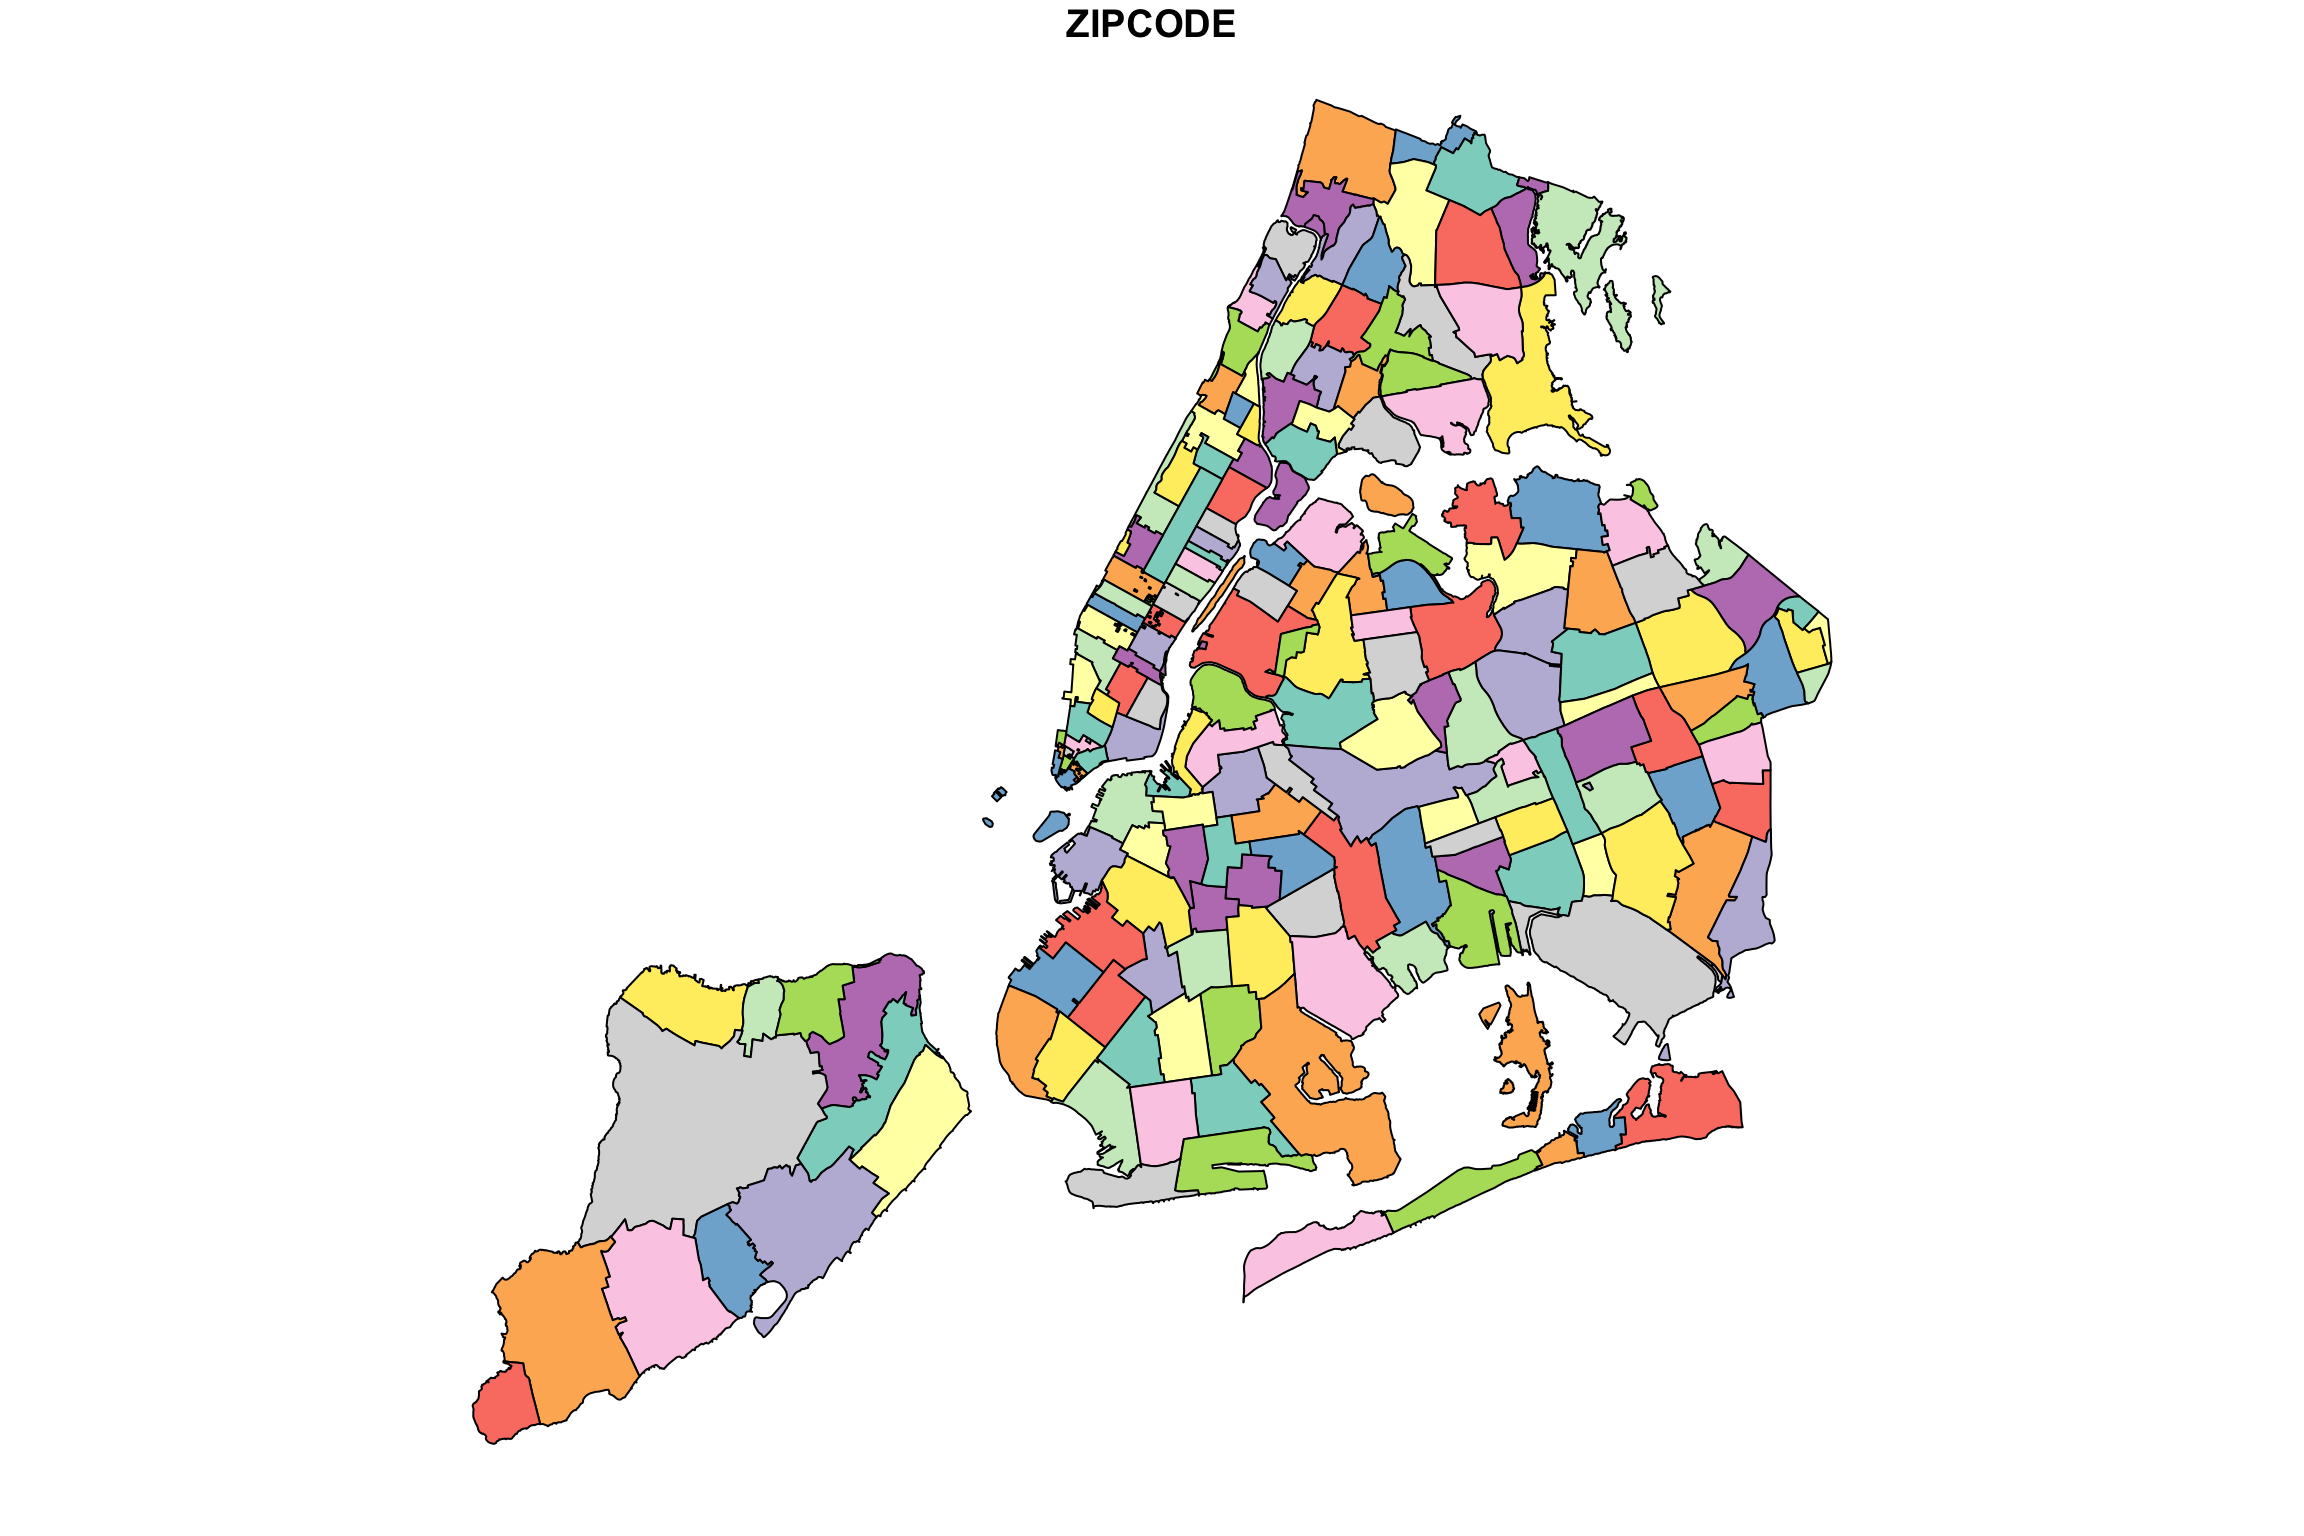
\includegraphics[width=0.9\linewidth]{carpedatum_files/figure-html/unnamed-chunk-81-1} \end{center}

Woot! There be zipcodes! Without any other data. Just boundaries and a candy-color palette to differentiate each area. If you are following along in an RStudio session, you can get a higher quality image by uncommenting the \texttt{quartz()} command. This will open the drawing in a new window. Note that it takes a little while to finish, and you can see it draw the boundaries of each zipcode one at a time\ldots{} aww!

To add specific colors or shades, we will need to send color/shade information along with the plot instruction\ldots{} but there's something else we need to do first.

How many zip codes are in our data set? The answer can be found by the number of rows in our data frame:

\begin{Shaded}
\begin{Highlighting}[]
\FunctionTok{nrow}\NormalTok{(zcta\_join)}
\end{Highlighting}
\end{Shaded}

\begin{verbatim}
## [1] 177
\end{verbatim}

Is this the same as the number of zip codes in our shapefile? If it isn't, then we will get issues when we combine the data we want to map with the geographic boundary data.

\begin{Shaded}
\begin{Highlighting}[]
\CommentTok{\#get zipcodes from shape file}
\NormalTok{shapezips }\OtherTok{\textless{}{-}}\NormalTok{ NYC\_zips}\SpecialCharTok{$}\NormalTok{ZIPCODE }
\FunctionTok{length}\NormalTok{(shapezips)}
\end{Highlighting}
\end{Shaded}

\begin{verbatim}
## [1] 263
\end{verbatim}

Not only are there more zipcodes in the shapefile than we have data for, but, for whatever reason involving the design of shapefiles, some zipcodes appear more than once. This is a small nuisance, but it can be solved by using \texttt{join} as before. The main idea is that we pass the data we have, and provide ``missing'' values (\texttt{NA} in R) for everything else.
Here is how to repackage our dataset to fit with the shapefile

\begin{Shaded}
\begin{Highlighting}[]
\CommentTok{\# start with one zipcode variable for everything in the shapefile}
\NormalTok{mapData }\OtherTok{\textless{}{-}} \FunctionTok{data.frame}\NormalTok{(}\AttributeTok{zipcode =}\NormalTok{ shapezips, }\AttributeTok{stringsAsFactors =} \ConstantTok{FALSE}\NormalTok{)}

\CommentTok{\# add the rest of our data to this}
\NormalTok{mapData }\OtherTok{\textless{}{-}} \FunctionTok{left\_join}\NormalTok{(mapData, zcta\_join, }\AttributeTok{by=}\FunctionTok{c}\NormalTok{(}\StringTok{"zipcode"}\NormalTok{))}
\end{Highlighting}
\end{Shaded}

Simple enough. We expected there to be zipcodes with missing census/COVID-19 data. Indeed, here are some:

\begin{Shaded}
\begin{Highlighting}[]
\FunctionTok{tail}\NormalTok{(mapData)}
\end{Highlighting}
\end{Shaded}

\begin{verbatim}
##     zipcode Median_HH_Income Median_Income zcta_propOver65 Total_Pop Median_Age
## 258   11414            71648         45640            22.0     29219       45.0
## 259   10310            72093         44590            13.4     23262       38.8
## 260   11693            59431         44674            12.3     12919       39.5
## 261   11249               NA            NA              NA        NA         NA
## 262   10162               NA            NA              NA        NA         NA
## 263   10119               NA            NA              NA        NA         NA
##     Median_Age_Male Median_Age_Fem Total_HispRace Hisp_Latin NH_Black NH_White
## 258            43.9           46.0          29219       22.3      1.8     67.8
## 259            38.2           39.1          23262       31.6     18.9     41.6
## 260            35.2           43.1          12919       29.5     16.1     46.9
## 261              NA             NA             NA         NA       NA       NA
## 262              NA             NA             NA         NA       NA       NA
## 263              NA             NA             NA         NA       NA       NA
##     NH_Asian NH_Other Bachelors Masters Professional Doctorate Total_EducPop
## 258      5.0      3.0      3828    1737          419        50         21607
## 259      6.2      1.7      2995    1768          409       150         15599
## 260      4.0      3.5      1401     828          114        10          8924
## 261       NA       NA        NA      NA           NA        NA            NA
## 262       NA       NA        NA      NA           NA        NA            NA
## 263       NA       NA        NA      NA           NA        NA            NA
##     HH1pers HH2pers HH3pers HH4plus Bach_plus_prop    AvgHH Positive Total
## 258    2603    3398    2151    2528           27.9 2.431086      588  1004
## 259    1971    2326    1628    2421           34.1 2.539061      506  1136
## 260    1469    1630     779     967           26.4 2.256760      256   444
## 261      NA      NA      NA      NA             NA       NA       NA    NA
## 262      NA      NA      NA      NA             NA       NA       NA    NA
## 263      NA      NA      NA      NA             NA       NA       NA    NA
##     zcta_cum.perc_pos
## 258             58.57
## 259             44.54
## 260             57.66
## 261                NA
## 262                NA
## 263                NA
\end{verbatim}

Why are these zipcodes (and others) missing data? It's hard to know, and you need to look at it case by case. Some of these are zipcodes for special areas, like industrial zones, airports. and train stations. (10119 appears to be Penn Station).

\hypertarget{coloring-in-the-shapes}{%
\subsection*{Coloring in the shapes}\label{coloring-in-the-shapes}}
\addcontentsline{toc}{subsection}{Coloring in the shapes}

So, suppose we want to color in the zip code boundaries to indicate the share of college educated adults in each region. We either have the college rate in our data frame, or we have the data needed to calculate it. (In this case, we might have total college and total population, so we can compute the case rate.)

But what is the right way to map case rate, which is a numeric/quantitative variable to color? What kind of variable is color? This is a profound question that has to do with perception through our sense. Questions regarding mental perception of sounds, colors, or short-duration verbal cues, for example, are the domain of \textbf{psychophysics} (yes, that's a real thing!)

Without delving too deeply into this problem, we can at least try to emulate the common practices in similar visualizations. What you'll see is that in many cases, rather than mapping a continuous range of values (e.g., COVID-19 case rate) to a continuous range of colors/shades, the values and the colors are discretized into a small number of levels. Each zip code area, then, is mapped to one of these levels and thus one of the corresponding colors/shades. In the media reports referenced early in this chapter, five levels was pretty typical.

\hypertarget{an-important-digression-on-choosing-your-levels}{%
\subsubsection*{An important digression on choosing your levels}\label{an-important-digression-on-choosing-your-levels}}
\addcontentsline{toc}{subsubsection}{An important digression on choosing your levels}

Let's say we want five levels. Sometimes the level-groupings of data are associated with quintiles. Recall that quintiles divide our ordered data set into five equally-sized partitions. Meaning, we will have the same number of zip codes in the lowest quintile, and the next lowest, and so on. But one could also make five partitions where the \emph{range of values is equally sized} but the number of cases in each partition is not. Think of the bin-breaks in a histogram. These are equally-sized ranges, but each bin does not necessarily have the same number of cases. Say, if the distribution is bell-shaped.

Here is an example using fake data, drawn in fact from a normal distribution:

\begin{Shaded}
\begin{Highlighting}[]
\CommentTok{\# make some data}
\NormalTok{someNormalData }\OtherTok{\textless{}{-}} \FunctionTok{rnorm}\NormalTok{(}\DecValTok{200}\NormalTok{, }\AttributeTok{mean=}\DecValTok{0}\NormalTok{, }\AttributeTok{sd =} \FloatTok{0.5}\NormalTok{)}

\CommentTok{\# slice it up into 5 groups, two ways:}
\NormalTok{quintileAssignments }\OtherTok{\textless{}{-}} \FunctionTok{ntile}\NormalTok{(someNormalData, }\AttributeTok{n=}\DecValTok{5}\NormalTok{)}
\NormalTok{partitionRanges }\OtherTok{\textless{}{-}} \FunctionTok{c}\NormalTok{(}\SpecialCharTok{{-}}\FloatTok{2.5}\NormalTok{,}\SpecialCharTok{{-}}\FloatTok{1.5}\NormalTok{,}\SpecialCharTok{{-}}\FloatTok{0.5}\NormalTok{, }\FloatTok{0.5}\NormalTok{, }\FloatTok{1.5}\NormalTok{,}\FloatTok{2.5}\NormalTok{)}
\NormalTok{equalRangeAssignments }\OtherTok{\textless{}{-}} \FunctionTok{cut}\NormalTok{(someNormalData, partitionRanges)}

\CommentTok{\# show how many cases are bucketed into each level}
\FunctionTok{table}\NormalTok{(quintileAssignments)}
\end{Highlighting}
\end{Shaded}

\begin{verbatim}
## quintileAssignments
##  1  2  3  4  5 
## 40 40 40 40 40
\end{verbatim}

\begin{Shaded}
\begin{Highlighting}[]
\FunctionTok{table}\NormalTok{(equalRangeAssignments)}
\end{Highlighting}
\end{Shaded}

\begin{verbatim}
## equalRangeAssignments
## (-2.5,-1.5] (-1.5,-0.5]  (-0.5,0.5]   (0.5,1.5]   (1.5,2.5] 
##           1          28         142          29           0
\end{verbatim}

As you can see, the number of cases that get collected in these buckets can be different, depending on how we slice it. If we were mapping zipcodes to colors based on the values of some data such as these, then we would get very different maps. In the quantile case (quintiles, specifically!), we would have our colors spread out, or varying, more. In the equal range case, we may have only a few extreme colors, while the majority of the zipcodes are the same color. All of this happened because our data distribution was bell-shaped. Admittedly, if the distribution were flat (also known as a uniform distribution), then both methods would divide the cases similarly.

By the way, to see what the actual ranges of the quintiles are (this depends on the data you have), you can do this:

\begin{Shaded}
\begin{Highlighting}[]
\FunctionTok{quantile}\NormalTok{(someNormalData, }\AttributeTok{probs =} \FunctionTok{seq}\NormalTok{(}\DecValTok{0}\NormalTok{, }\DecValTok{1}\NormalTok{, }\AttributeTok{length.out=}\DecValTok{6}\NormalTok{)) }\SpecialCharTok{\%\textgreater{}\%} 
  \FunctionTok{cut}\NormalTok{(someNormalData, .) }\SpecialCharTok{\%\textgreater{}\%}\NormalTok{ levels}
\end{Highlighting}
\end{Shaded}

\begin{verbatim}
## [1] "(-1.56,-0.387]"   "(-0.387,-0.0771]" "(-0.0771,0.138]"  "(0.138,0.417]"   
## [5] "(0.417,1.39]"
\end{verbatim}

This ends the digression. The reason it is important is that this choice of how to make your level assignments will ultimately change how the map looks, and thus what it communicates. We will have a chance to see this play out next.

\hypertarget{college}{%
\subsubsection*{College}\label{college}}
\addcontentsline{toc}{subsubsection}{College}

We already have a variable called ``Bach\_plus\_prop'' which accounts for the proportion of college among adults 25 and over. Let's see how this actual data set can get mapped. Because this has already gotten complicated enough, I've wrapped a couple of steps together into a function called \texttt{getShapeColors}. Feel free to simply ignore this if you already have enough on your mind and just skip to the example of how to use it.

\begin{Shaded}
\begin{Highlighting}[]
\CommentTok{\# Safe to ignore this chunk}
\NormalTok{getShapeColors }\OtherTok{\textless{}{-}} \ControlFlowTok{function}\NormalTok{(data, }\AttributeTok{nbreaks=}\DecValTok{5}\NormalTok{, }\AttributeTok{missingcol=}\StringTok{"gray88"}\NormalTok{, }
                           \AttributeTok{rdgrbl=}\FunctionTok{c}\NormalTok{(}\DecValTok{0}\NormalTok{,}\DecValTok{0}\NormalTok{,}\DecValTok{1}\NormalTok{), }\AttributeTok{mycolors=}\ConstantTok{NULL}\NormalTok{)\{}
  \ControlFlowTok{if}\NormalTok{(}\FunctionTok{length}\NormalTok{(nbreaks) }\SpecialCharTok{==} \DecValTok{1}\NormalTok{) \{}
\NormalTok{    mybreaks }\OtherTok{\textless{}{-}} \FunctionTok{c}\NormalTok{(}\SpecialCharTok{{-}}\DecValTok{1}\NormalTok{, }\FunctionTok{quantile}\NormalTok{(data,}
                               \AttributeTok{probs =} \FunctionTok{seq}\NormalTok{(}\DecValTok{0}\NormalTok{, }\DecValTok{1}\NormalTok{, }\AttributeTok{length.out=}\NormalTok{nbreaks}\SpecialCharTok{+}\DecValTok{1}\NormalTok{),}
                               \AttributeTok{na.rm =}\NormalTok{ T))}
\NormalTok{  \} }\ControlFlowTok{else}\NormalTok{ \{}
\NormalTok{    mybreaks }\OtherTok{\textless{}{-}} \FunctionTok{c}\NormalTok{(}\SpecialCharTok{{-}}\DecValTok{1}\NormalTok{,nbreaks)}
\NormalTok{  \}}
  \ControlFlowTok{if}\NormalTok{(}\SpecialCharTok{!}\FunctionTok{is.null}\NormalTok{(mycolors))\{}
\NormalTok{    mycols }\OtherTok{\textless{}{-}}\NormalTok{ mycolors}
\NormalTok{  \} }\ControlFlowTok{else}\NormalTok{ \{}
\NormalTok{    mycols }\OtherTok{\textless{}{-}} \FunctionTok{rgb}\NormalTok{(rdgrbl[}\DecValTok{1}\NormalTok{],rdgrbl[}\DecValTok{2}\NormalTok{],rdgrbl[}\DecValTok{3}\NormalTok{],}
                  \FunctionTok{seq}\NormalTok{(}\FloatTok{0.05}\NormalTok{,}\FloatTok{0.65}\NormalTok{, }\AttributeTok{length.out =} \FunctionTok{length}\NormalTok{(mybreaks)}\SpecialCharTok{{-}}\DecValTok{1}\NormalTok{))}
\NormalTok{  \}}
\NormalTok{  mycols[}\DecValTok{1}\NormalTok{] }\OtherTok{\textless{}{-}}\NormalTok{ missingcol}
\NormalTok{  data[}\FunctionTok{is.na}\NormalTok{(data)] }\OtherTok{\textless{}{-}} \SpecialCharTok{{-}}\NormalTok{.}\DecValTok{1}
\NormalTok{  mycolorscheme }\OtherTok{\textless{}{-}} \FunctionTok{cut}\NormalTok{(data, mybreaks) }\SpecialCharTok{\%\textgreater{}\%}
    \FunctionTok{as.numeric}\NormalTok{()}
\NormalTok{  mycolorscheme }\OtherTok{\textless{}{-}}\NormalTok{ mycols[mycolorscheme]}
\NormalTok{  levs }\OtherTok{\textless{}{-}} \FunctionTok{levels}\NormalTok{(}\FunctionTok{cut}\NormalTok{(data, mybreaks))}
\NormalTok{  levs[}\DecValTok{1}\NormalTok{] }\OtherTok{\textless{}{-}} \StringTok{"No Data"}
  \FunctionTok{return}\NormalTok{(}\FunctionTok{list}\NormalTok{(}\AttributeTok{regionValues=}\NormalTok{mycolorscheme, }
              \AttributeTok{legendText=}\NormalTok{levs, }
              \AttributeTok{legendColors=}\NormalTok{mycols))}
\NormalTok{\}}
\end{Highlighting}
\end{Shaded}

Here's how you use it:

\begin{Shaded}
\begin{Highlighting}[]
\NormalTok{bachelorPlus }\OtherTok{\textless{}{-}}\NormalTok{ mapData}\SpecialCharTok{$}\NormalTok{Bach\_plus\_prop}
\NormalTok{myShapeColors }\OtherTok{\textless{}{-}} \FunctionTok{getShapeColors}\NormalTok{(bachelorPlus, }\AttributeTok{nbreaks=}\DecValTok{5}\NormalTok{)}

\FunctionTok{plot}\NormalTok{(NYC\_zips[,}\DecValTok{1}\NormalTok{], }\AttributeTok{col =}\NormalTok{ myShapeColors}\SpecialCharTok{$}\NormalTok{regionValues, }
     \AttributeTok{main =} \StringTok{"Share of Adults with College Degree"}\NormalTok{, }
     \AttributeTok{cex =} \DecValTok{10}\NormalTok{, }\AttributeTok{lwd=}\FloatTok{0.05}\NormalTok{)}
\FunctionTok{legend}\NormalTok{(}\StringTok{"topleft"}\NormalTok{, }
       \AttributeTok{legend =}\NormalTok{ myShapeColors}\SpecialCharTok{$}\NormalTok{legendText, }
       \AttributeTok{fill =}\NormalTok{ myShapeColors}\SpecialCharTok{$}\NormalTok{legendColors, }\AttributeTok{cex =} \FloatTok{0.8}\NormalTok{, }
       \AttributeTok{title =} \StringTok{"College Prop"}\NormalTok{)}
\end{Highlighting}
\end{Shaded}

\begin{center}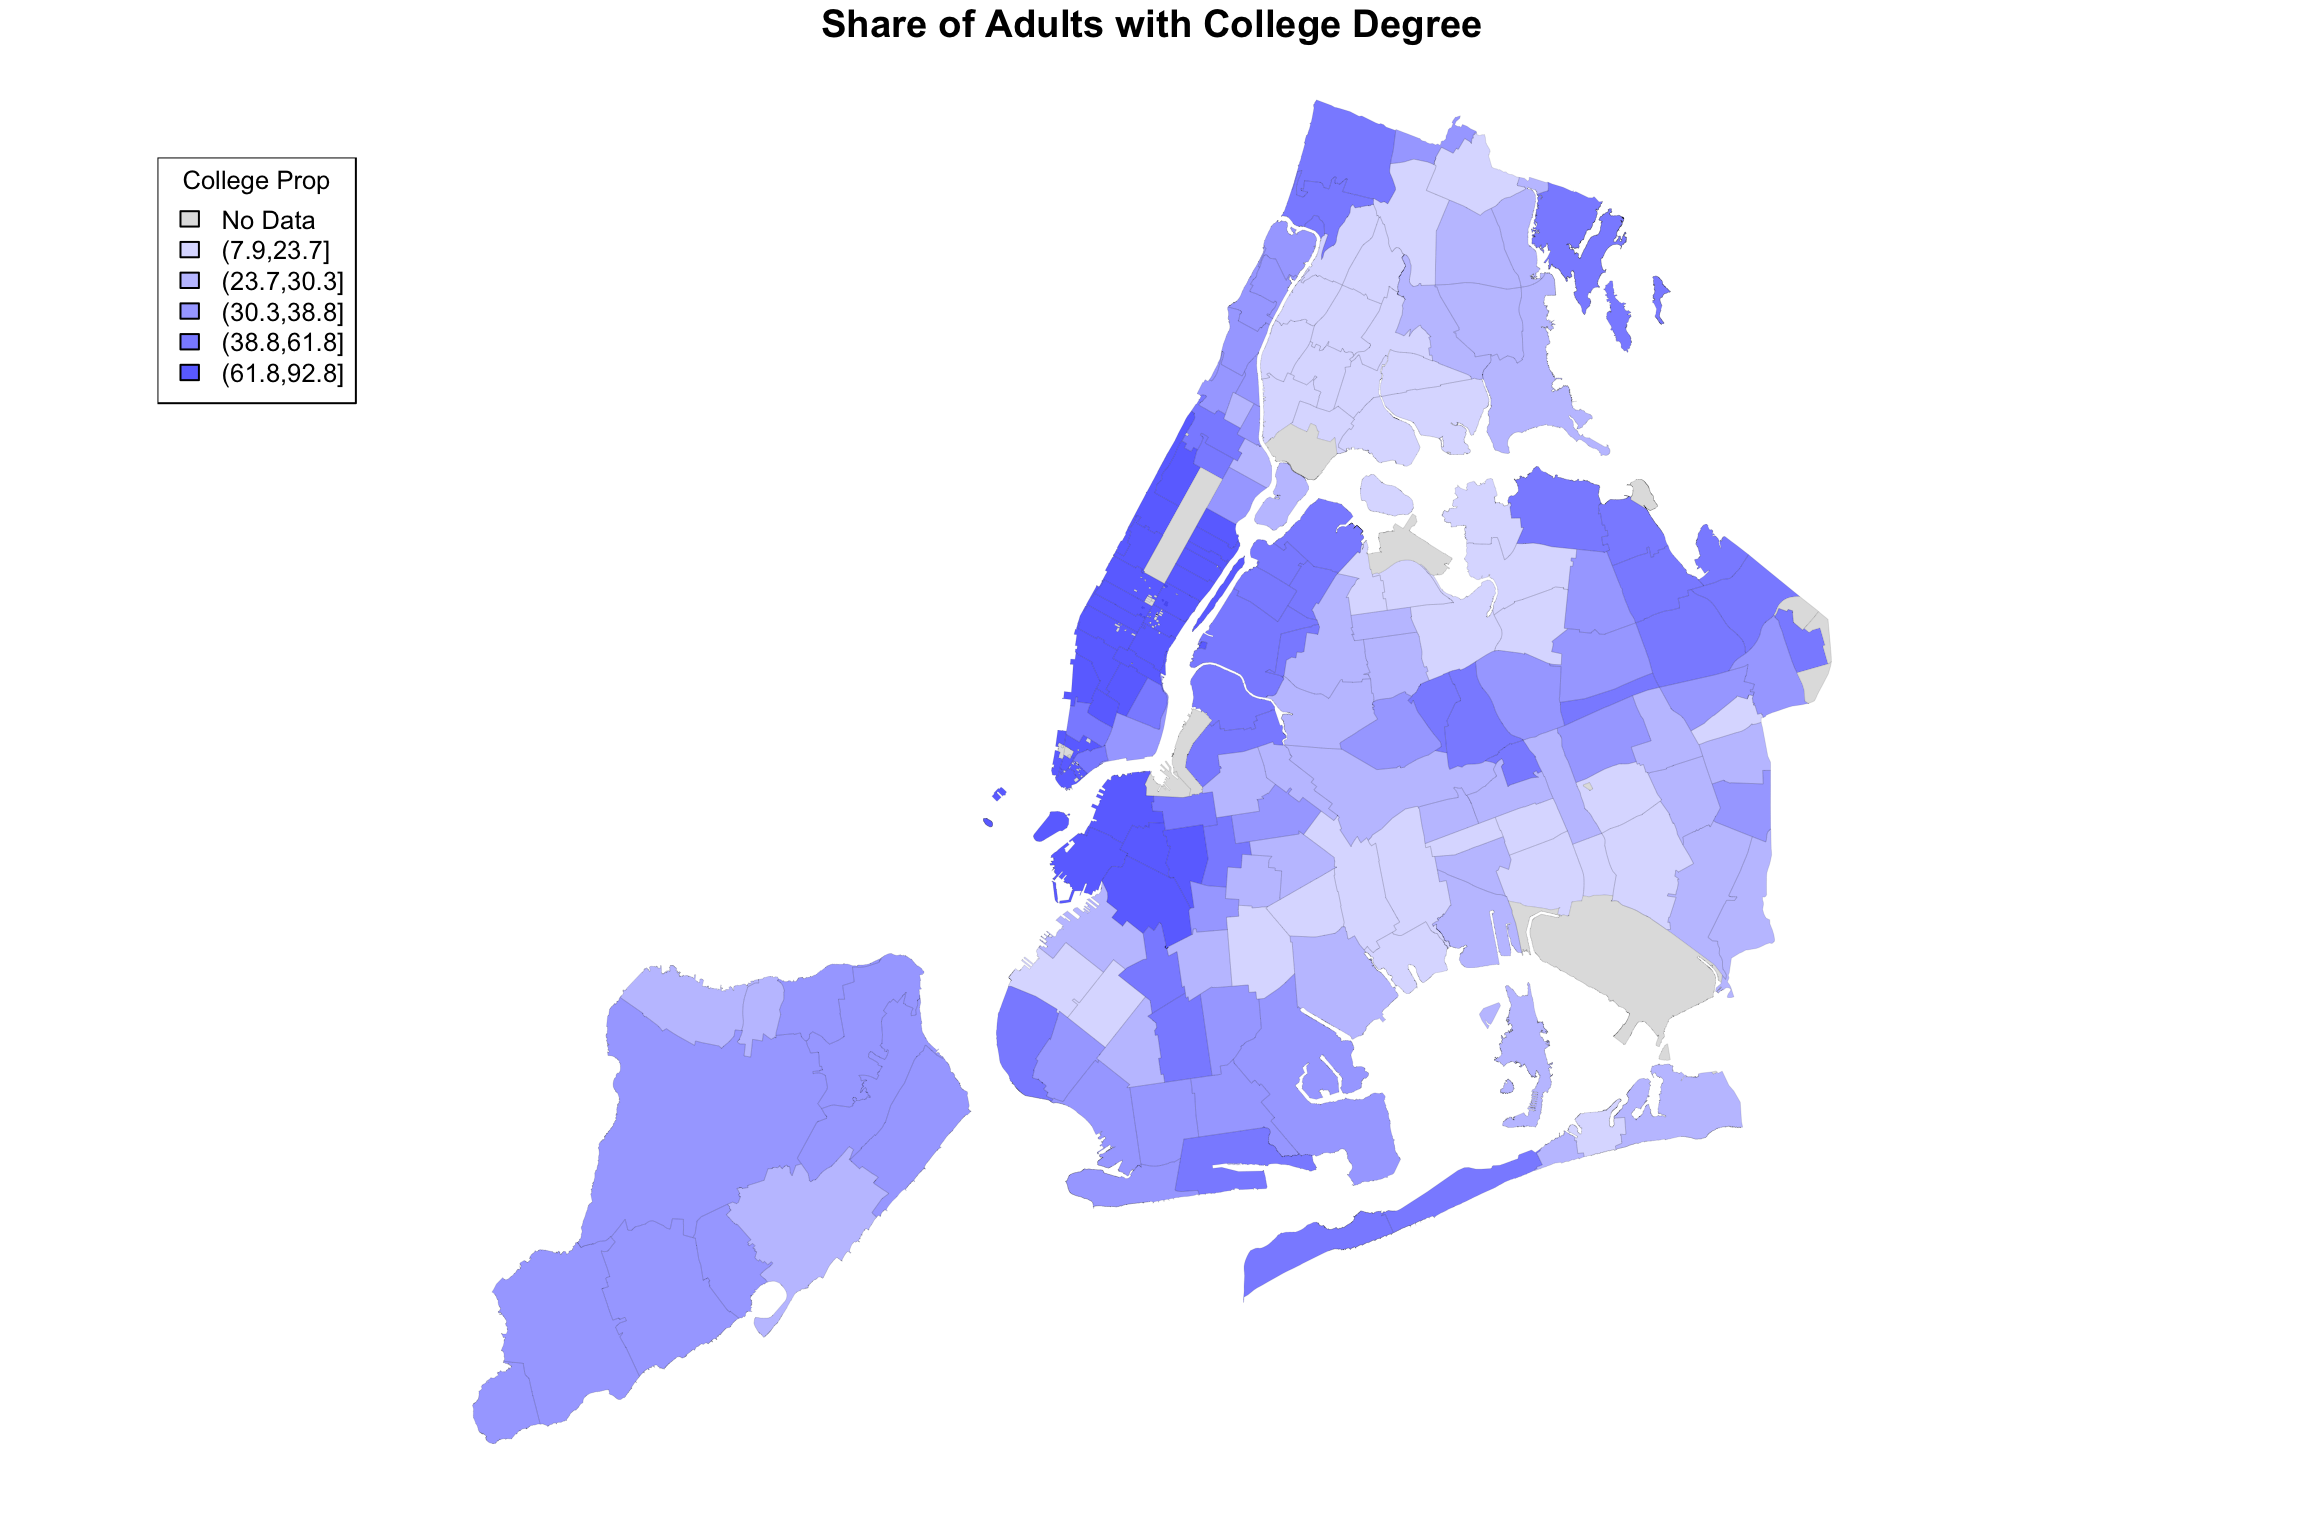
\includegraphics[width=0.9\linewidth]{carpedatum_files/figure-html/unnamed-chunk-89-1} \end{center}

Hallelujah, we finally have made an image of something. Notice that the output of the \texttt{getShapeColors} functions contains three elements (it is technically a list): values (colors values for each geographic area), legend (text for the legend, including the ranges of values), and palette (these are the colors that go into the len).

The input of \texttt{getShapeColors} is the data you want to visualize as well as the number of levels. In this example, we chose 5. By default, the color palette is shades of blue, but as it is written, you can provide different colors if you like. For example, the Furman report used a color palette called viridis, which ranges from dark blue to yellow. The only modification necessary is to add an argument to the function:

\begin{Shaded}
\begin{Highlighting}[]
\NormalTok{myShapeColors }\OtherTok{\textless{}{-}} \FunctionTok{getShapeColors}\NormalTok{(bachelorPlus, }\AttributeTok{nbreaks=}\DecValTok{5}\NormalTok{, }\AttributeTok{mycolors=}\FunctionTok{viridis}\NormalTok{(}\DecValTok{6}\NormalTok{))}

\FunctionTok{plot}\NormalTok{(NYC\_zips[,}\DecValTok{1}\NormalTok{], }\AttributeTok{col =}\NormalTok{ myShapeColors}\SpecialCharTok{$}\NormalTok{regionValues, }
     \AttributeTok{main =} \StringTok{"Share of Adults with College Degree"}\NormalTok{, }\AttributeTok{cex =} \DecValTok{10}\NormalTok{, }\AttributeTok{lwd=}\FloatTok{0.05}\NormalTok{)}
\FunctionTok{legend}\NormalTok{(}\StringTok{"topleft"}\NormalTok{, }
       \AttributeTok{legend =}\NormalTok{ myShapeColors}\SpecialCharTok{$}\NormalTok{legendText, }
       \AttributeTok{fill =}\NormalTok{ myShapeColors}\SpecialCharTok{$}\NormalTok{legendColors, }\AttributeTok{cex =} \FloatTok{0.8}\NormalTok{, }\AttributeTok{title =} \StringTok{"College Prop"}\NormalTok{)}
\end{Highlighting}
\end{Shaded}

\begin{center}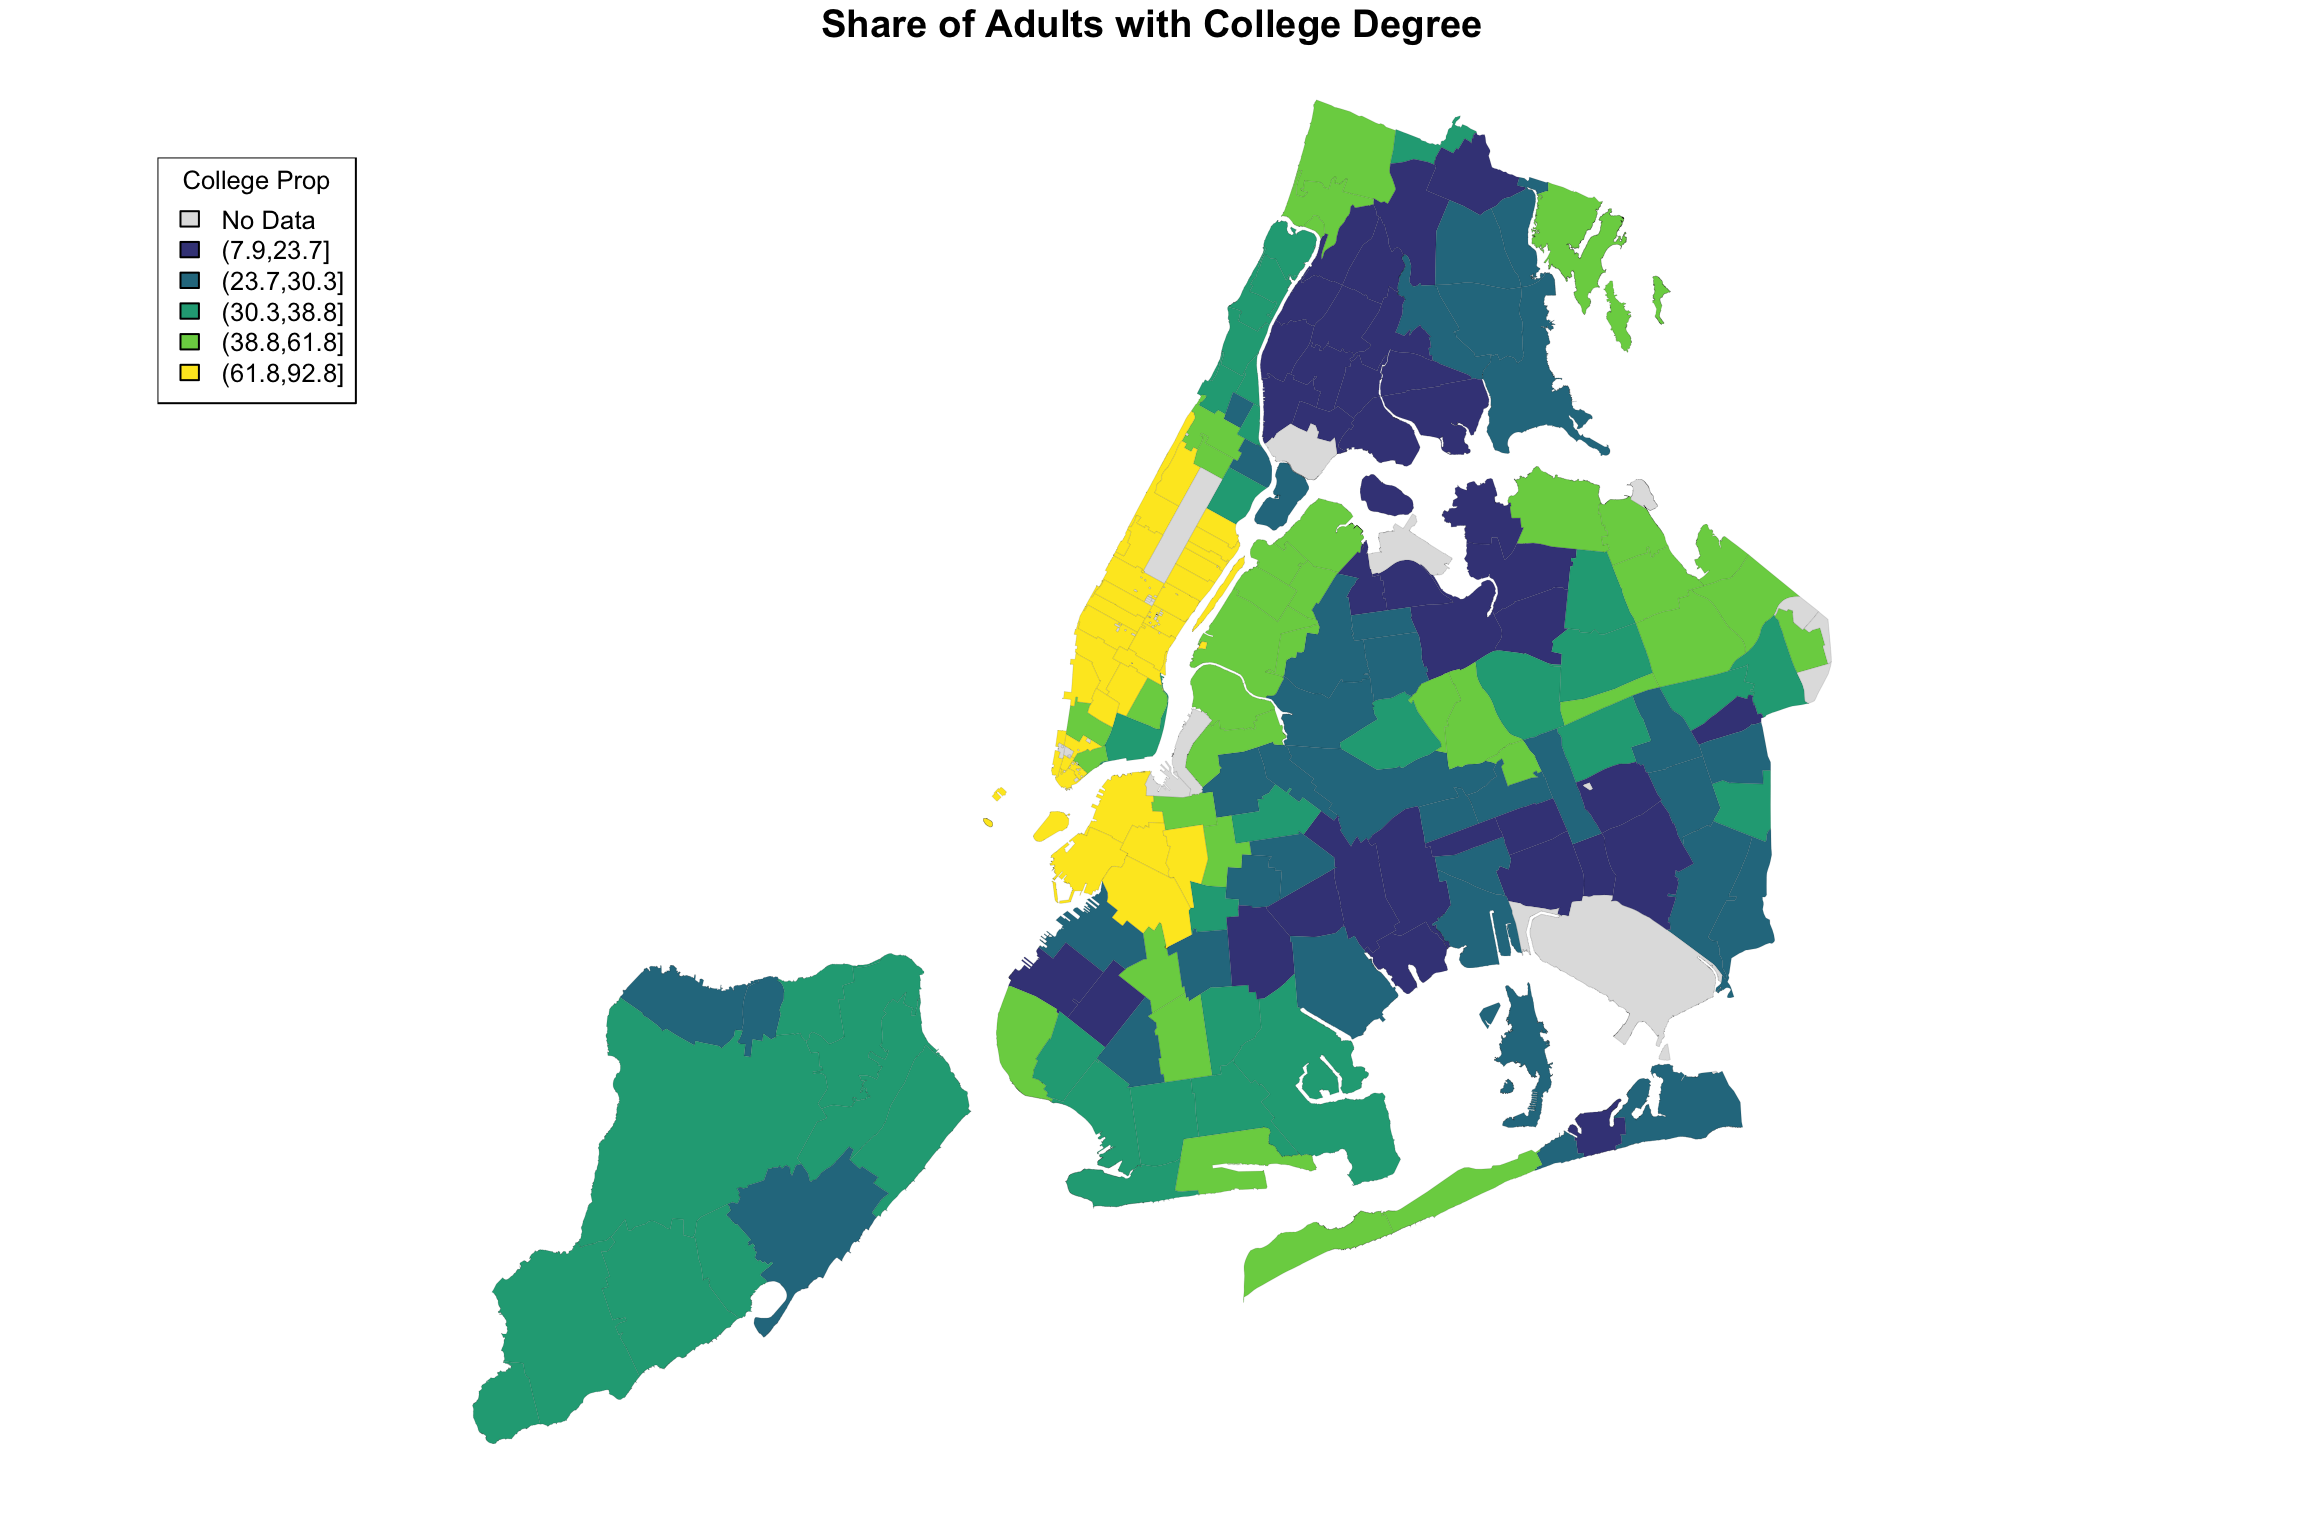
\includegraphics[width=0.9\linewidth]{carpedatum_files/figure-html/unnamed-chunk-90-1} \end{center}

I don't know exactly how ABCNews made their color palette, but here is my approximation. I played around with the border color and line width as well.

\begin{Shaded}
\begin{Highlighting}[]
\NormalTok{ABCpalette }\OtherTok{\textless{}{-}} \FunctionTok{c}\NormalTok{(}\StringTok{"gray88"}\NormalTok{, }\StringTok{"\#4e9ccb"}\NormalTok{, }\StringTok{"\#3b7ba9"}\NormalTok{,}\StringTok{"\#265982"}\NormalTok{, }\StringTok{"\#133960"}\NormalTok{,}\StringTok{"\#001a3a"}\NormalTok{)}
\NormalTok{myShapeColors }\OtherTok{\textless{}{-}} \FunctionTok{getShapeColors}\NormalTok{(bachelorPlus, }\AttributeTok{nbreaks=}\DecValTok{5}\NormalTok{, }\AttributeTok{mycolors=}\NormalTok{ABCpalette)}

\FunctionTok{plot}\NormalTok{(NYC\_zips[,}\DecValTok{1}\NormalTok{], }\AttributeTok{col =}\NormalTok{ myShapeColors}\SpecialCharTok{$}\NormalTok{regionValues, }
     \AttributeTok{main =} \StringTok{"Share of Adults with College Degree"}\NormalTok{, }
     \AttributeTok{cex =} \DecValTok{10}\NormalTok{, }\AttributeTok{border=}\StringTok{"white"}\NormalTok{, }\AttributeTok{lwd=}\FloatTok{0.25}\NormalTok{)}
\FunctionTok{legend}\NormalTok{(}\StringTok{"topleft"}\NormalTok{, }
       \AttributeTok{legend =}\NormalTok{ myShapeColors}\SpecialCharTok{$}\NormalTok{legendText, }
       \AttributeTok{fill =}\NormalTok{ myShapeColors}\SpecialCharTok{$}\NormalTok{legendColors, }\AttributeTok{cex =} \FloatTok{0.8}\NormalTok{, }\AttributeTok{title =} \StringTok{"College Share"}\NormalTok{)}
\end{Highlighting}
\end{Shaded}

\begin{center}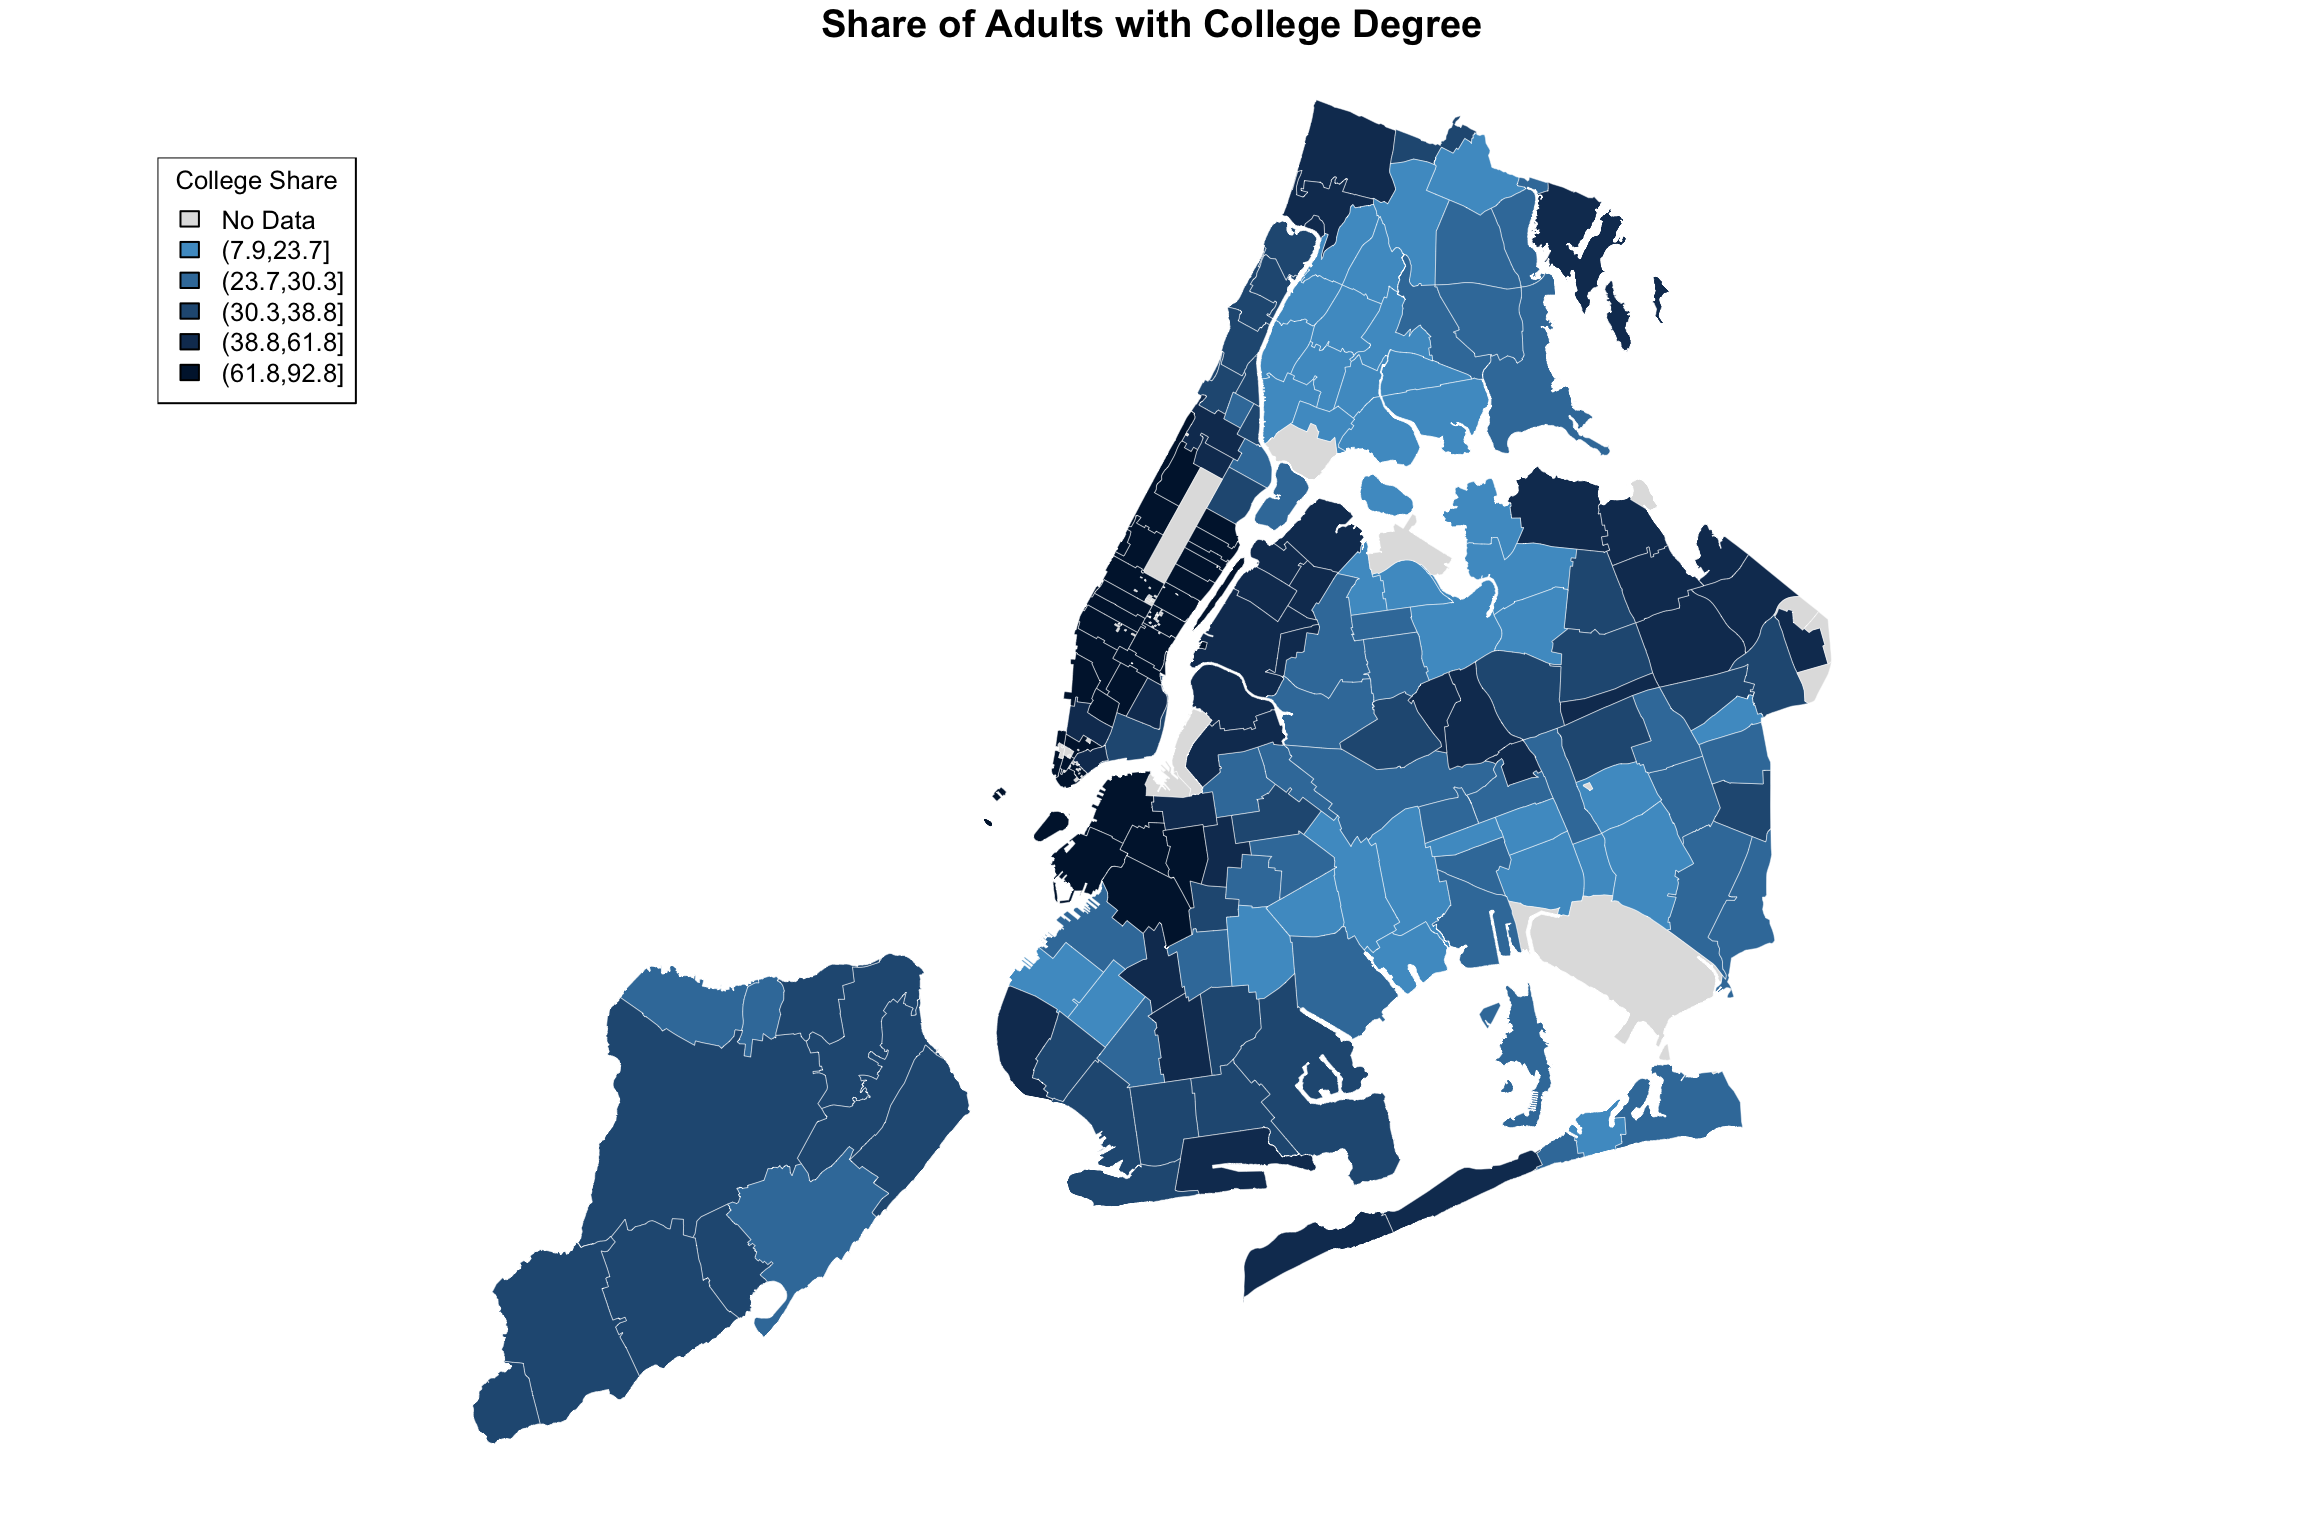
\includegraphics[width=0.9\linewidth]{carpedatum_files/figure-html/unnamed-chunk-91-1} \end{center}

Here is the original again.

\begin{figure}

{\centering 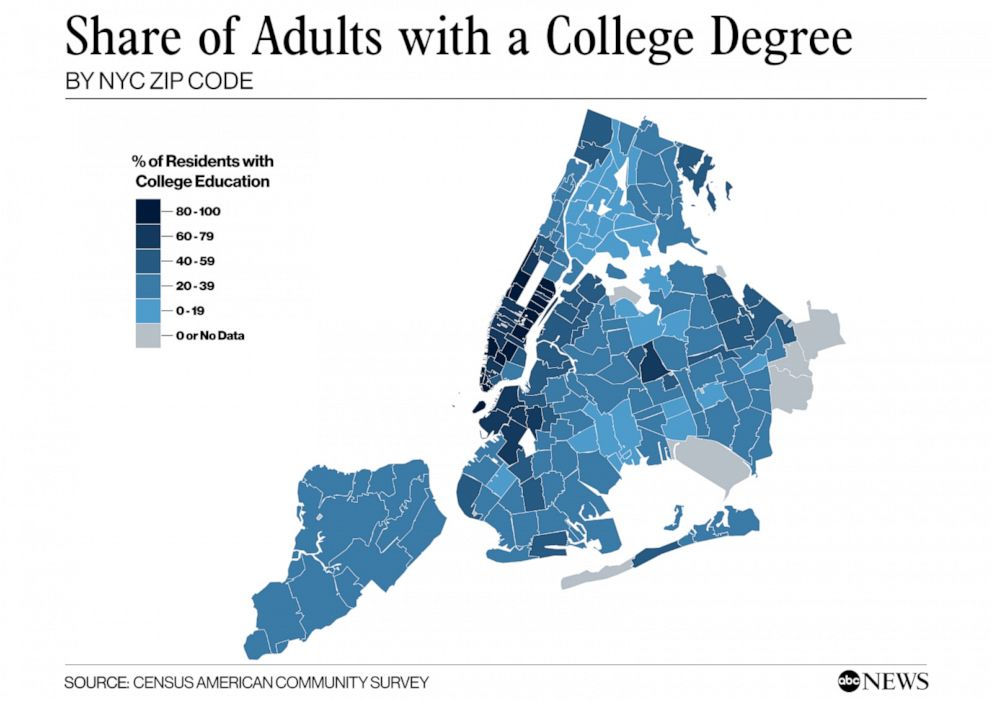
\includegraphics[width=0.8\linewidth]{images/abc_CollegeDegreeNycZip_v02_KA_hpEmbed_17x12_992} 

}

\caption{ABCNews visualization}\label{fig:abc-college}
\end{figure}

I hope you agree that it's pretty close! Did you spot the main difference? Sure, there are a few of them, but notice the legend in the ABCNews figure? ABCNews used fixed ranges for their level cutoffs, whereas we were using quintiles! What if we want custom cut-points that are not quantiles?

I anticipated this desire in the getShapeColors function, so it's easy enough. Instead of providing a number (e.g, 5) for \texttt{nbreaks}, you provide the actual list of cutpoints. Here it is on its own.

\begin{Shaded}
\begin{Highlighting}[]
\NormalTok{ABCpalette }\OtherTok{\textless{}{-}} \FunctionTok{c}\NormalTok{(}\StringTok{"gray88"}\NormalTok{, }\StringTok{"\#4e9ccb"}\NormalTok{, }\StringTok{"\#3b7ba9"}\NormalTok{,}\StringTok{"\#265982"}\NormalTok{, }\StringTok{"\#133960"}\NormalTok{,}\StringTok{"\#001a3a"}\NormalTok{)}
\NormalTok{myShapeColors }\OtherTok{\textless{}{-}} \FunctionTok{getShapeColors}\NormalTok{(bachelorPlus, }\AttributeTok{nbreaks=}\FunctionTok{c}\NormalTok{(}\DecValTok{0}\NormalTok{,}\DecValTok{20}\NormalTok{,}\DecValTok{40}\NormalTok{,}\DecValTok{60}\NormalTok{,}\DecValTok{80}\NormalTok{,}\DecValTok{100}\NormalTok{),}
                                 \AttributeTok{mycolors=}\NormalTok{ABCpalette)}

\FunctionTok{plot}\NormalTok{(NYC\_zips[,}\DecValTok{1}\NormalTok{], }\AttributeTok{col =}\NormalTok{ myShapeColors}\SpecialCharTok{$}\NormalTok{regionValues, }
     \AttributeTok{main =} \StringTok{"Share of Adults with College Degree"}\NormalTok{, }
     \AttributeTok{cex =} \DecValTok{10}\NormalTok{, }\AttributeTok{border=}\StringTok{"white"}\NormalTok{, }\AttributeTok{lwd=}\FloatTok{0.25}\NormalTok{)}
\FunctionTok{legend}\NormalTok{(}\StringTok{"topleft"}\NormalTok{, }
       \AttributeTok{legend =}\NormalTok{ myShapeColors}\SpecialCharTok{$}\NormalTok{legendText, }
       \AttributeTok{fill =}\NormalTok{ myShapeColors}\SpecialCharTok{$}\NormalTok{legendColors, }\AttributeTok{cex =} \FloatTok{0.8}\NormalTok{, }\AttributeTok{title =} \StringTok{"College Share"}\NormalTok{)}
\end{Highlighting}
\end{Shaded}

\begin{center}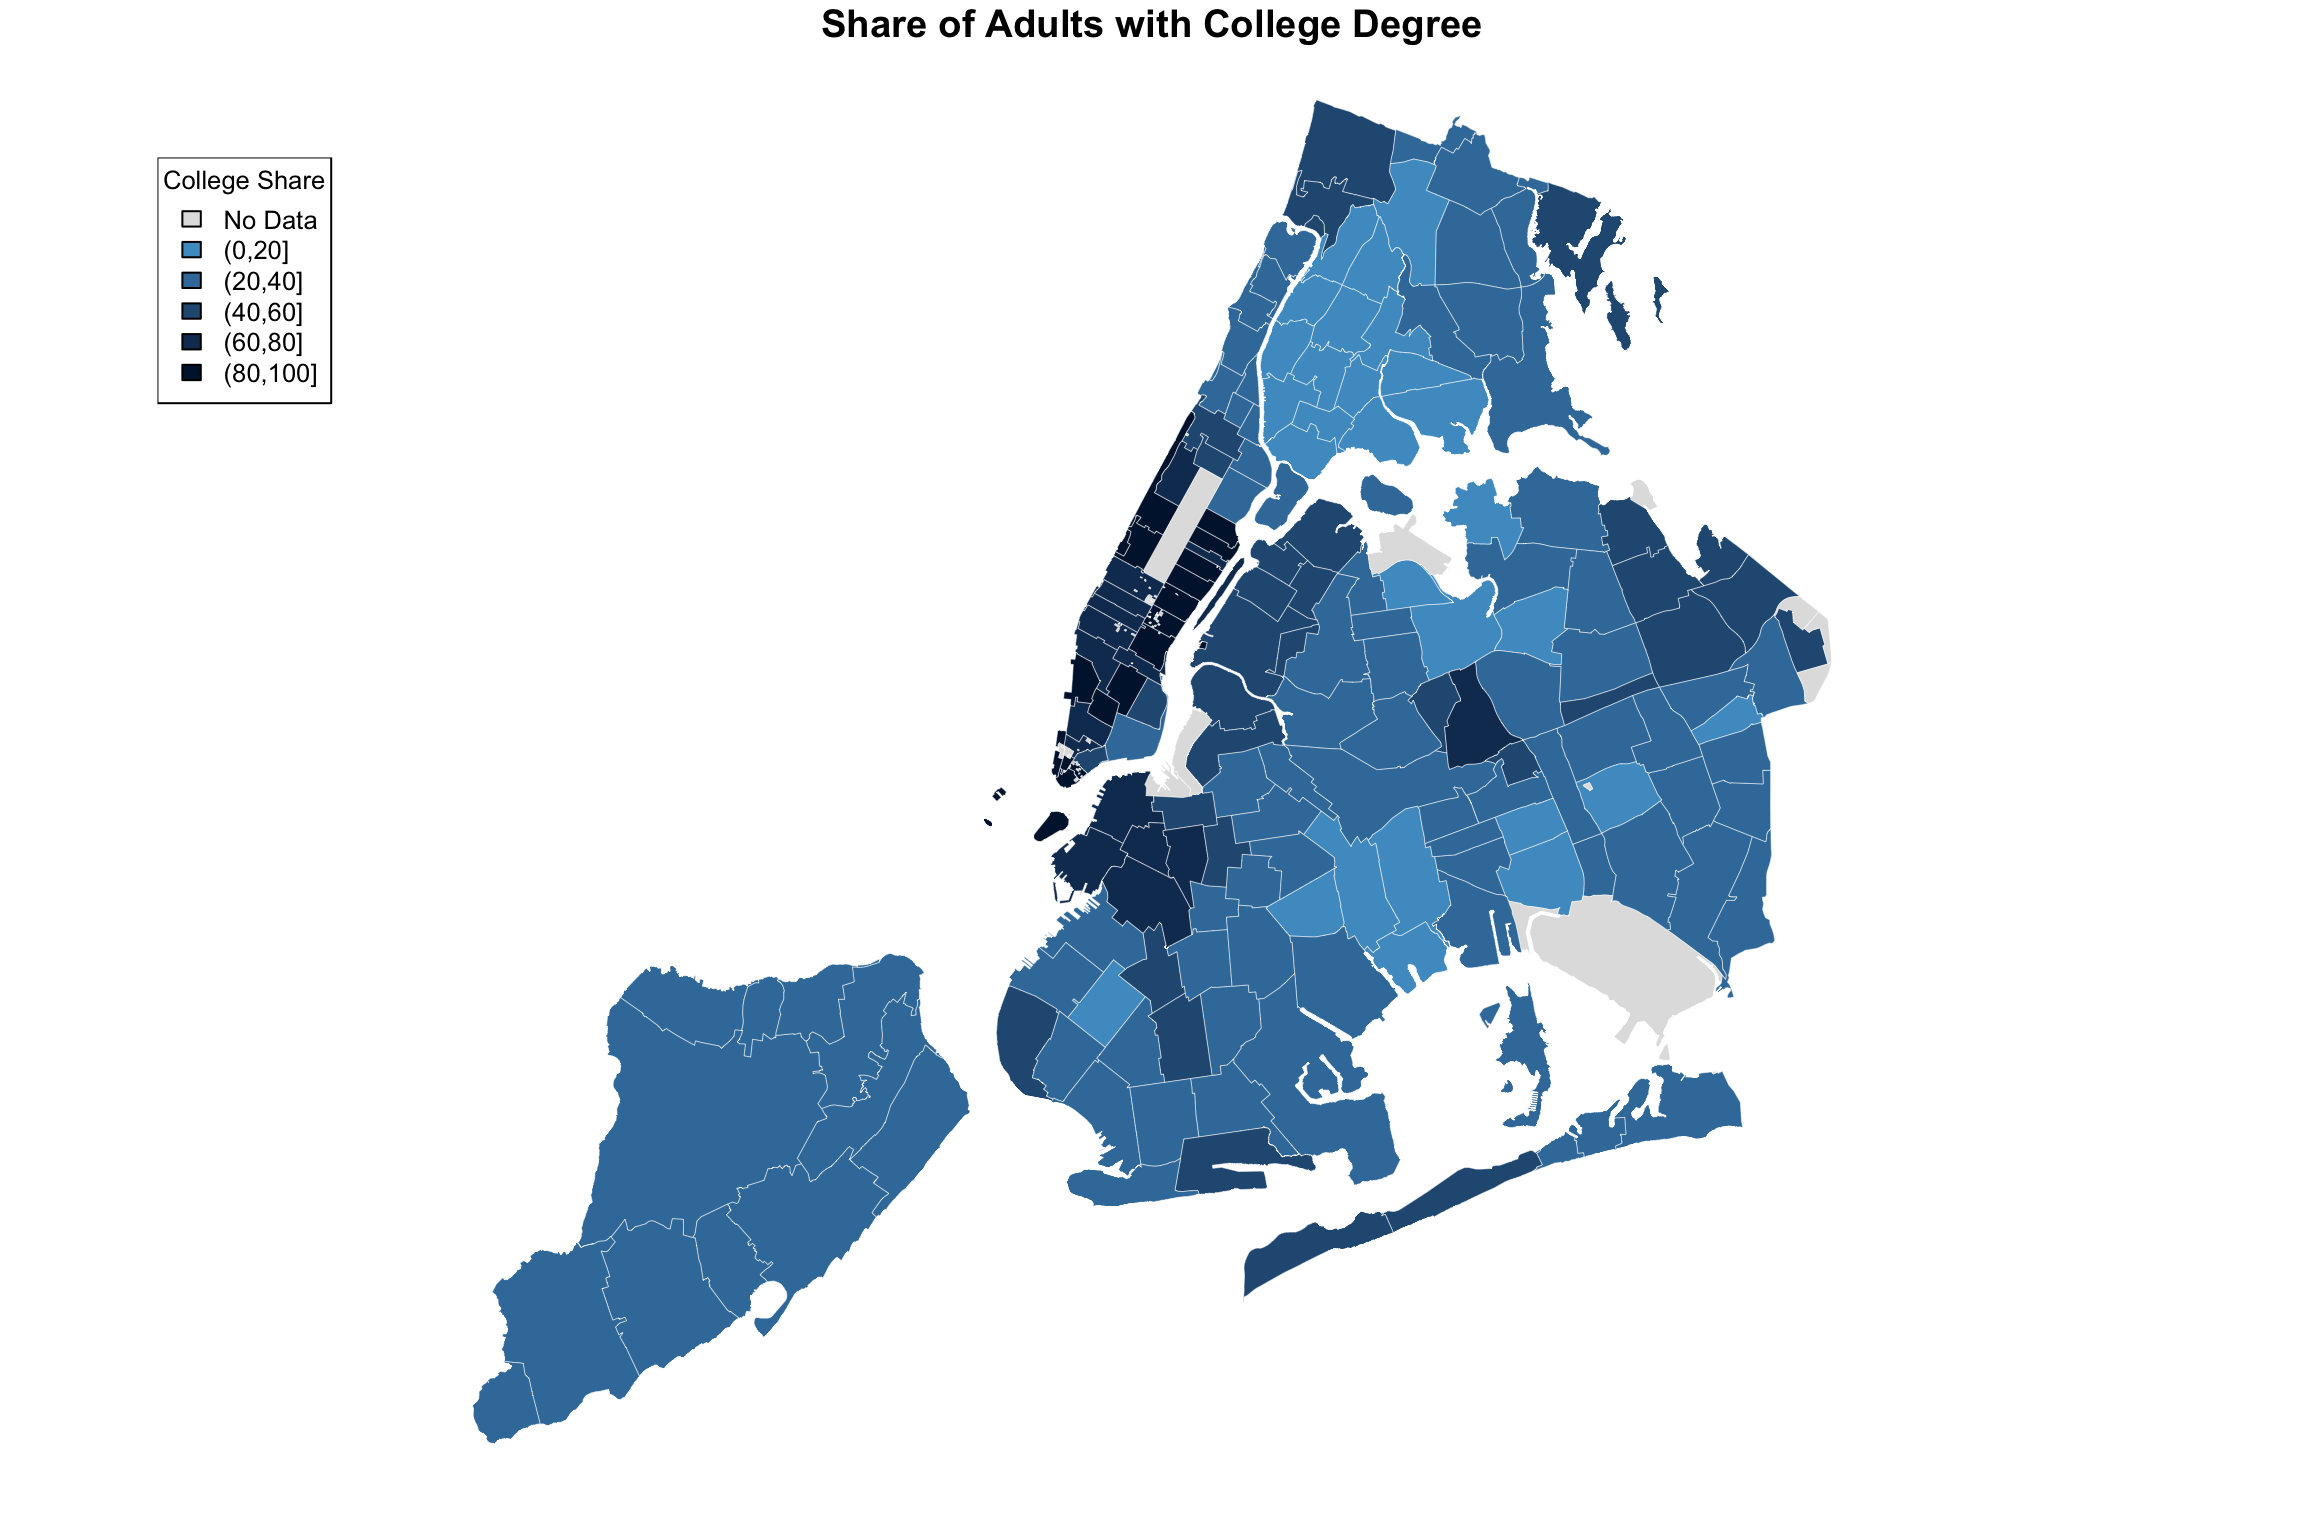
\includegraphics[width=0.9\linewidth]{carpedatum_files/figure-html/unnamed-chunk-92-1} \end{center}

And here are two versions of the same data, mapped side-by-side using different cut-points:

\begin{Shaded}
\begin{Highlighting}[]
\NormalTok{ABCpalette }\OtherTok{\textless{}{-}} \FunctionTok{c}\NormalTok{(}\StringTok{"gray88"}\NormalTok{, }\StringTok{"\#4e9ccb"}\NormalTok{, }\StringTok{"\#3b7ba9"}\NormalTok{,}\StringTok{"\#265982"}\NormalTok{, }\StringTok{"\#133960"}\NormalTok{,}\StringTok{"\#001a3a"}\NormalTok{)}
\NormalTok{myShapeColors1 }\OtherTok{\textless{}{-}} \FunctionTok{getShapeColors}\NormalTok{(bachelorPlus, }\AttributeTok{nbreaks=}\DecValTok{5}\NormalTok{,}
                                 \AttributeTok{mycolors=}\NormalTok{ABCpalette)}
\NormalTok{myShapeColors2 }\OtherTok{\textless{}{-}} \FunctionTok{getShapeColors}\NormalTok{(bachelorPlus, }\AttributeTok{nbreaks=}\FunctionTok{c}\NormalTok{(}\DecValTok{0}\NormalTok{,}\DecValTok{20}\NormalTok{,}\DecValTok{40}\NormalTok{,}\DecValTok{60}\NormalTok{,}\DecValTok{80}\NormalTok{,}\DecValTok{100}\NormalTok{),}
                                 \AttributeTok{mycolors=}\NormalTok{ABCpalette)}

\FunctionTok{par}\NormalTok{(}\AttributeTok{mfrow=}\FunctionTok{c}\NormalTok{(}\DecValTok{1}\NormalTok{,}\DecValTok{2}\NormalTok{))}

\FunctionTok{plot}\NormalTok{(NYC\_zips[,}\DecValTok{1}\NormalTok{], }\AttributeTok{col =}\NormalTok{ myShapeColors1}\SpecialCharTok{$}\NormalTok{regionValues, }
     \AttributeTok{main =} \StringTok{"\%College using Quintiles"}\NormalTok{, }
     \AttributeTok{cex =} \DecValTok{10}\NormalTok{, }\AttributeTok{border=}\StringTok{"white"}\NormalTok{, }\AttributeTok{lwd=}\FloatTok{0.25}\NormalTok{)}
\FunctionTok{legend}\NormalTok{(}\StringTok{"topleft"}\NormalTok{, }
       \AttributeTok{legend =}\NormalTok{ myShapeColors1}\SpecialCharTok{$}\NormalTok{legendText, }
       \AttributeTok{fill =}\NormalTok{ myShapeColors1}\SpecialCharTok{$}\NormalTok{legendColors, }\AttributeTok{cex =} \FloatTok{0.8}\NormalTok{, }\AttributeTok{title =} \StringTok{"College Share"}\NormalTok{)}
\end{Highlighting}
\end{Shaded}

\begin{center}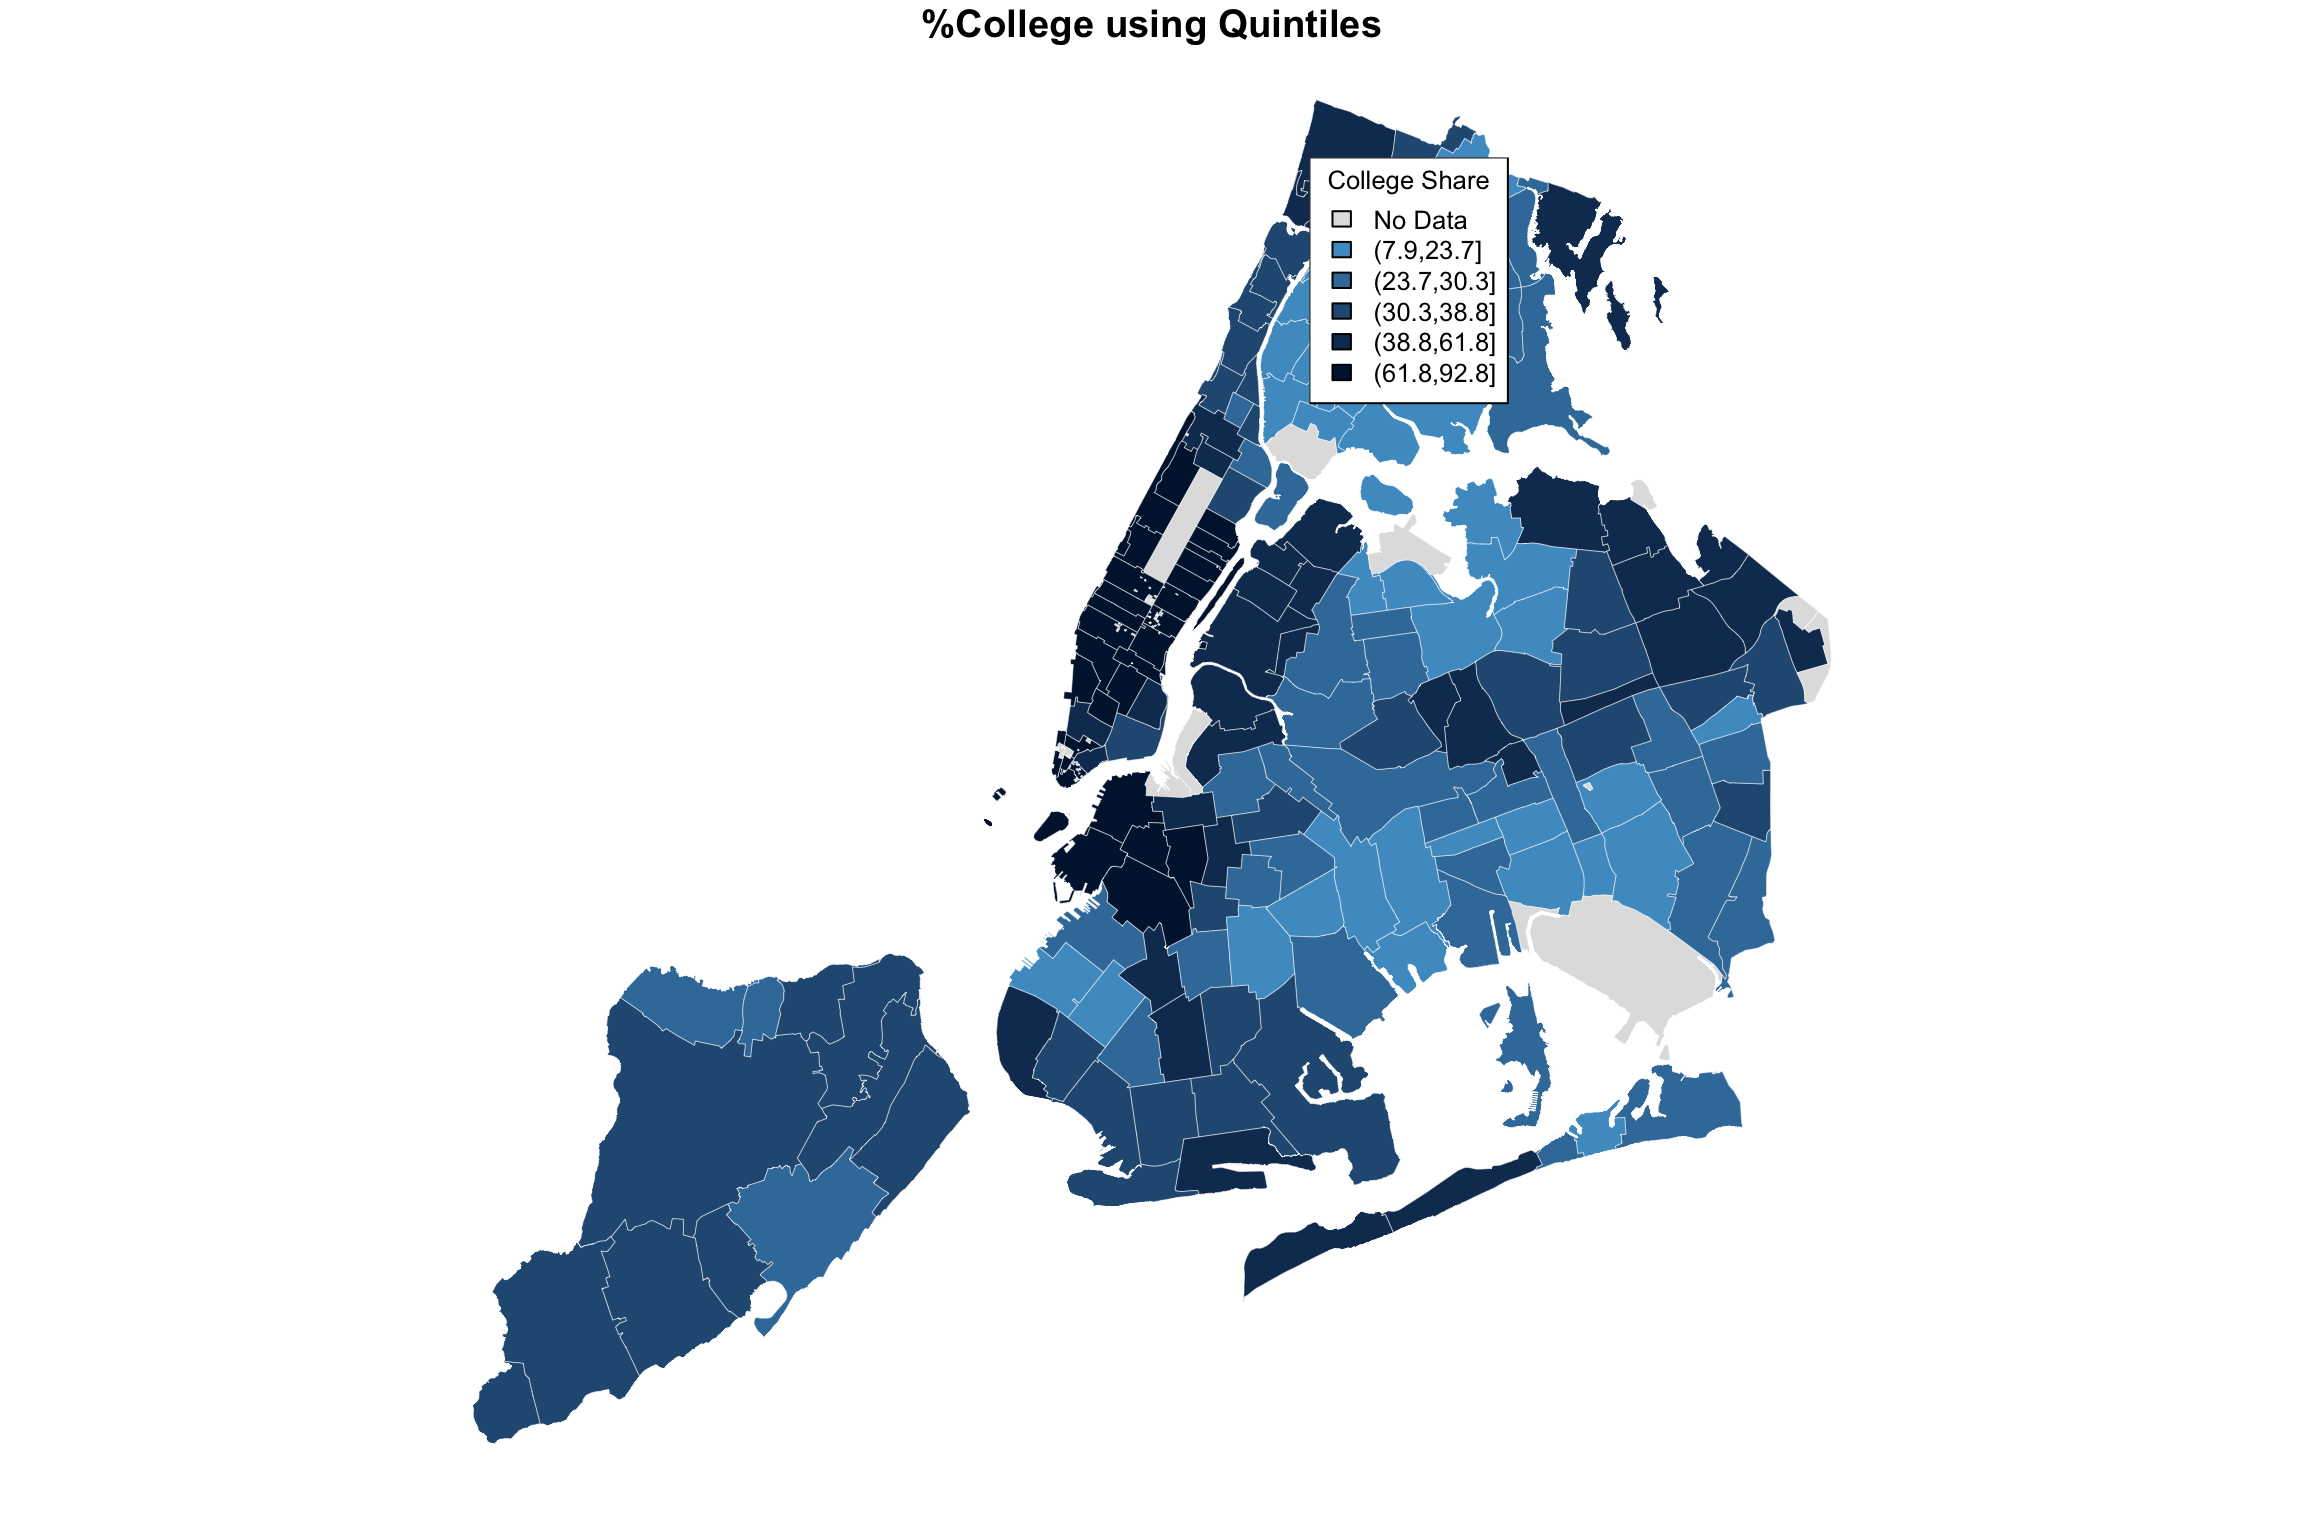
\includegraphics[width=0.9\linewidth]{carpedatum_files/figure-html/unnamed-chunk-93-1} \end{center}

\begin{Shaded}
\begin{Highlighting}[]
\FunctionTok{plot}\NormalTok{(NYC\_zips[,}\DecValTok{1}\NormalTok{], }\AttributeTok{col =}\NormalTok{ myShapeColors2}\SpecialCharTok{$}\NormalTok{regionValues, }
     \AttributeTok{main =} \StringTok{"\%College using Equal Intervals"}\NormalTok{, }
     \AttributeTok{cex =} \DecValTok{10}\NormalTok{, }\AttributeTok{border=}\StringTok{"white"}\NormalTok{, }\AttributeTok{lwd=}\FloatTok{0.25}\NormalTok{)}
\FunctionTok{legend}\NormalTok{(}\StringTok{"topleft"}\NormalTok{, }
       \AttributeTok{legend =}\NormalTok{ myShapeColors2}\SpecialCharTok{$}\NormalTok{legendText, }
       \AttributeTok{fill =}\NormalTok{ myShapeColors2}\SpecialCharTok{$}\NormalTok{legendColors, }\AttributeTok{cex =} \FloatTok{0.8}\NormalTok{, }\AttributeTok{title =} \StringTok{"College Share"}\NormalTok{)}
\end{Highlighting}
\end{Shaded}

\begin{center}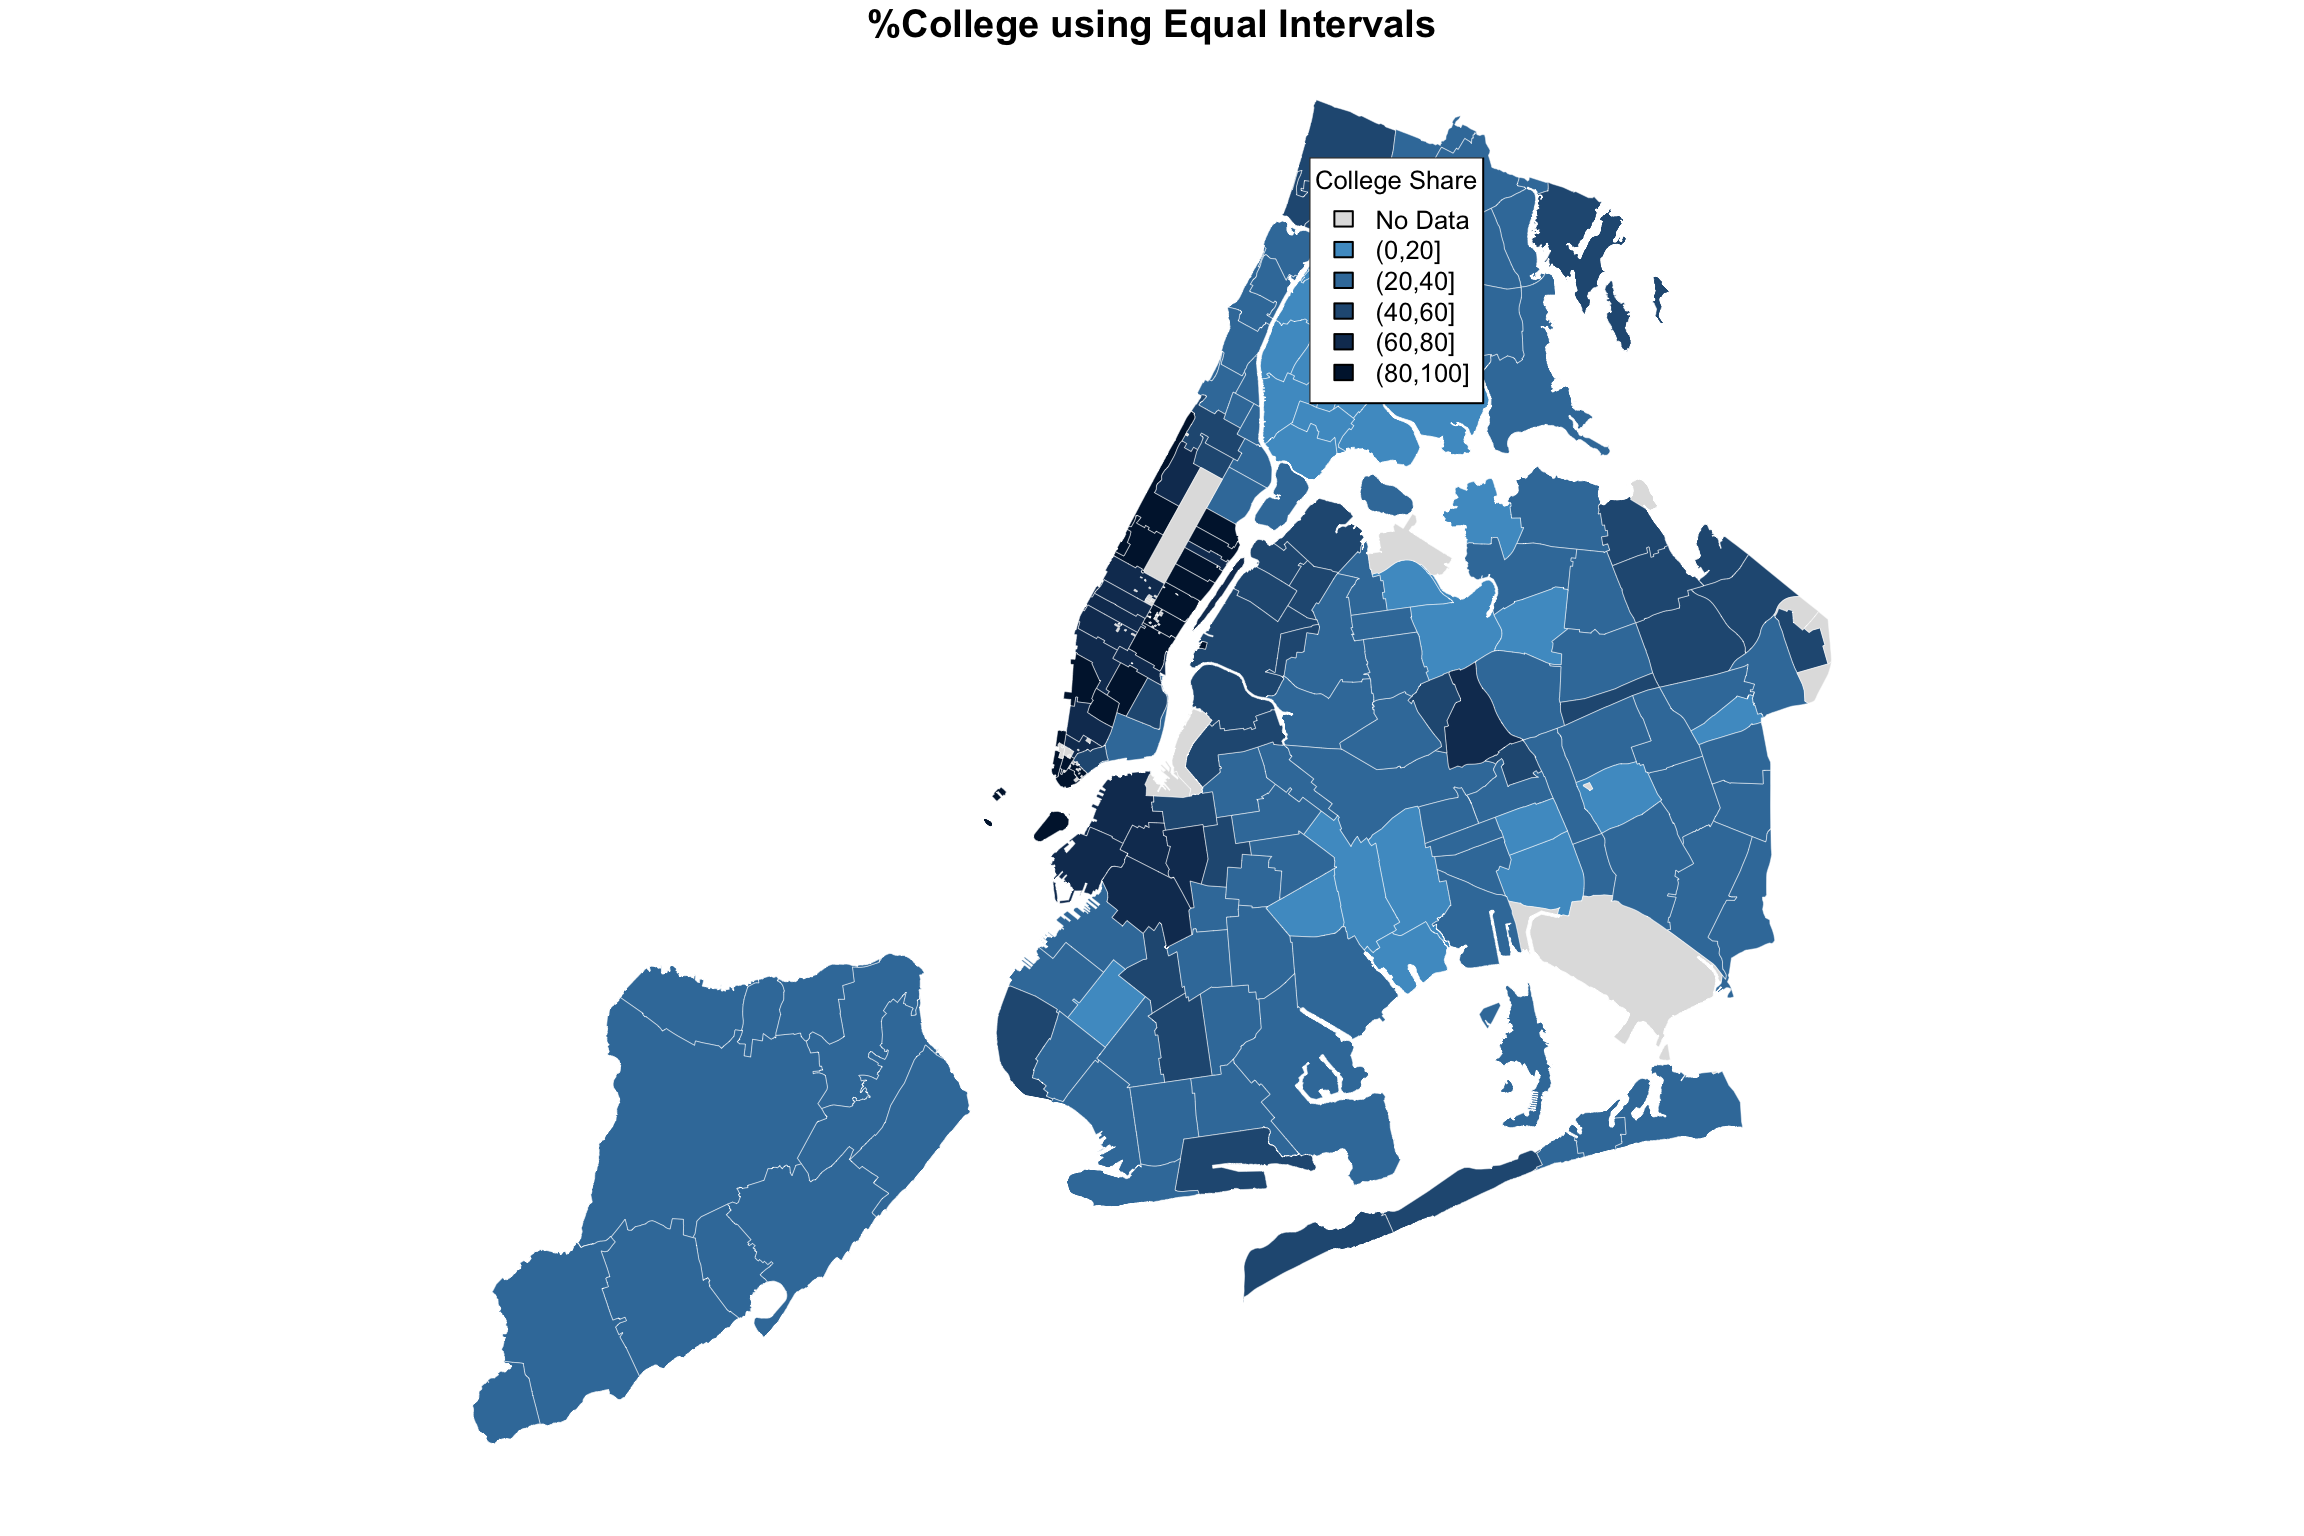
\includegraphics[width=0.9\linewidth]{carpedatum_files/figure-html/unnamed-chunk-93-2} \end{center}

The difference may be subtle, and I believe an argument can be made for either. But all in all, I believe that the level separation by quintiles does a better job in highlighting the difference between the different parts of the city.

This brings us to our next topic, which is comparing COVID-19 incidence maps to maps showing census data (e.g., income, college education, race, etc.)

\hypertarget{looking-at-two-variables-at-the-same-time}{%
\subsubsection*{Looking at two variables at the same time}\label{looking-at-two-variables-at-the-same-time}}
\addcontentsline{toc}{subsubsection}{Looking at two variables at the same time}

We can borrow the same side-by-side technique as above, but instead of the same data with different cut-points, we can plot two different variables. We'll use quintiles in both cases.

It turns out that population-adjusted COVID-19 rate is not actually in our data set. We need to make it, but it's easy.

\begin{Shaded}
\begin{Highlighting}[]
\NormalTok{covidPerCapita }\OtherTok{\textless{}{-}}\NormalTok{ mapData}\SpecialCharTok{$}\NormalTok{Positive}\SpecialCharTok{/}\NormalTok{mapData}\SpecialCharTok{$}\NormalTok{Total\_Pop}\SpecialCharTok{*}\DecValTok{100}
\FunctionTok{hist}\NormalTok{(covidPerCapita, }\AttributeTok{main=}\StringTok{"Zipcode{-}level Positive Cases Percent of Population"}\NormalTok{)}
\end{Highlighting}
\end{Shaded}

\begin{center}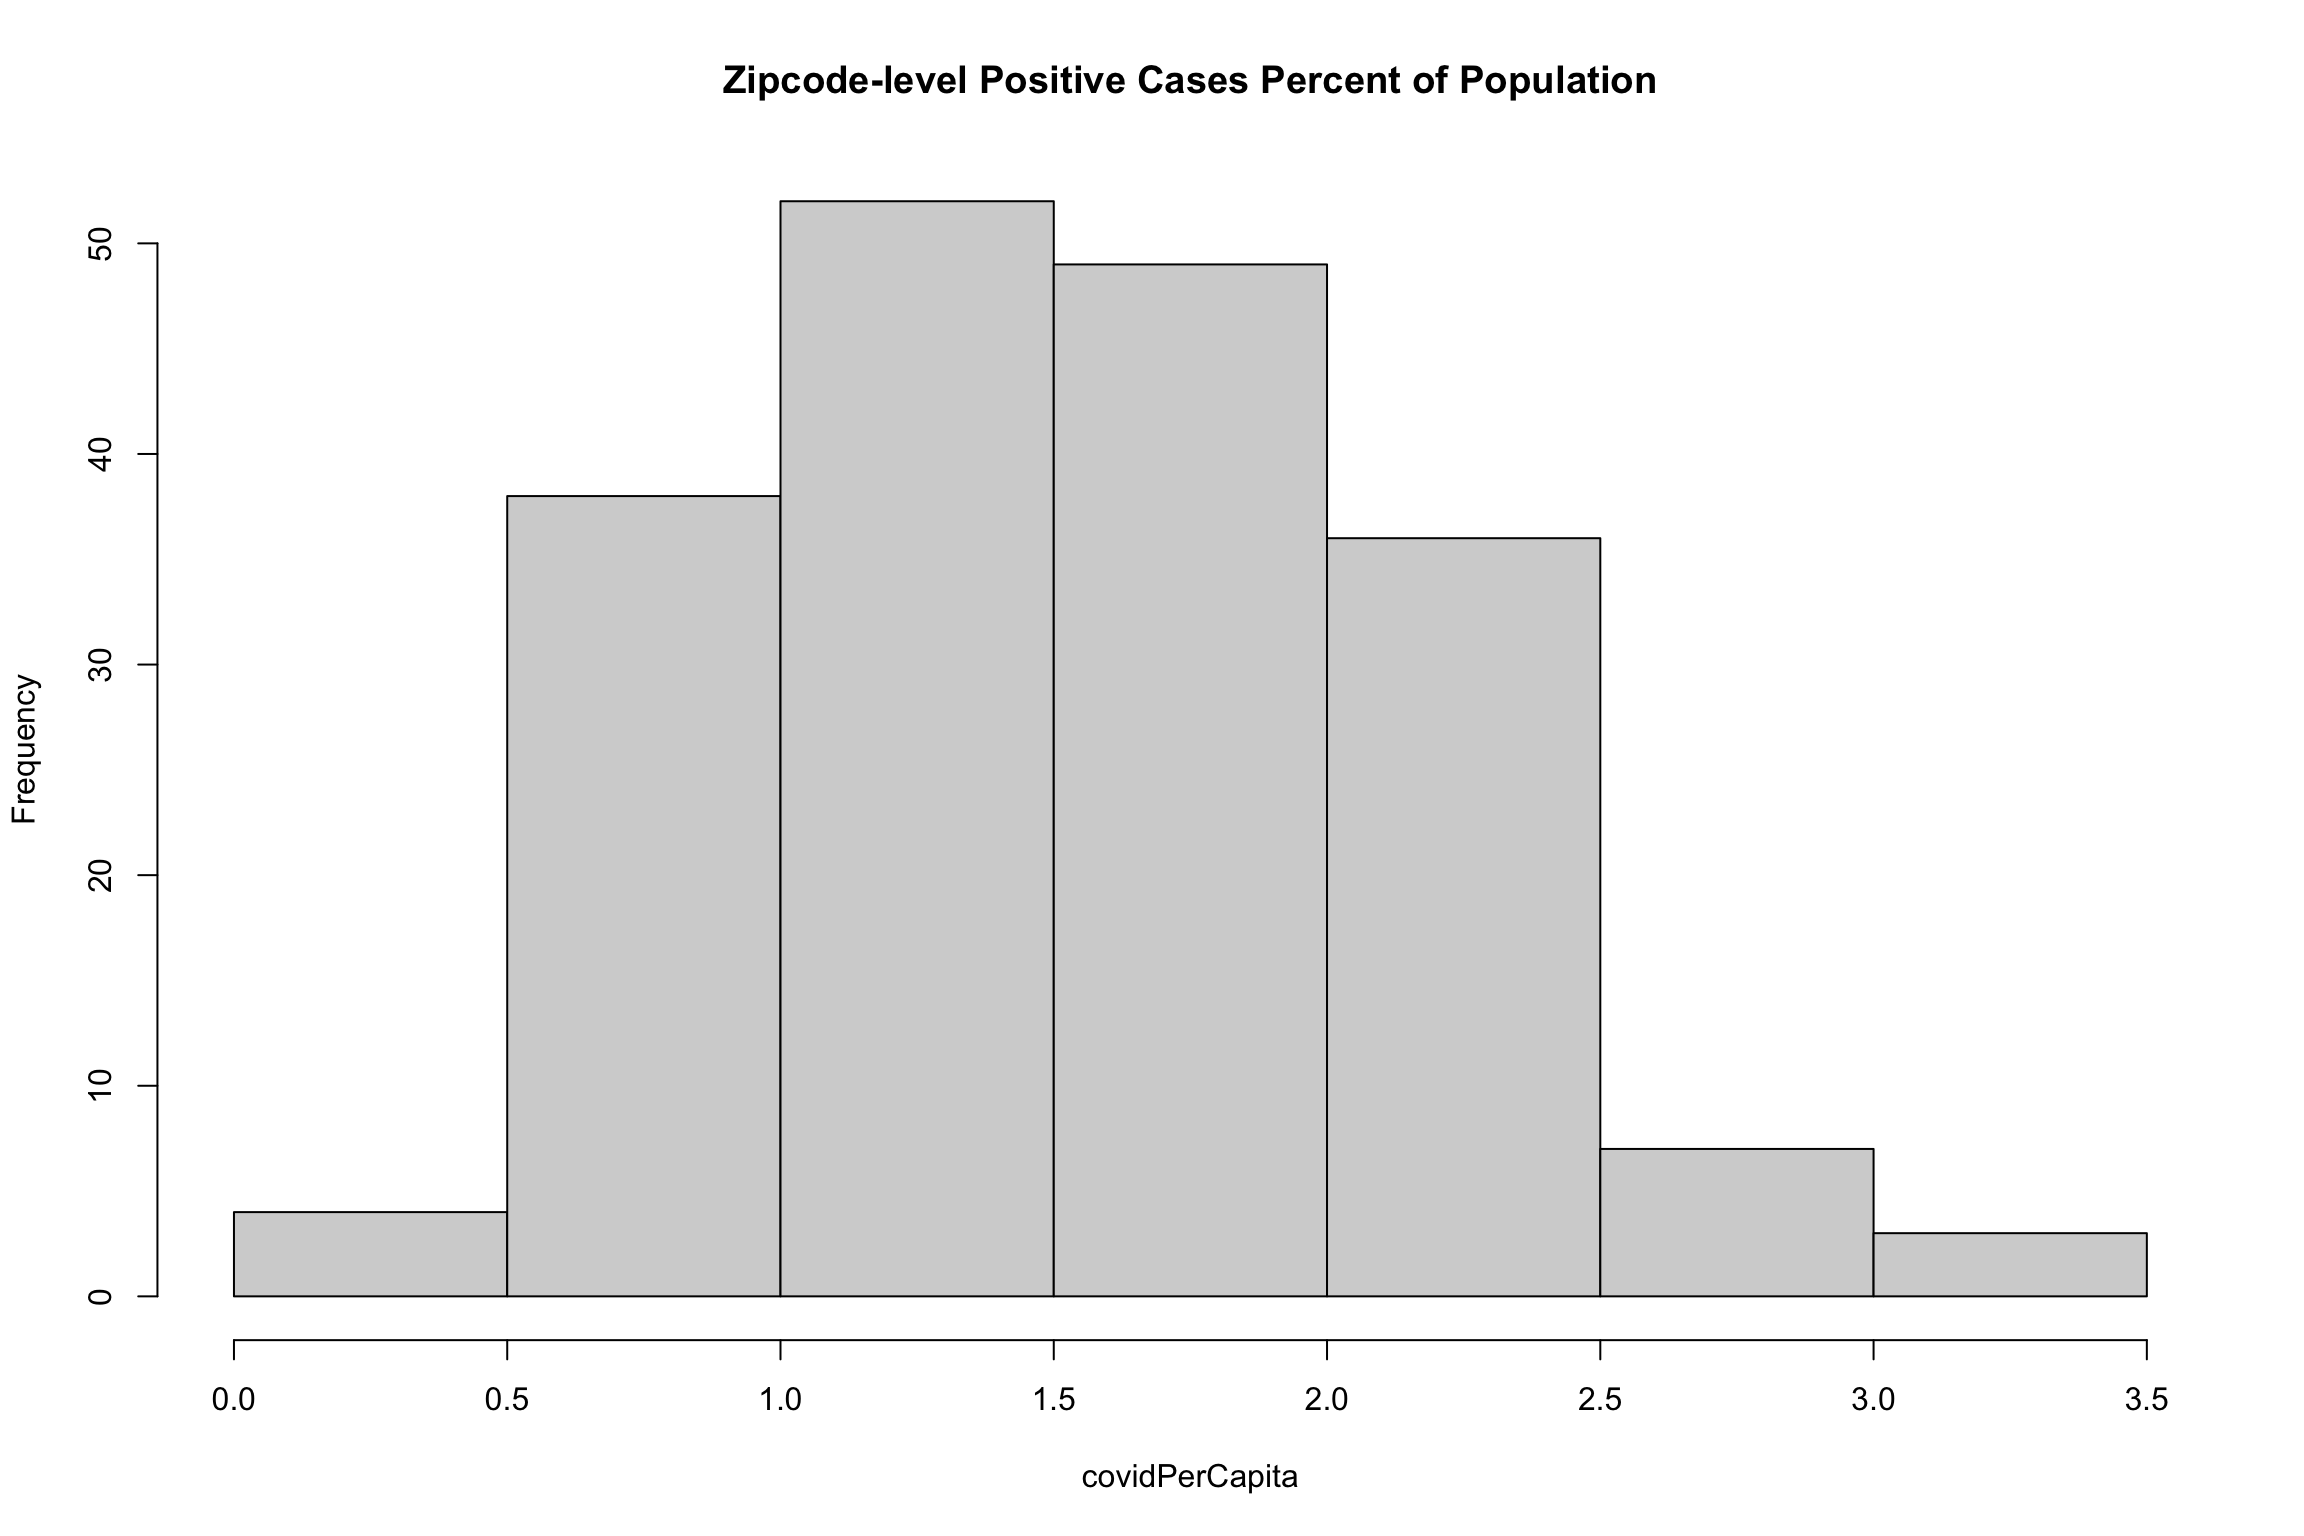
\includegraphics[width=0.9\linewidth]{carpedatum_files/figure-html/unnamed-chunk-94-1} \end{center}

\begin{Shaded}
\begin{Highlighting}[]
\NormalTok{myShapeColors1 }\OtherTok{\textless{}{-}} \FunctionTok{getShapeColors}\NormalTok{(covidPerCapita, }\AttributeTok{nbreaks=}\DecValTok{5}\NormalTok{)}
\NormalTok{myShapeColors2 }\OtherTok{\textless{}{-}} \FunctionTok{getShapeColors}\NormalTok{(bachelorPlus, }\AttributeTok{nbreaks=}\DecValTok{5}\NormalTok{)}

\FunctionTok{par}\NormalTok{(}\AttributeTok{mfrow=}\FunctionTok{c}\NormalTok{(}\DecValTok{1}\NormalTok{,}\DecValTok{2}\NormalTok{))}

\FunctionTok{plot}\NormalTok{(NYC\_zips[,}\DecValTok{1}\NormalTok{], }\AttributeTok{col =}\NormalTok{ myShapeColors1}\SpecialCharTok{$}\NormalTok{regionValues, }
     \AttributeTok{main =} \StringTok{"\%COVID Cases"}\NormalTok{, }
     \AttributeTok{cex =} \DecValTok{10}\NormalTok{, }\AttributeTok{border=}\StringTok{"white"}\NormalTok{, }\AttributeTok{lwd=}\FloatTok{0.25}\NormalTok{)}
\FunctionTok{legend}\NormalTok{(}\StringTok{"topleft"}\NormalTok{, }
       \AttributeTok{legend =}\NormalTok{ myShapeColors1}\SpecialCharTok{$}\NormalTok{legendText, }
       \AttributeTok{fill =}\NormalTok{ myShapeColors1}\SpecialCharTok{$}\NormalTok{legendColors, }\AttributeTok{cex =} \FloatTok{0.8}\NormalTok{, }\AttributeTok{title =} \StringTok{"COVID rate"}\NormalTok{)}
\end{Highlighting}
\end{Shaded}

\begin{center}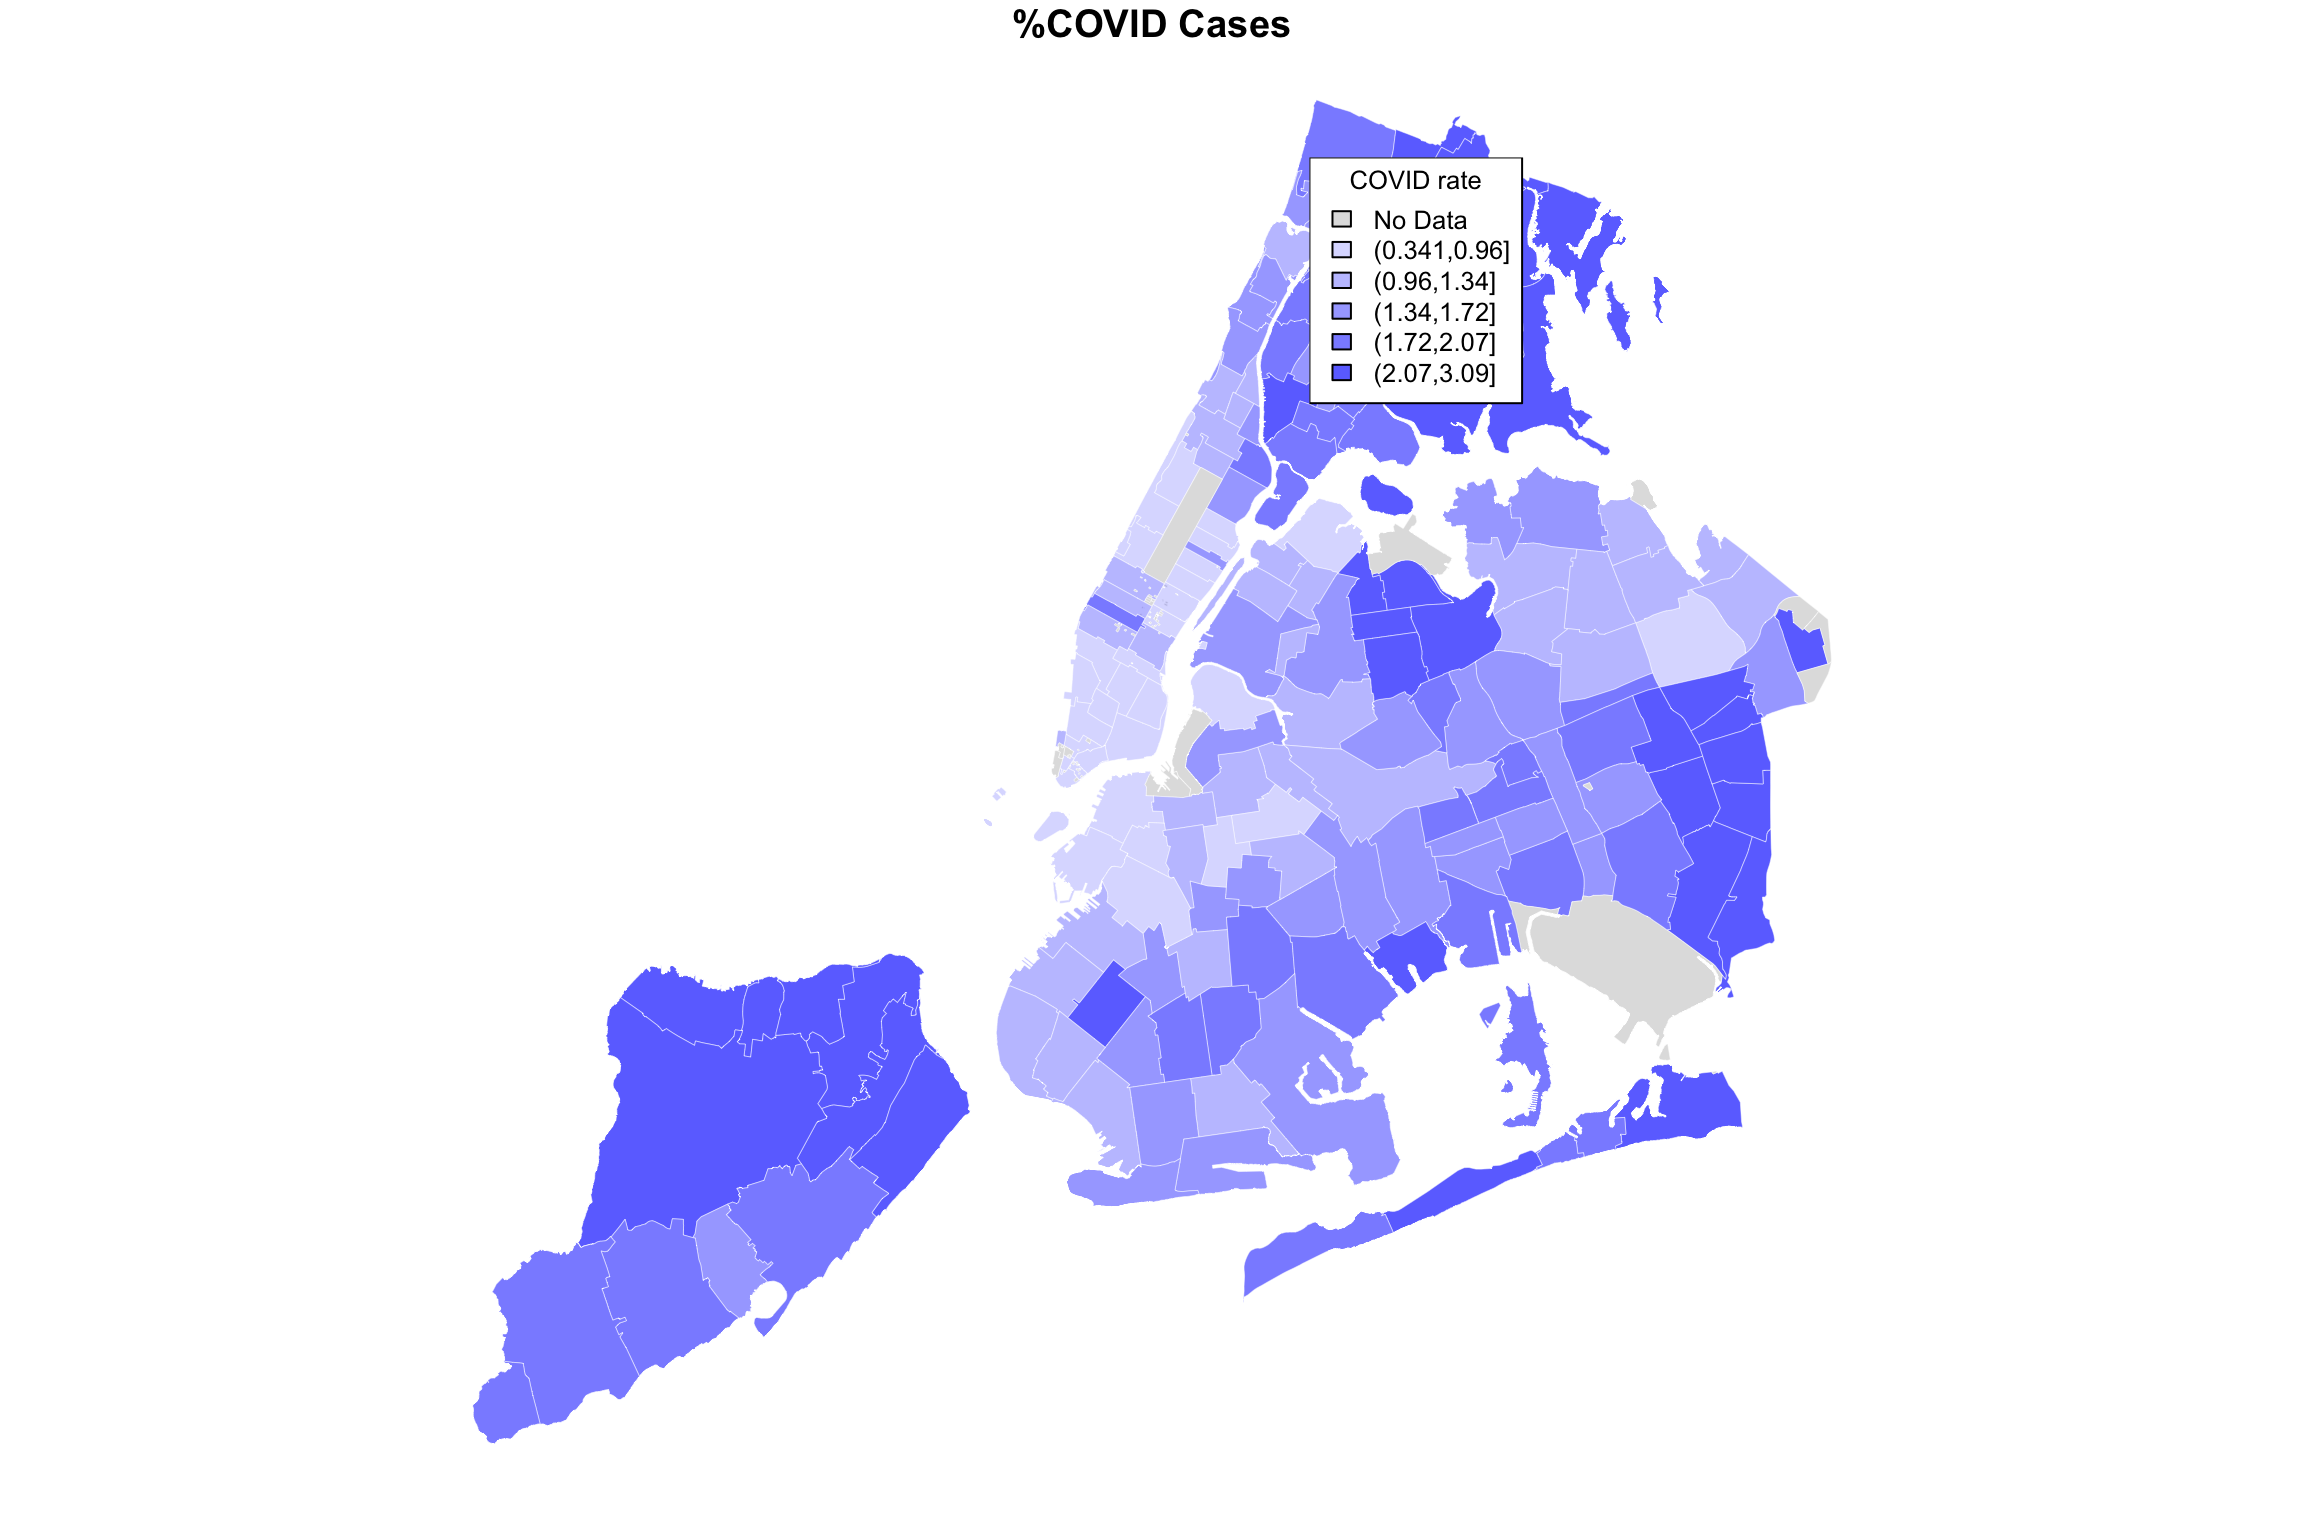
\includegraphics[width=0.9\linewidth]{carpedatum_files/figure-html/unnamed-chunk-95-1} \end{center}

\begin{Shaded}
\begin{Highlighting}[]
\FunctionTok{plot}\NormalTok{(NYC\_zips[,}\DecValTok{1}\NormalTok{], }\AttributeTok{col =}\NormalTok{ myShapeColors2}\SpecialCharTok{$}\NormalTok{regionValues, }
     \AttributeTok{main =} \StringTok{"\%College"}\NormalTok{, }
     \AttributeTok{cex =} \DecValTok{10}\NormalTok{, }\AttributeTok{border=}\StringTok{"white"}\NormalTok{, }\AttributeTok{lwd=}\FloatTok{0.25}\NormalTok{)}
\FunctionTok{legend}\NormalTok{(}\StringTok{"topleft"}\NormalTok{, }
       \AttributeTok{legend =}\NormalTok{ myShapeColors2}\SpecialCharTok{$}\NormalTok{legendText, }
       \AttributeTok{fill =}\NormalTok{ myShapeColors2}\SpecialCharTok{$}\NormalTok{legendColors, }\AttributeTok{cex =} \FloatTok{0.8}\NormalTok{, }\AttributeTok{title =} \StringTok{"College Share"}\NormalTok{)}
\end{Highlighting}
\end{Shaded}

\begin{center}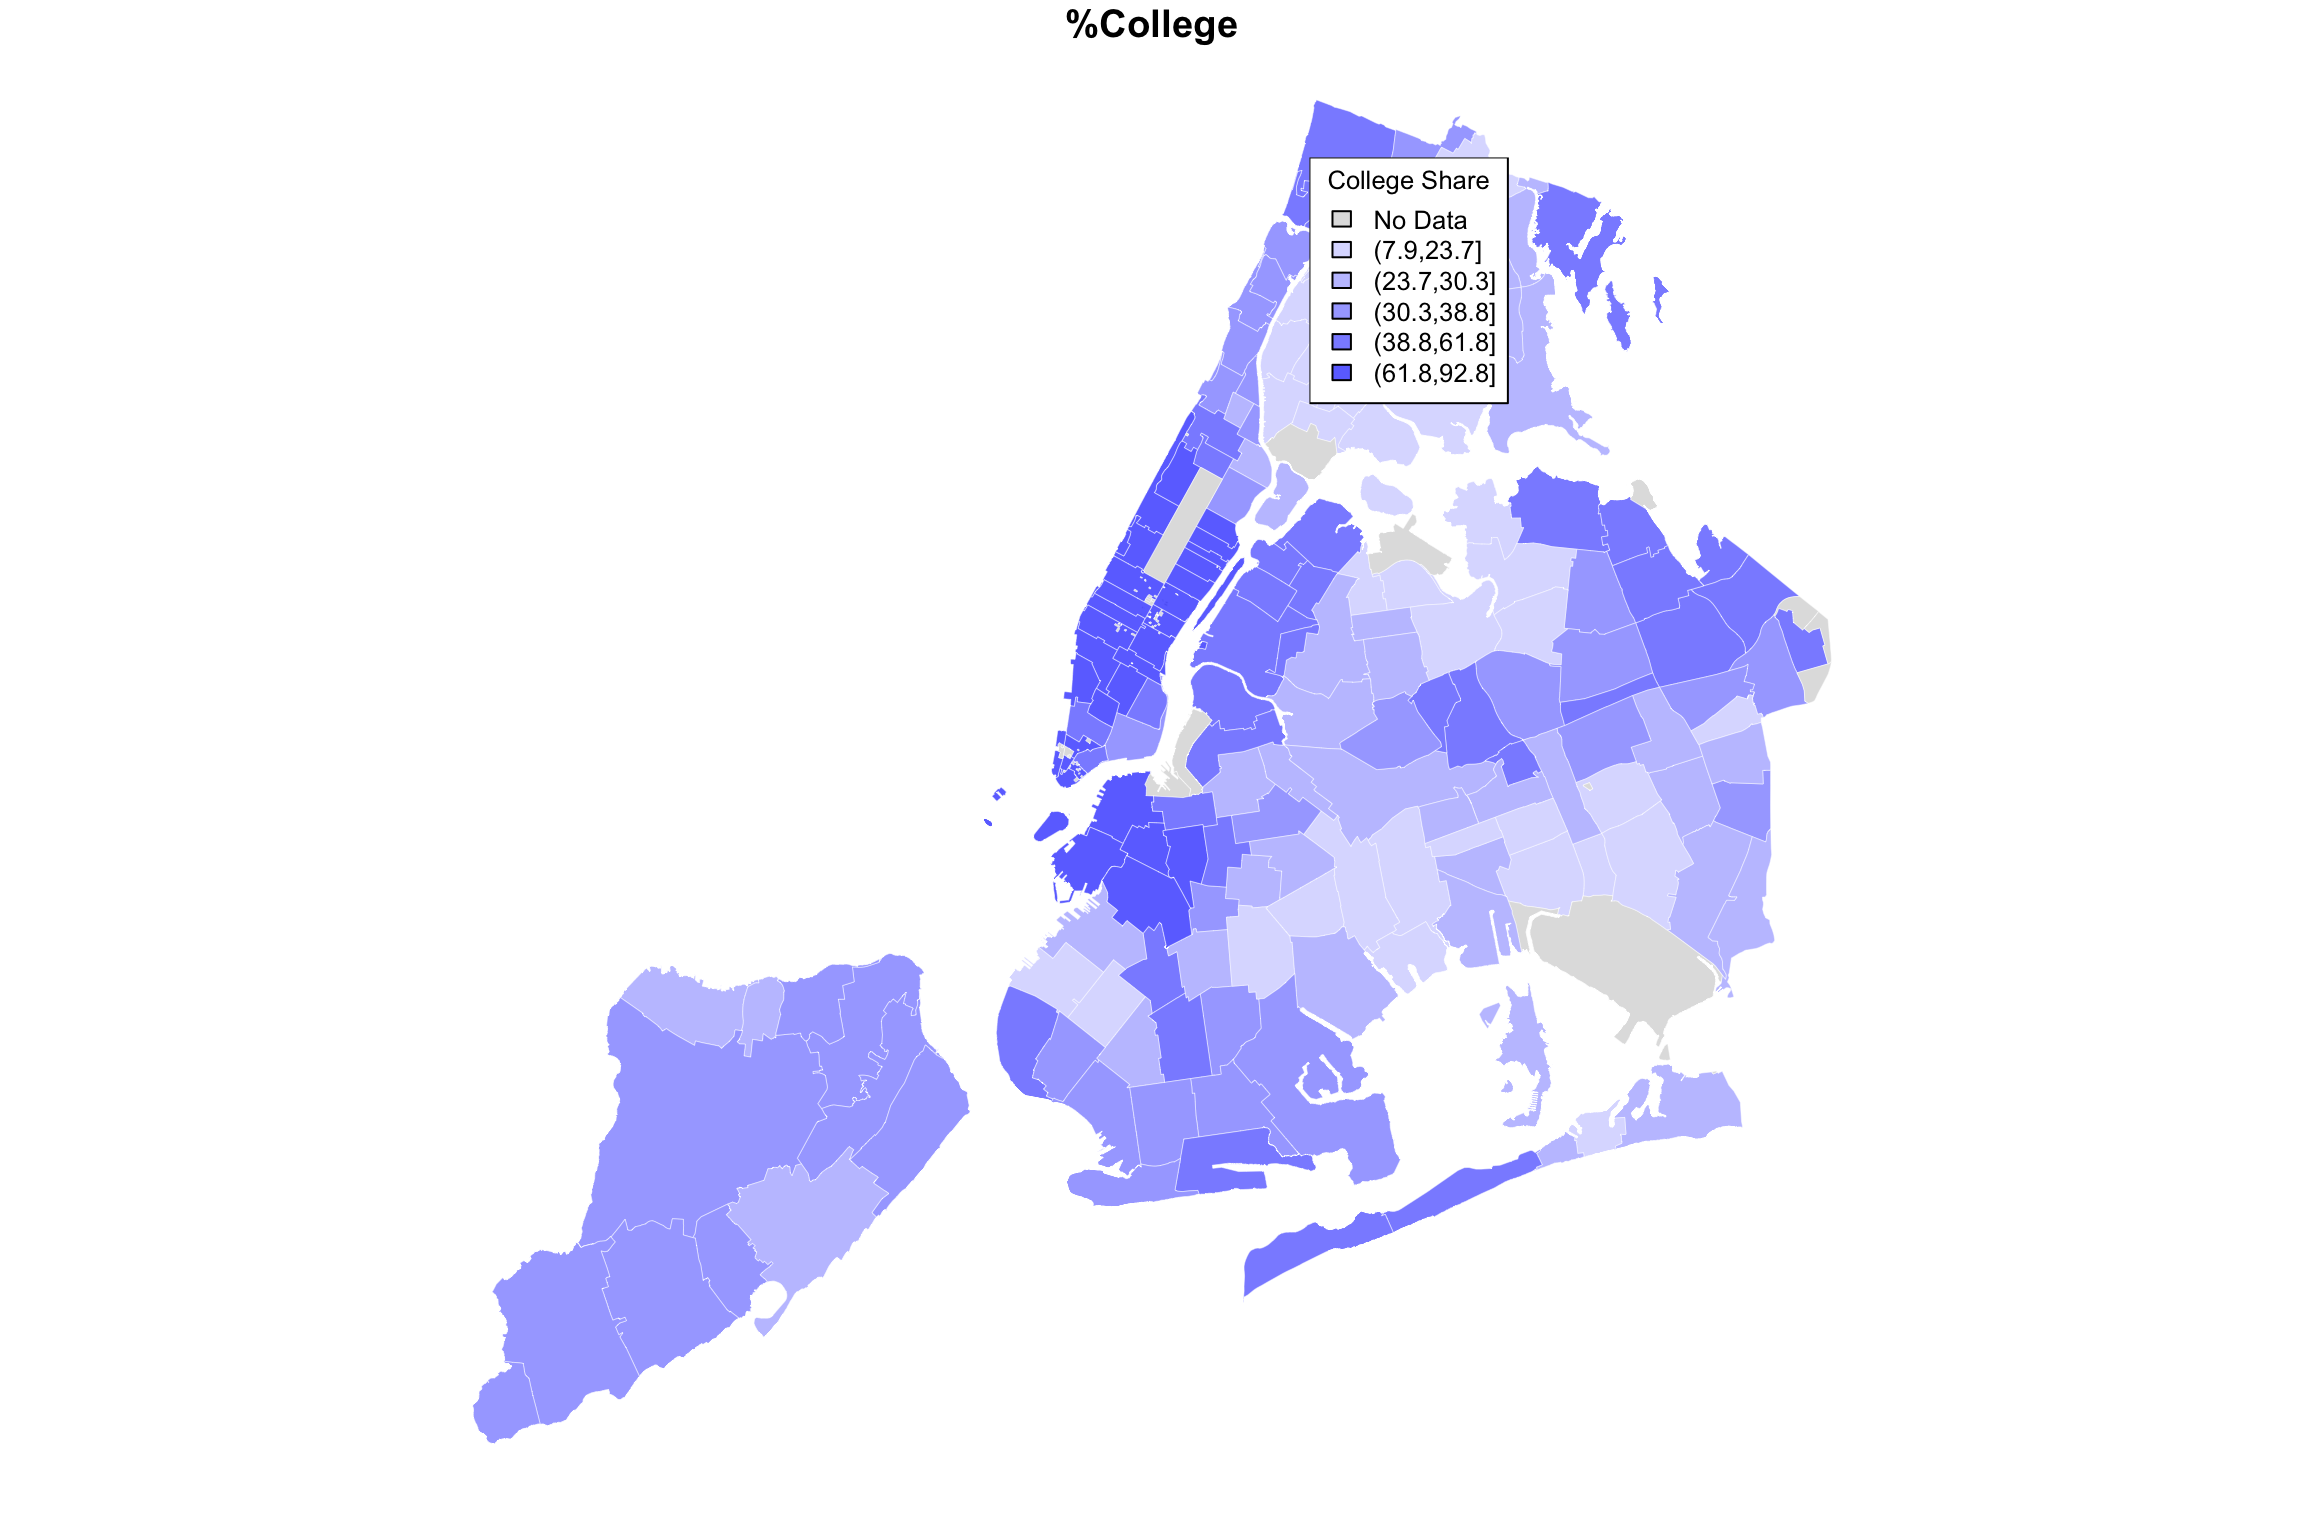
\includegraphics[width=0.9\linewidth]{carpedatum_files/figure-html/unnamed-chunk-95-2} \end{center}

Now we're looking at two different variables, both mapped using quintiles as an organizer of zipcode-level data. It definitely seems like one map is almost an inverse of the other. Where COVID rate is high, college rate is low, and vice versa. Is there some way for us to see both variables on the same map at the same time?

Here's one idea. Suppose we used different colors for each variable, e.g.~red and blue, but we used shades from lighter to darker to indicate lowr and higher values. And suppose we made the colors transparent, the way we did when we plotted two histograms on the same plot. When pink and light-blue are both laid over each other, we will see a purplish color. Therefore

\begin{enumerate}
\def\labelenumi{\arabic{enumi}.}
\tightlist
\item
  If both variables are high, we will have darker purple
\item
  If both variables are low, we will have lighter purple
\item
  If one variable is high and the other low, we will see regions of red or blue
\end{enumerate}

So what happens if we ``add'' up the two variable maps this way?

\begin{Shaded}
\begin{Highlighting}[]
\NormalTok{myShapeColorsCovid }\OtherTok{\textless{}{-}} \FunctionTok{getShapeColors}\NormalTok{(covidPerCapita, }\AttributeTok{nbreaks=}\DecValTok{5}\NormalTok{, }\AttributeTok{rdgrbl=}\FunctionTok{c}\NormalTok{(}\DecValTok{1}\NormalTok{,}\DecValTok{0}\NormalTok{,}\DecValTok{0}\NormalTok{))}
\NormalTok{myShapeColorsCollege }\OtherTok{\textless{}{-}} \FunctionTok{getShapeColors}\NormalTok{(bachelorPlus, }\AttributeTok{nbreaks=}\DecValTok{5}\NormalTok{, }\AttributeTok{rdgrbl=}\FunctionTok{c}\NormalTok{(}\DecValTok{0}\NormalTok{,}\DecValTok{0}\NormalTok{,}\DecValTok{1}\NormalTok{))}

\FunctionTok{par}\NormalTok{(}\AttributeTok{mfrow=}\FunctionTok{c}\NormalTok{(}\DecValTok{1}\NormalTok{,}\DecValTok{3}\NormalTok{))}
\FunctionTok{plot}\NormalTok{(NYC\_zips[,}\DecValTok{1}\NormalTok{], }\AttributeTok{col =}\NormalTok{ myShapeColorsCovid}\SpecialCharTok{$}\NormalTok{regionValues, }\AttributeTok{main =} \StringTok{"covid"}\NormalTok{, }
     \AttributeTok{cex =} \DecValTok{10}\NormalTok{, }\AttributeTok{lwd=}\FloatTok{0.05}\NormalTok{)}
\end{Highlighting}
\end{Shaded}

\begin{center}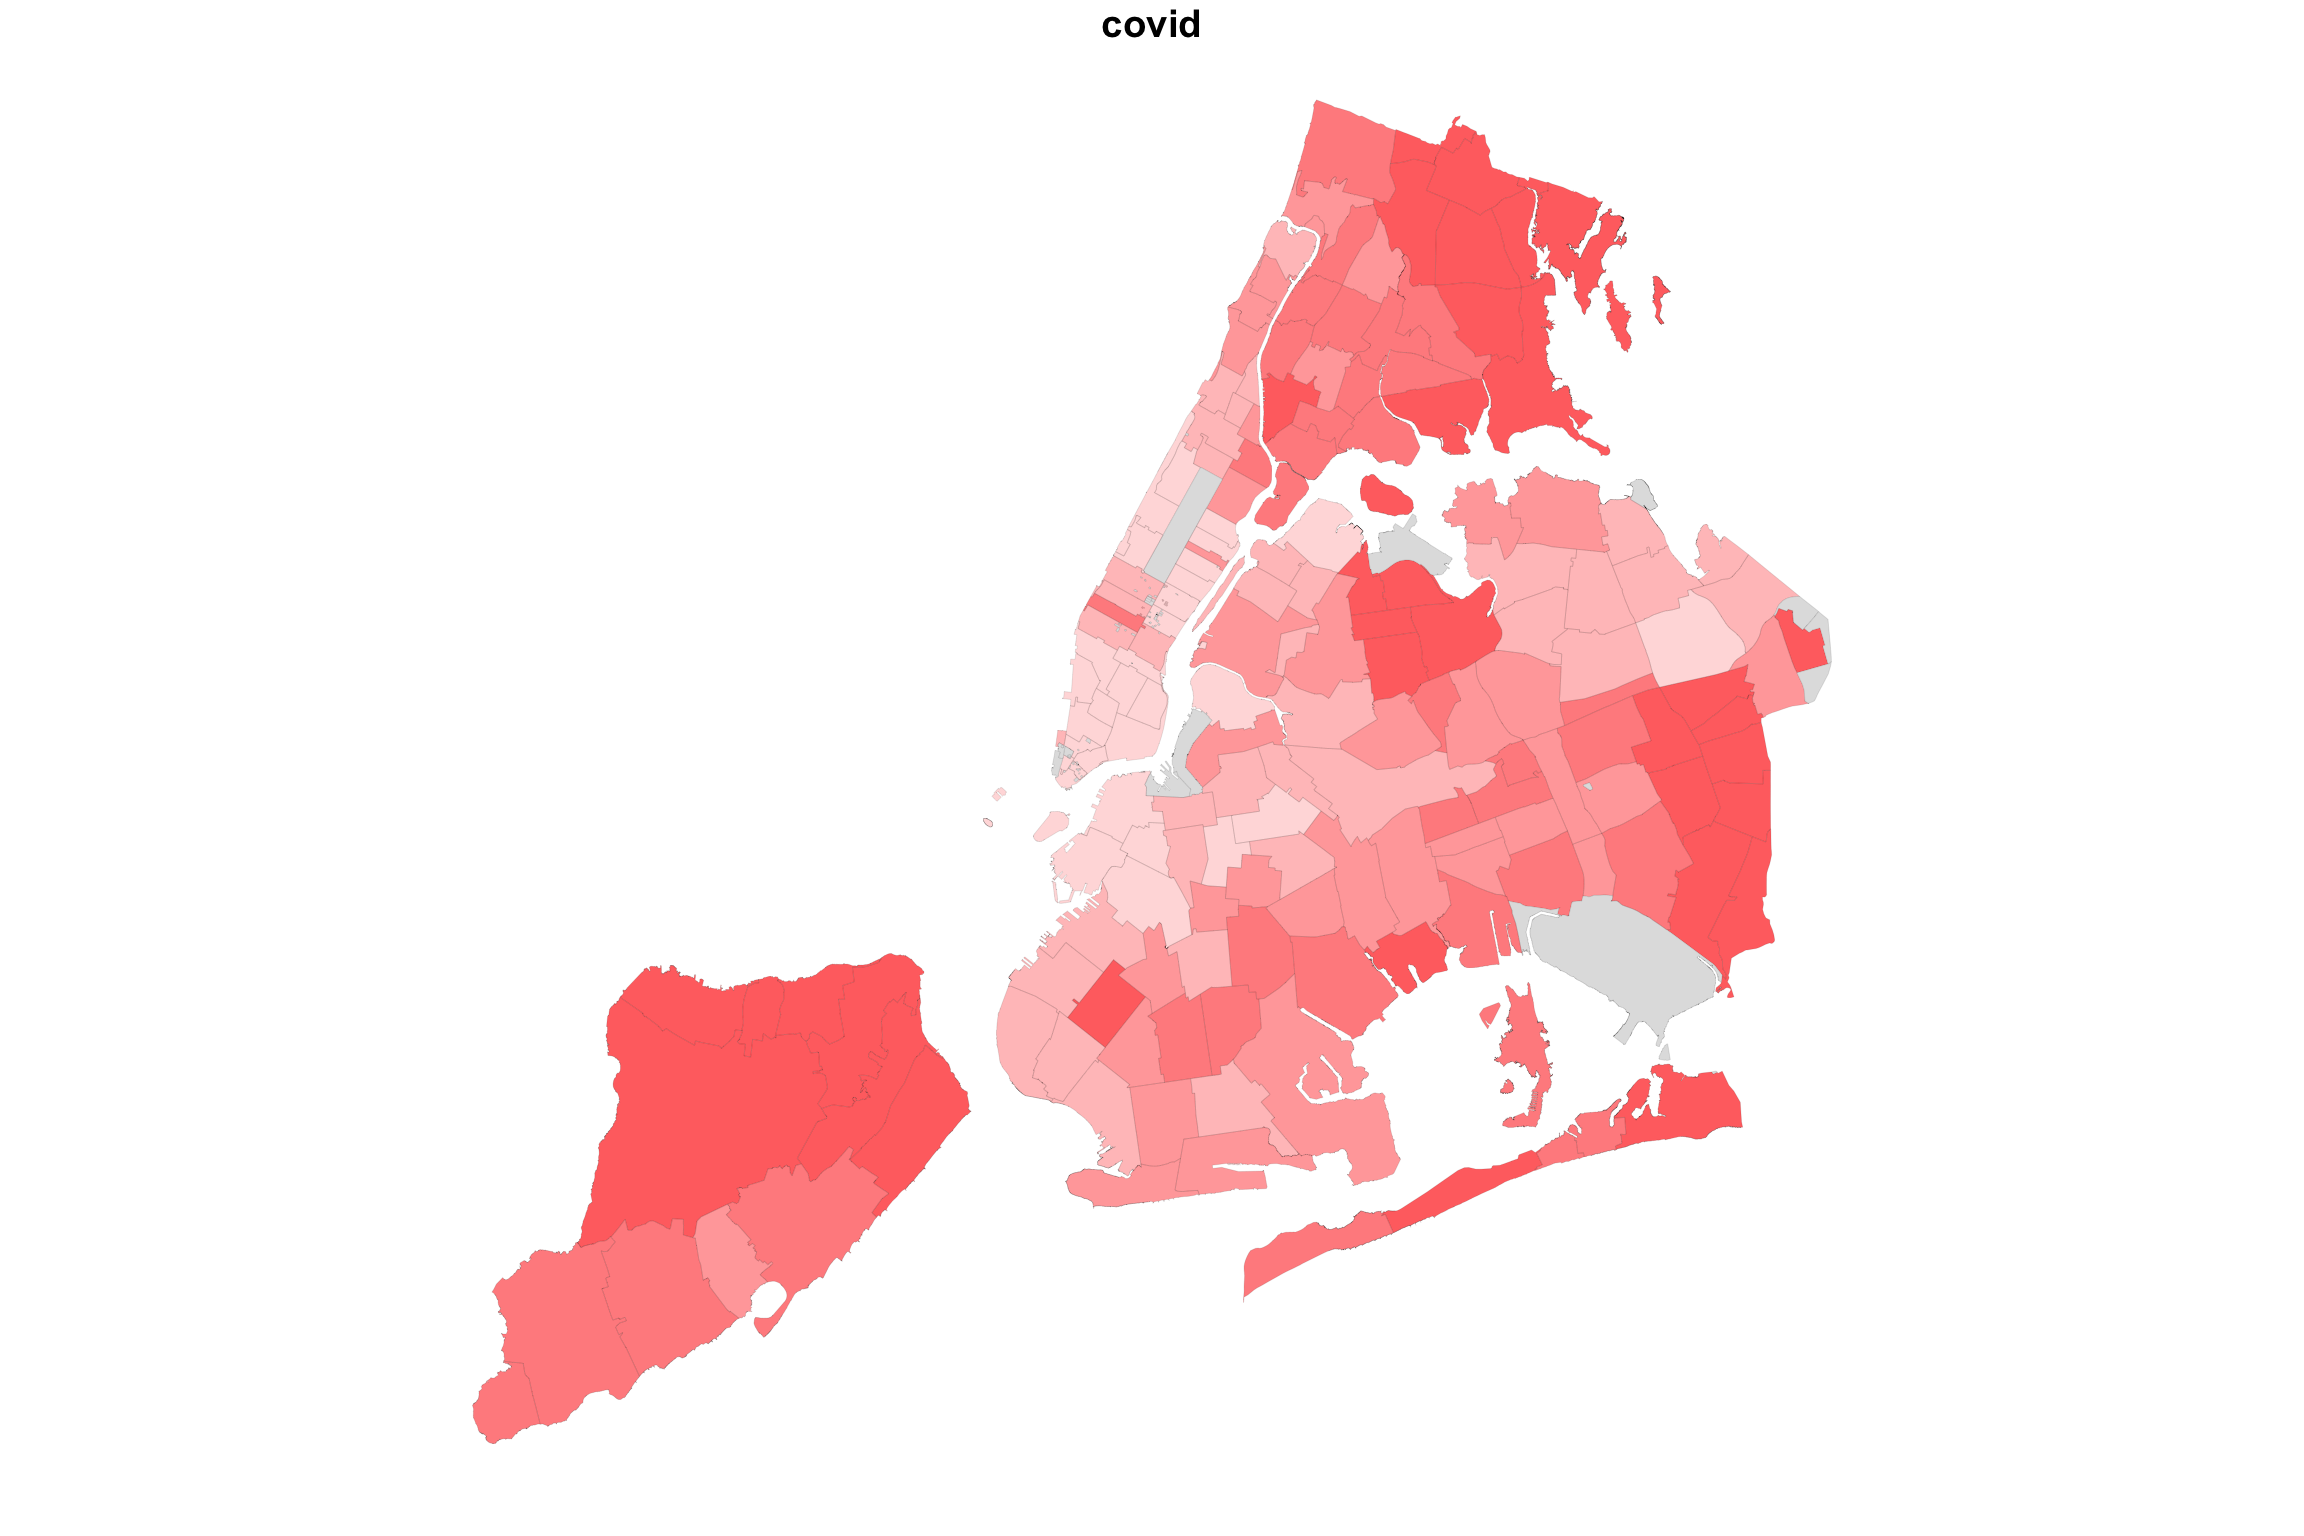
\includegraphics[width=0.9\linewidth]{carpedatum_files/figure-html/unnamed-chunk-96-1} \end{center}

\begin{Shaded}
\begin{Highlighting}[]
\FunctionTok{plot}\NormalTok{(NYC\_zips[,}\DecValTok{1}\NormalTok{], }\AttributeTok{col =}\NormalTok{ myShapeColorsCollege}\SpecialCharTok{$}\NormalTok{regionValues, }\AttributeTok{main =} \StringTok{"college"}\NormalTok{, }
     \AttributeTok{cex =} \DecValTok{10}\NormalTok{, }\AttributeTok{lwd=}\FloatTok{0.05}\NormalTok{) }
\end{Highlighting}
\end{Shaded}

\begin{center}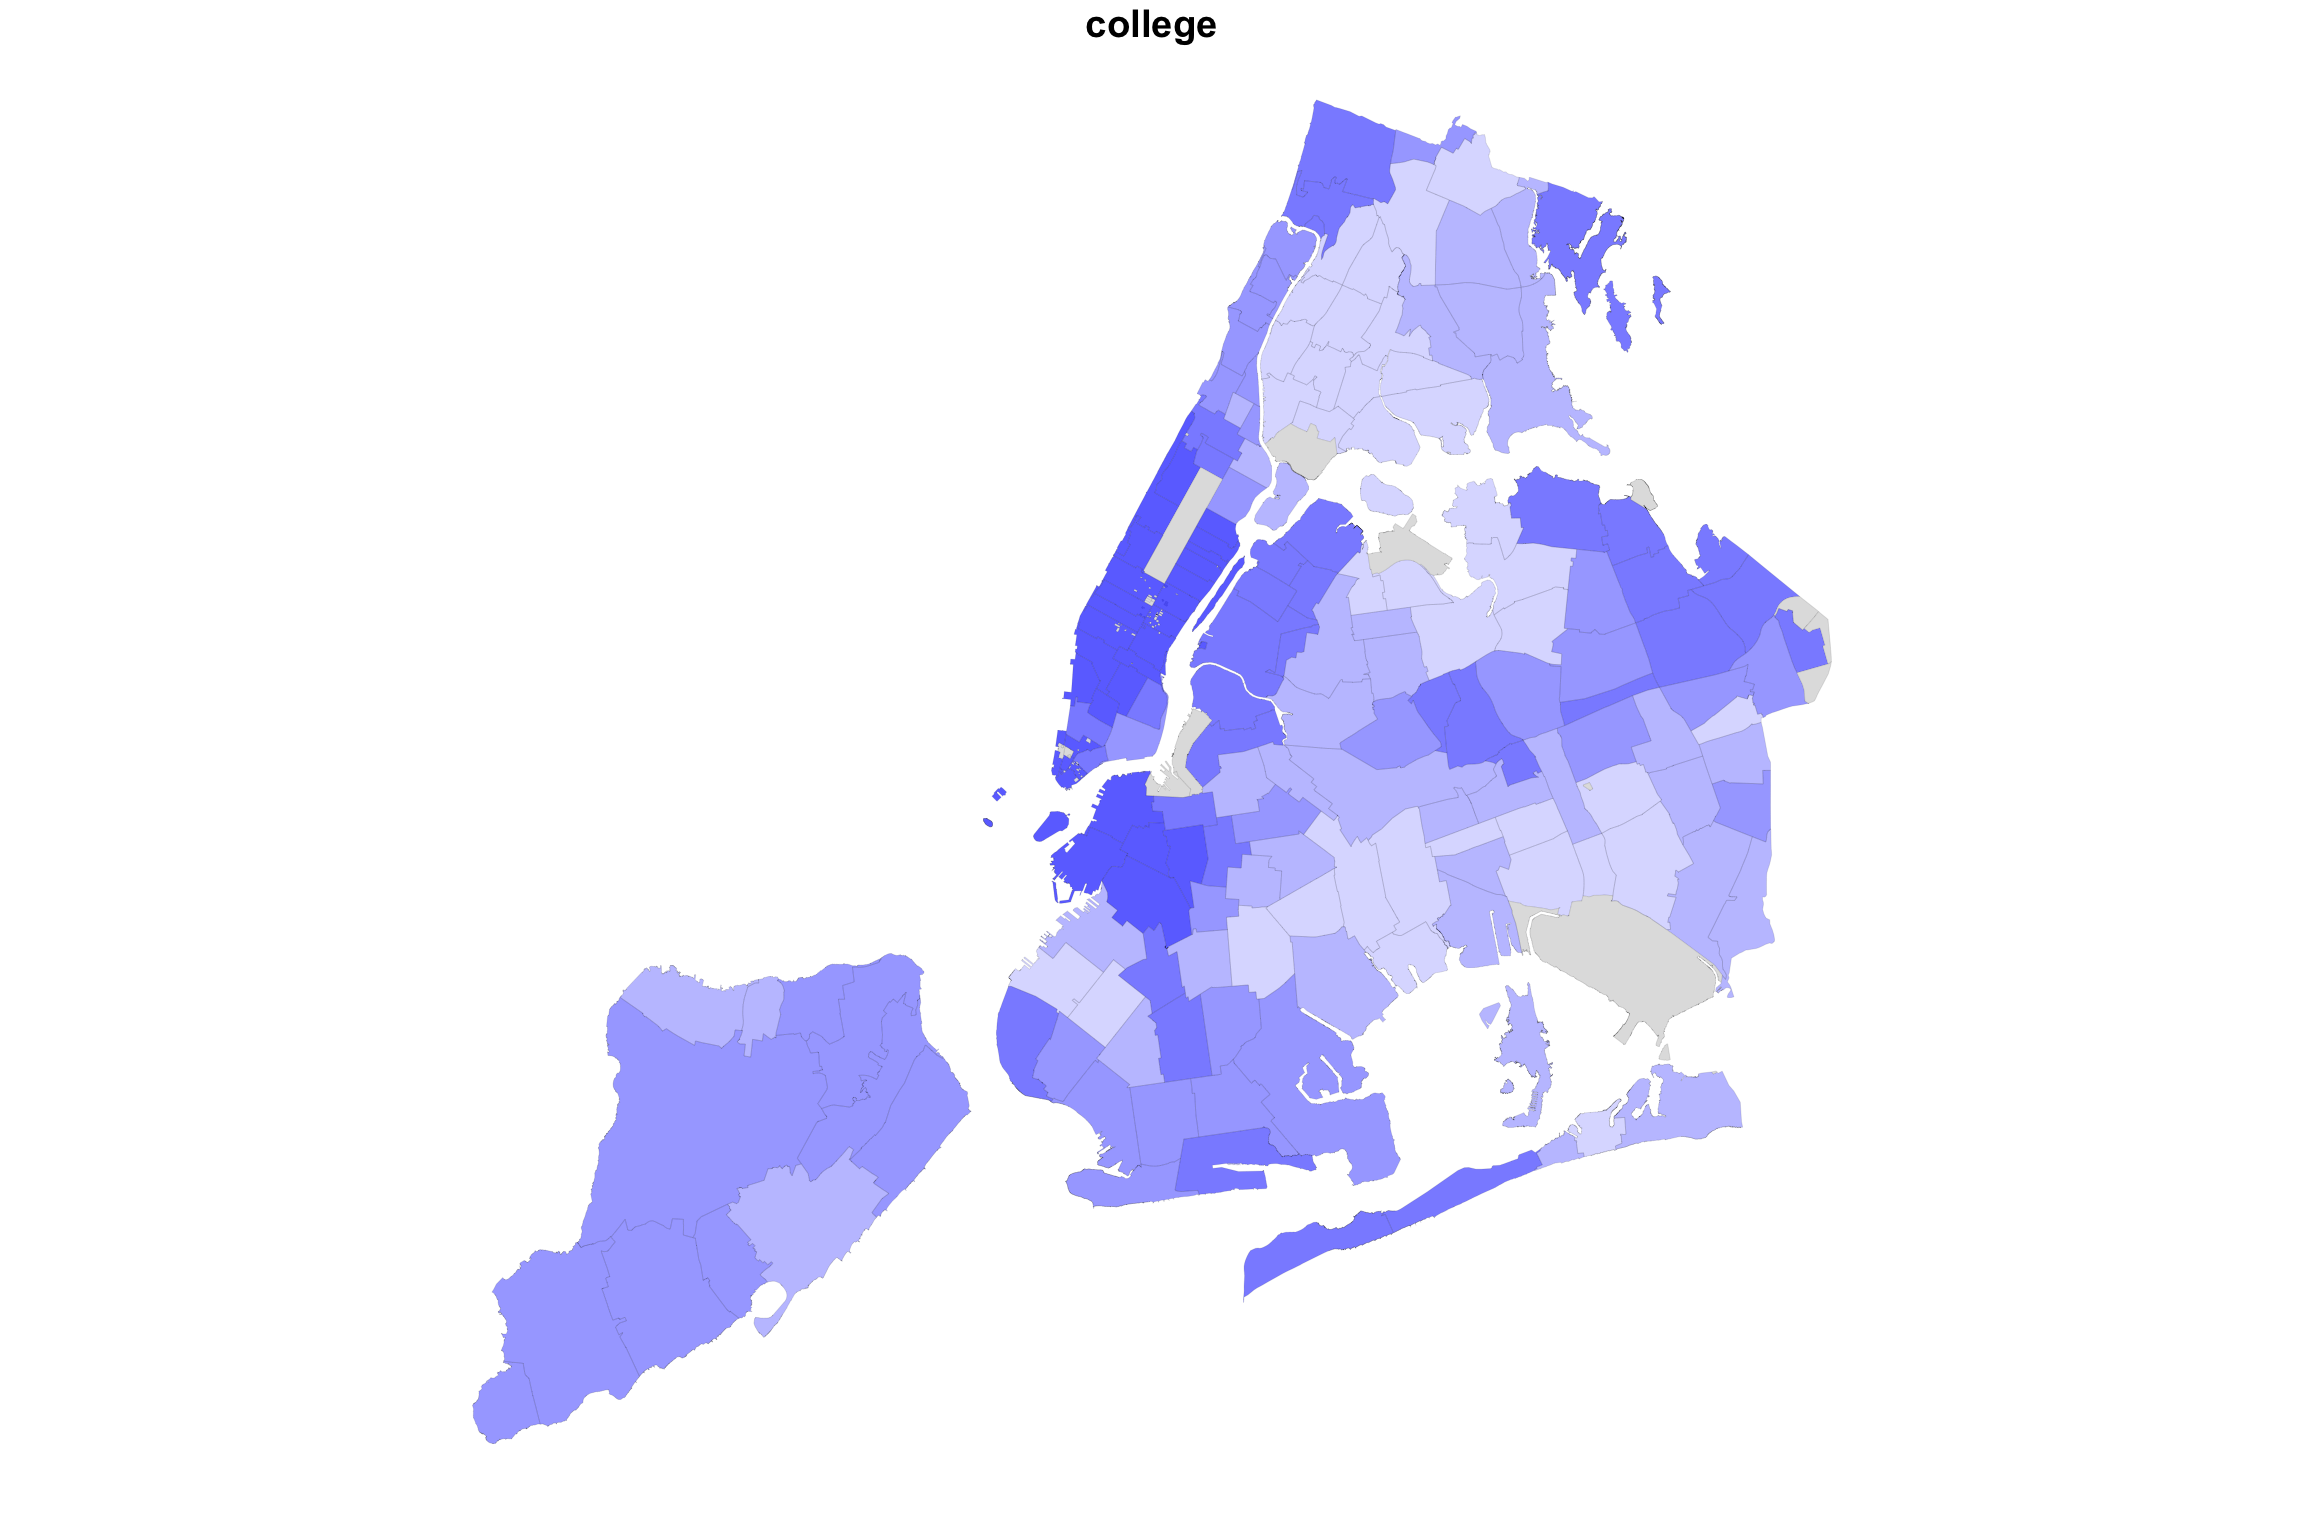
\includegraphics[width=0.9\linewidth]{carpedatum_files/figure-html/unnamed-chunk-96-2} \end{center}

\begin{Shaded}
\begin{Highlighting}[]
\FunctionTok{plot}\NormalTok{(NYC\_zips[,}\DecValTok{1}\NormalTok{], }\AttributeTok{col =}\NormalTok{ myShapeColorsCovid}\SpecialCharTok{$}\NormalTok{regionValues, }\AttributeTok{main =} \StringTok{"covid+college"}\NormalTok{, }
     \AttributeTok{cex =} \DecValTok{10}\NormalTok{, }\AttributeTok{lwd=}\FloatTok{0.05}\NormalTok{)}
\FunctionTok{plot}\NormalTok{(NYC\_zips[,}\DecValTok{1}\NormalTok{], }\AttributeTok{col =}\NormalTok{ myShapeColorsCollege}\SpecialCharTok{$}\NormalTok{regionValues, }\AttributeTok{add=}\NormalTok{T, }
     \AttributeTok{cex =} \DecValTok{10}\NormalTok{, }\AttributeTok{lwd=}\FloatTok{0.05}\NormalTok{)}
\end{Highlighting}
\end{Shaded}

\begin{center}\includegraphics[width=0.9\linewidth]{carpedatum_files/figure-html/unnamed-chunk-96-3} \end{center}

In the case of college education and COVID incidence rates, the variables are negatively associated. Overlaying two color maps, we see red and bluish regions, but we also see some purple stuff.

What would happen if we did the same for two variable with positive association? Let us map COVID-19 incidence against the average household size.

\begin{Shaded}
\begin{Highlighting}[]
\NormalTok{myShapeColorsCovid }\OtherTok{\textless{}{-}} \FunctionTok{getShapeColors}\NormalTok{(covidPerCapita, }\AttributeTok{nbreaks=}\DecValTok{5}\NormalTok{, }\AttributeTok{rdgrbl=}\FunctionTok{c}\NormalTok{(}\DecValTok{1}\NormalTok{,}\DecValTok{0}\NormalTok{,}\DecValTok{0}\NormalTok{))}
\NormalTok{myShapeColorsHH }\OtherTok{\textless{}{-}} \FunctionTok{getShapeColors}\NormalTok{(mapData}\SpecialCharTok{$}\NormalTok{AvgHH, }\AttributeTok{nbreaks=}\DecValTok{5}\NormalTok{, }\AttributeTok{rdgrbl=}\FunctionTok{c}\NormalTok{(}\DecValTok{0}\NormalTok{,}\DecValTok{0}\NormalTok{,}\DecValTok{1}\NormalTok{))}

\FunctionTok{par}\NormalTok{(}\AttributeTok{mfrow=}\FunctionTok{c}\NormalTok{(}\DecValTok{1}\NormalTok{,}\DecValTok{3}\NormalTok{))}
\FunctionTok{plot}\NormalTok{(NYC\_zips[,}\DecValTok{1}\NormalTok{], }\AttributeTok{col =}\NormalTok{ myShapeColorsCovid}\SpecialCharTok{$}\NormalTok{regionValues, }\AttributeTok{main =} \StringTok{"covid"}\NormalTok{, }
     \AttributeTok{cex =} \DecValTok{10}\NormalTok{, }\AttributeTok{lwd=}\FloatTok{0.05}\NormalTok{)}
\end{Highlighting}
\end{Shaded}

\begin{center}\includegraphics[width=0.9\linewidth]{carpedatum_files/figure-html/unnamed-chunk-97-1} \end{center}

\begin{Shaded}
\begin{Highlighting}[]
\FunctionTok{plot}\NormalTok{(NYC\_zips[,}\DecValTok{1}\NormalTok{], }\AttributeTok{col =}\NormalTok{ myShapeColorsHH}\SpecialCharTok{$}\NormalTok{regionValues, }\AttributeTok{main =} \StringTok{"hh size"}\NormalTok{, }
     \AttributeTok{cex =} \DecValTok{10}\NormalTok{, }\AttributeTok{lwd=}\FloatTok{0.05}\NormalTok{) }
\end{Highlighting}
\end{Shaded}

\begin{center}\includegraphics[width=0.9\linewidth]{carpedatum_files/figure-html/unnamed-chunk-97-2} \end{center}

\begin{Shaded}
\begin{Highlighting}[]
\FunctionTok{plot}\NormalTok{(NYC\_zips[,}\DecValTok{1}\NormalTok{], }\AttributeTok{col =}\NormalTok{ myShapeColorsCovid}\SpecialCharTok{$}\NormalTok{regionValues, }\AttributeTok{main =} \StringTok{"covid+hhsize"}\NormalTok{, }
     \AttributeTok{cex =} \DecValTok{10}\NormalTok{, }\AttributeTok{lwd=}\FloatTok{0.05}\NormalTok{)}
\FunctionTok{plot}\NormalTok{(NYC\_zips[,}\DecValTok{1}\NormalTok{], }\AttributeTok{col =}\NormalTok{ myShapeColorsHH}\SpecialCharTok{$}\NormalTok{regionValues, }\AttributeTok{add=}\NormalTok{T, }
     \AttributeTok{cex =} \DecValTok{10}\NormalTok{, }\AttributeTok{lwd=}\FloatTok{0.05}\NormalTok{)}
\end{Highlighting}
\end{Shaded}

\begin{center}\includegraphics[width=0.9\linewidth]{carpedatum_files/figure-html/unnamed-chunk-97-3} \end{center}

Indeed, in this case, we see a map that is much more purplish overall.

Given the code examples above, you should be able to create your own zipcode maps of the variables in our data set. You can even get more variables using census queries. The problem of visualizing two (or more) variables on a map is still a challenge. The fact is, there are other data visualizations that are probably better suited to that task, even though they don't have the narrative association with geography. I'm thinking about the lowly scatterplot

\hypertarget{scatterplots}{%
\subsection*{Scatterplots}\label{scatterplots}}
\addcontentsline{toc}{subsection}{Scatterplots}

Here are the data from the last two examples visualized using both maps and scatterplots.

\begin{Shaded}
\begin{Highlighting}[]
\FunctionTok{par}\NormalTok{(}\AttributeTok{mfrow=}\FunctionTok{c}\NormalTok{(}\DecValTok{2}\NormalTok{,}\DecValTok{2}\NormalTok{), }\AttributeTok{mar =} \FunctionTok{c}\NormalTok{(}\DecValTok{3}\NormalTok{, }\DecValTok{2}\NormalTok{, }\DecValTok{1}\NormalTok{, }\DecValTok{1}\NormalTok{))}
\FunctionTok{plot}\NormalTok{(NYC\_zips[,}\DecValTok{1}\NormalTok{], }\AttributeTok{col =}\NormalTok{ myShapeColorsCovid}\SpecialCharTok{$}\NormalTok{regionValues, }\AttributeTok{main =} \StringTok{"covid+hhsize"}\NormalTok{, }
     \AttributeTok{cex =} \DecValTok{10}\NormalTok{, }\AttributeTok{lwd=}\FloatTok{0.05}\NormalTok{)}
\FunctionTok{plot}\NormalTok{(NYC\_zips[,}\DecValTok{1}\NormalTok{], }\AttributeTok{col =}\NormalTok{ myShapeColorsHH}\SpecialCharTok{$}\NormalTok{regionValues, }\AttributeTok{add=}\NormalTok{T, }
     \AttributeTok{cex =} \DecValTok{10}\NormalTok{, }\AttributeTok{lwd=}\FloatTok{0.05}\NormalTok{)}
\end{Highlighting}
\end{Shaded}

\begin{center}\includegraphics[width=0.9\linewidth]{carpedatum_files/figure-html/unnamed-chunk-98-1} \end{center}

\begin{Shaded}
\begin{Highlighting}[]
\FunctionTok{plot}\NormalTok{(mapData}\SpecialCharTok{$}\NormalTok{AvgHH, covidPerCapita, }\AttributeTok{col=}\NormalTok{myShapeColorsCovid}\SpecialCharTok{$}\NormalTok{regionValues, }
     \AttributeTok{pch=}\DecValTok{16}\NormalTok{,}
     \AttributeTok{xlab =} \StringTok{""}\NormalTok{, }\AttributeTok{ylab=}\StringTok{""}\NormalTok{)}
\FunctionTok{points}\NormalTok{(mapData}\SpecialCharTok{$}\NormalTok{AvgHH, covidPerCapita, }\AttributeTok{col=}\NormalTok{myShapeColorsHH}\SpecialCharTok{$}\NormalTok{regionValues, }
       \AttributeTok{pch=}\DecValTok{16}\NormalTok{)}
\FunctionTok{mtext}\NormalTok{(}\StringTok{"Avg Household Size"}\NormalTok{, }\AttributeTok{side =} \DecValTok{1}\NormalTok{, }\AttributeTok{line =} \DecValTok{2}\NormalTok{)}
\FunctionTok{mtext}\NormalTok{(}\StringTok{"COVID rate"}\NormalTok{, }\AttributeTok{side =} \DecValTok{2}\NormalTok{, }\AttributeTok{line =} \DecValTok{2}\NormalTok{)}


\FunctionTok{plot}\NormalTok{(NYC\_zips[,}\DecValTok{1}\NormalTok{], }\AttributeTok{col =}\NormalTok{ myShapeColorsCovid}\SpecialCharTok{$}\NormalTok{regionValues, }\AttributeTok{main =} \StringTok{"covid+college"}\NormalTok{, }
     \AttributeTok{cex =} \DecValTok{10}\NormalTok{, }\AttributeTok{lwd=}\FloatTok{0.05}\NormalTok{)}
\end{Highlighting}
\end{Shaded}

\begin{center}\includegraphics[width=0.9\linewidth]{carpedatum_files/figure-html/unnamed-chunk-98-2} \end{center}

\begin{Shaded}
\begin{Highlighting}[]
\FunctionTok{plot}\NormalTok{(NYC\_zips[,}\DecValTok{1}\NormalTok{], }\AttributeTok{col =}\NormalTok{ myShapeColorsCollege}\SpecialCharTok{$}\NormalTok{regionValues, }\AttributeTok{add=}\NormalTok{T, }
     \AttributeTok{cex =} \DecValTok{10}\NormalTok{, }\AttributeTok{lwd=}\FloatTok{0.05}\NormalTok{)}
\end{Highlighting}
\end{Shaded}

\begin{center}\includegraphics[width=0.9\linewidth]{carpedatum_files/figure-html/unnamed-chunk-98-3} \end{center}

\begin{Shaded}
\begin{Highlighting}[]
\FunctionTok{plot}\NormalTok{(mapData}\SpecialCharTok{$}\NormalTok{Bach\_plus\_prop, covidPerCapita, }\AttributeTok{col=}\NormalTok{myShapeColorsCovid}\SpecialCharTok{$}\NormalTok{regionValues, }
     \AttributeTok{pch=}\DecValTok{16}\NormalTok{,}
     \AttributeTok{xlab=}\StringTok{""}\NormalTok{, }\AttributeTok{ylab=}\StringTok{""}\NormalTok{)}
\FunctionTok{points}\NormalTok{(mapData}\SpecialCharTok{$}\NormalTok{Bach\_plus\_prop, covidPerCapita, }\AttributeTok{col=}\NormalTok{myShapeColorsCollege}\SpecialCharTok{$}\NormalTok{regionValues, }
       \AttributeTok{pch=}\DecValTok{16}\NormalTok{)}
\FunctionTok{mtext}\NormalTok{(}\StringTok{"College Percentage"}\NormalTok{, }\AttributeTok{side =} \DecValTok{1}\NormalTok{, }\AttributeTok{line =} \DecValTok{2}\NormalTok{)}
\FunctionTok{mtext}\NormalTok{(}\StringTok{"COVID rate"}\NormalTok{, }\AttributeTok{side =} \DecValTok{2}\NormalTok{, }\AttributeTok{line =} \DecValTok{2}\NormalTok{)}
\end{Highlighting}
\end{Shaded}

\begin{center}\includegraphics[width=0.9\linewidth]{carpedatum_files/figure-html/unnamed-chunk-98-4} \end{center}

The scatterplots on the right side make it easier to see the relationship between the two variables. As average household sizes go up per zipcode, so do COVID rates. As college education goes up, COVID rates go down. Each point in the scatterplot corresponds to a zipcode region, and in fact, the coloring of the points is the same as the coloring of the regions. But the scatterplot has no geographical information.

Along the 1-to-1 line (i.e., a perfect positive and linear relationship), we would have all purple points, with the colors getting darker at high values. The farther away we are from this diagonal, the more red (above the line) or blue (below) the points are. Note that even with a strongly negative relationship (diagonal trend going down to the right), we will still pass through a purple region. These are regions with average values for both variables.

\hypertarget{gerrymandering}{%
\chapter{Gerrymandering}\label{gerrymandering}}

Gerrymandering is an awesomely complex topic at the intersection of politics and data science. Almost everyone seems to be unhappy about it, and no one really knows how to fix it. That is, without a radical revision of how elections work in the United States. In this chapter, we'll take some steps to understand the problem and what data science can and cannot do to shed light on a possible solution.

We'll spend a lot of time talking about gerrymandering in a simplified model. Namely, we'll imagine that maps are squares made up of smaller squares, representing units of voters, and that there are two parties, represented by different colors or letters. While it is true that the simple models we start with are oversimplified, don't necessarily take this to mean that they can't help us to understand genuinely complex phenomena. Sometimes, simplicity is a function of grain size. As in, if you zoom in on a photograph, eventually you will see the individual pixels. And these are simple dots of color. But if you zoom back out again, the full complexity of the image is there. It is just built up from a lot of simple parts. So if we can understand gerrymandering on a small/microscopic scale, the full-scale problem might just be bigger rather than fundamentally different.

\hypertarget{how-to-play-the-gerrymandering-game}{%
\section*{How to play the gerrymandering game}\label{how-to-play-the-gerrymandering-game}}
\addcontentsline{toc}{section}{How to play the gerrymandering game}

\begin{figure}

{\centering \includegraphics[width=0.9\linewidth]{images/gerrymandering_simple} 

}

\caption{The effect of moving districts around}\label{fig:gerrymandering-simple}
\end{figure}

Figure \ref{fig:gerrymandering-simple} helps to explain how gerrymandering works in a simple case. There is nothing better for developing an intuition about ``packing and cracking'' voters as doing it yourself, and there are several online simulations that let you do just that. I'm personally a fan of this one: \url{http://polytrope.com/district/}

In this first illustration, we can see three ways to divide 50 people into five districts. The first two are nicely shaped but have different outcomes. In the first, the representation is perfectly proportional. In the second, red voters win no seats at all. In the third, red wins 3 out of 5 districts, or 60\% of the seats, even though only 40\% of the voters belong to the red party. It is in the third set that the boundaries appear to be deliberately manipulated. The blue voters are either ``packed'' into long U-shaped districts (along the right side) where many of their votes are wasted. Or they are ``cracked'' into just-under-majority-sized chunks in the districts on the left-side, where, again, their votes are wasted. In this way, red overcomes a minority of the population to win a majority of the seats.

\begin{figure}

{\centering \includegraphics[width=0.9\linewidth]{images/gerrymandering2} 

}

\caption{The effect of moving people around}\label{fig:gerrymandering-simple2}
\end{figure}

Figure \ref{fig:gerrymandering-simple2} reproduces another simple illustration, used by Moon Duchin, one of the leading figures contributing to the understanding of the mathematics of gerrymandering (see her organization's work at \url{https://mggg.org/} and also find her recorded talks on YouTube). Suppose there are two kinds of voters in a state, chartreuse and mauve. And suppose the state population is 59\% mauve and 41\% chartreuse. As Duchin shows, in a situation with five districts, numbered I-V using Roman numerals, the minority party may end up with anywhere between 0\% and 80\% of the representation (0 to 4 seats) in state government.

You can imagine that you took all of the chartreuse people in district V and moved one quarter of them each to districts I through IV. Since the districts have a fixed population size, you then moved the excess mauve voters into district V to replace the chartreuse voters you took out.

A few things to note about this second illustration, in combination with the first. For one, the color choices don't matter. Okay, that's not really an important point. First important point: you can change outcomes by moving districts or by moving people. This is \emph{actually} important. Not because politicians trying to get re-elected will force people to move. But because people do move on their own, and because they also sometimes clump together geographically. For example, big city and college-town dwellers are more likely to be Democrats. In this sense, they are naturally self-packed, even though no one forced it.

In the first illustration, we see that you can draw funny shapes to tilt the outcomes of the election in favor of red. In the second illustration we see that the shapes remain the same, but the outcomes still vary depending on where the chartreuse and mauve voters are. In other words, the effect of district boundaries on outcomes is an \emph{interaction} or combination of the shape of the boundaries and the actual location of the voters themselves.

\begin{tipblock}
It is important to pause here to note that proportional representation, while appealing, is not the opposite of gerrymandering. As Duchin says, ``the opposite of gerrymandering is `not gerrymandering.'\,'' We'll come back to see the wisdom of that remark. Critically, there are times when the geographical distribution of voters in the minority party may be such that, under current voting systems, they will not win proportional representation. Even if there is no gerrymandering at all.

\end{tipblock}

\hypertarget{the-politics-of-gerrymandering}{%
\section*{The politics of gerrymandering}\label{the-politics-of-gerrymandering}}
\addcontentsline{toc}{section}{The politics of gerrymandering}

This section of the chapter is going to be a short aside before we move on to the math of gerrymandering. However, it is important to note that there are in fact various legal and constitutional \textbf{redistricting criteria}, or constraints, on drawing district borders that take precedence over other optimization considerations. These can include obvious things like contiguity---districts should be connected---and preservation of town or county boundaries. And they can include more subtle factors like preservation of communities of interest or even the deliberate pursuit of competitive elections. There are federal regulations, for example regarding equal representation and race-based discrimination. And, on top of that, each state also makes their own rules.

The National Conference of State Legislatures describes where each state stands, on both legislative and congressional districts, here: \url{https://www.ncsl.org/research/redistricting/redistricting-criteria.aspx}

The data journalists at fivethirtyeight.com have produced an excellent podcast series exploring different cases studies in Wisconsin, North Carolina, Arizona, and California. It can be found, along with other resources, here:
\url{https://fivethirtyeight.com/tag/the-gerrymandering-project/}

And now back to the math\ldots{}

\hypertarget{the-math-of-gerrymandering}{%
\section*{The math of gerrymandering}\label{the-math-of-gerrymandering}}
\addcontentsline{toc}{section}{The math of gerrymandering}

This is the fundamental question for the math, or data science, of gerrymandering:

\emph{Is there a quantitative method that can help someone (e.g., a legistlature, independent commission, or a court) decide whether a districting plan is fair or unfair?}

After this much time, we have come to see that judging a district as unreasonable just because it has an odd shape is not a reliable formula. People like district boundaries to be more like a blob than a tentacle-monster. But (a) sometimes geographical considerations force irregular shapes, and (b) irregular shapes are not necessarily unfair to any group of voters. Which brings us to the real issue, what do we mean by fair? A lot of mathematical and legal thought has been given to this, but we're going to limit ourselves to one particular idea.

\hypertarget{unfairness-as-deviation-from-expected-outcomes-under-fair-play}{%
\subsection*{Unfairness as deviation from expected outcomes under fair play}\label{unfairness-as-deviation-from-expected-outcomes-under-fair-play}}
\addcontentsline{toc}{subsection}{Unfairness as deviation from expected outcomes under fair play}

In the previous chapters, we have looked at disparate outcomes in athletics (NBA heights, NHL birthdays, sex differences in running times) and health (e.g., COVID-19 case and fatality rates by age, ethnicity, or socioeconomic status). We came to accept that some disparities might be considered ``fair play'' or even ``tough luck'', while others might be evidence of bias.
We would like to apply the same kind of thinking to the analysis of gerrymandering.

Let's start by considering the case of Massachusetts, which is divided into 9 congressional districts. Massachusetts is heavily Democratic; Republicans amount to about 30\% of voters. You might think that a fair outcome would be if Republican candidates won approximately 30\% of the 9 congressional seats in Massachusetts. Perhaps two or three. In fact, all 9 are held by Democrats, and a Republican has not won a congressional election in Massachusetts since 1993 (although the governor's office has frequently been held by Republicans). What gives? Is this proof that some kind of gerrymandering is going on? The answer is no. It turns out that \emph{there is no way to draw districts in Massachusetts (that satisfy federal and state redistricting criteria) such that Republicans would win a congressional seat.} The Republican voters are simply too spread out. They are not packed tightly enough to draw a legal district that is majority Republican. (It takes some pretty cool computational methods to be able to answer this question definitively, as we shall see later).

The situation for Republican voters in Massachusetts, under current voting laws, may indeed be tough luck. But if you have followed the legal challenges in states like Wisconsin, Maryland, and North Carolina, you know that there are accusations of unfair play. In those cases, someone is saying that the districting plan itself is to blame for an outcome that was not necessarily expected based only on redistricting criteria and voter geographic distribution. The lawsuits charge that legislators have put their thumbs on the scale to tip the outcomes of elections in their party's favor, unfairly diluting the voting power of individuals.

It feels like the following might be, at least in principle, an approach to the our fundamental question. Suppose we know where the voters are. We also know how many districts we have to draw. The districts, by federal law, have to be equal-in-population. There may be other requirements. If we can enumerate all of the legal district assignments, we can get a distribution of election outcomes. (Alternate universes, anyone?) If we find what ``typical'' outcomes look like when there is no agenda involved, we'll be able to recognize highly unusual outcomes. Maybe this can be a basis for judging, and possibly ruling out, what seem to be obviously biased districting plans.

Let's try it! We'll start small. You'll see why.

\hypertarget{this-just-might-work}{%
\subsection*{This just might work}\label{this-just-might-work}}
\addcontentsline{toc}{subsection}{This just might work}

Say that there are 4006 possible district assignments or plans. What is the outcome of the election in each of these 4006 plans, given some particular voter geographical distribution?

Why did I choose 4006? It turns out that this is exactly how many ways you can divide a 5x5 grid into 5 districts. I should add that this number includes the following constraints: districts must be equal in size (5 units each) and be connected and fully reachable by moving up/down and left/right on the grid map. No diagonal hops or other jumps should be required to stay within a district. (If you are conversant with chess as a thinking tool, it might help that mathematicians refer to these shapes on the grid as rook-contiguous; it is also possible to consider queen-contiguous districts, but we won't. If you don't play chess, don't worry about it.)

\begin{figure}

{\centering \includegraphics[width=0.8\linewidth]{images/gerrymandering5x5_1} 

}

\caption{Two possible maps dividing a 5x5 grid into 5 districts. The districts are equal in size and rook-contiguous. The map on the right can be obtained from the map on the left by swapping the distict assignments of the two starred squares.}\label{fig:gerrymandering-5x5-1}
\end{figure}

Figure \ref{fig:gerrymandering-5x5-1} shows two of the 4006 possible ways to divide a 5x5 grid into 5 equal-sized, contiguous districts. It would take up a lot of space to show them all, but you can see how to build them step by step here: \url{https://mggg.org/metagraph/5x5.html}

The two plans I've shown have a special relationship, which will become important later. The plan on the right can be obtained from the plan on the left by swapping the distict assignments of the two starred squares. What I mean is, we assign one pink square to yellow and vice versa. We can think of the plans as being one swap away from one another, since a swap always involves trading one square. Note that not all swaps would be ``legal'', because some would make the resulting districts no longer contiguous. That's all we want to say about the relationship between these two plans for now. Let's move on to thinking about how each district plan actually matters in terms of election outcomes.

The consequences of a particular district map depends of course on the geographical location of the actual voters. If each square represents one unit of voters, one possible scenario for locating the voters is shown in Figure \ref{fig:gerrymandering-5x5-2}.

\begin{figure}

{\centering \includegraphics[width=0.8\linewidth]{images/gerrymandering5x5_2} 

}

\caption{A possible map of voters, labeled X and O on a 5x5 grid. The map is the same on both sides. It is shown twice to maintain the spatial relationship between the related figures above and below.}\label{fig:gerrymandering-5x5-2}
\end{figure}

Here we have a geographic distribution of 13 X-voters and 12 O-voters. By removing the color-boundaries of the districts, we can imagine that the people/voters live where they live without regard to political boundaries. This is sometimes true, but not necessarily. (Can you think of reasons why voters aligned with the same party might deliberately live within certain districts?) In any case, we will treat this geographical distribution as fact and fixed.

\begin{figure}

{\centering \includegraphics[width=0.8\linewidth]{images/gerrymandering5x5_3} 

}

\caption{Two district maps, as before, now with the same underlying voter distribution}\label{fig:gerrymandering-5x5-3}
\end{figure}

Let's now add the boundaries back, so we can see the voters and the boundaries at the same time. These are shown in Figure \ref{fig:gerrymandering-5x5-3}. If an election were held in each these five districts, who would win? If you look at each mapping, you can see whether X- or O-voters are the majority. To make it easier to focus on the outcome, which you probably were able to figure out on your own, I've recolored the district boundaries using only orange and shades of gray in Figure \ref{fig:gerrymandering-5x5-4}.

\begin{figure}

{\centering \includegraphics[width=0.8\linewidth]{images/gerrymandering5x5_4} 

}

\caption{Two district maps, as before. The majority-X districts are now colored orange, while the majority O districts are shades of gray.}\label{fig:gerrymandering-5x5-4}
\end{figure}

Let's recap what we know so far. We've looked at two (out of 4006) possible plans which divide a 5x5 grid into 5 districts. We recognize that districts can be redrawn, and that these two district assignments are in a sense ``close'' to each other, because one swap along neighboring districts can turn one plan into the other. We then fixed in place the distribution of X- and O-type voters. (This is where the voters are, and we won't try to move them). We see that in the district plan on the left, X-voters win one seat out of five, while in the district plan on the right, X wins two seats. We stand back and scratch our heads, because X-voters actually form a small majority (13 out of 25), but they have a minority of seats in both of these possible districting plans.

Is the map on the left a gerrymander? The map on the right? How would we decide? There are 4006 alternative plans, including the two shown above. We can ask: given that the voters are where they are, what would the election outcomes be under all 4006 plans? This number may seem large if you were doing the work by hand, but it is a piece of cake for a computer. The answer is shown in Figure \ref{fig:gerrymandering-5x5-5}. This is a screen-capture from the mggg.org interactive, which I used to cook up this example.



\begin{figure}

{\centering \includegraphics[width=0.8\linewidth]{images/gerrymandering5x5_5} 

}

\caption{A barplot/histogram showing counts of the election outcomes for all 4006 possible plans, given the geographic distribution of voters in Figure \ref{fig:gerrymandering-5x5-2}}\label{fig:gerrymandering-5x5-5}
\end{figure}

As shown in Figure \ref{fig:gerrymandering-5x5-5}, X-voters can win anywhere from 1 to 4 seats. There is no way to draw a plan in which they win all seats. Nor is there a way to draw a plan in which they win none. Note that the modal outcome (the most common one) is two seats. Even though X has a slight majority, they will win just two seats under 56\% of the possible plans and three seats in 38\% of the plans. This suggests that maybe the X-voters self-pack, to their own electoral detriment. Also interesting, the outcome of the left plan, in which X wins only one seat, happens in 194 out of 4006 possible plans. This is just under 5\%. Because X-voters self-pack, it is easier to find a plan in which they win one seat (194 possibilities) than a plan in which they win four seats (61 possibilities). But both of those extremes are pretty rare, and either of them might set off our gerrymander-alarm. A legislature dominated by the O party might try to enact a plan like the one on the left. A legislature dominated by the X party might try to enact one in which X wins four seats. (Want to find it? You can try using the mggg.org interactive linked above to recreate the voter distribution. You will substitute hearts and clubs for Xs and Os).

\hypertarget{the-combinatorics-of-gerrymandering}{%
\subsection*{The combinatorics of gerrymandering}\label{the-combinatorics-of-gerrymandering}}
\addcontentsline{toc}{subsection}{The combinatorics of gerrymandering}

Enumerating the district plans, computing outcomes based on geographical voter distribution, and looking for outliers seems like a good idea! Unfortunately, there's a catch. Fortunately, there's a potential solution to the catch. First, though, the catch.

So, a 5x5 grid is obviously too simple. But we're using computers, right? We should be able to make larger grids that are big enough to simulate real districts. Right? Unfortunately, the combinatorics\footnote{The branch of mathematics dealing with combinations of objects belonging to a finite set in accordance with certain constraints, such as those of graph theory.} is not on our side. The sheer number of possible districting plans grows very large, very fast.

If instead of a 5x5 grid, we used a 7x7 grid and divided it into 7 districts, there would be 158,753,814 possible ways to do it. That's bad but maybe not so bad, for modern computers. For a 9x9 grid into 9 districts, however, the number is 706,152,947,468,301. That's 706 trillion. For 10x10 into 10, we don't even know the answer. For real. A cluster of computers at MIT crashed after a month of brute force computation before it finished enumerating all of the possibilities. Regardless of the exact number, we know that it's too big. We just can't expect to simulate all possible outcomes of an election even for a model as small as 10x10. (More numbers, including counts of plans where the district populations are not exactly equal, can be found here, along with code links: \url{https://mggg.org/table.html})

For a realistic context, consider the fact that in the state of Pennsylvania, there are over 9000 precincts (think of a 95 x 95 grid), which must be cobbled together into not only 18 congressional districts but also 50 state senate districts and 203 state house districts. The number of possible divisions is staggering.

So this is the catch. It is computationally intractable to simulate all of the districts. I told you that there was a potential solution, though.

\hypertarget{move-over-brute-force-hello-random-walk-sampling}{%
\subsection*{Move over brute force, hello random walk sampling}\label{move-over-brute-force-hello-random-walk-sampling}}
\addcontentsline{toc}{subsection}{Move over brute force, hello random walk sampling}

The main idea of sampling in statistics is that your don't have to have all the data all the time. If you want to get a good sense of how a variable is distributed in the population, it often suffices to get a reasonably large and representative sample. Opinion polls often have sample sizes of about 1000, and the reported margin of error is small (within a few percent). In our simulation studies, we have even used simulated samples. For example, in the beer taste test. If it were true that Schlitz and Michelob taste the same, we can make confident predictions about the range of outcomes of a taste-tester sample of 100. So the first idea we want to carry over to the math of gerrymandering is the idea of sampling from the very large space of district plans.

This does not solve our problem, though, because generating valid district plans from scratch and automatically is actually not that easy. For example, I can't, in the case of the 5x5 grid, choose 5 squares at random and expect them to form a legal, contiguous district. They might just be sprinkled around the map. What I can do, though, is start with a legal district plan and turn it into another legal district plan, one swap at a time.

Recall Figure \ref{fig:gerrymandering-5x5-1}. There we saw a swap between neighboring districts that changed one plan into another plan. Imagine that we keep this process moving along. In each turn, we pick two districts at random, see if there is a legal swap that can be made, and, if so, make the swap. In the process, we will keep sampling from the set of district plans.

The method of taking one swap step (in a random direction) after another is called a random walk. The outcome of (part of) a random walk can be seen animated here: \url{https://mggg.org/metagraph/7x7.html}

To be completely fair, this method of sampling is not obviously a random sample from the set of all district plans. Each district plan that we visit was conditional on the last plan we had. We had a random choice of which step to take, but that still excluded a huge number of plans that were more than one swap-step away. So you would be totally right to ask whether taking each step as a sample of district plans is a legitimate way to sample from all of the possibilities.\footnote{Consider the following counterexample. Suppose I want to sample NYU students. The way I do this is I find a student at random, ask them my question, and then ask them if they can recommend a friend of theirs. I then ask the same question to the friend and, as before, ask them to recommend a friend. Each person may choose their recommended friend at random. And so, in a sense, this is a random walk. However, I would be very unlikely to get a random sample of NYU students this way. I may get a random sample of a particular social group, but I may easily get stuck in one ``part'' of NYU. This would be a case where my random walk is not sampling adequately from the whole population.}

This is actually a profound mathematical question in all instances of \emph{Markov Chain Monte Carlo}, which is the fancy term for random walk sampling. Namely, we want to know whether the ``chain''---the sequence of results we have visited on our randomw walk---is representative of the whole distribution.

There are a few ways to try to answer this. One of the simplest ways is to start the random walk multiple times from the same and different starting points. Maybe we take 10,000 steps each time we start. We will have visited 10,000 district plans on our chain. We count the number of seats won by each party and make a histogram. We then repeat this again and again with different starting configurations. If the distribution of outcomes from the different chains are similar to one another, then it is plausible that the chains are indeed representative of the whole set of possible plans.

So here's the update of our original idea. Rather than enumerate all possible district plans, we will use random walk sampling to find the distribution of election outcomes. We can do this with simple models first, like 10x10 grids, to convince ourselves that it works (it does!). And then we can do it with real data. Here is an example of data submitted as part of an \emph{amicus brief} submitted by mathematicians (and lawyers) to the Supreme Court in Rucho v. Common Cause. The figure concerns two districts in North Carolina, under random walk samples of alternative district boundaries (source: \url{https://mggg.org/SCOTUS-MathBrief.pdf})

\begin{figure}

{\centering \includegraphics[width=0.7\linewidth]{images/amicus_NCdist} 

}

\caption{Figures submitted in the mathematicians' brief to the Supreme Court in Rucho v. Common Cause}\label{fig:amicus-NC}
\end{figure}

North Carolina Districts 10 and 11 both tend toward small Democratic majorities under most plans that conform to the rules. These ``random'' alternate plans are represented by the light blue distribution. The horizontal axis shows the DEM vote share in the district, which varies if the district borders are altered. The orange and purple dots show the vote share under plans created by Republican legislatures in 2012 and 2016. In these plans, the Democrat voters are ``cracked'' in District 10 to minority status and ``packed'' in District 11, so that their votes are diluted.

\hypertarget{seat-count-is-not-the-only-or-most-common-outcome-measure}{%
\subsection*{Seat-count is not the only (or most common) outcome measure}\label{seat-count-is-not-the-only-or-most-common-outcome-measure}}
\addcontentsline{toc}{subsection}{Seat-count is not the only (or most common) outcome measure}

For most of this chapter we looked at simple models and simple outcomes, namely total seat count in some representative government body. As you can see in Figure \ref{fig:amicus-NC}, however, total seat count is not the only way to look at it. In fact, in trying to provide evidence about gerrymandering with respect to a single district, total seat count does not even make sense. Democratic vote share does.

There are several measures that can account for the effect of diluting vote share through deliberate manipulation of district borders. Sam Wang, Princeton neuroscientist and Director of the Electoral Innovation Lab, writes, ``To distinguish the effects of gerrymandering from happenstance, courts can try one of several possible objective measurements, all based on district-level returns, including the lopsided-averages test, the efficiency gap, and partisan bias.''

You can read more about these different measures in Wang's writings here:

\begin{itemize}
\tightlist
\item
  \url{https://www.theatlantic.com/ideas/archive/2019/03/how-courts-can-objectively-measure-gerrymandering/585574/}
\item
  \url{https://web.math.princeton.edu/~sswang/wang16_ElectionLawJournal_gerrymandering-MD-WI_.pdf}
\end{itemize}

Because the problem is complex, mathematicians appreciate the need for multiple measures, each of which may be sensitive to different kinds of discrepancies. At the same time, having multiple measures can make arguments more complicated in court. Judges are not mathematicians. But if the math is clear, they may be willing to consider it. Data scientists and mathematicians are still working on improving communication to the public and the courts. Convergent evidence---when multiple types of quantitative analysis lead to the same conclusion---has been persuasive in getting judges to reject plans in lower courts. For the time being, though, the Supreme Court of the United States is staying out of it.

\hypertarget{appendix-appendix}{%
\appendix}


\hypertarget{sec:randomness}{%
\chapter{Randomness}\label{sec:randomness}}

Whereas in common language, we may use the word ``random'' to mean surprising or unfamiliar, the concept has a more precise meaning in data science and statistics. Interestingly, there is no (formal) idea of randomness without probability. Just like there is no idea of straightness without the idea of space. What are the odds, right? The concept of randomness needs probability to define it, as we shall see. Moreover, randomness is an idea, like straightness, that has a pure ideal form. But what we observe in practice may be less than perfectly random (or straight).

Consider straightness first. A straight line made using a ruler and a pencil is easily distinguished by eye from a wiggly hand-drawn line or a swooping curvy one. However, if we examine the pencil markings of a ``straight line'' under a magnifying glass, we can observe tiny wiggles at the edge. These wiggles may be due to the texture of the paper or the imperfections in the graphite (the pencil's ``lead'') or both. So the straight line is not actually perfectly straight. Nevertheless, we are able to hold in our minds a mathematical idea of a straight line. For example, we can define a line using math, specifically coordinate algebra and the \((x,y)\) Euclidean plane. You likely can recognize an equation of this form:

\[ y = 2 x + 3.\]

This formula, which expresses a linear functional relationship, assumes a fair amount of prior knowledge, which we typically learn in school. For example, that \(x\) and \(y\) can take on continuous, real-number values, that the \(y\) axis is perpendicular to the x-axis, etc. The line expressed in the formula is perfectly straight. Even if we draw it using only an approximately straight line with a pencil or chalk.

YouTuber \href{https://www.youtube.com/watch?v=9rIy0xY99a0}{Vsauce's video on ``What is Random?''} explores whether things that we take for granted as being random (e.g., coin flips) really are. If you watch this video, you may come away convinced the outcome of tossing a coin or rolling a die is not truly random, and that quantum mechanics is the only truly random mechanism in nature. Alternately you may be satisfied that the fact of having limited information is sufficient to justify the treatment of a coin toss as a random event. On this argument, as long as you can't tell the difference between a coin and a truly random coin, you may, for all intents and purposes, treat is as perfectly random.

\hypertarget{defining-random-processes}{%
\section{Defining random processes}\label{defining-random-processes}}

As with straightness, we can at least define an ideal random process. For example, we can define an ideal coin toss using mathematical notation, although this notation is less commonly learned in school. Here's one way to do it:

\[ x \in \{H, T\} \qquad P(x=H) = p\]

In this definition, \(x\) is not a real number but rather a discrete \textbf{outcome} of a dichotomous \textbf{random process}, i.e., the coin toss. The first part of the formula specifies that \(x\) can take on two possible values, heads (H) or tails (T). This is abbreviated here in set notation. We can read it as ``\(x\) is an element of the set containing H and T.'' The second part defines the probability that \(x\) is observed to have a value of H. The probability is \(p\), which is a \textbf{parameter} that stands in for some number between 0 and 1. For a fair coin, we would put \(p=0.5\). Although it is not written out explicitly, the probability of a coin coming up tails must be \(1-p\) due to the axioms of probability and the fact that there are only two possible outcomes. The axioms of probability say that the the probability of all possible disjoint outcomes must sum up to one.

We could have used any discrete process besides a coin toss. For another example, we might think that whether we will pass the course we are taking or not is a random process. Suppose we give ourselves a 60\% chance of passing. Then we can write:

\[ x \in \{Pass, Fail\} \qquad P(x=Pass) = 0.6\]

That's all there is to it. We defined a random process, so it's random! But that doesn't mean all of this is intuitive. When we observe the outcome of a coin flip, we observe heads or tails, not both. We either pass the class or not. So what's the \emph{evidence} that the process was random? The only way to collect such evidence is to be able to observe the process occur many many times. Or at least imagine observing in many times. Randomness requires probability.

By the way, we don't have to stop at binary or dichotomous outcomes. For a fair six-sided die, we can write

\[ x \in \{1, 2, \dots, 6\} \qquad P(x=n) = 1/6 \quad \forall n \in \{1, 2, \dots, 6\}. \]

The ``forall'' symbol (an upside down A) is a shorthand we use to indicate that all outcomes are equally probable, with probability of 1/6. We can read this part as, ``the probability that \(x\) is observed to take the value \(n\) is equal to 1/6 for all \(n\) in the set containing the values 1, 2, 3, 4, 5, and 6.''

What will the color be of the next car (excluding taxicabs) that crosses your path on the road? An idealized random description of that observation might look like this. Notice that I do not have a compact shortcut ``forall'' because the probabilities are not the same.

\[ x \in \{\mbox{white, black, gray, silver, red, blue, other}\} \]
\[ P(x=\mbox{white}) = 0.24 \]

\[ P(x=\mbox{black}) = 0.23 \]
\[P(x=\mbox{gray}) = 0.16 \]

\[P(x=\mbox{silver}) = 0.15 \]
\[P(x=\mbox{red}) = 0.10 \]
\[P(x=\mbox{blue}) = 0.09 \]
\[P(x=\mbox{other}) = 0.03 \]

\hypertarget{predictions-about-random-events}{%
\section{Predictions about random events}\label{predictions-about-random-events}}

Perfectly random processes may not be very predictable on a case-by-case basis (unless the probability is close to 0 or 1), but good predictions can be made about the outcomes of many observations taken together.

Suppose I predict that you will not be struck by lightning while reading this sentence. Was I right? Probably, because even though getting struck by lightning may be random, the probability is very close to 0. But if I predict that the next car that crosses your path will be black, I may be wrong \emph{most of the time} even if my description above is an accurate one! If instead I predict that of the first 1000 people reading this sentence (and residing in the United States, on which I based my model) 23\% will see a black car cross their path first, then my prediction should be close. How close? Well, quantifying error is part of what statistics is all about\ldots{}

The examples above, using two-sided coins, pass/fail, six-sided dice, and car colors might suggest to you how a general random process can be defined whenever there are a finite number of possible outcomes. We first define the set of all possible outcomes. Then, for each one, we define the probability that it occurs. The probabilities must still add up to one. This is a formal way of declaring that in our ideal random process, \emph{something}, i.e., one of the possible outcomes, must occur.

\hypertarget{modification-for-continuous-observations}{%
\section{Modification for continuous observations}\label{modification-for-continuous-observations}}

When outcomes are continuous and not discrete, the above definitions need to be modified slightly. For example, suppose you were interested in \emph{exactly} how long it will take before a black car crosses your path. (And suppose you have a clock so precise that there is no practical limit on how fine a time difference you can observe. Any fraction of a second is possible.) By the very nature of continuous measures, you cannot enumerate them, so you can't go one by one and declare what the probability of each possible outcome is. Think about it: you can count seconds (one, two, three,\ldots) but you can't count infinitessimal fractions of seconds. Instead, you have to limit what you can say to things like, ``the probability that the outcome (time to crossing by black car) is in some range is\ldots{}'' The choice of range can be totally arbitrary, say, the probability that it will take between 37 and 49 seconds. Or, you can turn the continous outcome into a discrete set of ranges (e.g., less than a minute, between one and five minutes, five to ten minutes, or longer than ten minutes) and then proceed as before. You will see this kind of thing done a lot. The formal definition of random processes for continuous variables uses calculus.

  \bibliography{book.bib,packages.bib}

\end{document}
